\documentclass[preprint]{elsarticle}
%---------------------- MACROS -----------------------
\usepackage{/Users/jesusvillotamiranda/Documents/LaTeX/JVM_Macros}
%----------------------------------------------------
\usepackage[nomarkers, nolists, tablesfirst]{endfloat} % puts tables and figures at the end of the document
\usepackage{etoolbox} % For \AtBeginEnvironment and \AtEndEnvironment

%%%%%%%%%%%%%%%%%%%%%%%%%%%%%%%%%%%%%%%%%%%%%%%%%%%%%
\title{ 
	\textsc{Predicting Market Reactions to News: } \\ 
	{\large An LLM-Based Approach Using Spanish Business Articles }
} 
%----------------------------------------------------
\author[1]{Jesus Villota Miranda
	\corref{cor1}
	\fnref{fn1}}
\ead{jesus.villota@cemfi.edu.es}

\cortext[cor1]{Corresponding author: Jesus Villota Miranda <\href{jesus.villota@cemfi.edu.es}{jesus.villota@cemfi.edu.es}>} 
\fntext[fn1]{I am deeply grateful to Enrique Sentana, Manuel Arellano, Dante Amengual, Rafael Repullo, Javier Su�rez, David Mart�nez-Miera, Julio Crego, and Francisco Pe�aranda for their comments. I am especially indebted to Nicol�s Forteza and Mat�as Covarrubias, whose invaluable guidance and insights have greatly enriched this work. I also thank Gustavo Schwenkler for his thoughtful discussion, as well as the participants of the Banking \& Finance Seminar at CEMFI, the Generative AI in Finance Conference at Concordia University and the Miriam Andr�s Seminar at the University of La Rioja. Finally, I gratefully acknowledge financial support from Banco de Espa�a (BdE).}

\affiliation[1]{
	organization={CEMFI}, 
	addressline={Calle Casado del Alisal, 5}, 
	postcode={28014}, 
	city={Madrid}, 
	country={Spain}
}
%----------------------------------------------------

\begin{document}
%----------------------------------------------------
\begin{abstract}
Recent research shows that markets do not always efficiently incorporate news, particularly when information is complex or ambiguous. While existing studies employ sentiment analysis, topic modeling, or vector embeddings to analyze financial news, these methods often fail to capture the economic substance of information and its firm-specific implications. We propose a novel approach that leverages Large Language Models (LLMs) to analyze Spanish business news articles during a period of high uncertainty (2020-2021). Our methodology guides LLMs to systematically identify and classify firm-specific economic shocks in news articles according to their type (demand, supply, technological, policy, financial), magnitude (minor, major), and direction (positive, negative). This structured classification allows for a more nuanced understanding of how markets process complex information. Using a simple trading strategy, we demonstrate that our LLM-based classification significantly outperforms a benchmark based on vector embeddings clustering, generating consistent profits out-of-sample while maintaining transparent and durable trading signals. The results suggest that LLMs, when properly guided by economic frameworks, can effectively identify persistent patterns in how markets react to different types of firm-specific news. Our findings contribute to understanding market efficiency and information processing, while offering a promising new tool for analyzing financial narratives.


%In financial markets, news impact stock prices. Despite the postulated \qquote{Efficient Market Hypothesis}, evidence shows inefficiencies, especially with complex information. 
%Research attempting to explain such inefficiencies has often relied on dictionary-based methods, sentiment analysis, topic modeling, and more recently, vector-based models,
%which still lack a comprehensive understanding of the economic implications of information. 
%Additionally, many studies disregard firm-specific news-implied shocks and overly depend on headlines for analysis. 
%This paper addresses these limitations by leveraging Large Language Models (LLMs) to provide a comprehensive, firm-specific analysis of full news articles. 
%Using a dataset of Spanish business news from DowJones Newswires during a period of high uncertainty we apply LLMs to understand economic shocks affecting firms, categorizing them by type, magnitude, and direction. 
%The findings show that LLM-based analysis provides superior insights during volatile periods compared to a benchmark model (KMeans clustering of vector embeddings). 
%By using LLMs to parse news in a human-like manner, we gain clearer understanding of market reactions to firm-specific information, as evidenced by the profitability of our simple trading strategy.

\end{abstract}
%----------------------------------------------------
\begin{keyword}
Large Language Models, Business News, Stock Market Reaction, Market Efficiency
\JEL G12\sep G14\sep C45\sep C58\sep C63\sep D83
\end{keyword}
%----------------------------------------------------

%%%%%%%%%%%%%%%%%%%%%%%%%%%%%%%%%%%%%%%%%%%%%%%%%%%%%
\maketitle
\newpage
\setcounter{page}{1}

%%%%%%%%%%%% INTRODUCTION %%%%%%%%%%%%%%%%%%
%----------------------------------------------------
\section{Introduction}
%----------------------------------------------------
In financial markets, news play a pivotal role in shaping stock prices. Every day, market participants respond to a broad spectrum of news ranging from firm-specific announcements, such as earnings releases, to macroeconomic events, such as central bank interest rate announcements, or geopolitical developments, like international trade conflicts or political elections. The Efficient Market Hypothesis (EMH), introduced by \cite{fama1970efficient}, posits that markets efficiently incorporate new information almost instantaneously. Both theoretical perspectives and empirical observations indicate that markets do not always exhibit such efficiency, particularly when the information is complex or ambiguous. This discrepancy between theory and reality suggests significant room for improvement in understanding how news is processed by market participants and how it influences asset prices.
%
A substantial body of literature has endeavored to predict market reactions to news, yet three main gaps persist. Our review of the literature reveals three critical limitations in current approaches to analyzing financial news: a lack of economic focus in textual analysis methodology, insufficient attention to firm-specific effects, and over-reliance on headlines."

\mx 
%----------------------------------------------------
% <HOW CAN I INTRODUCE THIS? WE CANNOT PUT THREE DOTS IN ACADEMIA! PROPOSE A BETTER WAY TO INTRODUCE THIS, NOTE THAT WE ARE USING AN UNUSUAL FRAMEWORK TO EXPOSE THIS FIRST CRTIQUE USING THE QUOTE ENVIRONMENT>
First, we examine the lack of economic focus in current methodological approaches to analyzing financial news. This limitation is evident across three main streams of literature.
\begin{quote}
\hspace{0.5cm} \textit{Sentiment Analysis.} 
Traditional approaches frequently rely on sentiment analysis, reducing the richness of news content to binary classifications of positive or negative sentiment. The seminal work of Tetlock (2007) demonstrated the predictive power of media sentiment in financial markets, showing that negative media coverage leads to downward pressure on market prices, followed by a reversion to fundamentals. This finding sparked significant interest in sentiment-based approaches, with Tetlock et al. (2008) extending the analysis to firm-specific news and revealing that negative word content not only forecasts poor firm earnings but also indicates a temporary underreaction in stock prices.
Despite these early successes, the methodology of sentiment analysis has faced important challenges. 
% <HERE, IT IS NOT CLEAR WHAT IS MEANT BY "leading them to develop specialized financial word lists". Please, rewrite that better. In order to help you with rewriting the Loughran MacDonald part, I will provide you some useful info about the paper as a JSON dictionary.>
Loughran and McDonald (2011) highlighted a fundamental issue: general-purpose dictionaries often misclassify words in financial contexts, leading them to develop specialized financial word lists. Building on this insight, Jegadeesh and Wu (2013) demonstrated that the weighting scheme applied to these words is as crucial as the word lists themselves, introducing a more nuanced approach to content analysis.
The emergence of social media and machine learning has driven further methodological innovations in sentiment analysis. Bollen et al. (2011) leveraged Twitter data to predict DJIA movements, while Garcia (2013) revealed that sentiment's predictive power is particularly pronounced during recessions, suggesting time-varying importance of news sentiment. Recent advances in machine learning have pushed the boundaries further, with Ke et al. (2019) developing a sophisticated supervised learning framework specifically designed for return prediction. The advent of transformer-based models has enabled even more sophisticated approaches, with Lee et al. (2020) and Wei and Nguyen (2020) applying BERT-based architectures to financial sentiment analysis.
%
However, despite their widespread adoption and continued methodological refinements, sentiment analysis approaches remain fundamentally limited. They often miss the intricacy inherent in news by focusing on linguistic patterns rather than economically relevant considerations. 

%----------------------------------------------------
\hspace{0.5cm} \textit{Topic modeling.} 
Beyond sentiment analysis, researchers have also explored topic modeling as an alternative approach to categorize text into broader themes. The pioneering work of Antweiler and Frank (2006) demonstrated that computational linguistics methods could reveal important patterns in market reactions to news, finding that stock prices do not immediately and consistently reflect news, with effects varying significantly across different types of stories and market conditions. Topic modeling approaches have since been applied across financial research domains. Hansen et al. (2018) used these techniques to analyze Federal Reserve communications, while Bybee et al. (2021) developed a topic model analyzing over 800,000 Wall Street Journal articles to track news attention to different economic themes. Bybee et al. (2023) further integrated topic modeling with asset pricing models to derive systematic risk factors from news text.
%
However, these models are limited in adapting to new and evolving information and lack the specificity needed to assess the precise impact of news on individual firms or sectors. While topic models can identify broad themes, they struggle to capture the changing context of financial news, particularly when new narratives emerge, such as unexpected geopolitical events or technological disruptions.


%----------------------------------------------------
\hspace{0.5cm} \textit{Vector-based models.} 
Vector-based models have emerged as an alternative approach to address the limitations of both sentiment analysis and topic modeling. The foundational models in this domain, Word2Vec and GloVe, established the paradigm of mapping words to continuous vector spaces based on their co-occurrence patterns, enabling mathematical operations on words and capturing semantic relationships.
Hoberg and Phillips (2016) pioneered their application in finance by developing time-varying measures of product similarity from firms' 10-K descriptions, demonstrating how vector representations could capture nuanced competitive relationships that traditional industry classifications miss.
%
The advent of transformer architectures marked a significant advancement, leading to more sophisticated models such as BERT, RoBERTa, or GPT. These models process text through multiple attention layers, generating context-aware embeddings by considering relationships between all words simultaneously. 
Chen (2021) demonstrated their superior performance in predicting stock movements following financial news events, while Benincasa et al. (2022) leveraged BERT to develop a novel measure of bond ``greenness'', revealing how subtle textual differences in bond documentation translate into measurable price effects.
%
Recent applications have further expanded the scope of these methods. 
Jha et al. (2024) analyzed finance sentiment across multiple countries and centuries, while Zhang (2023) integrated sentiment analysis from GPT and BERT into traditional asset pricing models. Gabaix et al. (2023) introduced 'asset embeddings,' showing how these techniques can uncover latent firm characteristics from investors' holdings data. However, even when fine-tuned with domain-specific training data (e.g: \texttt{FinBERT}), these methods cannot inherently incorporate economic structure, limiting their ability to comprehend the economic implications of news articles.
\end{quote}

\mx
%----------------------------------------------------
Having examined the limitations of current methodological approaches, we now turn to a second critical gap in the literature: there is an insufficient focus on firm-specific analysis in existing research. Many studies examine the impact of news on broader market indices
 such as the S\&P500 or DJIA, rather than on individual firms. 
 %
For example, Cutler et al. (1988) and Mitchell and Mulherin (1994) analyzed comprehensive news coverage to understand aggregate market movements, while more recent work has leveraged increasingly sophisticated data sources. Bollen et al. (2011) developed novel mood tracking tools for Twitter messages to predict DJIA movements, and Garcia (2013) examined a century of New York Times financial columns to study market-wide returns during recessions. Baker et al. (2016, 2021) and Manela and Moreira (2017) constructed innovative news-based indices that have enhanced our understanding of market-wide uncertainty and volatility.
While these and other similar studies provide valuable insights into market-wide reactions, they fall short in elucidating how specific firms are affected by news events. Firm-specific impacts are often masked when aggregated at the index level, leading to a loss of critical information about how particular entities are influenced by specific news. 
For example, during the COVID-19 pandemic, market indices masked substantial heterogeneity in firm-level responses
 with some sectors like technology and healthcare experiencing positive returns, while others, such as hospitality, travel, and retail, experiencing significant negative impacts due to widespread lockdowns and reduced consumer spending. 
Such nuanced differences are often obscured when focusing solely on market indices. Tools like Named Entity Recognition (NER), which could help identify firms impacted by particular events, remain underutilized in financial research, further contributing to the lack of firm-level granularity.


\mx 
%----------------------------------------------------
The third and final critical issue is the over-reliance on headlines as the basis for news analysis.
Headlines are often used due to their availability and the simplicity of extracting sentiment from them, making them convenient but insufficient for comprehensive analysis. Chan (2003) provided early evidence of this limitation, showing distinct market reactions to headline news versus no-news events, particularly in terms of drift after bad news and reversals after extreme price movements. As natural language processing techniques evolved, researchers continued to focus primarily on headlines: Oncharoen and Vateekul (2018) and Wei and Nguyen (2020) applied increasingly sophisticated deep learning and BERT models to headline analysis, while recent work by Lopez-Lira and Tang (2023) and Chen et al. (2022) has extended this approach using large language models to extract contextualized representations from news headlines.
While these studies have advanced our understanding of market reactions to news, headlines are designed to capture attention rather than provide comprehensive information. Consequently, relying solely on headlines can lead to overly simplistic analyses that fail to capture critical contextual details necessary for accurately predicting market reactions.


\mx 
%----------------------------------------------------
This paper seeks to address these three limitations by leveraging Large Language Models (LLMs) to facilitate an economically-structured, granular and firm-specific analysis of complete news articles. 
LLMs are particularly suited for economic interpretation due to their extensive training on human-generated text, including financial and economic discourse. This exposure enables them to ``\textit{understand}'' economic concepts, cause-and-effect relationships, and market mechanisms in ways that mirror human economic reasoning. Unlike purely statistical approaches, LLMs can recognize economic patterns and implications that would be evident to market participants, making them powerful tools for financial analysis.
For example, LLMs could simulate human analysis of news articles, understanding the economic shocks that a news article describes upon a specific firm --such as supply chain disruptions affecting manufacturing, shifts in consumer demand impacting retail, or policy changes influencing energy sectors-- and quantifying both the magnitude and direction of these impacts on specific firms. 
%----------------------------------------------------
In this study, we leverage LLMs to parse a dataset of Spanish business news articles from DowJones Newswires, spanning June 2020 to September 2021, a particularly unstable period marked by economic disruptions due to the COVID-19 pandemic. 
This period was purposefully chosen for its inherent complexity and market instability. Testing our methodology during such a challenging period allows us to rigorously evaluate its robustness and effectiveness. While many methodologies can perform adequately during stable market conditions, their true capabilities are revealed when faced with unprecedented market dynamics and rapid economic changes.

%----------------------------------------------------
\mx
Our methodology consists of defining a schema with which we guide an LLM to detect firm-specific shocks from business news and to further classify them by their type (demand, supply, technological, policy, financial), magnitude (minor, major) and direction (positive, negative). Through their ability to categorize and comprehend the economic implications of news, LLMs generate insights that surpass traditional methodologies, revealing the underlying mechanisms driving market behavior. This allows for a more detailed assessment of how specific pieces of information influence particular firms, providing a richer and more precise picture of market dynamics.
%
%----------------------------------------------------
As our benchmark, we employ a vector-based approach that represents each news article as a high-dimensional embedding vector using a sentence transformer. This benchmark choice serves two key purposes. First, it offers greater granularity and sophistication compared to traditional methods like sentiment analysis and topic modeling. Second, it provides theoretical consistency with our LLM-based approach, as vector embeddings constitute the first layer of an LLM's architecture. This parallel allows us to effectively compare the predictive power of the LLM's initial representation (vector embeddings) with its final output (economically structured news classification). Through this comparison, we can assess whether incorporating economic structure in the LLM processing step enhances our ability to predict market reactions to news.

\mx 
To evaluate the timing ability of our proposed methodology, we develop a trading strategy that builds on the traditional portfolio sorting approach. While conventional strategies sort stocks based on firm characteristics, we instead sort based on news clusters. For the benchmark (vector embeddings), we employ KMeans clustering, while our LLM methodology clusters articles by shock categories. We identify the best and worst-performing clusters by analyzing the stock price responses of affected firms, then construct a long-short portfolio strategy that takes long positions in the best-performing clusters and short positions in the worst-performing ones. The profitability of this strategy serves as a measure of each clustering methodology's ability to identify economically meaningful news patterns that translate into improved market timing abilities.
%
%----------------------------------------------------
Our findings reveal that while the vector-based model successfully identifies firm- and industry-specific clusters, its trading signals lack persistence. The model's reliance on historical firm and industry performance patterns generates ephemeral signals that don't translate well to future market conditions. In contrast, our LLM-based methodology produces clusters based on economically meaningful shock classifications, resulting in more persistent trading signals. The superior out-of-sample performance of our LLM-based trading strategy demonstrates its enhanced capability to capture and interpret market reactions to news, underscoring the advantages of incorporating economic structure into news analysis.

\mx 
%----------------------------------------------------
The objective of this paper is not to parse the largest dataset available or to develop a realistic trading strategy with commercial application. Rather, it aims to introduce a novel methodology for analyzing news articles in a granular and firm-specific manner, demonstrating its utility through a reduced dataset. By focusing on a smaller, high-quality dataset, the study emphasizes methodological rigor and interpretability. The findings are intended to contribute to a more nuanced understanding of how market participants process news, using a simple trading strategy to illustrate the potential of this approach in capturing the complexities of information processing in financial markets. This methodological contribution lays the groundwork for future research that could extend these techniques to larger datasets and more complex trading applications, ultimately enhancing our ability to understand and predict market behavior in response to news.

\mx 
The remainder of this paper is organized as follows: Section 2 presents the dataset and preprocessing steps. Section 3 provides a mathematical framework for analyzing news articles. In Section 4, we focus on clustering news articles -- first presenting the benchmark framework using KMeans clustering of vector embeddings, followed by our novel LLM-based methodology. Section 5 details the construction of a simple trading strategy, including market-beta-neutral positions for each firm-article pair, extraction of cluster-average Sharpe Ratios, and selection of optimal clusters based on two proposed algorithms. In Section 6, we perform robustness checks by examining the sensitivity of our results to hyperparameter variations. Finally, Section 7 concludes and discusses the implications of our findings



%----------------------------------------------------
%----------------------------------------------------



%First, there is a lack of granularity in the analysis of information. Traditional approaches frequently rely on sentiment analysis, reducing the richness of news content to binary classifications of positive or negative sentiment. Despite their reductionist nature, sentiment analysis remains popular due to the ease of implementation and interpretability. 
%%%%%%%%%%%%%%%%%%%%%%%%%%%%%%%%%%%%%%%%%%%%%%%%%%%%%
%%%%%%%%%%%%%%%%%%%%%%%%%%%%%%%%%%%%%%%%%%%%%%%%%%%%%
%(\cite{tetlock2007giving}, \cite{tetlock2008more}, \cite{bollen2011twitter}, \cite{hanley2010information}, \cite{loughran2011liability}, \cite{garcia2013sentiment}, \cite{jegadeesh2013word},\cite{wei2018stock}, \cite{ke2019predicting}, \cite{lee2020bert}, 
%\cite{lopez2023can}).
%
%
%\blue{
%The foundational work of Tetlock (2007) established the importance of media sentiment in financial markets, showing that high media pessimism predicts downward pressure on market prices, followed by a reversion to fundamentals. Building on this, Tetlock et al. (2008) demonstrated that the fraction of negative words in firm-specific news stories not only forecasts low firm earnings but also reveals that stock prices briefly underreact to the information embedded in negative words. This finding opened new avenues for exploring how textual analysis could capture hard-to-quantify aspects of firms' fundamentals.
%The methodology for analyzing sentiment has evolved significantly over time. Loughran and McDonald (2011) made a crucial contribution by highlighting that general-purpose dictionaries often misclassify words in financial contexts, leading to the development of specialized financial word lists that better reflect market-relevant tone. Jegadeesh and Wu (2013) further refined this approach by introducing a novel term-weighting methodology, demonstrating that the weighting of terms in content analysis is as crucial as the compilation of word lists themselves.
%The emergence of social media led to new developments in sentiment analysis. Bollen et al. (2011) showed that Twitter mood states could predict changes in DJIA values with significant accuracy, while Garcia (2013) revealed that the predictive power of news sentiment is particularly strong during recessions. More recent studies have leveraged advanced machine learning techniques, with Ke et al. (2019) developing a sophisticated supervised learning framework that constructs sentiment scores specifically adapted to return prediction. The application of transformer-based models has further advanced the field, with Lee et al. (2020) and Wei and Nguyen (2020) demonstrating the effectiveness of BERT-based models in analyzing financial sentiment.
%}
%
%
%%%%%%%%%%%%%%%%%%%%%%%%%%%%%%%%%%%%%%%%%%%%%%%%%%%%%
%%%%%%%%%%%%%%%%%%%%%%%%%%%%%%%%%%%%%%%%%%%%%%%%%%%%%
%Sentiment analysis often misses the intricacy inherent in news and is based on linguistic patterns, rather than on economically relevant considerations.
% Other studies have sought to enhance this granularity through topic modeling, which categorizes text into broad themes 



%----------------------------------------------------
%----------------------------------------------------



%%%%%%%%%%%%%%%%%%%%%%%%%%%%%%%%%%%%%%%%%%%%%%%%%%%%%
%%%%%%%%%%%%%%%%%%%%%%%%%%%%%%%%%%%%%%%%%%%%%%%%%%%%%
%(\cite{antweiler2006us}, \cite{hansen2018transparency}, \cite{bybee2021business}, \cite{bybee2023narrative} among others).
%%%%%%%%%%%%%%%%%%%%%%%%%%%%%%%%%%%%%%%%%%%%%%%%%%%%%
%%%%%%%%%%%%%%%%%%%%%%%%%%%%%%%%%%%%%%%%%%%%%%%%%%%%%
%However, these models are limited in adapting to new and evolving information and lack the specificity needed to assess the precise impact of news on individual firms or sectors. Topic models can identify broad themes, but they struggle to capture the changing context of financial news, particularly when new narratives emerge, such as unexpected geopolitical events or technological disruptions. 


%----------------------------------------------------
%----------------------------------------------------


%Concurrently, other branches of literature experimented with vector-based models 
%%%%%%%%%%%%%%%%%%%%%%%%%%%%%%%%%%%%%%%%%%%%%%%%%%%%%%
%%%%%%%%%%%%%%%%%%%%%%%%%%%%%%%%%%%%%%%%%%%%%%%%%%%%%%
%(\cite{hoberg2016text}, \cite{chen2021stock}, \cite{jha2022does}, \cite{benincasa2022different}, \cite{zhang2023feel}, \cite{gabaix2023asset}).
%%%%%%%%%%%%%%%%%%%%%%%%%%%%%%%%%%%%%%%%%%%%%%%%%%%%%
%%%%%%%%%%%%%%%%%%%%%%%%%%%%%%%%%%%%%%%%%%%%%%%%%%%%%


%----------------------------------------------------
%----------------------------------------------------



%While these studies have significantly advanced our understanding of how news affects markets at the aggregate level, firm-specific impacts are often masked when aggregated at the index level. During the COVID-19 pandemic, for instance, market indices masked substantial heterogeneity in firm-level responses, with some sectors like technology and healthcare experiencing positive returns, while others, such as hospitality, travel, and retail, experiencing significant negative impacts due to widespread lockdowns and reduced consumer spending. Such nuanced differences suggest opportunities for more granular analysis. Tools like Named Entity Recognition (NER), which could help identify firms impacted by particular events, remain underutilized in financial research, further contributing to the lack of firm-level granularity.

%Second, there is an insufficient focus on firm-specific analysis in the existing literature. Many studies examine the impact of news on broader market indices, such as the S\&P500 or DJIA, rather than on individual firms. While research by 
%%%%%%%%%%%%%%%%%%%%%%%%%%%%%%%%%%%%%%%%%%%%%%%%%%%%%%
%%%%%%%%%%%%%%%%%%%%%%%%%%%%%%%%%%%%%%%%%%%%%%%%%%%%%%
%\cite{cutler1988moves}, \cite{mitchell1994impact}, \cite{bollen2011twitter}, \cite{garcia2013sentiment}, \cite{baker2016measuring}, \cite{manela2017news}, \cite{baker2021triggers} 
%%%%%%%%%%%%%%%%%%%%%%%%%%%%%%%%%%%%%%%%%%%%%%%%%%%%%%
%%%%%%%%%%%%%%%%%%%%%%%%%%%%%%%%%%%%%%%%%%%%%%%%%%%%%%
%and others provides valuable insights into market-wide reactions, these studies fall short in elucidating how specific firms are affected by news events. Firm-specific impacts are often masked when aggregated at the index level, leading to a loss of critical information about how particular entities are influenced by specific news. 



%----------------------------------------------------
%----------------------------------------------------



%Third, there is an over-reliance on headlines as the basis for news analysis. Headlines are often used due to their availability and the simplicity of extracting sentiment from them, making them convenient but insufficient for comprehensive analysis. Numerous studies, including 
%%%%%%%%%%%%%%%%%%%%%%%%%%%%%%%%%%%%%%%%%%%%%%%%%%%%%%
%%%%%%%%%%%%%%%%%%%%%%%%%%%%%%%%%%%%%%%%%%%%%%%%%%%%%%
%\cite{chan2003stock}, \cite{oncharoen2018deep}, \cite{wei2018stock}, \cite{lopez2023can}, \cite{chen2022expected} 
%%%%%%%%%%%%%%%%%%%%%%%%%%%%%%%%%%%%%%%%%%%%%%%%%%%%%%
%%%%%%%%%%%%%%%%%%%%%%%%%%%%%%%%%%%%%%%%%%%%%%%%%%%%%%
%utilize headlines to gauge market sentiment.  Headlines are designed to capture attention, not to provide a comprehensive summary of all relevant details. Consequently, relying solely on headlines can lead to overly simplistic analyses that fail to capture critical contextual details necessary for accurately predicting market reactions.



% <In the paragraph below, I revise papers that employ topic modeling. I am trying to smoothly criticize the use of this methodology, so I should not build "hope" or "excitement" about this method here. Hence, rewrite "Recent advances in topic modeling have yielded promising results across different domains of financial research" with something that allows for the smooth transition between sentences, but does not say things like "promising result". Simply objectively talk about the paper, and that's it: don't overemphasize it or don't try to sell it.>
%\red{The pioneering work of Antweiler and Frank (2006) demonstrated that computational linguistics methods could reveal important patterns in market reactions to news, finding that stock prices do not immediately and consistently reflect news, with effects varying significantly across different types of stories and market conditions.
%Recent advances in topic modeling have yielded promising results across different domains of financial research. Hansen et al. (2018) successfully applied these techniques to analyze Federal Reserve communications, demonstrating how topic modeling can extract meaningful economic content from complex institutional discourse. In a comprehensive analysis of business news, Bybee et al. (2021) developed a sophisticated topic model analyzing over 800,000 Wall Street Journal articles, showing how news attention to different themes closely tracks various economic activities and can forecast aggregate stock market returns. Building on this framework, Bybee et al. (2023) further demonstrated how topic modeling can be integrated with asset pricing models to derive interpretable systematic risk factors from news text.}

%----------------------------------------------------
%----------------------------------------------------


%%----------------------------------------------------
%% <The paragraph below is a general exposition of vector-based models. This text is not well connected with the next part (literature review on papers that employ vector-based models). Consider integrating this part with the next (literature review) to improve the cohesion of the text.>
%Concurrently, other branches of literature experimented with vector-based models to address the limitations of both sentiment analysis and topic modeling approaches. Traditional approaches like Word2Vec and GloVe, which map words to continuous vector spaces based on their co-occurrence patterns, revolutionized natural language processing by enabling mathematical operations on words and capturing basic semantic relationships. The advent of transformer architectures marked a significant advancement, leading to more sophisticated models such as \texttt{BERT}, \texttt{RoBERTa} or \texttt{GPT}. These transformer-based models process text through multiple attention layers, allowing them to generate context-aware embeddings by considering the relationships between all words in a sequence simultaneously. 

%%----------------------------------------------------
%% % <In the text below I present a literature review on papers that use vector-based methods. This part is too long, and is not very well connected with the previous paragraph. Consider adjusting the length of this text and also, modifying this and the previous paragraph
%Hoberg and Phillips (2016) pioneered the application of text-based vector analysis in finance by developing time-varying measures of product similarity from firms' 10-K descriptions, demonstrating how vector representations could capture nuanced competitive relationships that traditional industry classifications miss. This work highlighted the potential of vector-based approaches to uncover subtle patterns in financial texts that more traditional methods might overlook. 
%% %
%The emergence of sophisticated language models has further advanced this approach. Chen (2021) demonstrated the superior performance of contextualized embeddings from BERT in predicting stock movements following financial news events, achieving significant improvements over traditional static embedding methods. Similarly, Benincasa et al. (2022) leveraged BERT's natural language processing capabilities to develop a novel measure of bond 'greenness,' revealing how subtle textual differences in bond documentation can translate into measurable price effects.
%% %
%Recent work has pushed the boundaries of vector-based approaches in finance even further. Jha et al. (2024) applied language embeddings to analyze finance sentiment across multiple countries and centuries, showing how these techniques can extract meaningful signals from vast historical datasets. Zhang (2023) integrated sentiment analysis from GPT and BERT into traditional asset pricing models, demonstrating improved explanatory power over standard CAPM specifications. Most recently, Gabaix et al. (2023) introduced the concept of 'asset embeddings,' showing how embedding techniques can uncover latent firm characteristics from investors' holdings data, bridging the gap between artificial intelligence advances and traditional finance applications.
%%
%However, even when fine-tuned with domain-specific training data (e.g., FinBERT), these methods cannot inherently incorporate economic structure, limiting their ability to comprehend the economic implications of news articles.
%}




%----------------------------------------------------
% % <Here, I introduce the paragraph below with "Second", which refers to the 2nd issue that I see in the literature, and that I aim to address in my reserach. However, I think that the text is so long that the reader may have already forgotten that I am trying to expose 3 issues in the literature, and may not understand well what this "Second" refers to.>
%Second, there is an insufficient focus on firm-specific analysis in the existing literature. Many studies examine the impact of news on broader market indices,


%----------------------------------------------------
% <I don't like the expression "beginning with", I think this could be better expressed: we want to convey that these are the pioneering or foundational models. Convey this idea better>
%Vector-based models have emerged as an alternative approach to address the limitations of both sentiment analysis and topic modeling. These models, beginning with Word2Vec and GloVe, map words to continuous vector spaces based on their co-occurrence patterns, enabling mathematical operations on words and capturing semantic relationships.


%----------------------------------------------------
% <Here, is it clear that we are talking about the third critical gap in the literature? or should we clarify the beginning of this paragraph more?>
%\red{Third, there is an over-reliance on headlines as the basis for news analysis. }



%----------------------------------------------------

% PARAGRAPH [A]. In this paragraph I start talking about clustering, and the reader may get lost. This is something that I explain a bit better in PARAGRAPH [B]. As a successful academic in finance, your task is to help me structure the paragraphs in the optimal way so that ideas flow naturally and so that the reader is never lost. So let me know how I can optimally structure my text to make the ideas flow smoothly and to ensure the ideas are presented timely so that the reader doesn't find him/herself lost in the reading.


%As a benchmark, we compare our LLM clustering method with KMeans clustering of embeddings. That is, one could simply represent a news article as a  vector in high-dimensional space and then apply an unsupervised clustering method such as KMeans. 
% This approach is more sophisticated and granular than sentiment- or topic-based methods, but it still lacks an economically meaningful parsing of the news article content.


% KMeans clustering of embeddings. This benchmark represents a more sophisticated approach than sentiment- or topic-based methods, where news articles are represented as vectors in high-dimensional space and then grouped using unsupervised clustering. While this vector-based approach offers improvements over traditional methods, it still lacks an economically meaningful parsing of the news article content. Our LLM-based methodology addresses this limitation by incorporating economic structure directly into the analysis.

%----------------------------------------------------
% % PARAGRAPH [A]. <IMPROVE THE WRITING OF THIS PARAGRAPH: I wrote it fast. Rewrite it better to ensure clarity, cohesion and integration with the rest of the text.>
%To evaluate our approach, we establish a benchmark comparison using a sophisticated vector-based approach. In particular, we represent  each article as a high dimensional embedding vector using a sentence transformer. We choose this benchmark for two reasons: 1) it is the most granular and sophisticated method available 2) it makes theoretical sense, as vector embeddings are the first layer of an LLM. Hence, we are effectively comparing the first layer of the LLM (vector embedding representation of the article) with the last layer (parsed news articles accroding to our shock classification schema). This allows us to evaluate whether incorporating economic structure in the LLM processing step produces superior insights into predicing market reactionsto news. 


%----------------------------------------------------
% <These are 2 writeups that convey the same idea: Option 1 and Option 2. You have two tasks: 1) Tell me which option is better. 2) From the selected best option, modify this: instead of saying that vector embeddings are the best method currently available in the literature, try to be less exaggerated. try to sell it as being the methodology that is more sophisticated and granular than sentiment analysis, topic models and basic vector models. or say it as you wish, but simply avoid making epic statements. In academica, we don't like epic statements.">

% <OPTION 1>
%As our benchmark, we employ a vector-based approach that represents each news article as a high-dimensional embedding vector using a sentence transformer. This benchmark choice serves two key purposes. First, it offers greater granularity and sophistication compared to traditional methods like sentiment analysis and topic modeling. Second, it provides theoretical consistency with our LLM-based approach, as vector embeddings constitute the first layer of an LLM's architecture. This parallel allows us to effectively compare the predictive power of the LLM's initial representation (vector embeddings) with its final output (economically structured news classification). Through this comparison, we can assess whether incorporating economic structure in the LLM processing step enhances our ability to predict market reactions to news.

% <OPTION 2>
%Our empirical strategy involves a benchmark comparison that allows us to isolate the value of incorporating economic structure in news analysis. Specifically, we represent each article as a high-dimensional embedding vector using a sentence transformer. This benchmark is both theoretically and practically relevant: theoretically, as vector embeddings constitute the first layer of an LLM, allowing us to compare the initial representation (embeddings) with the final output (our economic shock classification); and practically, as it offers greater granularity and sophistication compared to traditional sentiment analysis and topic modeling approaches. This design enables us to evaluate whether incorporating economic structure in the LLM processing step produces superior insights for predicting market reactions to news



%----------------------------------------------------
% <HERE, IT SEEMS WEIRD THAT WE ARE SAYING something like "reserachers moved away from sentiment analysis because of their limitations", when we are literally referencing a paper that was done in 2006 (before the first reference we presented on sentiment analysis) and when we presented papers from 2020 and there are still papers being done now with sentiment analysis. Perhaps, we should introduce this section in a different way to avoid the referee thinking that we are stupid.>

%The limitations from sentiment analysis has led researchers to explore alternative approaches, such as topic modeling, which attempts to categorize text into broader themes.

%%%%%%%%%%%%%%%%%%% DATA %%%%%%%%%%%%%%%%%%%%%%%%
\hspace{0.5cm} This paper employs a dataset of Spanish business news articles sourced from Dow Jones Newswires, covering the period from June 24, 2020, to September 30, 2021. The selection of this timeframe is deliberate, driven by two key considerations. First, we aim to test a novel methodology on a relatively small dataset to ensure feasibility and demonstrate its utility in understanding market reactions to news. Our goal is not to conduct a big data analysis, but rather to showcase the methodology's potential on a manageable dataset. Second, to evaluate the extrapolative power of the proposed methodology, it is important that the data span a period characterized by instability and volatility, which is why we focus on the Covid-19 era.

The dataset consists of high-quality articles that have been filtered to include only those mentioning Spanish publicly traded firms listed on the IBEX-35 index. These 35 companies represent the largest firms in Spain by market capitalization and are typically the most liquid and actively traded Spanish stocks. Moreover, these companies tend to receive the most consistent media coverage, making them ideal for the scope of our analysis.

The use of Dow Jones Newswires as our news source is also intentional. Dow Jones has a standard practice of including the stock market ticker of firms directly affected by the article in parentheses, while excluding firms mentioned for secondary purposes from ticker specification.
This feature significantly facilitates the extraction of named entities (i.e., Named Entity Recognition, or NER). The tickers used by Dow Jones align with those from Yahoo Finance, enabling seamless integration between our NER algorithm and subsequent firm-specific trading operations via the Yahoo Finance API.

Specifically, we employ a pattern recognition algorithm (using the \texttt{regex} library in Python) to identify specific mentions to publicly traded companies in the Spanish stock exchange by searching for patterns of the form ``\texttt{(<WORD>.MC)}'' for any \texttt{<WORD>}. For instance, consider the following example article (translated into English for convenience):


\begin{news}
[An article about ACS and Acciona]
[news:article-acs-acciona]
{ACS and Acciona Secure Contracts for New Australian Airport 
%Worth EUR164 Million
}
A consortium of Actividades de Construcci�n y Servicios SA \red{(ACS.MC)} and Acciona SA \red{(ANA.MC)} has won a contract to build the operations area of the Western Sydney International Airport (Nancy-Bird Walton) and carry out paving works, amounting to AUD265 million (EUR164 million) for the Australian subsidiary CIMIC Group Ltd (CIM.AU). CIMIC will carry out the work through its subsidiary CPB Contractors, as stated in a press release. This is the third project awarded by Western Sydney Airport to the joint venture after being selected to carry out earthworks.
%The scope of the works includes paving of runways and taxiways, aircraft isolation platforms, lateral roads, landscaping, aeronautical lighting systems, associated buildings of the electrical substation, as well as other specialized systems.
Construction will take two years, and the Western Sydney airport is expected to open in 2026.	
\end{news}


%\begin{news}
%[A news article about d]
%[news:dfdf]
%{CaixaBank Leads EUR1,000 Million Sustainable Loan for Naturgy}
%CaixaBank SA (CABK.MC) reported on Wednesday that it is leading a syndicated loan for the energy group Naturgy Energy Group SA (NTGY.MC) amounting to EUR1,000 million with a three-year maturity. This sustainable financing includes objectives for reducing greenhouse gas emissions. The bank stated in a press release that it has acted as coordinator in this loan, which also involves Banco Bilbao Vizcaya Argentaria SA (BBVA.MC) and Banco Santander SA (SAN.MC). This financing complements the green loan formalized by Naturgy in 2019 and the issuance of a green bond in 2017, operations also led by CaixaBank, the entity indicated.
%\end{news}

%\begin{news}
%[]
%[]
%{
%Spain's Inclusion in German Risk Zones List Will Have Limited Impact
%}
%The decision by Germany to add all of Spain to its list of risk zones will have a \qquote{limited impact, as, for now, only travel advisories have been issued and the requirements, if traveling to Spain, are reduced to taking a negative PCR test upon return or a complete immunization test,} Sabadell states. However, \qquote{if this changes and new restrictions are announced, it would be very negative for hotel companies}, especially for Meli� (MEL.MC), particularly if it affects the Balearic and Canary Islands, the entity indicates. \qquote{It would leave recovery in the hands of national demand, which represents only around 30\% of total overnight stays,} it points out. German tourism accounts for 11\% of Meli�'s EBIT. In contrast, for NH (NHH.MC) the possible effect \qquote{is residual} due to its urban hotel business model, says Sabadell, which also does not foresee a potential impact for IAG (IAG.MC).
%\end{news}


%\begin{news}
%    [A news article about Telef�nica and Cellnex]  
%    [news:cellnex-article]                            
%    {Cellnex will face more competition in Europe} Telef�nica's \red{(TEF.MC)} subsidiary, Telxius Telecom, has agreed to sell its telecommunications tower division in Europe and Latin America to American Tower (AMT), which will expand the latter's presence in Europe and increase competition for the Spanish wireless telecommunications group Cellnex Telecom \red{(CLNX.MC)}, according to Equita Sim. The transaction "represents the entry of a new independent tower operator into the Spanish market and potentially more competition for future growth in the European market as well," says the brokerage firm.
%\end{news}

Our NER algorithm applied to  Article \ref{news:article-acs-acciona} successfully identifies the Spanish firms \texttt{ACS.MC} (Actividades de Construcci�n y Servicios SA) and \texttt{ANA.MC} (Acciona SA) while disregarding the Australian \texttt{CIM.AU} (CIMIC Groups Ltd). 
To further ensure the reliability of firm identification, we validate the extracted entities using a Large Language Model (LLM).
%To enhance the reliability of firm identification, we further validate the extracted entities using a Large Language Model (LLM).
In particular, we feed the articles to the LLM, which parses them according to a predefined schema. As we will see later, the first task in this schema 
is to identify the listed Spanish firms directly affected by the events described in the article. Finally, the identified firms are filtered against a dynamic list of IBEX-35 members.
%is to identify all the Spanish firms listed on the IBEX-35 that are directly affected by the shocks described in the news article. 
Due to the high quality of the dataset, the correlation between entities identified by the LLM and those extracted via pattern recognition is almost exact.

For subsequent analysis, we partition the dataset into three splits: \textit{Train}, \textit{Validation}, and \textit{Test}. Each split serves a distinct purpose that will be explained in detail as we progress through the paper. Summary statistics for each data split are provided in \cref{tab:Articles_Summary_Statistics}.

%----------------------------------------------------
\inserthere{tab:Articles_Summary_Statistics}

\begin{table}[H]
\centering
\caption{Summary Statistics of Articles by Data Split}
\label{tab:Articles_Summary_Statistics}
%\begin{tabular}{|l||c|c|c|c|}
\begin{tabular}{lcccc}
\hline \Xhline{2\arrayrulewidth}
%\rowcolor{gray!10}
\textbf{Data Split} & \textbf{Time Period} & \textbf{\# Articles} & \textbf{\# Words} & \textbf{Vocabulary Size} \\
\hline \Xhline{2\arrayrulewidth}
Train & 24/06/2020 $-$ 12/02/2021 & 1254 & 327413 & 26762 \\
Validation & 12/02/2021 $-$ 21/06/2021 & 836 & 232912 & 22265 \\
Test & 21/06/2021 $-$ 30/09/2021 & 523 & 140495 & 16474 \\ \hline \Xhline{\arrayrulewidth}
All & 24/06/2020 $-$ 30/09/2021 & 2613 & 700820 & 42603 \\ \hline \Xhline{2\arrayrulewidth}
\end{tabular}
\mx 
\subcaption*{\textit{Note: Summary statistics by data splits and for the whole sample. We provide the period spanned by each data split, the number of articles, the number of words, and the vocabulary size. Articles have been preprocessed following standard NLP practices.}}
\end{table}

%----------------------------------------------------

The most frequently used words in the whole dataset are depicted in \cref{fig:WordCloud} by means of a WordCloud. As shown, the most prominent words include \qquote{empresa} (firm), \qquote{compa��a} (company), and \qquote{espa�a} (Spain), reinforcing that the dataset primarily comprises Spanish business news, with a prevalence of technical terms such as \qquote{beneficio neto} (net profit), \qquote{precio objetivo} (target price), \qquote{proyecto} (project), and \qquote{operaci�n} (operation).

%----------------------------------------------------
\inserthere{fig:WordCloud}
\begin{figure}[H]
  \centering
  \caption{Word Cloud of all the dataset}
  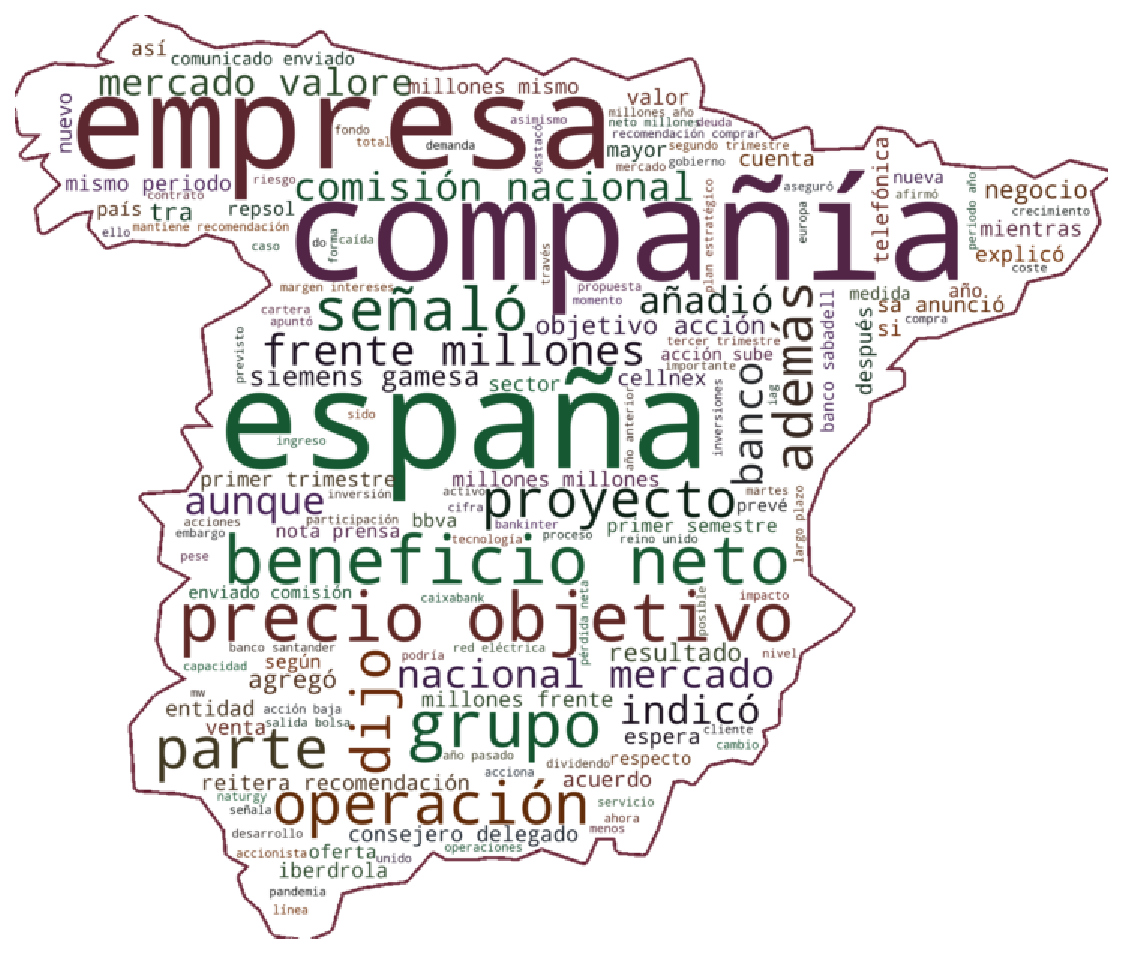
\includegraphics[scale=0.496]{/Users/jesusvillotamiranda/Library/CloudStorage/OneDrive-UniversidaddeLaRioja/CEMFI/__MSc__/__Second_year__/6th_Term/MasterThesis/__Output/EDA_WordCloud.pdf}
  \label{fig:WordCloud}
  \subcaption*{\textit{Note: This Word Cloud visualizes the most frequent words in our dataset of Spanish business news articles. Larger words correspond to higher frequencies. The color of the words is purely for visual differentiation and holds no additional meaning. The most prominent words include \qquote{empresa} (firm), \qquote{compa��a} (company), and \qquote{espa�a} (Spain), reinforcing that the dataset primarily comprises Spanish business news, with a prevalence of technical terms such as \qquote{beneficio neto} (net profit), \qquote{precio objetivo} (target price), \qquote{proyecto} (project), and \qquote{operaci�n} (operation).}}
\end{figure}
%----------------------------------------------------

The distribution of the number of articles published per day is illustrated in \cref{fig:hist_1}, showing that the most frequent publication rate is between 5 and 10 articles per day, though some days exhibit unusually high publication counts. \cref{fig:hist_2} shows the distribution of the number of words per article, with the majority of articles containing between 70 and 280 words. This indicates that the articles are relatively succinct, providing direct information. 
However, the long right tail points to instances of more comprehensive coverage.
%However, a small subset of articles exceeds 500 words, indicating more in-depth coverage.

%----------------------------------------------------
\inserthere{fig:histograms}
\begin{figure}[H]
  \caption{Histogram of \# News Articles per Day and \# Words per Article}
  \centering
  \begin{subfigure}[b]{0.46\textwidth}
    \centering
    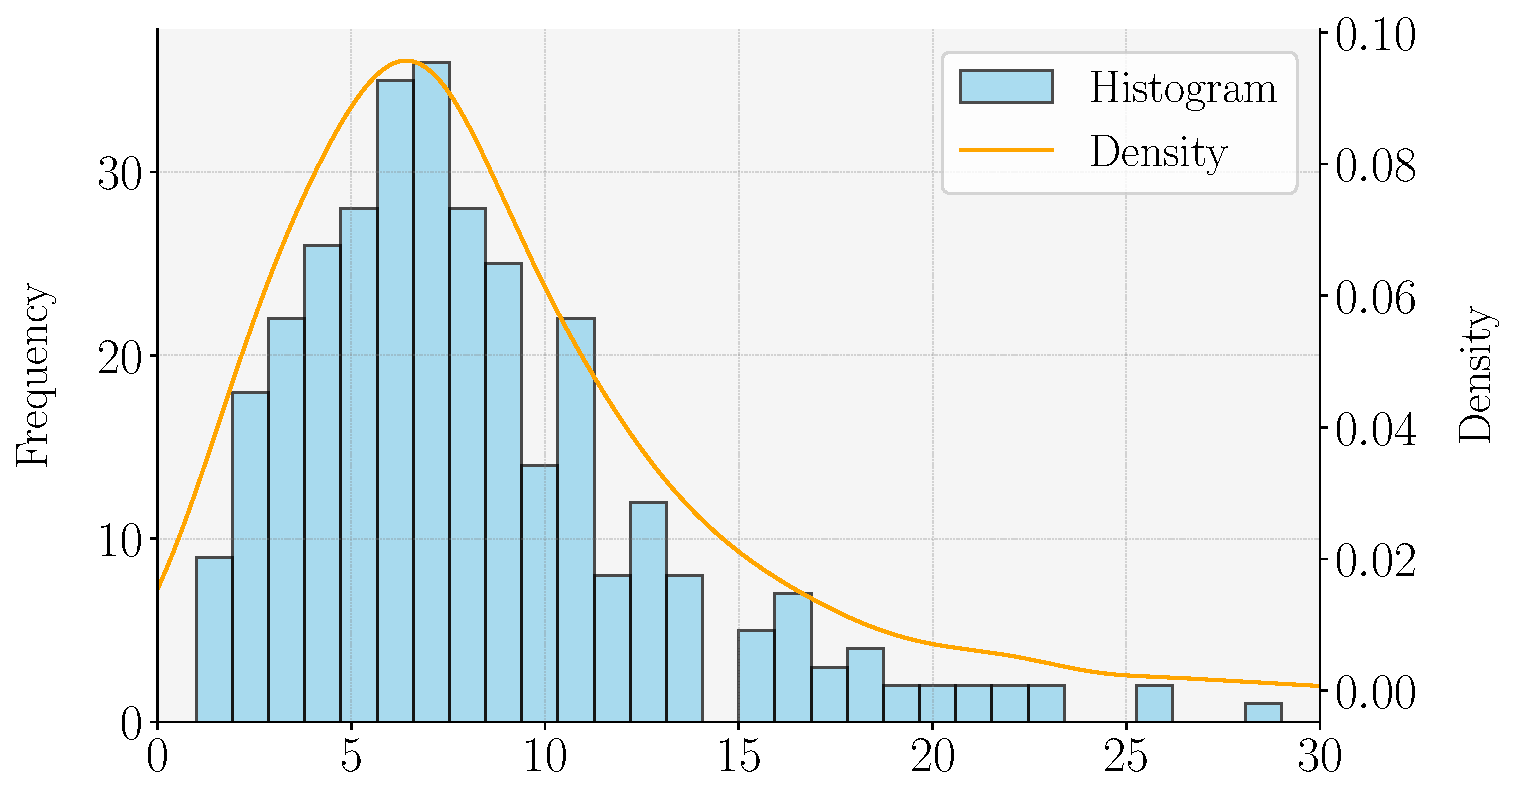
\includegraphics[width=\textwidth]{/Users/jesusvillotamiranda/Library/CloudStorage/OneDrive-UniversidaddeLaRioja/CEMFI/__MSc__/__Second_year__/6th_Term/MasterThesis/__Output/EDA_Histogram_of_Number_of_News_Articles_per_day.pdf}
    \caption{Number of News Articles per Day}
    \label{fig:hist_1}
  \end{subfigure}
  \hspace{0.05\textwidth} % Add horizontal space between the subfigures
  \begin{subfigure}[b]{0.46\textwidth}
    \centering
    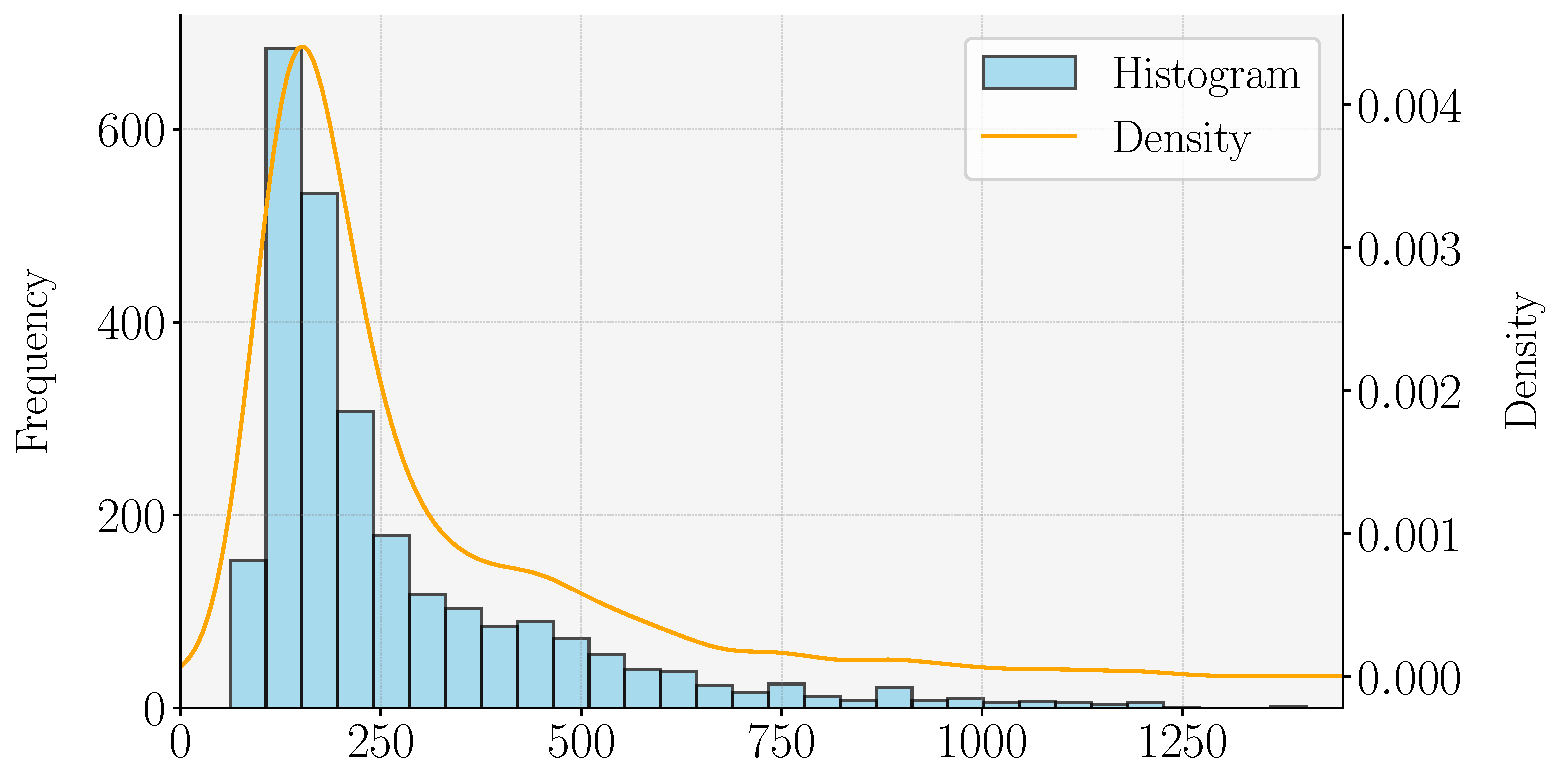
\includegraphics[width=\textwidth]{/Users/jesusvillotamiranda/Library/CloudStorage/OneDrive-UniversidaddeLaRioja/CEMFI/__MSc__/__Second_year__/6th_Term/MasterThesis/__Output/EDA_Number_of_Words_per_Article.pdf}
    \caption{Number of Words per Article}
    \label{fig:hist_2}
  \end{subfigure}
  \label{fig:histograms}
  \subcaption*{\textit{Note: Panel (a) displays the distribution of the number of news articles published per day, with most days having between 5 and 10 articles. Panel (b) shows the distribution of the number of words per article, where the majority are between 70 and 280 words, suggesting concise reporting. However, the long right tail indicates instances of more comprehensive coverage.}}

\end{figure}
%----------------------------------------------------

The time series of the number of articles published per day throughout the sample period is shown in \Cref{fig:ts_articles}. The series exhibits considerable variability, with frequent fluctuations from fewer than 5 articles per day to sudden spikes exceeding 20 articles. The 30-day moving average smooths the series, confirming the previous observation that, on average, between 5 and 10 articles are published daily.

%----------------------------------------------------
\inserthere{fig:ts_articles}
\begin{figure}[H]
  \centering
  \caption{Time Series of Number of Articles per Day and 30-Period Moving Average}
  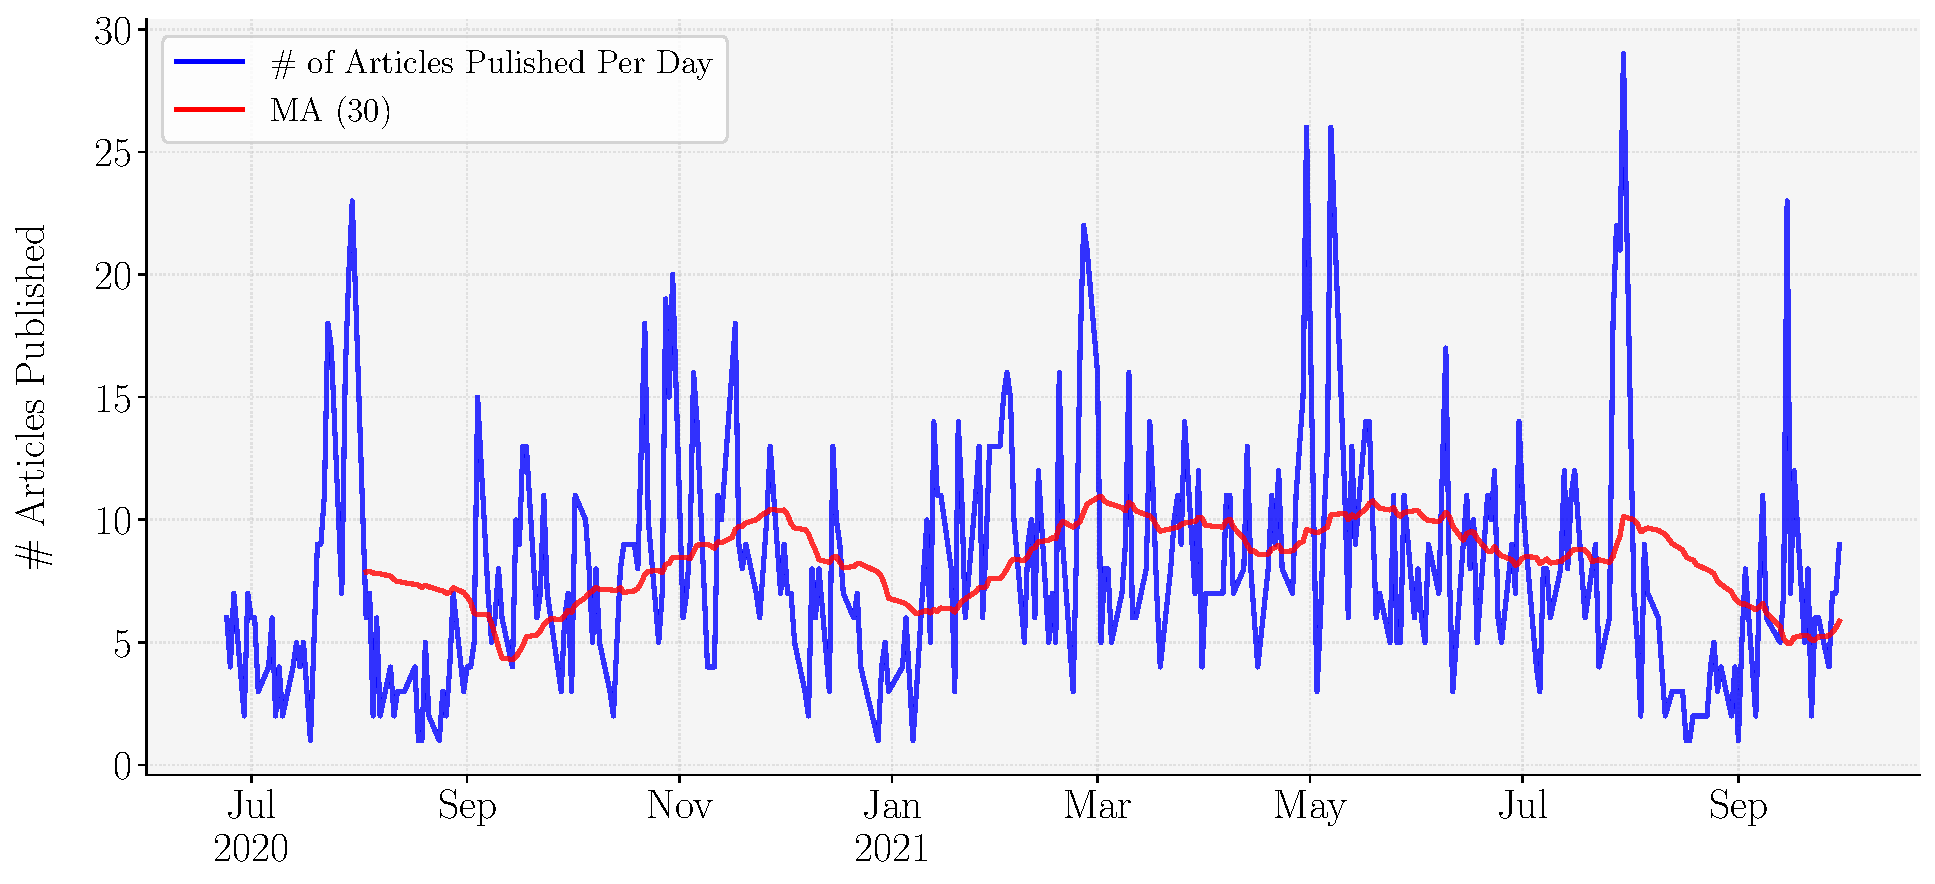
\includegraphics[scale=0.445]{/Users/jesusvillotamiranda/Library/CloudStorage/OneDrive-UniversidaddeLaRioja/CEMFI/__MSc__/__Second_year__/6th_Term/MasterThesis/__Output/EDA_Time_Series_of_Articles.pdf}
  \label{fig:ts_articles}
  \subcaption*{\textit{Note: The time series shows the daily number of news articles published, characterized by significant variability with occasional sharp spikes. The 30-day moving average smooths these fluctuations, revealing an average publication rate of 5 to 10 articles per day.}}
\end{figure}
%----------------------------------------------------

%%%%%%%%%%%%%%%%% METHODOLOGY %%%%%%%%%%%%%%%%%%%%%%
\section{Mathematical Treatment of News Articles}

 \hspace{0.5cm} 
 Our dataset consists of $N=2,613$ Spanish business news articles 
 sourced from DowJones and spanning the period from 2020/06/24 to 2021/09/30. 
 We denote as $\mathcal D$ the set of all articles in our sample.
 % from DowJones for the period 2020-6-24 to 2021-09-30. 
 These articles have been specifically filtered to reference firms listed on the IBEX-35.
% These articles have been specifically filtered to be explicitly referred to firms that are listed in the IBEX-35.
 Let $\F_{\t{IBEX35}}$ denote the universe of such firms. 
 Each article $i \in \mathcal{D}$ is a textual document detailing an event that directly pertains to a subset of firms $\mathcal{F}^i \subseteq \F_{\t{IBEX35}}$.
% Each article $i\in \D$ is a textual document narrating an event that directly involves a set of firms %$\F^i \subseteq \F_{\t{IBEX35}}$.
%
The publication date and time of each article are represented as $\mathcal{Y}_0^i = \langle d_0^i, t_0^i \rangle$, where $d_0^i$ captures the date 
(YYYY-MM-DD) 
and $t_0^i$ captures the time
 (HH:MM) 
 of publication. 
%This datetime representation emphasizes 
Therefore we observe
the moment at which $\mathcal{F}^i$ receives the \qquote{treatment} of public news dissemination. 
%The information conveyed by an article can then be represented in a tuple 
%$
%\langle i, \F^i , \mathcal Y_0^i \rangle 
%$

%The article is published at some datetime represented by a tuple $\mathcal Y_0^i :=\angl{d_0^i, t_0^i}$, where $d_0^i$ represents the date component (YYYY-MM-DD) and $t_0^i$ represents the time component (HH:MM:SS.SSS). We use a 0-subscript to emphasize that $\mathcal Y_0^i$ is the day and time in which $\mathcal F^i$  receives  ``treatment'' (publication of a news article directly involving $\mathcal F^i$).
%%``treatment date'' or day in which a news article is published regarding firm $j$ (firm $j$ receives treatment) 
%

%\mx 
\subsubsection*{Data Splitting}
For robust model development and evaluation, the dataset is partitioned into three sequential subsets: training, validation, and test:
$
\D := \D^{tr} \cup \D^{val} \cup \D^{test}.
$
Define $N_{split}:=|\D^{split}|$ for $split\in\3{tr,val,test}$, where $\abs{\cd}$ denotes the cardinality of a set. 
%Then, it follows that
%%with $N_{tr}:=\abs{\D^{tr}}, N_{val}:=\abs{\D^{val}}$, N_{test}:=\abs{\D^{test}}$ 
%$\abs{\D}= N_{tr} + N_{val} + N_{test} = N$. 
%----------------------------------------------------
%The training and validation samples represent 80\% of the total sample $(\frac{N_{tr}+N_{val}}{N} = 0.8)$ and are used to design the optimal trading strategy, while the test sample represents the remaining 20\% $(\frac{N_{test}}{N} = 0.2)$ and is used to evaluate the \textit{out-of-sample} performance of the strategy. 
%--------- CHAT GPT OPTION ---------%
The training and validation sets collectively comprise 80\% of the total dataset $(\frac{N_{\text{tr}} + N_{\text{val}}}{N} = 0.8)$ and are instrumental in constructing and fine-tuning the trading strategy. The remaining 20\% $(\frac{N_{\text{test}}}{N} = 0.2)$ is reserved for out-of-sample testing to assess the performance and generalizability of the strategy under unseen conditions.
%----------------------------------------------------

%%%%%%%%%%%%%%%%%%%%%%%%%%%%%%%%%%%%%%%%%%%%%%%%%%%%%
%%%%%%%%%%%%%%%%%%%%%%%%%%%%%%%%%%%%%%%%%%%%%%%%%%%%%
\subsubsection*{Effective treatment day}
\hspace{0.5cm} We are interested in examining the impact of each news article $i\in\D$ on the stock price of the firms that are affected directly (i.e.: all $j\in\F^i$). Since the publication datetime is not necessarily a trading datetime, we cannot directly gauge such an effect by looking at $\mathcal Y_0^i$. 
For this reason, we need to work through some definitions. 
%
%$(\tilde{d}_0^i)$ as the date at which news article $i$ events can be incorporated into the stock prices of $\F^i$. 
%
Let $\T$ denote the set of all datetimes in the sample timeline and let $\widetilde{\T}\subset \T$ be the subset of Spanish trading datetimes associated to our sample.
\begin{align*}
\widetilde{\T} := 
\3{\angl{d,t} \mid d \in \tilde{\mathfrak d} ~\wedge~ t\in \tilde{\mathfrak t}}
,
\end{align*}
where 
$
\tilde{\mathfrak{d}}:=\{\tilde{\mathfrak{d}}_{[1]},\tilde{\mathfrak{d}}_{[2]}, \ldots \tilde{\mathfrak{d}}_{[n]}\}
$
is the ordered set of week and non-festive days according to the Spanish calendar in our data timeline,
%, and $\tilde{\mathfrak t}$ are the trading hours 
and 
$\tilde{\mathfrak t}:=
\{t \mid \t{09:30} \leq t \leq  \t{17:30}\}
%\{t \mid t\in\t[\t{09:30}, \t{17:30}]\}
$
 are the Spanish stock market trading hours. 
Note that we use tildes to emphasize that we are considering trading dates or times. 

%We can now define a set of functions that will become useful as we work with trading days.
%We now introduce some functions that will prove useful now and later on for easily handling trading days. 

%%----------------------------------------------------
%
\textbf{Index Function}. 
Given a finite ordered set $\mathcal{Z}=\left\{z_1, z_2, \ldots, z_n\right\}$, the index function 
$\mathbb{I}_{\mathcal{Z}}: \mathcal{Z} \rightarrow\{1,2, \ldots,|\mathcal{Z}|\}$
%$\mathbb{I}_{\mathcal{Z}}(z)$
 maps an element $z\in\Z$ to its position in the ordered set $\mathcal{Z}$. Formally:
$$
\mathbb{I}_{\mathcal{Z}}(z_{\ell})=\ell 
%\quad \text { if and only if } \quad z=z_{\ell} 
\quad \text { for } \quad \ell \in\{1,2, \ldots,|\mathcal{Z}|\}
$$
%where $z_{\ell}$ denotes the ${\ell}$-th element of the ordered set $\mathcal{Z}$.

\textbf{Inverse Index Function}. 
The inverse index function 
$\mathbb{I}_{\mathcal{Z}}^{-1}:\{1,2, \ldots,|\mathcal{Z}|\} \rightarrow \mathcal{Z}$
%$\mathbb{I}_{\mathcal{Z}}^{-1}({\ell})$
 retrieves the element $z \in \mathcal{Z}$ corresponding to a given index ${\ell}$.
Formally:
$$
\mathbb{I}_{\mathcal{Z}}^{-1}({\ell})=z_{\ell} \quad \text { for } \quad {\ell} \in\{1,2, \ldots,|\mathcal{Z}|\}
$$

%Properties
%1. Index Function: $\mathbb{I}_{\mathcal{Z}}: \mathcal{Z} \rightarrow\{1,2, \ldots,|\mathcal{Z}|\}$
%2. Inverse Index Function: $\mathbb{I}_{\mathcal{Z}}^{-1}:\{1,2, \ldots,|\mathcal{Z}|\} \rightarrow \mathcal{Z}$

%%%%%%%%%%%%%%%%%%%%%%%%%%%%%%%%%%%%%%%%%%%%%%%%%%%%%%
%%%%%%%%%%%%%%%% Updated: 17th July %%%%%%%%%%%%%%%%%%
%%%%%%%%%%%%%%%%%%%%%%%%%%%%%%%%%%%%%%%%%%%%%%%%%%%%%%
\begin{table}[H]
\centering
\renewcommand{\arraystretch}{1.4}
{\small
\begin{tabular}{L{9.9cm}|L{6.5cm}}
\hline
\multicolumn{1}{c|}{\textit{Function}}  & \multicolumn{1}{c}{\textit{Definition}}\\ \hline
%\toprule 
%\hline
%----------------------------------------------------
\textbf{Index Function} 

$~\bullet~$ Maps an element $z\in\Z$ to its position in $\Z$

$~\bullet~$ $\mathbb{I}_{\Z}: \Z \to 
\3{1,2,...,\abs{\Z}}
%\3{n\in \mathbb{N} \mid 1\leq n \leq \abs{\Z}}
$ 
&
$
~~\mathbb{I}_{\Z}(z) 
=
b, \qquad z = \Z_{[b]}
%\begin{cases} 
%	k & \text{if~~~} d = \tilde{\mathfrak{d}}_{[k]} \in \tilde{\mathfrak{d}} 
%	\\ 
%	\emptyset & \text{if~~~} d \medskip\notin \tilde{\mathfrak{d}} 
%\end{cases}
$
\\ 
\hline 
%----------------------------------------------------
\textbf{Inverse Index Function}

$~\bullet~$ Retrieves the element $z\in\Z$ corresponding to an index

$~\bullet~$ $\mathbb{I}^{-1}_{\Z}: \{1, 2, \ldots, 
\abs{Z}
%|\tilde{\mathfrak{d}}|
\} \to \Z$ 
&
~~$\mathbb{I}^{-1}_{\Z}(b) 
= 
\Z_{[b]}  
,\quad
b \in \{1, 2, \ldots, \abs{Z}\} 
%\begin{cases} 
%	\tilde{\mathfrak{d}}_{[k]} & \text{if~~~} k \in \{1, 2, \ldots, 
%	Z
%	\} 
%	\\ 
%	\emptyset & \text{if~~~} k \notin \{1, 2, \ldots, 
%	Z
%	\} 
%\end{cases}
$
\\ 
\hline
%----------------------------------------------------
\textbf{Closest Trading Day Function} 


$~\bullet~$ Returns the next closest trading day to $d\in\mathfrak{d}$ within $\tilde{\mathfrak{d}}$

$~\bullet~$ $\Lambda: \mathfrak{d} \to \tilde{\mathfrak{d}}$
&
~~
$\Lambda(d) 
:= 
\min \3{ \tilde{d} \in \tilde{\mathfrak{d}} \mid \tilde{d} \geq d }$
\\
\hline
\end{tabular}
}
\end{table}
%%%%%%%%%%%%%%%%%%%%%%%%%%%%%%%%%%%%%%%%%%%%%%%%%%%%%




%%%%%%%%%%%%%%%%%%%%%%%%%%%%%%%%%%%%%%%%%%%%%%%%%%%%%%%
%%%%%%% This was the table used before 17th July %%%%%% 
%%%%%%%%%%%%%%%%%%%%%%%%%%%%%%%%%%%%%%%%%%%%%%%%%%%%%%%
%
%\begin{table}[H]
%\centering
%\renewcommand{\arraystretch}{1.4}
%{\small
%\begin{tabular}{L{9.9cm}|L{6.5cm}}
%\hline
%\multicolumn{1}{c|}{\textit{Function}}  & \multicolumn{1}{c}{\textit{Definition}}\\ \hline
%%\toprule 
%%\hline
%%----------------------------------------------------
%\textbf{Index Function} 
%
%$~\bullet~$ Maps a trading day $d \in \tilde{\mathfrak{d}}$ to its position in $\tilde{\mathfrak{d}}$
%
%$~\bullet~$ $\mathbb{I}_{\tilde{\mathfrak{d}}}: \tilde{\mathfrak{d}} \to \{1, 2, \ldots, Z
%\}$ 
%&
%$
%~~\mathbb{I}_{\tilde{\mathfrak{d}}}(d) 
%=
%k, \qquad d = \tilde{\mathfrak{d}}_{[k]} \in \tilde{\mathfrak{d}} 
%%\begin{cases} 
%%	k & \text{if~~~} d = \tilde{\mathfrak{d}}_{[k]} \in \tilde{\mathfrak{d}} 
%%	\\ 
%%	\emptyset & \text{if~~~} d \medskip\notin \tilde{\mathfrak{d}} 
%%\end{cases}
%$
%\\ 
%\hline 
%%----------------------------------------------------
%\textbf{Inverse Index Function}
%
%$~\bullet~$ Retrieves the trading day corresponding to an index
%
%$~\bullet~$ $\mathbb{D}_{\tilde{\mathfrak{d}}}: \{1, 2, \ldots, 
%Z
%%|\tilde{\mathfrak{d}}|
%\} \to \tilde{\mathfrak{d}}$ 
%&
%~~$\mathbb{D}_{\tilde{\mathfrak{d}}}(k) 
%= 
%\tilde{\mathfrak{d}}_{[k]}  
%,\quad
%k \in \{1, 2, \ldots, Z\} 
%%\begin{cases} 
%%	\tilde{\mathfrak{d}}_{[k]} & \text{if~~~} k \in \{1, 2, \ldots, 
%%	Z
%%	\} 
%%	\\ 
%%	\emptyset & \text{if~~~} k \notin \{1, 2, \ldots, 
%%	Z
%%	\} 
%%\end{cases}
%$
%\\ 
%\hline
%%----------------------------------------------------
%\textbf{Closest Trading Day Function} 
%
%
%$~\bullet~$ Returns the next closest trading day to $d\in\mathfrak{d}$ within $\tilde{\mathfrak{d}}$
%
%$~\bullet~$ $\Lambda: \mathfrak{d} \to \tilde{\mathfrak{d}}$
%&
%~~$\Lambda(d) 
%:= 
%\min \left\{ \tilde{d} \in \tilde{\mathfrak{d}} \mid \tilde{d} \geq d \right\}$
%\\
%\hline
%\end{tabular}
%}
%\end{table}
%%%%%%%%%%%%%%%%%%%%%%%%%%%%%%%%%%%%%%%%%%%%%%%%%%%%%%

%%----------------------------------------------------

\bx 
Throughout our analysis, we will work with daily stock market closing data for each trading day. However, we will exploit the time component of $\mathcal Y_0^i$ to assign an \qquote{effective treatment date} to each article. Namely, define $\tilde d_0^i$ as the day at which article $i$'s information can be incorporated into the stock market; then, $\tilde d_0^i$ is the publication date if the article was published on a trading day before the stock market was closed, and is equal to the next closest trading day otherwise. 
To compute the next closest trading day to $d\in\mathfrak d$ within $\tilde{\mathfrak d}$, we need to work with a function $\Lambda:\mathfrak d \to \tilde{\mathfrak d}$ such that  
$\Lambda(d) 
:= 
\min \{ \tilde{d} \in \tilde{\mathfrak{d}} \mid \tilde{d} \geq d \}$. 
Thus, now we can define:
\begin{align*}
\tilde{d}_0^i :=
\mycases{llll}{
d_0^i & \IF & d_0^i \in \tilde{\mathfrak d} ~\wedge~t_0^i < \t{17:30}
\\
\Lambda(d_0^i)
& \IF & d_0^i \not \in \tilde{\mathfrak d} ~\vee~t_0^i \geq  \t{17:30}
}
.
\end{align*}


\section{Clustering News Articles}

\hspace{0.5cm}In this section we present our clustering methodology based on news-implied firm-specific shock classifications and we compare it against a benchmark based on clustering the vector embedding representations of the articles. For ease of exposition, we will first present the benchmark model.

%----------------------------------------------------
 \hspace{0.5cm} Our dataset $\mathcal D$ consists of $N=2,613$ Spanish business news articles 
 sourced from DowJones and spanning the period from June 24, 2020, to September 30, 2021. 
 % from DowJones for the period 2020-6-24 to 2021-09-30. 
 These articles have been specifically filtered to reference firms listed on the IBEX-35.
% These articles have been specifically filtered to be explicitly referred to firms that are listed in the IBEX-35.
 Let $\F_{\t{IBEX35}}$ denote the universe of such firms. 
 Each article $i \in \mathcal{D}$ is a textual document detailing an event that directly pertains to a subset of firms $\mathcal{F}^i \subseteq \F_{\t{IBEX35}}$.
% Each article $i\in \D$ is a textual document narrating an event that directly involves a set of firms %$\F^i \subseteq \F_{\t{IBEX35}}$.
%
The publication date and time of each article are represented as $\mathcal{Y}_0^i := \langle d_0^i, t_0^i \rangle$, where $d_0^i$ captures the date (YYYY-MM-DD) and $t_0^i$ captures the time (HH:MM
.SSS) of publication. This datetime representation emphasizes the moment at which $\mathcal{F}^i$ receives the \qquote{treatment} of public news dissemination. 
%The information conveyed by an article can then be represented in a tuple 
%$
%\langle i, \F^i , \mathcal Y_0^i \rangle 
%$

%The article is published at some datetime represented by a tuple $\mathcal Y_0^i :=\angl{d_0^i, t_0^i}$, where $d_0^i$ represents the date component (YYYY-MM-DD) and $t_0^i$ represents the time component (HH:MM:SS.SSS). We use a 0-subscript to emphasize that $\mathcal Y_0^i$ is the day and time in which $\mathcal F^i$  receives  ``treatment'' (publication of a news article directly involving $\mathcal F^i$).
%%``treatment date'' or day in which a news article is published regarding firm $j$ (firm $j$ receives treatment) 
%

\mx 
For robust model development and evaluation, the dataset is partitioned into three sequential subsets: training, validation, and test
$
\D := [\D^{tr}, \D^{val}, \D^{test}].
$
Define $N_{split}:=|\D^{split}|$ for $split\in\3{tr,val,test}$, where $\abs{\cd}$ denotes the cardinality of a set. 
Then, it follows that
%with $N_{tr}:=\abs{\D^{tr}}, N_{val}:=\abs{\D^{val}}$, N_{test}:=\abs{\D^{test}}$ 
$\abs{\D}= N_{tr} + N_{val} + N_{test} = N$. 
%----------------------------------------------------
%The training and validation samples represent 80\% of the total sample $(\frac{N_{tr}+N_{val}}{N} = 0.8)$ and are used to design the optimal trading strategy, while the test sample represents the remaining 20\% $(\frac{N_{test}}{N} = 0.2)$ and is used to evaluate the \textit{out-of-sample} performance of the strategy. 
%--------- CHAT GPT OPTION ---------%
The training and validation sets collectively comprise 80\% of the total dataset $(\frac{N_{\text{tr}} + N_{\text{val}}}{N} = 0.8)$ and are instrumental in constructing and fine-tuning the trading strategy. The remaining 20\% $(\frac{N_{\text{test}}}{N} = 0.2)$ is reserved for out-of-sample testing to assess the performance and generalizability of the strategy under unseen conditions.
%----------------------------------------------------

%%%%%%%%%%%%%%%%%%%%%%%%%%%%%%%%%%%%%%%%%%%%%%%%%%%%%
%%%%%%%%%%%%%%%%%%%%%%%%%%%%%%%%%%%%%%%%%%%%%%%%%%%%%
\subsection{Publication datetime \& Effective treatment day}
\hspace{0.5cm} We are interested in examining the impact of each news article $i\in\D$ on the stock price of the firms that are affected directly (i.e.: all $j\in\F^i$). Since the publication datetime is not necessarily a trading datetime, we cannot directly gauge such an effect by looking at $\mathcal Y_0^i$. 
For this reason, we need to work through some definitions. 
%
%$(\tilde{d}_0^i)$ as the date at which news article $i$ events can be incorporated into the stock prices of $\F^i$. 
%
Let $\T$ denote the set of all datetimes in the sample timeline and let $\widetilde{\T}\subset \T$ be the subset of Spanish trading datetimes associated to our sample.
\begin{align*}
\widetilde{\T} := 
\3{\angl{d,t} \mid d \in \tilde{\mathfrak d} ~\wedge~ t\in \tilde{\mathfrak t}}
,
\end{align*}
where 
$
\tilde{\mathfrak{d}}:=\{\tilde{\mathfrak{d}}_{[1]},\tilde{\mathfrak{d}}_{[2]}, \ldots \tilde{\mathfrak{d}}_{[n]}\}
$
is the ordered set of week and non-festive days according to the Spanish calendar in our data timeline,
%, and $\tilde{\mathfrak t}$ are the trading hours 
and 
$\tilde{\mathfrak t}:=
\{t \mid \t{09:30} \leq t \leq  \t{17:30}\}
%\{t \mid t\in\t[\t{09:30}, \t{17:30}]\}
$
 are the Spanish stock market trading hours. 
Note that we use tildes to emphasize that we are considering trading dates or times. 

%We can now define a set of functions that will become useful as we work with trading days.
%We now introduce some functions that will prove useful now and later on for easily handling trading days. 

%%----------------------------------------------------
%
\textbf{Index Function}. 
Given a finite ordered set $\mathcal{Z}=\left\{z_1, z_2, \ldots, z_n\right\}$, the index function 
$\mathbb{I}_{\mathcal{Z}}: \mathcal{Z} \rightarrow\{1,2, \ldots,|\mathcal{Z}|\}$
%$\mathbb{I}_{\mathcal{Z}}(z)$
 maps an element $z\in\Z$ to its position in the ordered set $\mathcal{Z}$. Formally:
$$
\mathbb{I}_{\mathcal{Z}}(z_{\ell})=\ell 
%\quad \text { if and only if } \quad z=z_{\ell} 
\quad \text { for } \quad \ell \in\{1,2, \ldots,|\mathcal{Z}|\}
$$
%where $z_{\ell}$ denotes the ${\ell}$-th element of the ordered set $\mathcal{Z}$.

\textbf{Inverse Index Function}. 
The inverse index function 
$\mathbb{I}_{\mathcal{Z}}^{-1}:\{1,2, \ldots,|\mathcal{Z}|\} \rightarrow \mathcal{Z}$
%$\mathbb{I}_{\mathcal{Z}}^{-1}({\ell})$
 retrieves the element $z \in \mathcal{Z}$ corresponding to a given index ${\ell}$.
Formally:
$$
\mathbb{I}_{\mathcal{Z}}^{-1}({\ell})=z_{\ell} \quad \text { for } \quad {\ell} \in\{1,2, \ldots,|\mathcal{Z}|\}
$$

%Properties
%1. Index Function: $\mathbb{I}_{\mathcal{Z}}: \mathcal{Z} \rightarrow\{1,2, \ldots,|\mathcal{Z}|\}$
%2. Inverse Index Function: $\mathbb{I}_{\mathcal{Z}}^{-1}:\{1,2, \ldots,|\mathcal{Z}|\} \rightarrow \mathcal{Z}$

%%%%%%%%%%%%%%%%%%%%%%%%%%%%%%%%%%%%%%%%%%%%%%%%%%%%%%
%%%%%%%%%%%%%%%% Updated: 17th July %%%%%%%%%%%%%%%%%%
%%%%%%%%%%%%%%%%%%%%%%%%%%%%%%%%%%%%%%%%%%%%%%%%%%%%%%
\begin{table}[H]
\centering
\renewcommand{\arraystretch}{1.4}
{\small
\begin{tabular}{L{9.9cm}|L{6.5cm}}
\hline
\multicolumn{1}{c|}{\textit{Function}}  & \multicolumn{1}{c}{\textit{Definition}}\\ \hline
%\toprule 
%\hline
%----------------------------------------------------
\textbf{Index Function} 

$~\bullet~$ Maps an element $z\in\Z$ to its position in $\Z$

$~\bullet~$ $\mathbb{I}_{\Z}: \Z \to 
\3{1,2,...,\abs{\Z}}
%\3{n\in \mathbb{N} \mid 1\leq n \leq \abs{\Z}}
$ 
&
$
~~\mathbb{I}_{\Z}(z) 
=
b, \qquad z = \Z_{[b]}
%\begin{cases} 
%	k & \text{if~~~} d = \tilde{\mathfrak{d}}_{[k]} \in \tilde{\mathfrak{d}} 
%	\\ 
%	\emptyset & \text{if~~~} d \medskip\notin \tilde{\mathfrak{d}} 
%\end{cases}
$
\\ 
\hline 
%----------------------------------------------------
\textbf{Inverse Index Function}

$~\bullet~$ Retrieves the element $z\in\Z$ corresponding to an index

$~\bullet~$ $\mathbb{I}^{-1}_{\Z}: \{1, 2, \ldots, 
\abs{Z}
%|\tilde{\mathfrak{d}}|
\} \to \Z$ 
&
~~$\mathbb{I}^{-1}_{\Z}(b) 
= 
\Z_{[b]}  
,\quad
b \in \{1, 2, \ldots, \abs{Z}\} 
%\begin{cases} 
%	\tilde{\mathfrak{d}}_{[k]} & \text{if~~~} k \in \{1, 2, \ldots, 
%	Z
%	\} 
%	\\ 
%	\emptyset & \text{if~~~} k \notin \{1, 2, \ldots, 
%	Z
%	\} 
%\end{cases}
$
\\ 
\hline
%----------------------------------------------------
\textbf{Closest Trading Day Function} 


$~\bullet~$ Returns the next closest trading day to $d\in\mathfrak{d}$ within $\tilde{\mathfrak{d}}$

$~\bullet~$ $\Lambda: \mathfrak{d} \to \tilde{\mathfrak{d}}$
&
~~
$\Lambda(d) 
:= 
\min \3{ \tilde{d} \in \tilde{\mathfrak{d}} \mid \tilde{d} \geq d }$
\\
\hline
\end{tabular}
}
\end{table}
%%%%%%%%%%%%%%%%%%%%%%%%%%%%%%%%%%%%%%%%%%%%%%%%%%%%%




%%%%%%%%%%%%%%%%%%%%%%%%%%%%%%%%%%%%%%%%%%%%%%%%%%%%%%%
%%%%%%% This was the table used before 17th July %%%%%% 
%%%%%%%%%%%%%%%%%%%%%%%%%%%%%%%%%%%%%%%%%%%%%%%%%%%%%%%
%
%\begin{table}[H]
%\centering
%\renewcommand{\arraystretch}{1.4}
%{\small
%\begin{tabular}{L{9.9cm}|L{6.5cm}}
%\hline
%\multicolumn{1}{c|}{\textit{Function}}  & \multicolumn{1}{c}{\textit{Definition}}\\ \hline
%%\toprule 
%%\hline
%%----------------------------------------------------
%\textbf{Index Function} 
%
%$~\bullet~$ Maps a trading day $d \in \tilde{\mathfrak{d}}$ to its position in $\tilde{\mathfrak{d}}$
%
%$~\bullet~$ $\mathbb{I}_{\tilde{\mathfrak{d}}}: \tilde{\mathfrak{d}} \to \{1, 2, \ldots, Z
%\}$ 
%&
%$
%~~\mathbb{I}_{\tilde{\mathfrak{d}}}(d) 
%=
%k, \qquad d = \tilde{\mathfrak{d}}_{[k]} \in \tilde{\mathfrak{d}} 
%%\begin{cases} 
%%	k & \text{if~~~} d = \tilde{\mathfrak{d}}_{[k]} \in \tilde{\mathfrak{d}} 
%%	\\ 
%%	\emptyset & \text{if~~~} d \medskip\notin \tilde{\mathfrak{d}} 
%%\end{cases}
%$
%\\ 
%\hline 
%%----------------------------------------------------
%\textbf{Inverse Index Function}
%
%$~\bullet~$ Retrieves the trading day corresponding to an index
%
%$~\bullet~$ $\mathbb{D}_{\tilde{\mathfrak{d}}}: \{1, 2, \ldots, 
%Z
%%|\tilde{\mathfrak{d}}|
%\} \to \tilde{\mathfrak{d}}$ 
%&
%~~$\mathbb{D}_{\tilde{\mathfrak{d}}}(k) 
%= 
%\tilde{\mathfrak{d}}_{[k]}  
%,\quad
%k \in \{1, 2, \ldots, Z\} 
%%\begin{cases} 
%%	\tilde{\mathfrak{d}}_{[k]} & \text{if~~~} k \in \{1, 2, \ldots, 
%%	Z
%%	\} 
%%	\\ 
%%	\emptyset & \text{if~~~} k \notin \{1, 2, \ldots, 
%%	Z
%%	\} 
%%\end{cases}
%$
%\\ 
%\hline
%%----------------------------------------------------
%\textbf{Closest Trading Day Function} 
%
%
%$~\bullet~$ Returns the next closest trading day to $d\in\mathfrak{d}$ within $\tilde{\mathfrak{d}}$
%
%$~\bullet~$ $\Lambda: \mathfrak{d} \to \tilde{\mathfrak{d}}$
%&
%~~$\Lambda(d) 
%:= 
%\min \left\{ \tilde{d} \in \tilde{\mathfrak{d}} \mid \tilde{d} \geq d \right\}$
%\\
%\hline
%\end{tabular}
%}
%\end{table}
%%%%%%%%%%%%%%%%%%%%%%%%%%%%%%%%%%%%%%%%%%%%%%%%%%%%%%

%%----------------------------------------------------

\bx 
Throughout our analysis, we will work with daily stock market closing data for each trading day. However, we will exploit the time component of $\mathcal Y_0^i$ to assign an \qquote{effective treatment date} to each article. Namely, define $\tilde d_0^i$ as the day at which article $i$'s information can be incorporated into the stock market; then, $\tilde d_0^i$ is the publication date if the article was published on a trading day before the stock market was closed, and is equal to the next closest trading day otherwise. 
To compute the next closest trading day to $d\in\mathfrak d$ within $\tilde{\mathfrak d}$, we need to work with a function $\Lambda:\mathfrak d \to \tilde{\mathfrak d}$ such that  
$\Lambda(d) 
:= 
\min \{ \tilde{d} \in \tilde{\mathfrak{d}} \mid \tilde{d} \geq d \}$. 
Thus, now we can define:
\begin{align*}
\tilde{d}_0^i :=
\mycases{llll}{
d_0^i & \IF & d_0^i \in \tilde{\mathfrak d} ~\wedge~t_0^i < \t{17:30}
\\
\Lambda(d_0^i)
& \IF & d_0^i \not \in \tilde{\mathfrak d} ~\vee~t_0^i \geq  \t{17:30}
}
.
\end{align*}



%%%%%%%%%%%%%%%%%%%%%%%%%%%%%%%%%%%%%%%%%%%%%%%%%%%%%
%%%%%%%%%%%%%%%%%%%%%%%%%%%%%%%%%%%%%%%%%%%%%%%%%%%%%
\subsection{Transforming text into numerical data}


\hspace{0.5cm} Any piece of text can be represented as a high-dimensional vector embedding by using a transformer. Transformers are a type of deep learning architecture introduced by \cite{vaswani2017attention} which have revolutionized natural language processing (\texttt{NLP}). The core idea behind them is the self-attention mechanism, which allows the model to weigh the importance of different words in a sentence when generating a representation for each word. This mechanism enables transformers to capture long-range dependencies and contextual relationships within the text more effectively than previous models like recurrent neural networks (\texttt{RNN}s).

\mx
A transformer model consists of an encoder and a decoder, both of which are composed of multiple layers of self-attention and feedforward neural networks. In our context, we primarily use the encoder to convert a piece of text into a fixed-size vector, known as an embedding. 
Since our articles are written in Spanish, we employ a \texttt{Multilingual Sentence Transformer}, which has been trained on text from multiple languages. 
%This ensures that the model can effectively understand and represent the meaning of Spanish text in a similar way it does for other languages. The multilingual model leverages cross-lingual learning, enabling it to generalize knowledge from one language to another.

\mx 
For every news article $i\in\D$, we obtain a representative vector embedding $\mathbf{e}^i \in \mathbb{R}^{512}$ that provides a numerical representation of 
%the semantic meaning of the events narrated therein. 
%These embeddings are created by passing the text through a pre-trained transformer model, which has learned to encode linguistic information into high-dimensional vectors during its training on large corpora of text. 
%
%The embeddings capture various aspects of the text, such as syntactic structure, semantic content, and contextual nuances.
%
%\mx 
%The embeddings generated by transformer models are high-dimensional vectors that captures 
%different aspect of the text's meaning. 
various aspects of the text, such as syntactic structure, semantic content, and contextual nuances.
%
%However, these dimensions are not always directly interpretable in isolation. Instead, they should be viewed as capturing complex patterns and relationships within the text data.
%
%
%To provide an example, consider a 512-dimensional embedding vector $\mathbf{e}^i$ for a news article. 
While it is challenging to assign a specific human-readable meaning to each of the 512 components, we can interpret the vector as a whole in various ways:


\begin{itemize}
  \item \textit{Semantic Similarity}: Similar articles will have similar embeddings. For instance, if one article discusses a company's quarterly earnings and another article discusses the same company's annual earnings, their embeddings will be close in the 512-dimensional space.
  \item \textit{Topic Clustering}: Articles on similar topics will cluster together. For example, articles about financial markets might cluster in one region of the embedding space, while articles about mergers and acquisitions cluster in another.
  \item \textit{Sentiment Analysis}: Different regions of the embedding space can implicitly represent different sentiments. Articles with positive news might cluster in one area, while those with negative news cluster in another.

\end{itemize}



%----------------------------------------------------
%Any piece of text can be represented as a high-dimensional vector embedding by using a transformer model. For every news article in our database, we obtain a representative embedding vector $\mbf e^i\in \R^{512}$ that provides a numerical representation of the semantic meaning of the events narrated therein. Since our articles are written in Spanish, we employ a \texttt{Multilingual Sentence Transformer}, which has been trained on text from multiple languages. 


%\Vhrulefill
%Hence, we can summarize the content of an article $i$ in a tuple
%$$
%\mathcal{A}^i := 
%\flexangl{
%%\mathcal Y_0^i, 
%%~
%\mbf e^i
%,~
%\F^i
%,~
%\tilde{d}_0^i
%}
%.
%$$

\subsection{Clustering embeddings with KMeans}


\hspace{0.5cm} With the numerical representation of each article in the form of embeddings $\{\mbf e^i\}_{i\in\D}$, we now seek to identify groups of similar articles. 
%This is achieved by applying clustering techniques.  
%
Namely, we use the \texttt{KMeans} algorithm, a popular clustering method that assigns a set of vectors into $k$ clusters
$\mathcal G:=\{1,2,...,k\}$ to minimize the within-cluster sum of squares (WCSS). 
The implementation of this clustering algorithm is methodically presented in the Appendix (\cref{alg:KMeans}). 
Each cluster $g\in\mathcal G$ defines a centroid $\mbf c_g$, which is the average vector of all the members of a cluster.
%
%The optimal cluster aggrupation of news articles is determined in the training sample by fitting the \texttt{KMeans} algorithm to the embedding vectors. 
%
%To apply the KMeans algorithm, we need to provide a value of $k$, the number of clusters into which the data will be split. 
%
In the first step, we apply the algorithm to the training data ($\D^{tr}$).
%We setup the clustering program for the  training data, from where we will obtain the centroids of each cluster. Then, those centroids will be used on the validation and test data to obtain the respective clustering of articles.
%
%
%Given a set of $N_{t r}$ embedding vectors $\{\mathbf{e}^1, \mathbf{e}^2, \ldots, \mathbf{e}^{N_{t r}}\}$, the \texttt{KMeans} algorithm aims to partition these $N_{t r}$ vectors into $k$ clusters
%$\mathcal G:=\{1,2,...,k\}$
%% $\3{\D_1^{tr}, \D_2^{tr}, \ldots, \D_k^{tr}}$
% to minimize the within-cluster sum of squares (WCSS). 
%% Let $\mathcal G:=\{1,2,...,k\}$ be the set of all cluster labels. 
%For some choice of $k$, the optimization problem is
$$
%\2{
\begin{array}{rllll}
\underset{\{\mathcal{D}_g^{tr}\},\{\mbf c_g\}}{\min}
&  \sum_{g=1}^k \sum_{i \in \mathcal{D}_g^{tr}} \|\mathbf{e}^i-\mbf c_g \|_{2}^2
\\[0.8em]
\t{s.t.} 
&
$$\begin{array}{|ll}
\bigcup_{g=1}^k \mathcal{D}_g^{tr} = \D^{tr}
\\[0.7em]
\mathcal{D}_g^{tr} \cap \mathcal{D}_h^{tr}=\emptyset ~~~~\forall g,h\in \mathcal G:g \neq h
\end{array}$$
\end{array}
%}
~~.
$$


%\begin{align*}
%\text{WCSS}:=
%\sum_{g=1}^{k}
%~
%%\frac{1}{\abs }
%\sum_{i\in \mathcal D_g^{tr}}
%\norm{
%\mbf e^i - \mbf c_{g}
%}_{2}^{2}
%\end{align*}

The optimal number of clusters $k^*$ in this algorithm is to be set exogenously. Here, we take it to maximize the average silhouette score in the training sample over some grid $\mbf k$ of cluster sizes $k$:
$$
k^* := \arg \max_{k\in \mbf k}\frac{1}{|\D^{tr}|} \sum_{i\in\D^{tr}} 
s_k(\mbf e^i)
~.
$$
The silhouette score $s_k(\mbf e^i)\in \2{-1,1}$ measures how well an embedding is clustered by comparing its similarity to its own cluster (\textit{intra-cluster distance}) with its similarity to the nearest other cluster (\textit{inter-cluster distance}). A clustering configuration with a higher average silhouette score (close to +1) is considered better because it indicates that clusters are dense and well-separated. Formally, the silhouette score is defined as
\begin{align*}
s_k(\mbf e^i):=
\frac{b_k\left(\mathbf{e}^i\right)-a_k\left(\mathbf{e}^i\right)}
{\max \3{a_k\left(\mathbf{e}^i\right), b_k\left(\mathbf{e}^i\right)}}
~,
\end{align*}
where, for $i\in \D_g^{tr}$, the \textit{intra-cluster distance} is defined as 
$
a_k (\mathbf{e}^i)
:=
\frac{1}{|\D^{tr}_g|-1} 
\sum_{m \in \D_g^{tr}, m \neq i} 
\|
\mathbf{e}^i-\mathbf{e}^m 
\|_{2}
~
$
and it represents the average distance from an embedding $\mathbf{e}^i$ to all other embeddings in the same cluster, while the \textit{inter-cluster distance} is
$
b_k(\mathbf{e}^i)
:=\min _{l \neq g} 
\frac{1}{|\D^{tr}_l|} 
\sum_{m \in \D_l^{tr}}
\|
\mathbf{e}^i-\mathbf{e}^m
\|_{2}
$
and it represents the minimum average distance from an embedding $\mathbf{e}^i$ to all embeddings in the nearest different cluster. 

In \cref{fig:silhouette_score} we plot the average silhouette score for $\D^{tr}$ computed over a grid $\mbf k$ ranging from 2 to 100. The vertical dashed green line signals the maximizer of the grid, which corresponds to a cluster size of $k^*=26$. 

%----------------------------------------------------
\begin{figure}[H]
  \centering
\caption{Average Silhouette Scores in the Training data}
  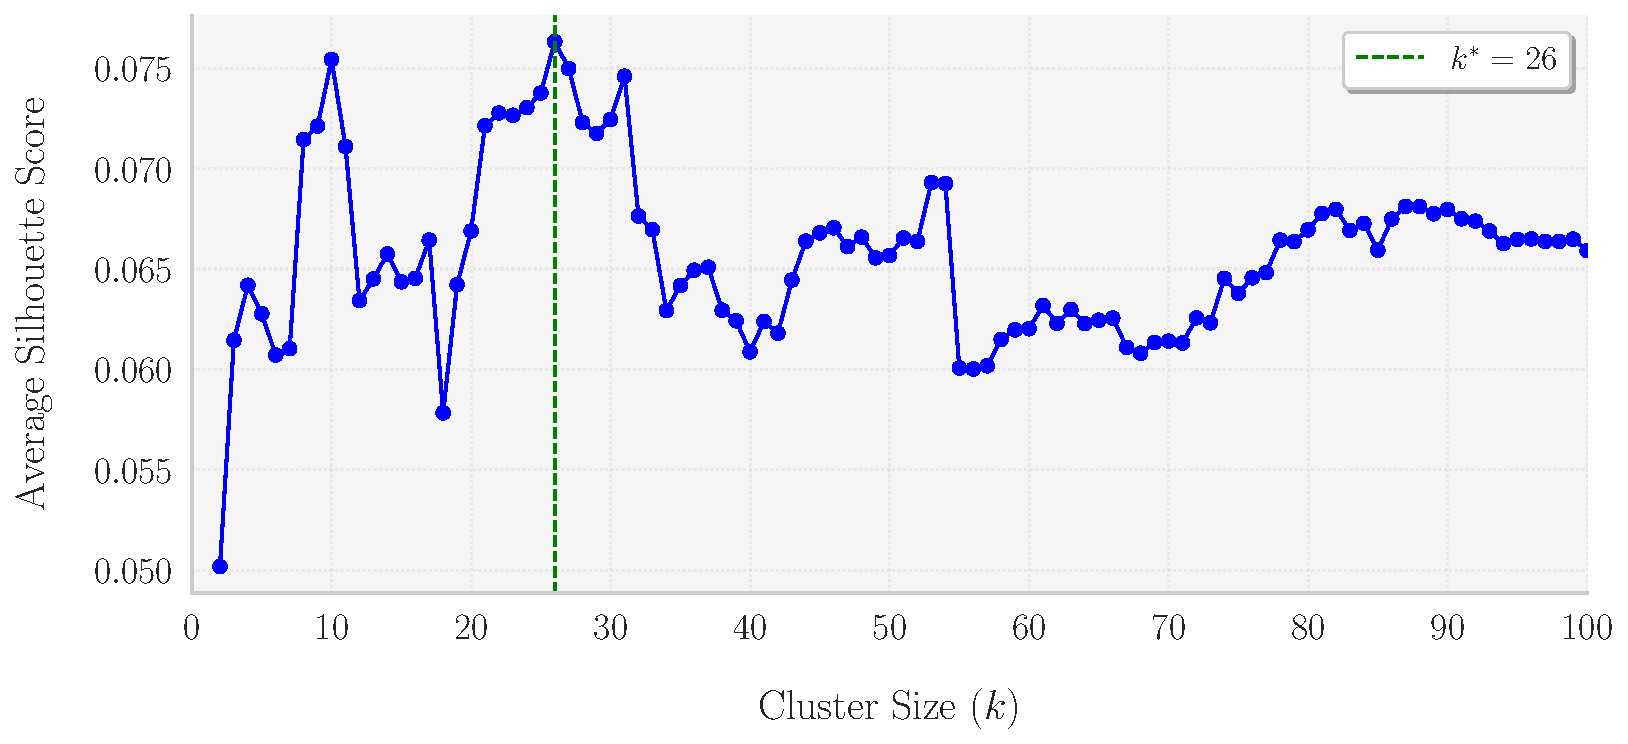
\includegraphics[scale=0.65]{/Users/jesusvillotamiranda/Library/CloudStorage/OneDrive-UniversidaddeLaRioja/CEMFI/Rest/__Second_year__/MasterThesis/__Output/KMeans_Clustering_Silhouette_Score.pdf}
\subcaption*{\textit{Note: This plot shows the average silhouette scores computed on $\D^{tr}$ over a grid of possible cluster sizes $\mbf k=\{2,...,100\}$. The maximizer $k^*=26$ is highlighted with a vertical dashed green line.}}
\label{fig:silhouette_score}
\end{figure}
%----------------------------------------------------




\mx
Given the optimal number of clusters $k^*$, we fit the KMeans algorithm on the training embeddings 
$\{\mbf e^i \mid i\in\D^{tr}\}$
%$\{ \mathbf{e}^1, \mathbf{e}^2, \ldots, \mathbf{e}^{N_{tr}} \}$
 to obtain the centroids $\{ \mathbf{c}^{tr}_1, \mathbf{c}^{tr}_2, \ldots, \mathbf{c}^{tr}_{k^*} \}$. Following \cref{alg:KMeans} (detailed in section A1 of the Appendix):
$$
\{ \mathbf{c}^{tr}_1, \mathbf{c}^{tr}_2, \ldots, \mathbf{c}^{tr}_{k^*} \} = \text{KMeans} ( \{ \mathbf{e}^1, \mathbf{e}^2, \ldots, \mathbf{e}^{N_{tr}} \}, k^* )
~.
$$

We then find the cluster associated to each embedding $\mathbf{e}^i$ in the validation set 
$\{\mbf e^i \mid i\in\D^{val}\}$ according to the centroids resulting from clustering the training data $\{\mbf c_1^{tr},..., \mbf c_{k^*}^{tr}\}$.
%$\{ \mathbf{e}^{N_{tr}+1}, \mathbf{e}^{N_{tr}+2}, \ldots, \mathbf{e}^{N_{tr}+N_{val}} \}$ to the nearest centroid $\mathbf{c}_g$. 
This allows us to obtain the clustering of the news articles in the validation sample
$$
\D_g^{val} = 
\3{ 
i\in \D^{val} 
\c g = \arg \min_{\ell\in\G} \|\mathbf{e}^i - \mathbf{c}^{tr}_{\ell}\|_{2}^2
}
\quad 
\forall g\in\G
.
$$

Similarly, by assigning each embedding $\mathbf{e}^i\in \{\mbf e^i \mid i\in\D^{test}\}$
 to the nearest centroid $\mathbf{c}^{tr}_g$, we obtain the clusters in the test set
$$
\D_g^{test} = 
\3{ 
i\in \D^{test}
\c g = \arg \min_{\ell\in\G} \|\mathbf{e}^i - \mathbf{c}^{tr}_{\ell}\|_{2}^2 
}
\quad 
\forall g\in\G
.
$$
%----------------------------------------------------

%
%%----------------------------------------------------
%\begin{figure}[H]
%  \centering
%  \caption{Distribution of articles through KMeans clusters}
%  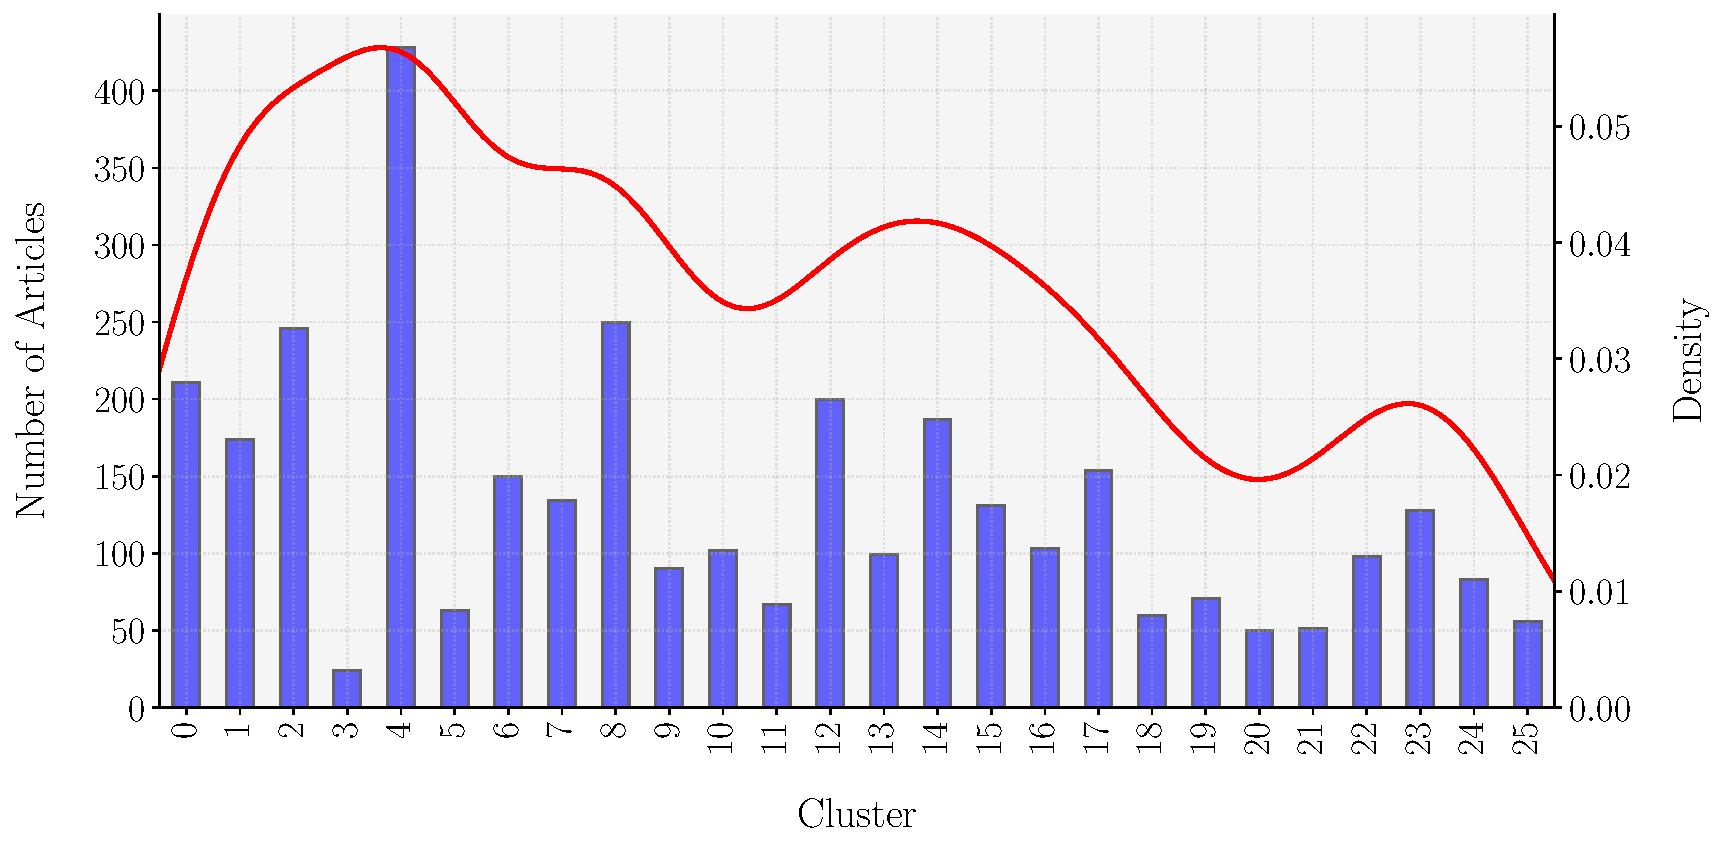
\includegraphics[scale=0.6]{/Users/jesusvillotamiranda/Library/CloudStorage/OneDrive-UniversidaddeLaRioja/CEMFI/Rest/__Second_year__/MasterThesis/__Output/KMeans_Cluster_Distribution.pdf}
%%  \caption{}
%\end{figure}
%%----------------------------------------------------
%
%
%%----------------------------------------------------
%\begin{figure}[h!]
%    \centering
%%    \caption{Distribution of articles through KMeans clusters across data splits}
%    \begin{subfigure}[b]{0.32\textwidth}
%        \centering
%        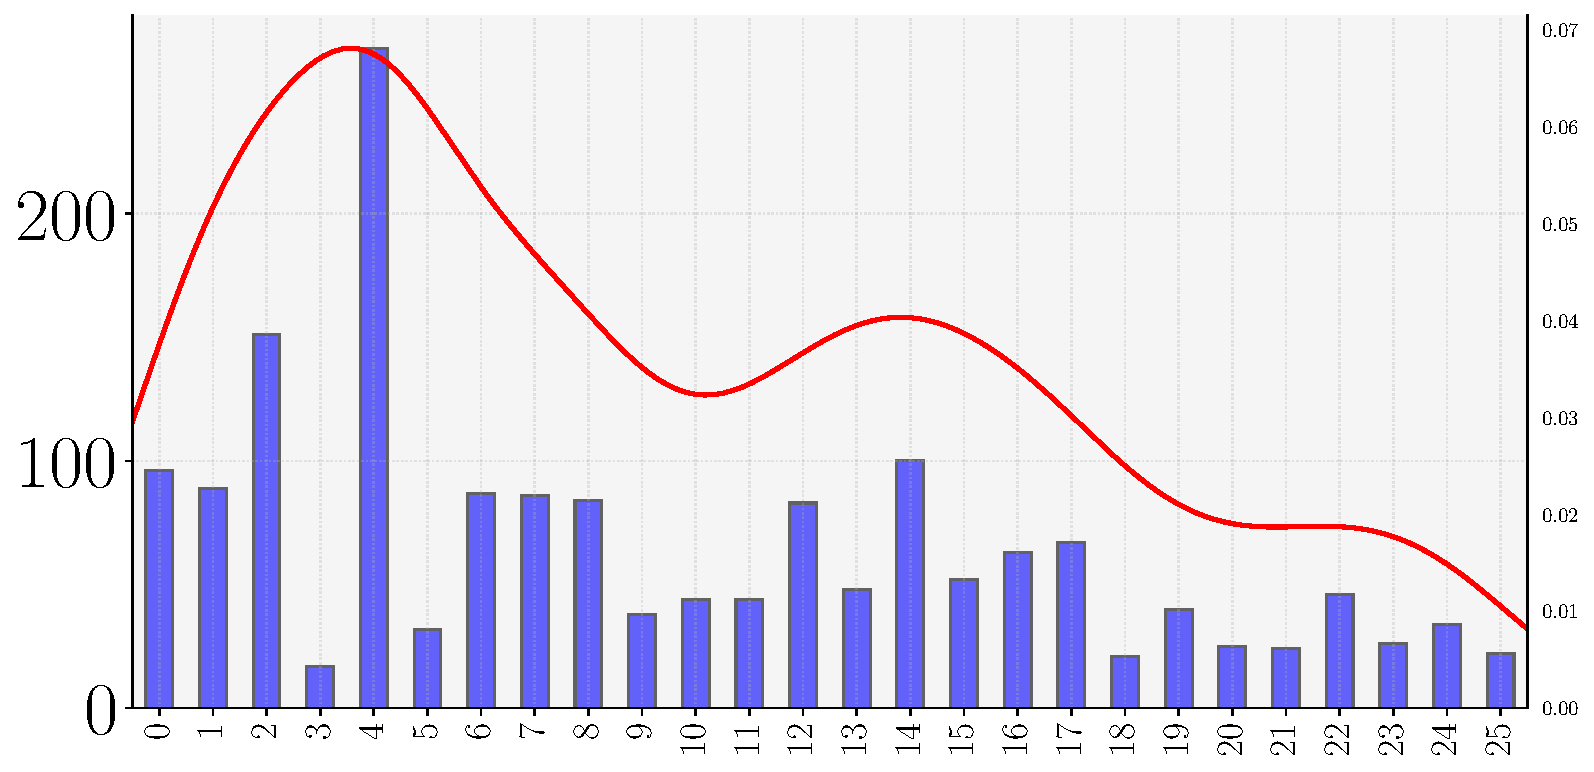
\includegraphics[width=\textwidth]{/Users/jesusvillotamiranda/Library/CloudStorage/OneDrive-UniversidaddeLaRioja/CEMFI/Rest/__Second_year__/MasterThesis/__Output/KMeans_Cluster_Distribution_Train.pdf}
%        \caption{Training data ($D^{tr}$)}
%        \label{fig:plot1}
%    \end{subfigure}
%    \begin{subfigure}[b]{0.32\textwidth}
%        \centering
%        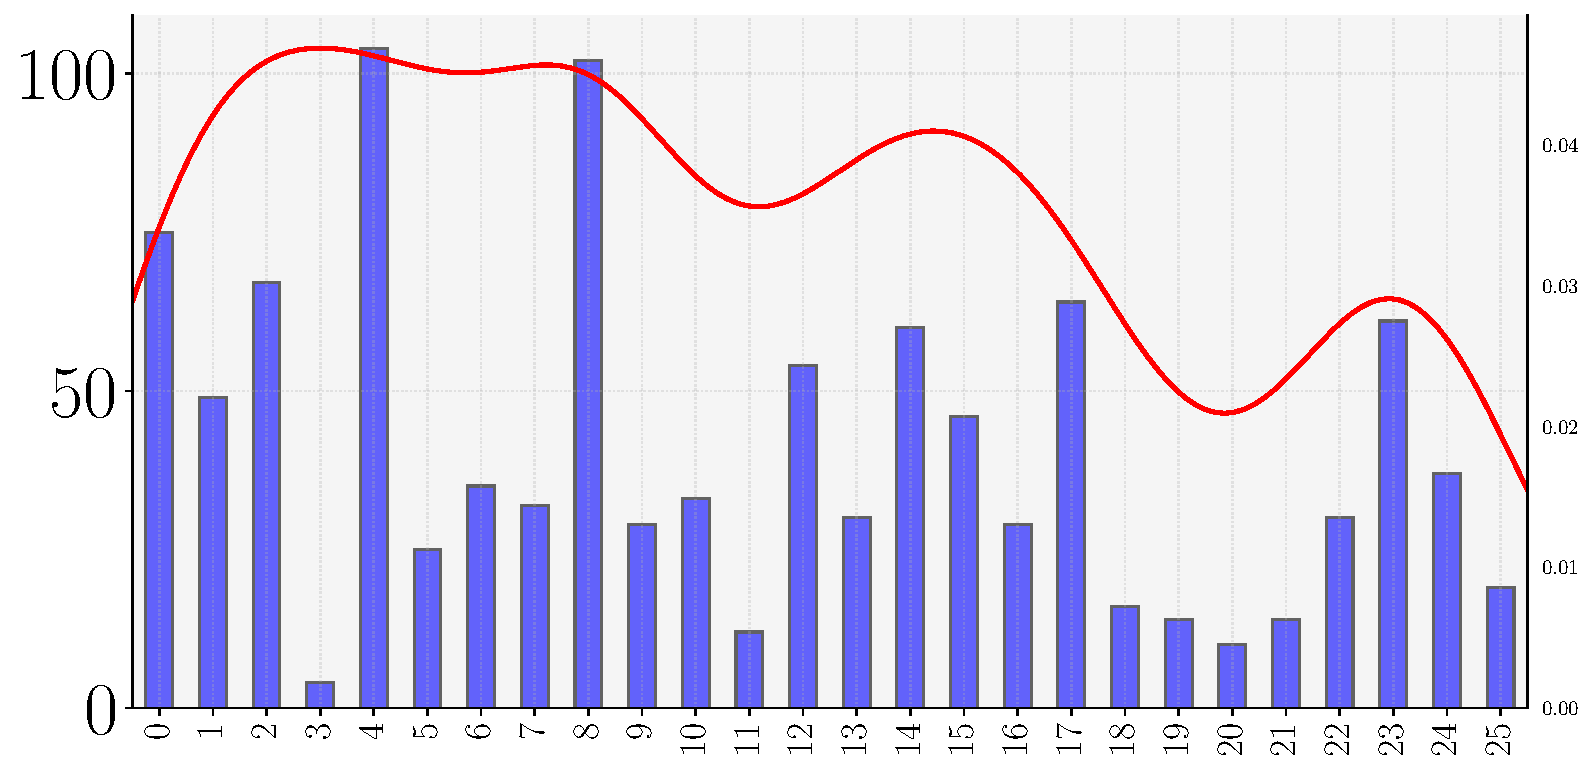
\includegraphics[width=\textwidth]{/Users/jesusvillotamiranda/Library/CloudStorage/OneDrive-UniversidaddeLaRioja/CEMFI/Rest/__Second_year__/MasterThesis/__Output/KMeans_Cluster_Distribution_Validation.pdf}
%        \caption{Validation data ($D^{val}$)}
%        \label{fig:plot2}
%    \end{subfigure}
%    \begin{subfigure}[b]{0.32\textwidth}
%        \centering
%        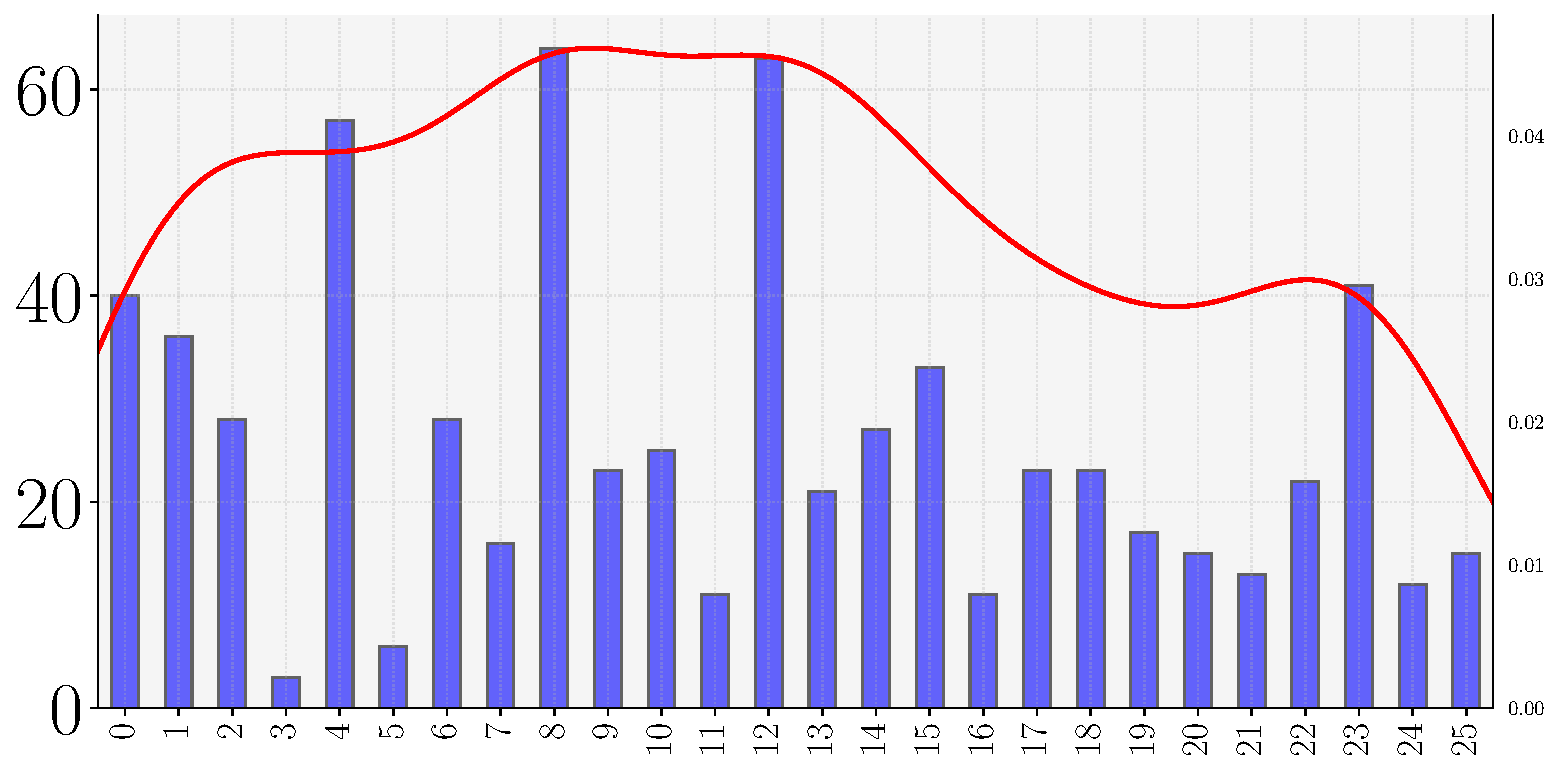
\includegraphics[width=\textwidth]{/Users/jesusvillotamiranda/Library/CloudStorage/OneDrive-UniversidaddeLaRioja/CEMFI/Rest/__Second_year__/MasterThesis/__Output/KMeans_Cluster_Distribution_Test.pdf}
%        \caption{Test data ($D^{test}$)}
%        \label{fig:plot3}
%    \end{subfigure}
%    \label{fig:three_plots}
%\end{figure}
%%----------------------------------------------------

%----------------------------------------------------
\begin{figure}[H]
    \centering
    \caption{Distribution of articles through KMeans clusters}
    
    % Upper plot
    \begin{subfigure}[b]{\textwidth}
        \caption{All data ($\mathcal D$)}
        \centering
        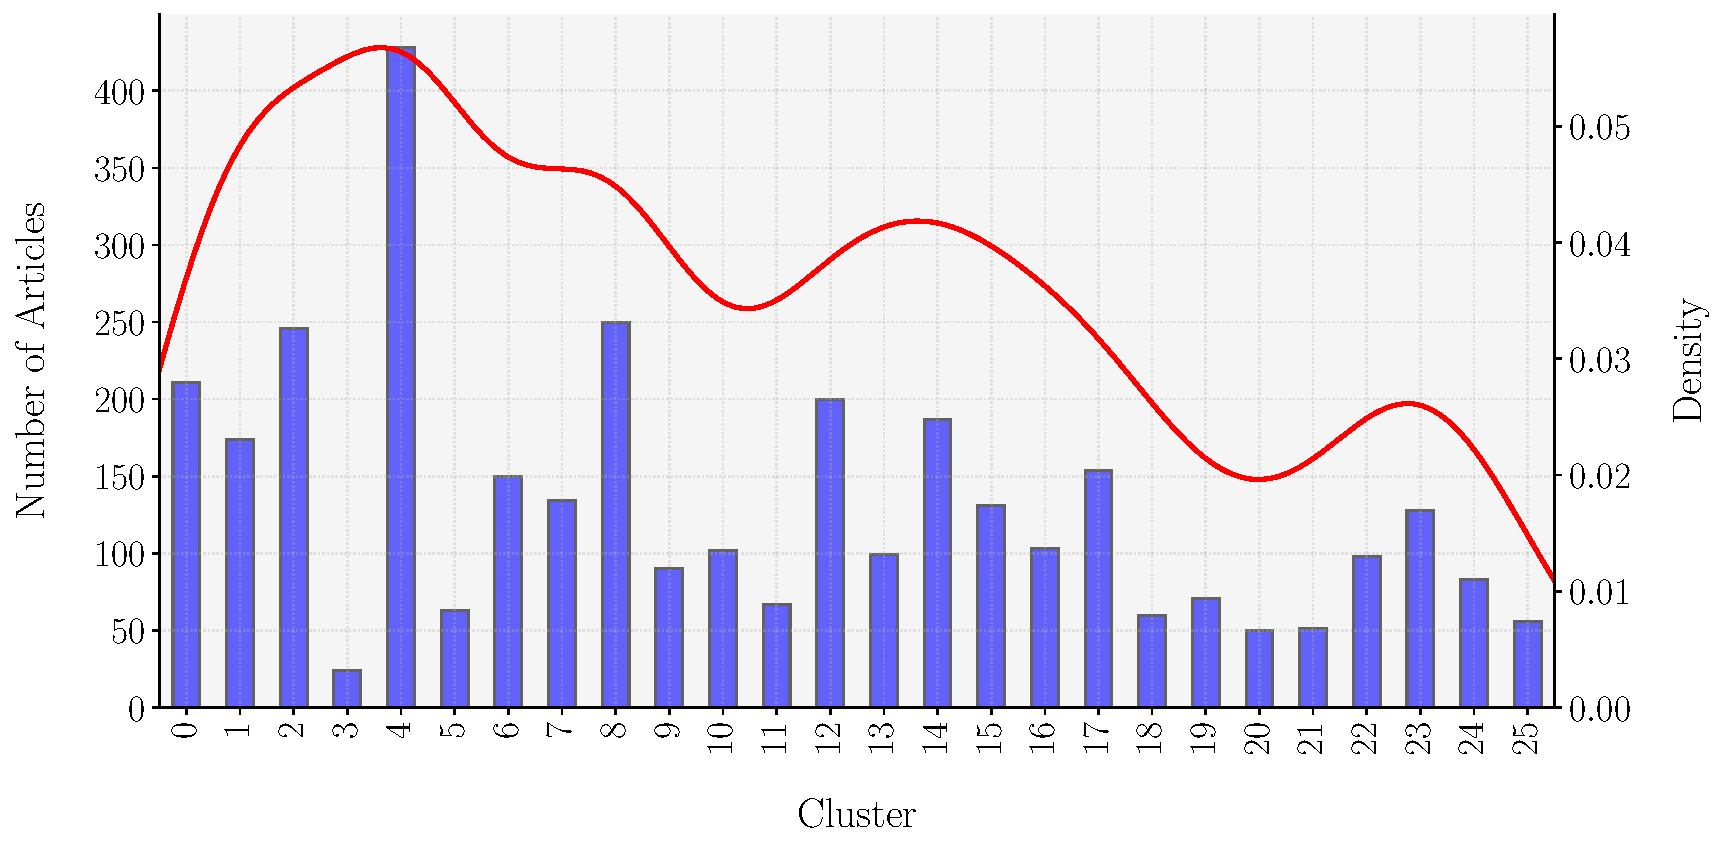
\includegraphics[scale=0.45]{/Users/jesusvillotamiranda/Library/CloudStorage/OneDrive-UniversidaddeLaRioja/CEMFI/Rest/__Second_year__/MasterThesis/__Output/KMeans_Cluster_Distribution.pdf}
        \label{fig:all_data}
    \end{subfigure}

    % Lower plots
    \begin{subfigure}[b]{0.32\textwidth}
        \caption{Training data ($\D^{tr}$)}
        \centering
        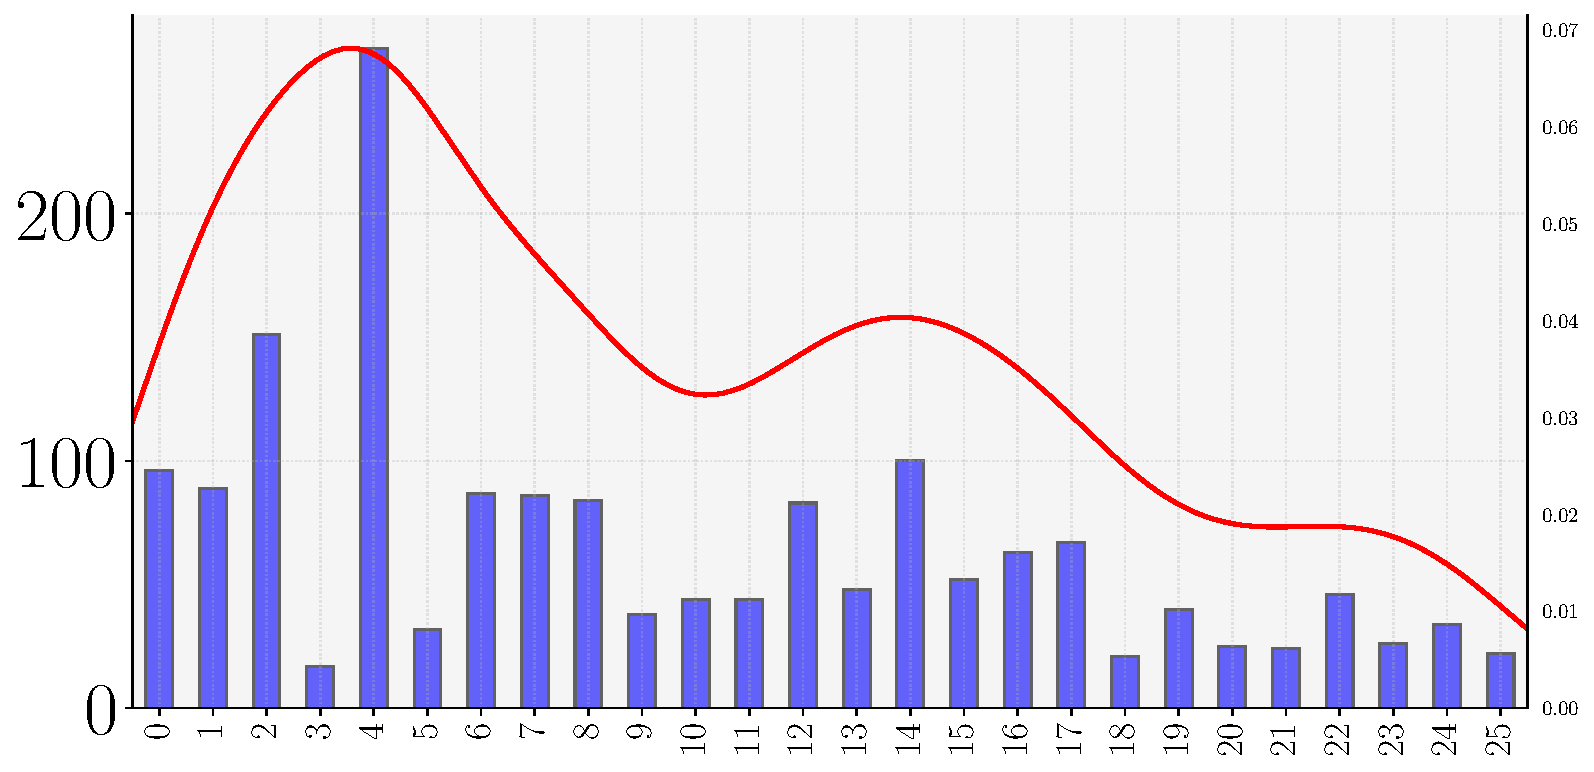
\includegraphics[width=\textwidth]{/Users/jesusvillotamiranda/Library/CloudStorage/OneDrive-UniversidaddeLaRioja/CEMFI/Rest/__Second_year__/MasterThesis/__Output/KMeans_Cluster_Distribution_Train.pdf}
        \label{fig:train_data}
    \end{subfigure}
    \begin{subfigure}[b]{0.32\textwidth}
        \caption{Validation data ($\D^{val}$)}
        \centering
        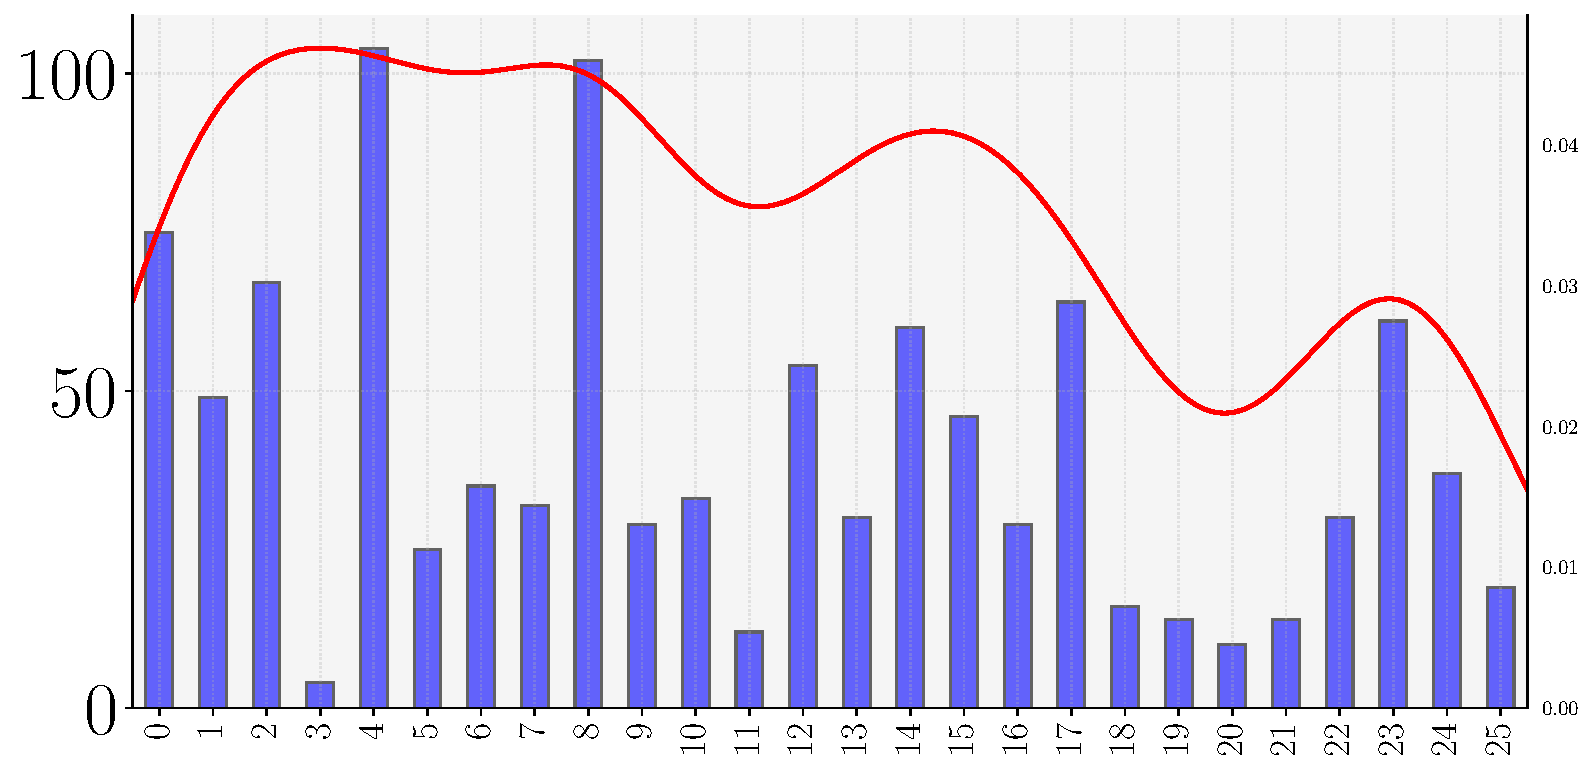
\includegraphics[width=\textwidth]{/Users/jesusvillotamiranda/Library/CloudStorage/OneDrive-UniversidaddeLaRioja/CEMFI/Rest/__Second_year__/MasterThesis/__Output/KMeans_Cluster_Distribution_Validation.pdf}
        \label{fig:val_data}
    \end{subfigure}
    \begin{subfigure}[b]{0.32\textwidth}
        \caption{Test data ($\D^{test}$)}
        \centering
        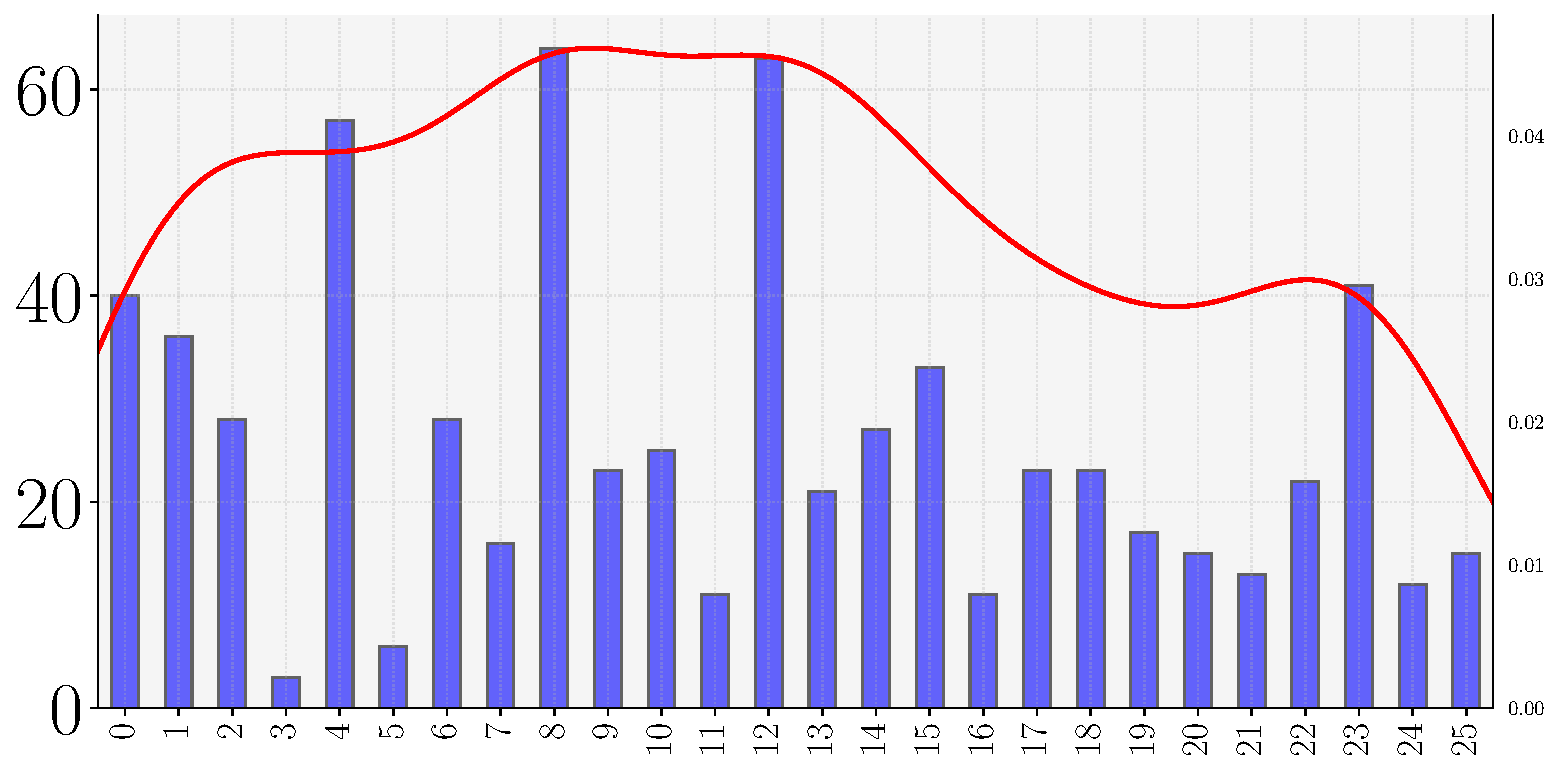
\includegraphics[width=\textwidth]{/Users/jesusvillotamiranda/Library/CloudStorage/OneDrive-UniversidaddeLaRioja/CEMFI/Rest/__Second_year__/MasterThesis/__Output/KMeans_Cluster_Distribution_Test.pdf}
        \label{fig:test_data}
    \end{subfigure}
    \label{fig:combined_plots}
\subcaption*{\textit{Note: The upper plot shows the distribution of all the articles $i\in \mathcal D$ through the KMeans clusters, while the lower plots show the distributions for the training ($\D^{tr}$), validation ($\D^{val}$), and test ($\D^{test}$) articles respectively.}}
\end{figure}
%----------------------------------------------------

As we can see, the distribution of articles in the whole sample ($\D$) is fairly homogenous across the 26 clusters, with each cluster containing between 50 and 250 articles on average. The notable exceptions are cluster 3, which contains only 24 articles, and cluster 4, which concentrates 428 articles. However, the distribution profile is not consistent over data splits, which indicates that this classification procedure is unstable over time.

\mx 
Although not directly interpretable, by looking at the articles pooled in a certain cluster, we can provide some intuition of what it represents. In most cases, each cluster contains articles involving a firm or set of firms in the same sector. For example, cluster 3 pools articles about Telef�nica and Cellnex (telecoms), cluster 4 contains articles about CaixaBank, cluster 9 concentrates articles about Repsol, cluster 12 about Iberdrola, cluster 15 gathers articles on Infrastructure (led by ACS and Acciona) and so on.

\mx 
However, there are some exceptions to this general rule, for example, cluster 0 is a \qquote{miscellanous} cluster:
% with no clear pattern: 
 it covers articles about different firms with no apparent relation between them. Another example is cluster 1, which pools articles related to the quarterly or semiannual publication of results by different firms. In \cref{tab:KMeans_Articles_3_English} of the Appendix we provide a sample of 3 articles for each cluster and propose a name for each one based on the articles they pool.


%Even though the interpretation of the clusters is not always clear, we can try to provide a general topic to each of them based on the type of articles that they contain.


%
%\red{Explain what each cluster means and provide examples of articles in each of the clusters}
%
%
%Despite a few exceptions, the distribution of articles by cluster is fairly homogeneous, with each cluster containg between 100 and 250 articles on average. The notable exceptions are clusters 3, with only \red{20?: CHECK} articles, and cluster 4, with over 400 articles. 
%
%




%%%%%%%%%%%%%%%%%%%%%%%%%%%%%%%%%%%%%%%%%%%%%%%%%%%%%
%%%%%%%%%%%	   DELETE BELOW   %%%%%%%%%%%%%%%%%%%%%%%
%%%%%%%%%%%%%%%%%%%%%%%%%%%%%%%%%%%%%%%%%%%%%%%%%%%%%

%\subsection{Notation for trading days}
%To facilitate the understanding and implementation of our trading strategy, we introduce a clear and systematic notation for handling trading days. We define 
%%the ordered set trading days as 
%$\tilde{\mathfrak{d}}=\3{\tilde{\mathfrak{d}}_1, \tilde{\mathfrak{d}}_2, \ldots}$, representing an ordered sequence of trading days. To map a specific trading day $\tilde{d} \in \tilde{\mathfrak{d}}$ to its position within this sequence, we define the Index function $\mathbb{I}_{\tilde{\mathfrak{d}}}: \tilde{d} \in \tilde{\mathfrak{d}} \longrightarrow \{1, 2, \ldots, |\tilde{\mathfrak{d}}|\}$. For any given trading day $\tilde{d} = \tilde{d}_k \in \tilde{\mathfrak{d}}$, the Index function $\mathbb{I}_{\tilde{\mathfrak{d}}}(\tilde{d})$ returns its position $k$. Conversely, the function $\mathbb{D}_{\tilde{\mathfrak{d}}}(k)$ retrieves the trading day corresponding to a given index $k$, ensuring the ordered structure is maintained. Additionally, for any date $d$ not in $\tilde{\mathfrak{d}}$, the operator $\Lambda(d)$ returns the next closest trading day within $\tilde{\mathfrak{d}}$. This systematic notation is crucial for accurately defining trading windows, such as the market model window $[\mathbb{D}_{\tilde{\mathfrak{d}}}(\mathbb{I}_{\tilde{\mathfrak{d}}}(\tilde{d}_0^i) - \widetilde{w}_b - \widetilde{w}_m), \mathbb{D}_{\tilde{\mathfrak{d}}}(\mathbb{I}_{\tilde{\mathfrak{d}}}(\tilde{d}_0^i) - \widetilde{w}_b)]$, ensuring both start and end points are valid trading days. This notation aids in defining the trading rule $T R_{L, \theta}$ and the portfolio $\mathcal{P}$ precisely, enhancing the robustness and clarity of our strategy's implementation.
%
%
%\textbf{Market Model Window Definition}
%
%For each unique pair $(i, j) \in \mathcal{B}$, we fit a market model on some window
%$\mathcal{M}:=$
% before the news publication date $\tilde{d}_0^i$. The market model window is defined using the above notation to ensure start and end points are both trading days:
%$$
%r_{\tilde{d}}^j = \alpha^{(i, j)} + \beta^{(i, j)} r_{\tilde{d}}^M + \epsilon_{\tilde{d}}^{(i, j)} \quad \text{for } \tilde{d} \in 
%\left[ 
%\mathbb{D}_{\tilde{\mathfrak{d}}} \left( \mathbb{I}_{\tilde{\mathfrak{d}}} (\tilde{d}_0^i) - \widetilde{w}_b - \widetilde{w}_m \right), \mathbb{D}_{\tilde{\mathfrak{d}}} 
%\left( \mathbb{I}_{\tilde{\mathfrak{d}}} (\tilde{d}_0^i) - \widetilde{w}_b 
%\right) 
%\right],
%$$
%where $\widetilde{w}_b$ denotes the buffer window (10 trading days) and $\widetilde{w}_m$ denotes the market model window (100 trading days).
%
%\textbf{Trading Rule and Portfolio Definition}
%
%For a given selection of clusters $\mathcal{G}_\theta^{+}$ and $\mathcal{G}_\theta^{-}$, we launch trades with a holding period of $L$ trading days. The trading rule $T R_{L, \theta}\langle(i, j), \tilde{d}\rangle$ for a pair $(i, j) \in \mathcal{B}$ at trading day $\tilde{d}$ is defined as follows.
%
%In this context, a portfolio is a collection of positions taken in firm's stocks according to $T R_{L, \theta}\langle(i, j), \tilde{d}\rangle$. In other words, it is the set of all $\langle(i, j), \tilde{d}\rangle$ for which a trade is executed:
%\[
%\mathcal{P}: = \3{\langle(i, j), \tilde{d}\rangle \mid (i, j) \in \mathcal{B} \wedge \tilde{d} \in \tilde{\mathfrak{d}} \wedge T R_{L, \theta}\langle(i, j), \tilde{d}\rangle \neq 0 }.
%\]
%
%The return of the portfolio on trading date $\tilde{d}$, denoted as $r_{\tilde{d}}^{\mathcal{P}}$, is the average return of the individual positions:
%\[
%r_{\tilde{d}}^{\mathcal{P}} = \frac{1}{|\mathcal{P}_{\tilde{d}}|} \sum_{\langle(i, j), \tilde{d}\rangle \in \mathcal{P}_{\tilde{d}}} AR_{\tilde{d}}^{(i, j)},
%\]
%where $\mathcal{P}_{\tilde{d}} = \3{\langle(i, j), \tilde{d}\rangle \in \mathcal{P} \mid \tilde{d} - L + 1 \leq \tilde{d} \leq \tilde{d} }$ represents the set of open positions on trading day $\tilde{d}$.

%%%%%%%%%%%%%%%%%%%%%%%%%%%%%%%%%%%%%%%%%%%%%%%%%%%%%
%%%%%%%%%%%	   DELETE ABOVE   %%%%%%%%%%%%%%%%%%%%%%%
%%%%%%%%%%%%%%%%%%%%%%%%%%%%%%%%%%%%%%%%%%%%%%%%%%%%%




%----------------------------------------------------
\subsection{Beta-neutral positions on every $(i,j)\in\mathcal B$}
Since we are interested in the individual effect of an article $i\in\D$ in each of the affected firms $j\in\F^i$, we define the set
$
\mathcal{B}:=\3{(i,j) \mid i\in \D ~\wedge~j\in \F^i }
$, where $\abs{\mathcal{B}}=3410>\abs{\D}=2613$. 
We then fit a market model to each unique pair $(i,j)\in \mathcal{B}$
%consisting of a firm $j\in\F^i$ affected by article $i$ 
on some window of time $\mathcal{M}^i\subset \tilde{\mathfrak{d}}$ before the effective treatment day: 
\footnote{To rigorously define $\mathcal M^i$, we need to work with the index and inverse index functions. 
\begin{itemize}
  \item \textbf{Index Function}. 
Given a finite ordered set $\mathcal{Z}=\left\{z_1, z_2, \ldots, z_n\right\}$, the index function 
$\mathbb{I}_{\mathcal{Z}}: \mathcal{Z} \rightarrow\{1,2, \ldots,|\mathcal{Z}|\}$
%$\mathbb{I}_{\mathcal{Z}}(z)$
 maps an element $z\in\Z$ to its position in the ordered set $\mathcal{Z}$. Formally:
$
\mathbb{I}_{\mathcal{Z}}(z_{\ell})=\ell 
%\quad \text { if and only if } \quad z=z_{\ell} 
~ \text { for } ~ \ell \in\{1,2, \ldots,|\mathcal{Z}|\}
.
$
%where $z_{\ell}$ denotes the ${\ell}$-th element of the ordered set $\mathcal{Z}$.

\item \textbf{Inverse Index Function}. 
The inverse index function 
$\mathbb{I}_{\mathcal{Z}}^{-1}:\{1,2, \ldots,|\mathcal{Z}|\} \rightarrow \mathcal{Z}$
%$\mathbb{I}_{\mathcal{Z}}^{-1}({\ell})$
 retrieves the element $z \in \mathcal{Z}$ corresponding to a given index ${\ell}$.
Formally:
$
\mathbb{I}_{\mathcal{Z}}^{-1}({\ell})=z_{\ell} ~\text { for } ~{\ell} \in\{1,2, \ldots,|\mathcal{Z}|\}
.$
\end{itemize}
For the market model window, we use $\mathbb{I}_{\tilde{\mathfrak{d}}}$ and $\mathbb{I}^{-1}_{\tilde{\mathfrak{d}}} $ applied to the set of trading days $\tilde{\mathfrak d}$. Namely:
$$
\mathcal{M}^i := 
\3{
d\in \tilde{\mathfrak{d}}
\c 
\mathbb{I}^{-1}_{\tilde{\mathfrak{d}}} 
\1{
\mathbb{I}_{\tilde{\mathfrak{d}}} (\tilde{d}_0^i) - {w}_b - {w}_m 
}
\leq d \leq 
\mathbb{I}^{-1}_{\tilde{\mathfrak{d}}} 
\1{ 
\mathbb{I}_{\tilde{\mathfrak{d}}} (\tilde{d}_0^i) - {w}_b 
}
}
,
$$
with a buffer of ${w}_b=10$ trading days before the effective treatment date, and a market model window length of ${w}_m=100$ trading days.



}
%----------------------------------------------------
$$
r_{d}^{j} = \alpha^{(i,j)} + \beta^{(i,j)} r_{d}^M + \epsilon_{ d}^{(i,j)} 
\qquad  
%\t{for}
%~
%\qquad
\forall d \in \mathcal{M}^i
,
$$
%\begin{align*}
%r_{\tilde d}^{j} = \alpha^{(i,j)} + \beta^{(i,j)} r_{\tilde d}^M + \epsilon_{\tilde d}^{(i,j)} 
%\qquad  
%\t{for}
%~
%%\qquad
%\tilde d \in 
%\5{
%\tilde d_0^i - \widetilde{w}_b - \widetilde{w}_m
%~,~
%\tilde d_0^i - \widetilde{w}_b
%}
%,
%\end{align*}
where 
$r_{d}^{j}$ denotes the return of firm $j$ at trading day $d$ in excess of the risk-free asset, which we take to be the daily euro short-term rate (\texttt{\euro STR}),
and 
$r_{d}^M$ denotes the excess return of the market (IBEX-35).  
%----------------------------------------------------
These returns are obtained from the adjusted close price, which corrects the price evolution for corporate actions such as dividends, stock splits, and new stock issuance.\footnote{
The adjusted close price ensures that the returns reflect the true economic gains or losses for an investor holding the stock. 
%
Formally, the return of firm $j$ between two trading days $d_1, d_2\in \tilde{\mathfrak{d}}$ is computed as:
$
r_{d_1:d_2}^{j} = 
%\frac{
(
p_{d_2}^{j,\text{adj}} - p_{d_1}^{j,\text{adj}}
%}{
)/(
p_{d_1}^{j,\text{adj}}
)
%},
$
where $p_{d}^{j,\text{adj}}$ is the adjusted close price of firm $j$ at trading day $d$.
}
%----------------------------------------------------

\mx 
%----------------------------------------------------
The notation overload in the regression coefficients $(\alpha^{(i,j)},\beta^{(i,j)})$ emphasizes the fact that $\alpha$ and $\beta$ are specific to each pair $(i,j)\in\mathcal B$ since the market model is computed for each firm $j\in\F_{\t{IBEX-35}}$ on some specific window of time $\mathcal{M}^i$, which is particular to each article $i\in\D$.
%----------------------------------------------------

\mx 
The reason why we fit a market model to each $(i,j)\in\mathcal B$ is to then apply 
a market-neutral strategy. This is an investment approach designed to minimize or eliminate exposure to overall market movements, isolating the performance of a specific firm. 
%The primary goal is to achieve positive returns regardless of the market's direction (up or down). 
In particular, we employ a beta-neutral strategy by buying one unit of firm $j$'s stock and shorting $\beta^{(i,j)}$ units of the market index (i.e.: an ETF replicating the IBEX-35). 

%where $\beta^{(i,j)}$ is the sensitivity of the firm's stock to the market. 

% This approach allows us to isolate the impact of news articles on individual stock performance without the confounding influence of market-wide movements.

%This approach neutralizes the impact of broad market movements, allowing us to focus on the abnormal returns generated by specific news events. 
%This beta-neutral strategy isolate the impact of news articles on individual stock performance without the confounding influence of market-wide movements.


%\mx 
%Based on the estimates $( \alpha^{(i,j)},  \beta^{(i,j)})$, we apply a market-neutral strategy, which is an investment approach designed to minimize or eliminate exposure to overall market movements, isolating the performance of firm $j$. The primary goal is to achieve positive returns regardless of the market's direction (up or down). In this strategy, long positions are taken in firms expected to outperform the market, and short positions are taken in firms expected to underperform. 

%The beta-neutral aspect involves adjusting the portfolio so that the weighted average beta is zero, meaning the portfolio's value should not be affected by market movements. This reduces market risk and focuses on the performance of selected securities. By employing a beta-neutral strategy in this thesis, we aim to isolate the impact of news articles on individual stock performance without the confounding influence of market-wide movements.
%----------------------------------------------------
\mx
This hedged position harvests the idiosyncratic returns from the market model and it only makes sense when firm $j$'s returns are expected to outperform or underperform the market.\footnote{
For expected underperformance of firm $j$, reverse the beta neutral positions: 
sell one unit of firm $j$ and buy $\beta^{(i,j)}$ units of the market index. However, note that this will be handled later by a Trading Rule $(TR)$.
%Note that in the case of expected underperformance of firm $j$, the beta neutral positions should be reversed: sell one unit of firm $j$ and buy $\beta^{(i,j)}$ units of the market index. But for now, there is no need to be concerned with this: the ultimate construction of the positions will be managed by the later introduced Trading Rule $(TR)$.
\mx 
}
The position delivers abnormal returns $AR^{(i,j)}_{d}$ at some trading day $d\geq \tilde{d}_0^i$ given by
%
%Based on the estimates $( \alpha^{(i,j)},  \beta^{(i,j)})$, we compute the returns of a position that buys firm $j$'s stock and sells $ \beta^{(i,j)}$ times the market (by entering into a short position in an ETF that replicates the IBEX-35 Index). This hedged position delivers abnormal returns at trading date $\tilde d$ given by
\begin{align*}
r_{d}^j -  \beta^{(i,j)} r_{d}^M = \alpha^{(i,j)} + \epsilon_{d}^{(i,j)} =: AR^{(i,j)}_{d}
.
\end{align*}
%----------------------------------------------------
The position is taken at the effective treatment date $\tilde d_0^i$ and is maintained over a holding window $\mathcal H^i \subset \tilde{\mathfrak{d}}$ consisting of $L\in\mathbb{N}$ trading days after $\tilde d_0^i$, where $L$ is set to 4 trading days.\footnote{  
The holding period of the position is defined as 
$
\mathcal H^i:=
\3{
d \in \tilde{\mathfrak{d}}
\c 
\tilde{d}_0^i
\leq d \leq 
\mathbb{I}^{-1}_{\tilde{\mathfrak{d}}}\1{\mathbb{I}_{\tilde{\mathfrak{d}}}(\tilde d_0^i)+L}}
%\mathbb{D}_{\tilde{\mathfrak{d}}}\1{\mathbb{I}_{\tilde{\mathfrak{d}}}(\tilde d_0^i)+L}}
$}
%----------------------------------------------------
The justification for this choice of $L$ is made in section A.2 of the Appendix. 

%----------------------------------------------------
\mx 

After having held the beta-neutral position over the holding period $\mathcal H^i$, we obtain a time series of abnormal returns $\{AR_{d}^{(i,j)}\}_{d\in\mathcal H^i}$ from where we can obtain the usual performance metrics. First, the average daily log returns are obtained as
$$
\mu^{(i,j)} = \frac{1}{{{L}}+1} 
%\sum_{d=\tilde d_0^i }^{\tilde d_0^i + {{L}}} 
\sum_{d\in \mathcal H^i}
\ln\4{1+AR_d^{(i,j)}}
~,
$$
%$
%\mu_{{{L}}}^{(i,j)}
%=
%\1{1+CAR_{{{L}}}^{(i,j)}}^{1/({{L}}+1)}-1,
%$
Then, the standard deviation is given by
$$
\sigma^{(i,j)}
=
\sqrt{
\frac{1}{{{L}}}
\sum_{d\in \mathcal H^i}
%\sum_{d=\tilde d_0^i }^{\tilde d_0^i + {{L}}} 
[
\ln(1+AR_d^{(i,j)}) - \mu^{(i,j)}
]
^2}
~.
$$

\mx 
And finally, the annualized Sharpe Ratio can be obtained by scaling the daily Sharpe Ratio by the square root of ${252}$, which are the typical number of trading days in a year according to the Spanish calendar. 
%.  $\sqrt{|\tilde{\mathfrak d}_y|}$
%$
%\sigma_{{{L}}}^{(i,j)}
%= \sqrt{\frac{1}{{{L}}} \sum_{d=\tilde d_0^i}^{\tilde d_0^i + {{L}}} 
%\1{ AR_d^{(i,j)} -\mu_{{{L}}}^{(i,j)} }^2}
%$
$$
SR^{(i,j)} =
\sqrt{252}~
\frac{
\mu^{(i,j)}
}{
\sigma^{(i,j)}
}
%\sqrt{|\tilde{\mathfrak d}_y|}
~.
$$
%%%%%%%%%%%%%%%%%%%%%%%%%%%%%%%%%%%%%%%%%%%%%%%%%%%%%
\subsection{Optimal Cluster Selection}
%%%%%%%%%%%%%%%%%%%%%%%%%%%%%%%%%%%%%%%%%%%%%%%%%%%%%

After taking beta-neutral positions on each pair $(i,j)\in\mathcal B$ and holding them over some window $\mathcal H^i$, we can obtain a measure of how profitable the positions are on average for articles that belong to the same cluster $g\in\mathcal G$. For this purpose, let $\mathcal{B}_g$ denote the set of all article and firm pairs such that the article belongs to some cluster $g\in\mathcal G$. 
$$
\mathcal{B}_g:= \{(i,j) \mid (i,j)\in\mathcal{B} ~\wedge~ i \in \D_g \}
.
$$
The average Sharpe Ratio associated to each cluster is
$$
\overline{S R}_g=\frac{1}{\left|\mathcal{B}_g\right|} \sum_{(i,j) \in \mathcal{B}_g} S R^{(i,j)}
,
$$
and it provides a measure of the performance of the beta-neutral positions in each cluster. 
The distribution of cluster-average Sharpe Ratios across the different clusters is plotted in \cref{fig:KMeans_distr_avg_SR}. In the validation set, they are centered at 0, but we observe some outliers with unusually low and high average $SR$. On the other hand, the distributions in the train and test data are slightly skewed to the right and show no presence of substantial outliers.

%----------------------------------------------------
\begin{figure}[H]
  \centering
  \caption{Distribution  of Cluster-Average Sharpe Ratios $(\overline{SR}_g)$ by Split}
  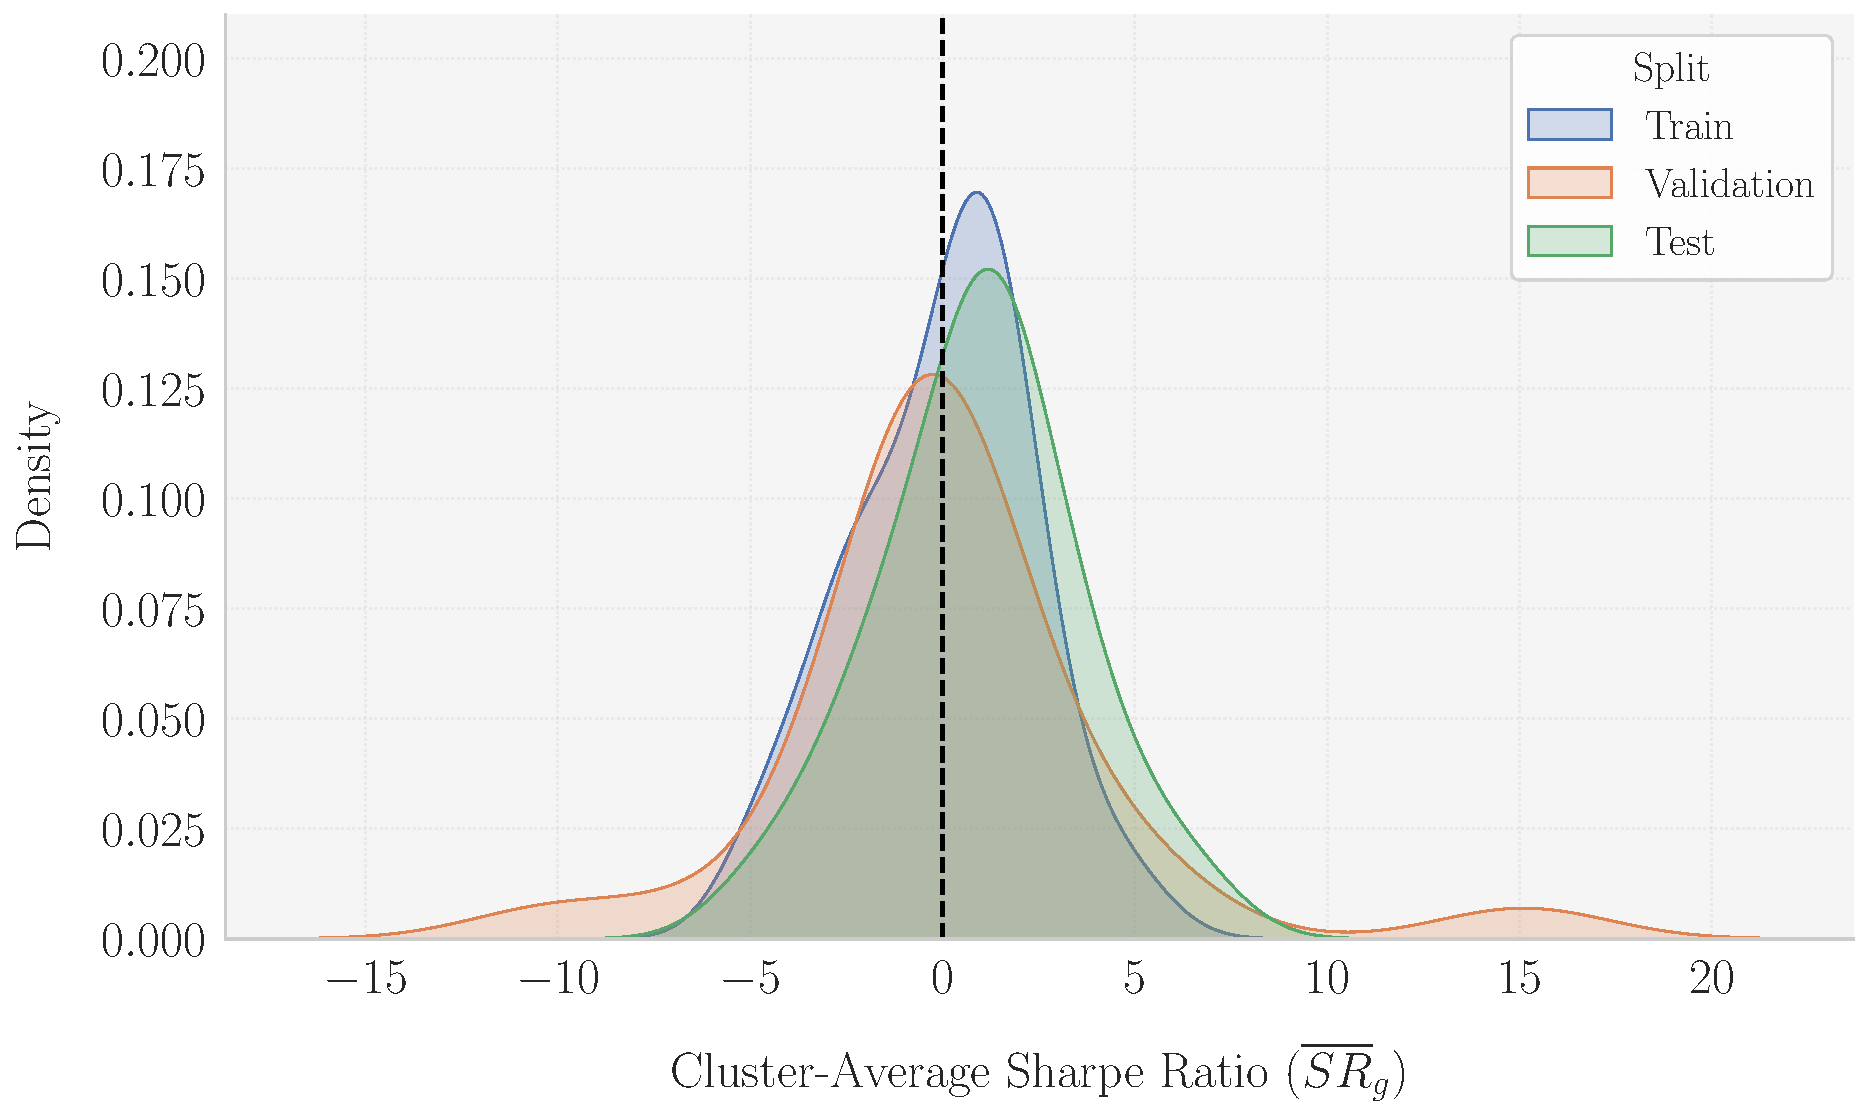
\includegraphics[scale=0.45]{/Users/jesusvillotamiranda/Library/CloudStorage/OneDrive-UniversidaddeLaRioja/CEMFI/Rest/__Second_year__/MasterThesis/__Output/KMeans_Cluster-Avg_SR_Distribution.pdf}
\label{fig:KMeans_distr_avg_SR}
\end{figure}
%----------------------------------------------------

\mx
The goal is to now design an algorithm that exploits this information to select the best clusters for the trading strategy. In the remainder of this section, we propose two algorithms. First, an algorithm developed on validation data that will select the clusters maximizing the performance for that split (\qquote{greedy}), and second, an algorithm that will exploit the information from both, training and validation data (higher information set), and whose objective will be to select the most stable clusters among both splits (\qquote{stable}). 


%----------------------------------------------------
%By exploiting the Sharpe Ratios of the beta-neutral positions, we can obtain a simple measure of the profitability of each cluster. In particular, by averaging the annualized Sharpe Ratios of the positions associated to articles that belong to the same cluster. 
%%----------------------------------------------------
%We can then average the annualized Sharpe Ratios of the positions associated to articles that belong to the same cluster. 
%%That is, for each cluster $g$, we compute the average Sharpe Ratio by averaging the Sharpe Ratios of all pairs $(i,j)$ where $i$ belongs to cluster $g$. 
%%--------------- OPTION 1---------------------
%Define $\mathcal{B}_g$ as the set of all pairs $(i,j)\in\mathcal{B}$ such that article $i$ belongs to cluster $g$
%$$
%\mathcal{B}_g:= \{(i,j) \mid (i,j)\in\mathcal{B} ~\wedge~ i \in \D_g \}
%.
%$$
%%--------------- OPTION 2--------------------------- 
%%Formally, let $\mathcal{B}_g$ be the set of all pairs $(i,j)$ such that article $i$ belongs to cluster $g$. 
%%$$\mathcal{B}_g := \{(i,j) \mid  \mbf e^i \in \D_g \}$$
%%----------------------------------------------------
%The average Sharpe Ratio for cluster $g$, denoted as $\overline{S R}_g$, is given by:
%$$
%\overline{S R}_g=\frac{1}{\left|\mathcal{B}_g\right|} \sum_{(i,j) \in \mathcal{B}_g} S R_{{{L}}}^{(i,j)}
%$$


\subsubsection{Greedy Algorithm}

The greedy selection of clusters is done in the validation sample 
$$
\mathcal{B}_g^{val}:= \{(i,j) \mid (i,j)\in\mathcal{B} ~\wedge~ i \in \D_g^{val} \}
~,
$$ 
from where we compute the cluster-average $\overline{S R}_g^{val}$ for each $g\in\G$.
%
%\mx 
%----------------------------------------------------
Define $\mathcal G_{SR^+}^{val}:=\{ g\in \mathcal G \mid \overline{SR}_g^{val} >0\}$ and $\mathcal G_{SR^-}^{val}:=\{ g\in \mathcal G \mid \overline{SR}_g^{val} <0\}$ as the sets of clusters with positive and negative Sharpe Ratios in the validation sample. Obviously, we will be interested in taking long positions when reading an article that is clustered in some $g\in \mathcal G_{SR^+}^{val}$, and short positions in clusters $g\in \mathcal G_{SR^+}^{val}$. 


\mx 
%----------------------------------------------------
However, our trading strategy will not trade every cluster $g\in\G$. Instead, it will select the clusters from $\mathcal G_{SR^+}$ and $\mathcal G_{SR^-}$ that lead the to most profitable trades. 
To identify such clusters, we rank them by their average Sharpe Ratio. Define the ranking function $\mathfrak{R}: \mathcal{G} \to \3{1, \ldots, k^*}$ such that
$$
\mathfrak{R}_g^{val}
=
\sum_{h \in \mathcal{G}} 
\mathbf{1}\1{
\overline{S R}_h^{val} \geq \overline{S R}_g^{val} 
}
$$
where $\mathbf{1}(\cdot)$ is the indicator function which equals 1 if the condition inside is true and 0 otherwise.
%$$
%\overline{SR}^{val}_{{{\varkappa}}_1}\geq  \overline{SR}^{val}_{{{\varkappa}}_2} \geq \ldots \geq \overline{SR}^{val}_{{{\varkappa}}_k}
%$$
%where ${{\varkappa}}_1, {{\varkappa}}_2, \ldots, {{\varkappa}}_{k^*}\in\G$ 
%%denote the indices of the sorted clusters 
%are the clusters sorted in descending order
%such that the subindices $\ell=1,...,k^*$ denote the position of cluster $\varkappa_{\ell}$ in the ranking.

\mx
%----------------------------------------------------
The number of traded clusters on either side (long and short) will be upper-bounded by some hyperparameter of our choice $\theta \in \mathbb{N}$
%$\theta \in \{2 m \mid m \in \mathbb{N}\}$ 
which we set proportional to the optimal number of clusters. Namely, $\theta =\integer{\rho k^*}$ for some $\rho\in(0,1)$, which has been set to $\rho=0.5$ (this choice is justified in section A.2. of the Appendix).
%$\theta\propto k^*$.
%$\theta \in \{2 m \mid m \in \mathbb{N}\}$, which we set proportional to $k^*$.
%$\theta \in\mathbb{E^+}$, where $\mathbb{E}^{+}=\{2 k \mid k \in \mathbb{N}\}$. 
The actual number of traded clusters will not be exactly $\theta$ as there is a natural bound coming from the cardinalities of $\mathcal G_{SR^+}$ and $\mathcal G_{SR^-}$. Hence, the actual number of long and short-traded clusters will be
%$\theta^+$ and $\theta^-$, which are defined as
$
\theta^+ := \min(\theta, ~|\mathcal G_{SR^+}|)
%\quad  
~\t{and}~
%\quad
\theta^- := \min(\theta, ~|\mathcal G_{SR^-}|)
.
$
%
%\mx
%----------------------------------------------------
The set of traded clusters $\mathcal G_{\theta}$ is defined as:
$$
\G_\theta := 
\3{
g \in \mathcal G 
\mid 
1\leq \mathfrak{R}_g^{val} \leq \theta^+
~\vee~ 
k^* -\theta^- < \mathfrak{R}_g^{val} \leq k^*
} 
= 
\G_{\theta}^+ \cup \G_{\theta}^-
~,
$$
where
$
\G_{\theta}^+ := 
\{ g \in\G \mid 
%\varkappa_{\ell} \in \G_{SR^+} \wedge
1\leq \mathfrak{R}_g^{val} \leq \theta^+
\}
$
is the set of long-traded clusters,
%and
$
\G_{\theta}^- := 
\{ g \in\G \mid 
%\varkappa_{\ell} \in \G_{SR^-} \wedge
k^*-\theta^-
< \mathfrak{R}_g^{val} \leq 
k^*
\}
$
is the set of short-traded clusters 
and, clearly, $\abs{\G_{\theta}}=\theta^+ + \theta^- $.\footnote{
Alternatively, we could trade the same number of clusters in the long and short side by defining a unique 
$
\theta^* := \min\1{\theta, |\mathcal G_{SR^+}|, |\mathcal G_{SR^-}| }
%,
$
such that
%In this case, we would have
$
\G_\theta := 
\3{
g \in \mathcal G 
\mid 
1\leq \mathfrak{R}_g^{val} \leq \theta^*
~\vee~ 
k^*-\theta^* < \mathfrak{R}_g^{val} \leq k^*
} 
%= \G_{\theta}^+ \cup \G_{\theta}^-
%.
$
and 
$\abs{\G_\theta}=2\theta^*$.
}
In the appendix, we can find the formal design of this algorithm (\cref{alg:greedy_selection}).

%%%%%%%%%%%%%%%%%%%%%%%%%%%%%%%%%%%%%%%%%%%%%%%%%%%%%
\subsubsection{Stable Algorithm}
%%%%%%%%%%%%%%%%%%%%%%%%%%%%%%%%%%%%%%%%%%%%%%%%%%%%%

In this case, we prioritize the stability of the cluster rankings by ensuring that the traded clusters minimize the rank difference of the cluster-average Sharpe Ratios between the training and validation samples. 
To begin, we compute the rank of each cluster based on the average Sharpe Ratios in both the training and validation samples. This delivers $\{\mathfrak{R}_g^{tr}\}_{g\in\G}$ and $\{\mathfrak{R}_g^{val}\}_{g\in\G}$, which provides a measure of the relative performance of the clusters within each sample.
%The ranks for some cluster $g\in\G$ are denoted as $\mathfrak{R}_{g}^{tr}$ for the training sample and $\mathfrak{R}_{g}^{val}$ for the validation sample. These ranks indicate the relative performance of the clusters within each sample. 
%For each cluster $\varkappa$, we calculate:
%\begin{itemize}
%    \item $\mathfrak{R}_{\varkappa}^{tr}$: The rank of the average Sharpe Ratio $\overline{SR}_{\varkappa}^{tr}$ among all clusters in the training sample.
%    \item $\mathfrak{R}_{\varkappa}^{val}$: The rank of the average Sharpe Ratio $\overline{SR}_{\varkappa}^{val}$ among all clusters in the validation sample.
%\end{itemize}

\mx 
Next, we calculate the absolute difference in ranks between the training and validation samples for each cluster, which allows us to measure the stability of each cluster's performance between the two samples
%This rank difference, denoted as $\delta_{g}$, is given by the absolute difference between $\mathfrak{R}_{g}^{tr}$ and $\mathfrak{R}_{g}^{val}$
$$
\delta_{g} := | \mathfrak{R}_{g}^{tr} - \mathfrak{R}_{g}^{val} |
~.
$$

Clusters are then sorted based on their rank differences $\delta_{g}$ in descending order. To do this, we can simply compute the ranking of the ranking differences as
$$
\mathfrak{R}(\delta_g) := \sum_{h\in\G} \mbf{1}\1{\delta_g \geq  \delta_h }
.
$$
Next, we select the top $2\theta\in\mathbb{N}$ clusters with the smallest rank differences, indicating the most stable clusters across the training and validation samples. The selected clusters now are
%denoted as $\mathcal{G}_{\theta}$
$$
\mathcal{G}_{\theta} = 
\3{
g\in\G \c 1 \leq \mathfrak{R}(\delta_g) \leq 2\theta 
}
.
$$

Finally, we determine the sets of long and short-traded clusters based on the average Sharpe Ratios in both the training and validation samples. In particular, the set of long-traded clusters ($\mathcal{G}_{\theta}^{+}$) are the ones that have positive average Sharpe Ratios in both, training and validation samples
$$
\mathcal{G}_{\theta}^{+} = \{g \in \mathcal{G}_{\theta} \mid \overline{SR}_{g}^{tr} > 0 ~\wedge~ \overline{SR}_{g}^{val} > 0\}
,
$$
and by symmetry, short-traded clusters ($\mathcal{G}_{\theta}^{-}$) are the ones that have negative average Sharpe Ratios in both, training and validation samples.
$$
\mathcal{G}_{\theta}^{-} = \{g \in \mathcal{G}_{\theta} \mid \overline{SR}_{g}^{tr} < 0 ~\wedge~ \overline{SR}_{g}^{val} < 0\}
~.
$$


This approach ensures that we select the most stable clusters for trading, reducing the risk associated with rank variability between the training and validation samples, and ensuring that the direction of the signal is consistent across the two splits. The final output consists of the sets of long-traded and short-traded clusters, which are then used to implement the trading strategy.


The implementation of the algorithm is methodically presented in the Appendix (\cref{alg:rank_stability}).


%----------------------------------------------------
\inserthere{tab:KMeans_Clusters_Signal}

\begin{table}[H]
\centering
{\fontsize{11}{12.5}\selectfont
\caption{Mapping of embeddings-based KMeans clusters to Trading Signals}
%\begin{tabular}{|c|L{13cm}|c|c|} 
\begin{tabular}{cL{13cm}cc} 
\hline \Xhline{2\arrayrulewidth}
%\rowcolor{gray!10}
\multicolumn{2}{c}{\textbf{Cluster}} & \textbf{Greedy} & \textbf{Stable} \\ \hline \Xhline{2\arrayrulewidth}
0 & Miscellaneous (Colonial, Acciona, Amadeus, Grifols, Endesa, IAG, Bankinter...) &  \textcolor{darkred}{\textsc{short}} &  \\ \hline
1 & Quarterly \& Semi-Annual Earnings Reports &  \textcolor{darkred}{\textsc{short}} &  \\ \hline
2 & BBVA \& Sabadell: Financial Performance \& Strategic Movements &  \textcolor{darkred}{\textsc{short}} &  \\ \hline
3 & Telef�nica \& Cellnex: Telecommunications Tower Sales \& Market Dynamics &  \textcolor{darkgreen}{\textsc{long}} & \textcolor{darkgreen}{\textsc{long}} \\ \hline
4 & CaixaBank: Mergers and Strategic Moves in the Banking Sector &   &  \\ \hline
5 & Telef�nica, Indra, \& M�sM�vil: Regulatory and Strategic Moves in Telecom &  \textcolor{darkgreen}{\textsc{long}} &  \\ \hline
6 & Siemens Gamesa: Supply Agreements, Profitability Targets in Renewable Energy &  \textcolor{darkred}{\textsc{short}} &  \\ \hline
7 & Cellnex: Strategic Acquisitions and Financial Moves in Telecom Infrastructure &  \textcolor{darkgreen}{\textsc{long}} &  \\ \hline
8 & Acciona, Endesa, Enag�s \& Naturgy: Strategic Moves \& Regulatory Developments in the Energy Sector &  \textcolor{darkgreen}{\textsc{long}} &  \\ \hline
9 & Repsol: Strategic Moves and Challenges in the Energy Sector &  \textcolor{darkgreen}{\textsc{long}} &  \\ \hline
10 & Ferrovial, Acciona: Strategic Expansions and Financial Maneuvers in Infrastructure &  \textcolor{darkred}{\textsc{short}} & \textcolor{darkred}{\textsc{short}} \\ \hline
11 & Solaria: Strategic Moves and Market Challenges in Renewable Energy &  \textcolor{darkgreen}{\textsc{long}} & \textcolor{darkgreen}{\textsc{long}} \\ \hline
12 & Iberdrola: Strategic Collaborations and Renewable Energy Developments &  \textcolor{darkred}{\textsc{short}} &  \\ \hline
13 & IAG: Financial Performance &  \textcolor{darkgreen}{\textsc{long}} &  \\ \hline
14 & Santander \& CaixaBank: Financial Moves and Sustainability Initiatives &  \textcolor{darkred}{\textsc{short}} &  \\ \hline
15 & ACS \& Acciona: Strategic Movements and Infrastructure Projects &  \textcolor{darkred}{\textsc{short}} & \textcolor{darkred}{\textsc{short}} \\ \hline
16 & Telef�nica: Financial Performance and Strategic Moves &  \textcolor{darkgreen}{\textsc{long}} &  \\ \hline
17 & Meli� and Spanish Tourism Sector: Challenges Amidst the Pandemic &  \textcolor{darkred}{\textsc{short}} &  \\ \hline
18 & Takeover Bids for Naturgy and M�sM�vil &  \textcolor{darkred}{\textsc{short}} &  \\ \hline
19 & Naturgy: Financial Performance &  \textcolor{darkred}{\textsc{short}} & \textcolor{darkred}{\textsc{short}} \\ \hline
20 & PharmaMar, Grifols: Regulatory Approvals and Market Moves in the Pharmaceutical Sector &  \textcolor{darkgreen}{\textsc{long}} & \textcolor{darkgreen}{\textsc{long}} \\ \hline
21 & Repsol: Financial Performance &  \textcolor{darkgreen}{\textsc{long}} & \textcolor{darkgreen}{\textsc{long}} \\ \hline
22 & Aena: Financial Performance &  \textcolor{darkgreen}{\textsc{long}} & \textcolor{darkgreen}{\textsc{long}} \\ \hline
23 & Enag�s, Endesa, Iberdrola, Red El�ctrica: Regulatory and Market Challenges in the Energy Sector &  \textcolor{darkred}{\textsc{short}} &  \\ \hline
24 & BBVA, CaixaBank, Banco Sabadell: Layoffs and Restructuring &  \textcolor{darkgreen}{\textsc{long}} & \textcolor{darkgreen}{\textsc{long}} \\ \hline
25 & Inditex, Acerinox: Market Performance and Strategic Developments in the Post-Covid Context &  \textcolor{darkred}{\textsc{short}} & \textcolor{darkred}{\textsc{short}} \\ \hline \Xhline{2\arrayrulewidth}
\end{tabular}
\label{tab:KMeans_Clusters_Signal}
}
\subcaption*{\textit{
{ Note: Mapping of embeddings-based KMeans clusters to their Trading Signal \textsc{(long/short)} for the two proposed cluster-selection algorithms (Greedy and Stable). The Greedy algorithm longs (shorts) clusters that maximize (minimize) the cluster-average-$SR$ in the validation sample subject to a positivity (negativity) constraint, while the Stable algorithm longs (shorts) clusters that minimize the rank difference between the training and validation rankings of the cluster-average-$SR$'s subject to a positivity (negativity) constraint, which is now imposed on both sample splits. In both algorithms, the cardinality of each leg is upper-bounded by a hyperparameter $\theta$. Cluster labels are proposed based on the articles they pool.
}
}}
\end{table}
%----------------------------------------------------

In Table \ref{tab:KMeans_Clusters_Signal} we show the 26 clusters with their proposed names (based on the articles they pool together as shown in \cref{tab:KMeans_Articles_3_English}) and the selection of long and short-traded clusters according to each algorithm: \qquote{greedy} and \qquote{stable}. We write ``\textsc{long}'' for those clusters $g\in\G_\theta^+$ and ``\textsc{short}'' for $g\in\G_\theta^-$. 

\mx 
As we can see, trading clusters of news articles based on this procedure is quite risky, as there is a high reliance of the signal on the past performance of a cluster. For example, clusters 21 and 22 are linked to the financial performance of Repsol and Aena, respectively, during the training and validation samples. Evidently, the future performance of these firms can change, but the signal provided by the algorithm will still indicate ``\textsc{long}''. 

\bx 
Additionally, some clusters are heavily built on specific events of the period of time they were constructed upon. For example, cluster 17 pools articles related to the challenges of the tourism industry in Spain in Covid times, and cluster 25 is related to the post-covid developments of Inditex and Acerinox. Thus, a clustering approach based on embeddings is not generalizable over time. As the world evolves, topics become outdated and new topics arise. However, this clustering technique is not flexible to these type of changes and is likely to produce misguided trading signals over time. 


%\newpage
%%%%%%%%%%%%%%%%%%%%%%%%%%%%%%%%%%%%%%%%%%%%%%%%%%%%%
\subsection{Trading Strategy}
%%%%%%%%%%%%%%%%%%%%%%%%%%%%%%%%%%%%%%%%%%%%%%%%%%%%%

%When observing an article $i$, which mentions firm and date $\angl{(i,j),d}$ 
For a given selection of clusters $\G_{\theta}^+$ and $\G_{\theta}^-$, we launch trades and hold them for $L\in\mathbb{N}$ trading days over a window $\mathcal H^i$.
% and is liquidated after that. 
Formally, the trading rule $TR_{{{L}},\theta}\angl{(i,j),d}$ for a pair $(i,j)\in\mathcal{B}$ at trading day ${d}\in\tilde{\mathfrak d}$ is 
%defined as
%----------------------------------------------------
\begin{align*}
TR_{{{L}},\theta}\angl{(i,j),{d}} := \mycases{rllllll}{
+1
%\t{Buy $j$ \& Hold for $[\tilde d_0^i:\tilde d_0^i+{{L}}]$} 
&\IF 
&
[
(i,j)\in\mathcal{B}_g
~\wedge~
g \in \G_{\theta}^+
]
~\wedge~
{d}\in \mathcal H^i
%[\tilde d_0^i , \tilde d_0^i +{{L}}]
\\
0
&\IF
&
[
(i,j)\in\mathcal{B}_g
~\wedge~
g \not\in \G_\theta ~
]
~\vee~
{d}
\not\in \mathcal H^i
%[\tilde d_0^i , \tilde d_0^i +{{L}}]
\\
-1
&\IF 
&
[
(i,j)\in\mathcal{B}_g
~\wedge~
g \in \G_{\theta}^-
]
~\wedge~
{d}
\in \mathcal H^i
%\in [\tilde d_0^i , \tilde d_0^i +{{L}}]
}
~.
\end{align*}
%----------------------------------------------------

In this context, a portfolio is a collection of positions taken in a firm's stocks according to $TR_{{{L}},\theta}\angl{(i,j),{d}}$. In other words, it is the set of all $\angl{(i,j),{d}}$ for which a trade is executed,
\begin{align*}
\mathcal P:= 
\3{\angl{(i,j),{d}} 
\c 
(i,j)\in\mathcal{B} 
~\wedge~
{d}\in \tilde{\mathfrak{d}}
~\wedge~
TR_{{{L}},\theta}\angl{(i,j),{d}} \neq 0
}
.
\end{align*}
%The portfolio on a given day $d\in\tilde{\mathfrak{d}}$ consists of all pairs $(i, j)\in\mathcal B$ where the trading rule $T R_{L, \theta}$ indicates an active trade.
The set of open positions on a particular day ${d}\in\tilde{\mathfrak d}$ is defined as
$$
\mathcal{P}_{ d}
:=
\3{
(i, j) \in \mathcal{B} 
\c 
%d \in \tilde {\mathfrak{d}} ~\wedge~
T R_{L, \theta}\langle(i, j), {d}\rangle \neq 0 
}
,
$$
and, in order to avoid explosive returns, the portfolio is rebalanced every day so that each position $(i, j)\in \mathcal{P}_{d}$ receives a weight that is inversely proportional to the total amount of open positions in that day (i.e. $1/|\mathcal{P}_{d}|$).\footnote{
Note that the cardinality of the set of open positions at day ${d}\in\tilde{\mathfrak d}$, denoted as $|\mathcal{P}_{d}|$, can be computed as the sum of the absolute values of the trading rule over all pairs $(i,j)\in\mathcal B$
 for a given trading day $d\in\tilde{\mathfrak{d}}$.
$$
|\mathcal{P}_{ d}|=\sum_{(i,j)\in\mathcal B}
\abs{
TR_{L, \theta}\angl{(i,j),  d}
}
~.
$$
}
The returns of the portfolio at $d\in\tilde{\mathfrak{d}}$ can be obtained as an average of the abnormal returns weighted by the trading rule, which determines the direction of each position (long or short), and scaled by the number of open positions in that day
$$
r_{d}^{\mathcal{P}} 
:= 
\frac{1}{|\mathcal{P}_{d}|}
\sum_{(i, j), \in \mathcal{P}_{d}}
T R_{{{L}}, \theta}\angl{(i,j), {d}} 
\cdot 
AR_{{d}}^{(i,j)}
~.
$$

Finally, defining the mean portfolio return as %----------------------------------------------------
$
\mu^{\mathcal{P}}:=\frac{1}{|\tilde{\mathfrak{d}}|} \sum_{\tilde{d} \in \tilde{\mathfrak{d}}} \ln (1+r_{\tilde{d}}^{\mathcal{P}})
$
and the associated standard deviation:
$ 
\sigma^{\mathcal{P}}
:=
\sqrt{
\frac{1}{|\tilde{\mathfrak{d}}|-1} 
\sum_{\tilde{d} \in \tilde{\mathfrak{d}}}
[\ln
(1+r_{\tilde{d}}^{\mathcal{P}}
)-\mu^{\mathcal{P}}]^2} 
$
, we can obtain the annualized Sharpe Ratio of the portfolio as
$ SR^{\mathcal{P}} :=  \sqrt{252} ~\frac{\mu^{\mathcal{P}}}{\sigma^{\mathcal{P}}} $.
%----------------------------------------------------


%$$
%\mathcal{P}:=
%\3{
%\langle(i, j), d\rangle \mid(i, j) \in \mathcal{B} 
%~\wedge~
%T R_{L, \theta}\langle(i, j), d\rangle \neq 0 
%~\wedge~
%d \in[\mathbb{D}({\mathbb{I}(d)-L+1)}, \tilde{d}]
%}
%$$
%\violet{
%We could also define the portfolio as:
%$$
%{\mathcal P}=\sum_{\angl{(i,j),d} \in \mathcal{P}} T R_{{{L}}, \theta}(i,j, \tilde{d}) \cdot p_{\tilde{d}}^j
%$$
%}
%----------------------------------------------------
%\bblue{
%
%Update:
%It is much simpler:
%\begin{align*}
%TR_{{{L}},\theta}(i,j) := \mycases{rllllll}{
%+1
%%\t{Buy $j$ \& Hold for $[\tilde d_0^i:\tilde d_0^i+{{L}}]$} 
%&\IF 
%&
%(i,j)\in\mathcal{B}_g
%~\wedge~
%g \in \G_{\theta}^+
%\\
%0
%&\IF
%&
%(i,j)\in\mathcal{B}_g
%~\wedge~
%g \not\in \G_\theta ~
%\\
%-1
%&\IF 
%&
%(i,j)\in\mathcal{B}_g
%~\wedge~
%g \in \G_{\theta}^-
%}
%\end{align*}
%and the returns of the portfolio are:
%\begin{align*}
%r_{\bar{d}}^{\mathcal P}
%=
%\sum_{(i,j)\in\mathcal{B}}
%TR_{{{L}},\theta}(i,j) \times AR_L^{(i,j)}
%\end{align*}
%
%}
%----------------------------------------------------
%Therefore, the  return on the portfolio 
%on trading date $\tilde{d}$, denoted as $r_{\bar{d}}^{\mathcal P}$, is the sum of the returns of the individual positions weighted by their trading signals:
%$$
%r_{\bar{d}}^{\mathcal P}=
%\sum_{\tilde d \in \tilde{\mathfrak d}}
%\sum_{(i,j)\in \mathcal B} T R_{{{L}}, \theta}\angl{(i,j), \tilde{d}} \cdot AR_{\tilde{d}}^{(i,j)}
%$$
%$$
%r_{\bar{d}}^{\mathcal P}=
%\sum_{\tilde d \in \tilde{\mathfrak d}}
%\sum_{(i,j)\in \mathcal B} T R_{{{L}}, \theta}\angl{(i,j), \tilde{d}} \cdot AR_{\tilde{d}}^{(i,j)}
%$$

%----------------------------------------------------
%\bblue{
%
%Alternatively, we could define a portfolio as a vector of weights $\mbf w\in\mathbb{R}^{35}$ where $w_j$ is the weight of the portfolio on firm $j\in\F_{\t{IBEX35}}$ and such that $\mbf w' \mbf{1}_{35}=1$. The portfolio starts from an initial weight setup, for example, it could start as the equally-weighted portfolio $\mbf w_0 =\frac{1}{35}\mbf{1}_{35}$ or as the market portfolio $\mbf w_0 = \mbf w_{\t{IBEX35}}$. Every trading day, the portfolio weights are updated according to a rebalancing rule
%$$
%\mbf u_d = 
%$$
%hence delivering the portfolio weights at every trading date:
%$$
%\mbf w_{\tilde d} = \mbf w_0+\sum_{d\in \tilde{\mathfrak d}} \mbf u_d
%$$
%}
%----------------------------------------------------



%%%%%%%%%%%%%%%%%%%%%%%%%%%%%%%%%%%%%%%%%%%%%%%%%%%%%
%%%%%%%%%%% HYPERPARAMETER TUNING %%%%%%%%%%%%%%%%%%%
%%%%%%%%%%%%%%%%%%%%%%%%%%%%%%%%%%%%%%%%%%%%%%%%%%%%%

%The hyperparameters $({{L}}^*,\theta^*)$ are determined in the validation sample with the criterion of maximizing the Sharpe Ratio of the portfolio for that sample. Let $\mathcal{B}^{split}:=\{(i,j) \mid i\in \D^{split} ~\wedge~ j\in \F^i \}$ for $split=\3{tr,val,test}$ and let $\tilde{\mathfrak d}^{val}$ denote the set of trading days in the validation sample. Then we can define the portfolio of the validation sample as 
%%Let 
%$$
%\mathcal{P}^{val}=\3{
%\angl{(i,j),d} 
%\c 
%(i,j) \in \mathcal{B}^{val}
%~\wedge~
%d\in \tilde{\mathfrak{d}}^{val}
%~\wedge~
%TR_{{{L}},\theta}\angl{(i,j),d} \neq 0 
%}
%$$
%The average return of $\mathcal{P}^{val}$ is 
%%$$
%%\mu^{\mathcal{P}^{val}}=
%%\2{
%%\prod_{\tilde d\in \tilde{\mathfrak d}^{val}} 
%%\1{
%%1+r_{\tilde d}^{\mathcal{P}^{val}}
%%}
%%}^{
%%\frac{1}{\abs{\tilde{\mathfrak d}^{val}}}
%%}
%%-1
%%$$ 
%$$
%\mu^{\mathcal{P}^{val}}
%=
%\frac{1}{|\tilde{\mathfrak d}^{val}|}
%\sum_{\tilde d\in \tilde{\mathfrak d}^{val}} 
%\ln(1+r_{\tilde d}^{\mathcal{P}^{val}})
%$$
%%\red{
%%Very important: the trading strategy might have positions outside the trading dates of the validation sample, so we will have to cut them short early to avoid look-ahead bias. (This is the comment Enrique made the other day)
%%}
%%$$\mu^{\mathcal{P}^{val}}=\frac{1}{\abs{\tilde{\mathfrak d}^{val}}} \sum_{\tilde d\in \tilde{\mathfrak d}^{val}} r_{\tilde d}^{\mathcal{P}^{val}}$$ 
%%
%the standard deviation is 
%$$
%\sigma^{\mathcal{P}^{val}} 
%= \sqrt{\frac{1}{|\tilde{\mathfrak d}^{val}|-1} 
%\sum_{\tilde{d} \in \tilde{\mathfrak d}^{val}} 
%\2{
%\ln(1+r_{\tilde d}^{\mathcal{P}^{val}})
%- 
%\mu^{\mathcal{P}^{val}} 
%}^2}
%~,
%$$
%and the annualized Sharpe Ratio is 
%$$
%SR(\mathcal{P}^{val}) = 
%\sqrt{252} ~
%\frac{\mu^{\mathcal{P}^{val}}}{\sigma^{\mathcal{P}^{val}}} 
%~.
%%\sqrt{|\tilde{\mathfrak d}_y|}
%$$
%

%%%%%%%%%%%%%%%%%%%%%%%%%%%%%%%%%%%%%%%%%%%%%%%%%%%%%
%%%%%%%%%%% HYPERPARAMETER TUNING %%%%%%%%%%%%%%%%%%%
%%%%%%%%%%%%%%%%%%%%%%%%%%%%%%%%%%%%%%%%%%%%%%%%%%%%%



%%%%%%%%%%%%%%%%%%%%%%%%%%%%%%%%%%%%%%%%%%%%%%%%%%%%%
%To determine the optimal hyperparameters $({{L}}^*, \theta^*)$, we solve the following optimization problem:
%$$
%({{L}}^*, \theta^*) = \arg \max_{{{L}}\in \b {{L}}, \theta\in \b \theta} SR(\mathcal{P}^{val}; {{L}}, \theta )
%$$
%
%where $\b {{L}}$ and  $\b \theta$ are, respectively, the grid of possible values for ${{L}}$ and $\theta$.
%
%%Therefore, the optimal hyperparameters $({{L}}^*, \theta^*)$ are those that maximize the Sharpe Ratio of the portfolio in the validation sample:
%%$$
%%({{L}}^*, \theta^*) = \arg \max_{({{L}}, \theta) \in \G} \frac{\mu^{\mathcal{P}^{val}}}{\sigma^{\mathcal{P}^{val}}}
%%$$
%
%
%%$$
%%({{L}}^*, \theta^*) = \arg \max_{{{L}} \in {{L}}, \theta \in \Theta} \text{SR}_{\text{portfolio}}^{val}({{L}}, \theta)
%%$$
%
%%A few considerations must be taken: 
%%
%%The last positions in the validation sample will be cut short due to the natural break between validation and test samples. 
%

%\bx
%The optimal choice of hyperparameters $(k^*,{{L}}^*,\theta^*)$ is not stable as it depends on the specific configuration of the Training-Validation split. Formally, let $s$ denote the split share between the training and the validation sample ($s:=\frac{N_{tr}}{N_{tr}+N_{val}}$). Then, for each $s$, there exists an optimal hyperparameter choice $(k^*(s), {{L}}^*(s), \theta^*(s))$. 
%
%\bx 
%To robustify the hyperparameter choices, we consider a set of different split configurations $\mathcal S:=\3{0.05, 0.06, \ldots, 0.95}$ and obtain the associated optimal parameters for each $s\in \mathcal S$. Then, taking the average of all these hyperparameters delivers the robust optimal choice:
%
%
%
%%Given that each split choice between the Training and Validation sample gives rise to a different $k^*$, and therefore, different $({{L}}^*,\theta^*)$, . To robustify the hyperparameter choices, we consider multiple splits. Formally, let $s$ denote the split percentage between the training and the validation sample ($s:=\frac{N_{tr}}{N_{tr}+N_{val}}\times 100$). Then, we obtain a set of optimal hyperparameters for each split $\3{\1{k^*(s),{{L}}^*(s),\theta^*(s)}}_{s=5}^{95}$. Then, the robustified hyperparameters are: 
%$$
%(\bar k^*, \bar {{L}}^*, \bar \theta^*) := 
%\frac{1}{\abs{\mathcal S}} \sum_{s\in \mathcal S} \1{k^*(s),{{L}}^*(s),\theta^*(s)}.
%$$
%%\red{[Enrique: ``You should not do this last part. Simplify your life by committing yourself to a split from the beginning``.]}
%
\subsection{Evaluating the Trading Strategy}
The trading strategy is evaluated in the test sample by applying $TR\angl{(i,j),d}$ to all $(i,j)\in\mathcal{B}^{test}$. This delivers the portfolio
\begin{align*}
\mathcal{P}^{test}=\3{\angl{(i,j),d} \c (i,j)\in \mathcal{B}^{test} ~\wedge~  TR_{L,\theta}\angl{(i,j),d} \neq 0 }
,
\end{align*}
from where we can compute the portfolio returns 
$
r_{d}^{\mathcal{P}^{test}} = 
\frac{1}{|\mathcal{P}_{d}^{test}|}
\sum_{(i, j), \in \mathcal{P}_{d}^{test}}
T R_{{{L}}, \theta}\angl{(i,j), {d}} 
\cdot 
AR_{{d}}^{(i,j)}
,
$
and then obtain $\mu^{\mathcal{P}^{test}}$ and $\sigma^{\mathcal{P}^{test}}$. Finally, we evaluate the \textit{out-of-sample} performance of our trading strategy by looking at the Sharpe Ratio in the test sample
$
SR^{\mathcal{P}^{test}} = 
\sqrt{252}~
\frac{\mu^{\mathcal{P}^{test}}}{\sigma^{\mathcal{P}^{test}}}.
$

\mx 
In \cref{fig:KMeans_Portfolio_Cum_Returns} we plot the cumulative returns of the portfolio constructed based on our KMeans clustering of embeddings. In \cref{tab:KMeans_portfolio_statistics} we summarize the usual portfolio statistics. As we can see, both algorithms work well on the data splits they were trained on: the Stable algorithm works well on both, training and validation data, while the Greedy algorithm does a good job only on validation data as expected. However, this doesn't say anything about any of these algorithms, as it is easy to make profitable trades \textit{in-sample}. 

\mx 
The generalizability of the strategy is determined \textit{out-of-sample} in the test data. As we can see, the performance is much worse there for both algorithms. In the plot, we can see that none of them is able to generate a consistent profile of earnings, and the statistics confirm that profits are negligible, and would most likely be eaten away by exogenous considerations such as trading costs and slippage.

%----------------------- PLOT ----------------------
\begin{figure}[H]
  \centering
    \caption{Cumulative Returns of $\mathcal P$ across data splits}
  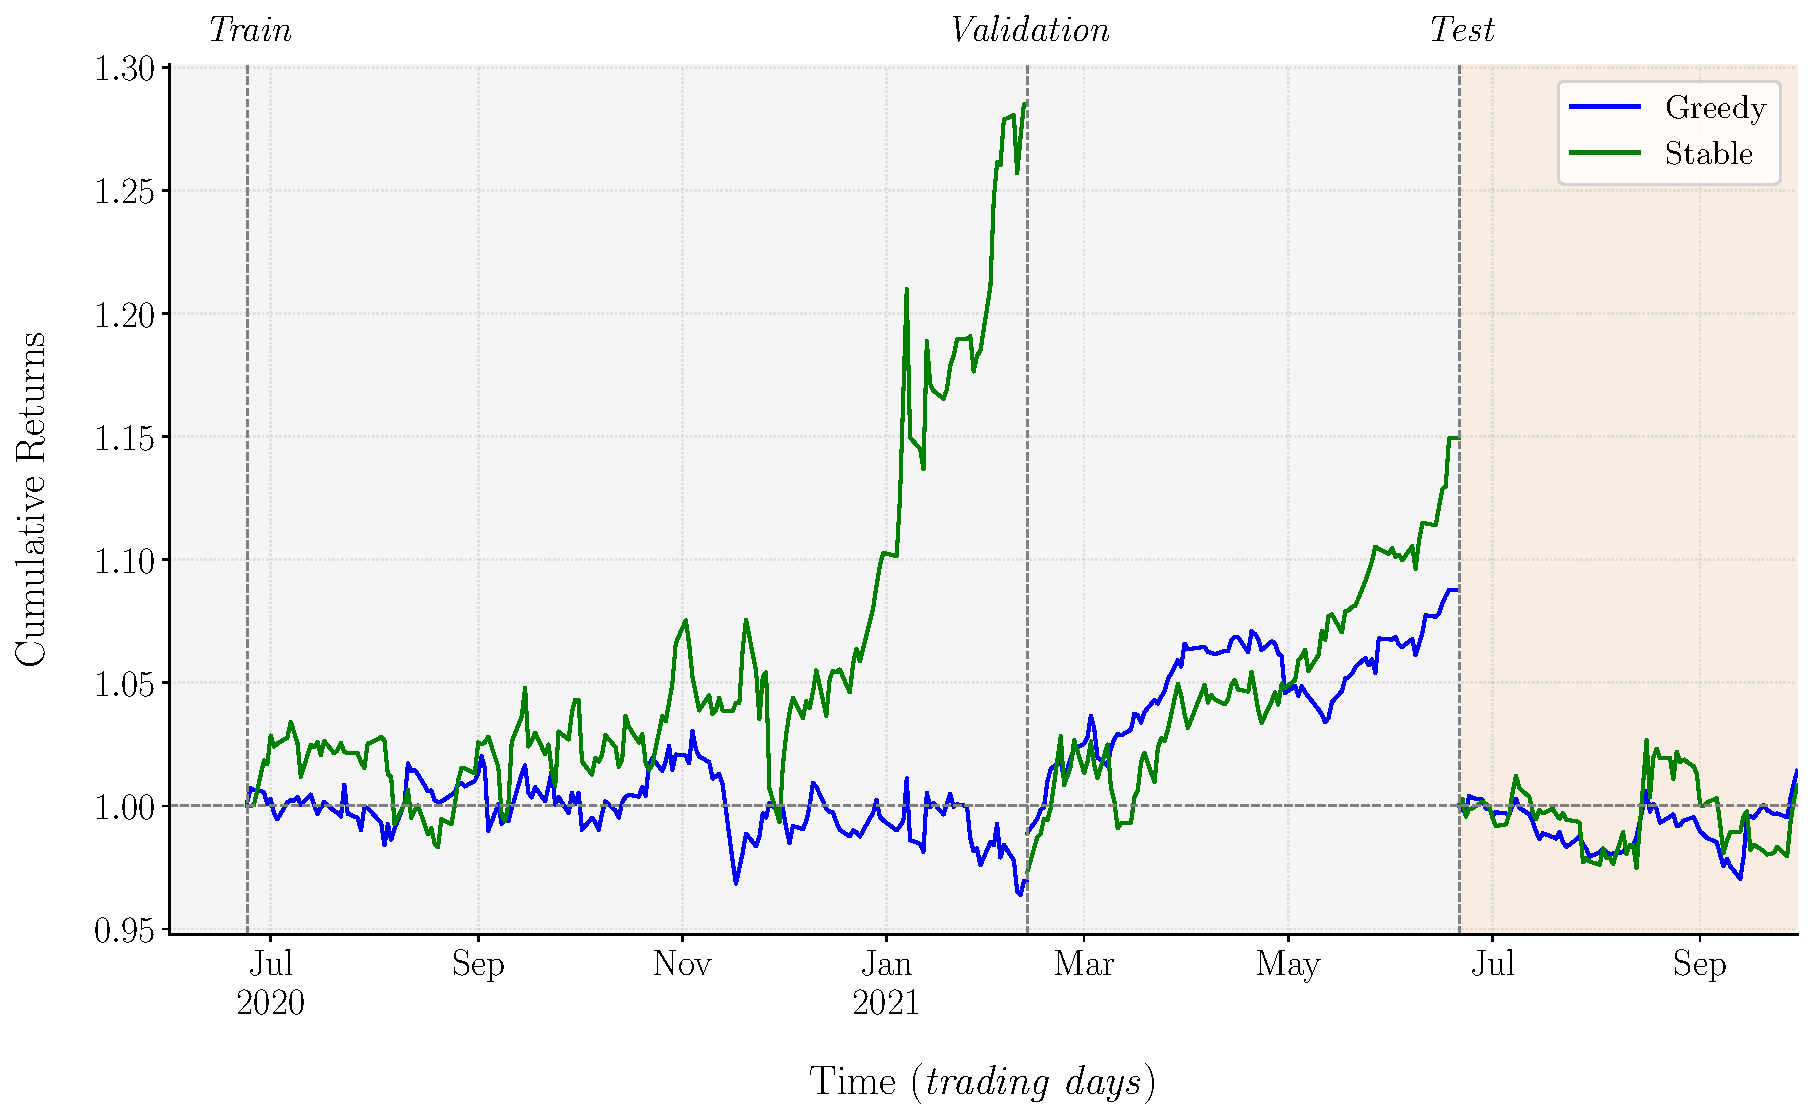
\includegraphics[scale=0.58]{/Users/jesusvillotamiranda/Library/CloudStorage/OneDrive-UniversidaddeLaRioja/CEMFI/Rest/__Second_year__/MasterThesis/__Output/KMeans_Portfolio_Cum_Returns_(L=4,theta=0.5k).pdf}
  \subcaption*{\textit{Note: The holding period of the beta-neutral strategies is set to $L$ = 4 trading days and the number of traded clusters is, $\theta = \integer{0.5k}=13$ as we have $k^*=26$ clusters. The selection criteria for these parameters is based on maximizing the Sharpe Ratios of the train and validation samples.}}
  \label{fig:KMeans_Portfolio_Cum_Returns}
\end{figure}
%----------------------------------------------------


%\red{The correlation between the trading signals generated by the greedy and stable algorithms is 0.512450. What is the correlation in each data split?
%}



%----------------------------------------------------
\inserthere{tab:KMeans_portfolio_statistics}

\begin{table}[H]
    \caption{Statistics of $\mathcal{P}_{\t{KMeans}}$ across data splits}
    \centering
    \renewcommand{\arraystretch}{0.8}
%    \begin{tabular}{|c|c|c|c|c|c|}
    \begin{tabular}{cccccc}
    	\hline \Xhline{2\arrayrulewidth}
%        \rowcolor{gray!10}
        \textbf{Split} & \textbf{Algorithm} & \textbf{Cum. Return} & \textbf{Avg. Return} & \textbf{St. Deviation} & \textbf{Sharpe Ratio} \\
%        \rowcolor{gray!10}
        & & & \textit{(daily)} & \textit{(daily)} & \textit{(annual)} \\
        \hline \Xhline{2\arrayrulewidth}
        \multirow{2}{*}{All}       & \textit{Greedy} & 1.070 & 0.021 & 0.006 & 0.54 \\        & \textit{Stable} & 1.489 & 0.121 & 0.011 & 1.82 \\         \hline          \multirow{2}{*}{Train}       & \textit{Greedy} & 0.969 & -0.019 & 0.007 & -0.41 \\        & \textit{Stable} & 1.285 & 0.151 & 0.012 & 1.97 \\         \hline          \multirow{2}{*}{Validation}       & \textit{Greedy} & 1.088 & 0.094 & 0.005 & 3.23 \\        & \textit{Stable} & 1.149 & 0.155 & 0.008 & 2.93 \\         \hline          \multirow{2}{*}{Test}       & \textit{Greedy} & 1.014 & 0.019 & 0.004 & 0.70 \\        & \textit{Stable} & 1.008 & 0.011 & 0.009 & 0.20 \\         \hline \Xhline{2\arrayrulewidth}
    \end{tabular}
    \label{tab:KMeans_portfolio_statistics}
\vspace{0.5cm}
\subcaption*{\textit{Note: Portfolio statistics of the trading strategy based on clusters obtained from applying KMeans to article embeddings. The statistics provided are: Cumulative Return, Average Return, Standard Deviation and Sharpe Ratio, which have been computed in accordance to the formulas provided in the text. Such statistics are provided for both cluster-selection algorithms: Greedy and Stable. The Greedy algorithm longs (shorts) clusters that maximize (minimize) the cluster-average-$SR$ in the validation sample subject to a positivity (negativity) constraint, while the Stable algorithm longs (shorts) clusters that minimize the rank difference between the training and validation rankings of the cluster-average-$SR$'s subject to a positivity (negativity) constraint, which is now imposed on both sample splits. In both algorithms, the cardinality of each leg is upper-bounded by a hyperparameter $\theta$. 
The holding period of the beta-neutral positions is set to $L$ = 4 trading days and the number of traded clusters is, $\theta = 0.5k=13$ as there are $k^*=26$ KMeans clusters of article embeddings. The selection criteria for these hyperparameters ($L,\theta$) is based on maximizing the Sharpe Ratios of the train and validation samples.
} }
\end{table}
%----------------------------------------------------



%----------------------------------------------------

%----------------------------------------------------
\subsection{LLM-based approach: \qquote{What if an LLM reads the news?}}

\hspace{0.5cm}One may wonder whether empowering an LLM to parse news articles according to a predefined schema that guides it in ellucidating news-implied firm-specific shocks can deliver better insights on how markets react to new information. In this section we will briefly introduce what Large Language Models are, how they have evolved and then, we will dive into how we can guide them to produce an economically structured analysis of business news. 

%%%%%%%%%%%%%%%%%%%%%%%%%%%%%%%%%%%%%%%%%%%%%%%%%%%%%
%%%%%%%%%%%%%%%%%%%%%%%%%%%%%%%%%%%%%%%%%%%%%%%%%%%%%
\subsubsection{Large Language Models}

\hspace{0.5cm}In natural language processing (NLP), Large Language Models (LLMs) are designed to \qquote{understand} and generate human-like text. These models utilize the transformer architecture, which excels in modeling complex language tasks by capturing long-range dependencies and contextual relationships.

\mx 
At the heart of LLMs lies the concept of tokens, which serve as the elemental units of text. Tokens can be individual words, subword units, or characters. Let $x_{1:n}:=\3{x_1, x_2, \ldots, x_n}$ represent a sequence of tokens. The goal of an LLM is to estimate the probability distribution of the next token $x_{n+1}$ conditioned on the previous tokens $x_{1:n}$
$$
\P\2{x_{n+1} \mid \3{x_1, x_2, \ldots, x_n}}
.
$$

%\mx 
An LLM is a neural network architecture designed to learn and approximate this conditional probability distribution over sequences of tokens with a large number of parameters $\Theta$. Namely, we can formulate an LLM as a parameterized function $f_{\Theta}$ that maps a sequence of tokens $\3{x_1, x_2, \ldots, x_n}$ to a probability distribution over the vocabulary, where the parameters $\Theta$ are learned from a large corpus of text training data.
$$
f_{\Theta}:\3{x_1, x_2, \ldots, x_n} \rightarrow 
\P\2{x_{n+1} \mid \3{x_1, x_2, \ldots, x_n} ; \Theta}
$$

%\mx 
Interacting with an LLM involves specifying a prefix sequence $x_{1:n}$, termed the \qquote{prompt}, and sampling the subsequent tokens $x_{n+1:z}$, known as the \qquote{completion}. This process enables users to guide and control the generation of text according to desired contexts and constraints.
$$
\ub{\3{x_1,\ldots,x_n}}{\t{prompt}} \longrightarrow \ub{\3{x_{n+1},\ldots,x_z}}{\t{completion}}
$$


\subsubsection{Evolution of LLMs}
\hspace{0.5cm} The transformer architecture, introduced in the seminal work ``\textit{Attention Is All You Need}'' \citep{vaswani2017attention}, revolutionized LLM development due to its superior handling of long-range dependencies and efficient parallelization of computations.  Subsequent advancements include the encoder-only \texttt{BERT} model \citep{devlin2018bert}, showcasing the power of pre-training on large datasets for fine-tuning on specific tasks. 

\mx 
Conversely, OpenAI's \texttt{GPT} series (\citealp{radford2018improving}) demonstrated the potential of decoder-only models for generative tasks. In particular, the release of \texttt{GPT-3} marked a significant leap in LLM capabilities with its 175 billion parameters and remarkable few-shot learning abilities. This model highlighted the importance of prompt engineering, where carefully crafted prompts can guide model outputs without extensive fine-tuning.  

\mx 
The trend towards open-source models like \texttt{BLOOM} \citep{le2023bloom}, \texttt{Mixtral} and Meta's \texttt{LLaMA} series \citep{touvron2023llama} emphasizes accessibility and transparency in LLM development.  The latest models, including OpenAI's  \texttt{GPT-4o} and \texttt{GPT-o1}, Google's \texttt{Gemini} and \texttt{Mixtral} and \texttt{Gemma}, Anthropic's \texttt{Claude 3.5 Sonnet}, and Meta's \texttt{LLaMA-3}, \texttt{LLaMA-3.1} and  \texttt{LLaMA-3.2} continue to push boundaries with improved accuracy, multimodal capabilities, and larger context windows.

\subsubsection{Function Calling with LlaMA-3}

\hspace{0.5cm} In our endeavor we will employ \texttt{LlaMA-3}, developed by Meta AI and released on April 18, 2024. This model has been pre-trained on approximately 15 trillion tokens of text gathered from ``publicly available sources'' and it comes in two sizes: 8 billion and 70 billion parameters. In this application, we will employ the 70B version, which we will access through an API via \texttt{GroqCloud}.

\mx 
Moreover, we will employ a \textit{function calling} approach to streamline the process of interacting with the LLM. This implies prespecifying a set of functions to the LLM that will then be passed through our dataset of news articles to obtain a structured output in \texttt{JSON} format. The formal procedure is thoroughly described in the Appendix (\cref{alg:function_calling}).

\mx 
Each article $i\in\D$ implies a conversation with the LLM. The structure of the conversation implies defining first a ``system message'', which provides a general context and purpose to the model. In our case:

\begin{quote}
\textit{$-$ You are a function calling LLM that analyses business news in Spanish.  \\
$-$ For every article, you must identify the firms directly affected by the news. Do not include every firm mentioned in the article, only include those that are directly affected by the shocks narrated therein. 
\\
$-$ The identified firms must be Spanish and should be publicly listed in the Spanish exchange (their ticker is of the form `TICKER.MC'). Do not include non-Spanish foreign firms. Do not include Spanish firms that are not publicly traded. \\
$-$ For each identified firm, classify the shocks that affect them (type, magnitude, category). The type of shock can be `demand', `supply', `financial', `policy', or `technology'. The magnitude can be `minor' or `major'. The direction can be `positive' or `negative'. \\
$-$ If a firm is affected neutrally by the news article, don't include it in the analysis.
}
\end{quote}

Then, a news article is fed to the LLM, for example:


%%%%%%%%%%%%%%% ENGLISH VERSION %%%%%%%%%%%%%%%%%%%
\begin{news}
[An article about Cellnex and Telef�nica]
[news:article-cellnex-telefonica]
{Cellnex will face more competition in Europe}
Telef�nica's (TEF.MC) subsidiary, Telxius Telecom, has agreed to sell its telecommunications tower division in Europe and Latin America to American Tower (AMT), which will expand the latter's presence in Europe and increase competition for the Spanish wireless telecommunications group Cellnex Telecom (CLNX.MC), according to Equita Sim. The transaction "represents the entry of a new independent tower operator into the Spanish market and potentially more competition for future growth in the European market as well," says the brokerage firm.		
\end{news}

Next, we define an umbrella function \qquote{firms}, which asks the LLM to identify the set $\F^i_{LLM}$ for each $i\in\D$. Then, for each $j\in\F_{LLM}^i$ we ask the LLM to categorize the type, expected magnitude, and expected direction that the shock described in the article implies in that particular firm $j$.
%----------------------------------------------------
\inserthere{tab:function_calling_structure}

\begin{table}[H]
\centering
\begin{threeparttable}
\caption{Function calling schema}
%{\footnotesize
%\renewcommand{\arraystretch}{1}
\begin{tabular}{lL{4.1cm}L{6.8cm}L{5cm}}
%%%%%%%%%%%%%%%%%%%%%%%%%%%%%%%%%%%%%%%%%%%%%%%%%%%%%
%%%%%%%%%%%%%%%%%%%%%%%%%%%%%%%%%%%%%%%%%%%%%%%%%%%%%
\hline \Xhline{2\arrayrulewidth}
%\rowcolor{gray!10}
\multicolumn{2}{l}{\textbf{Function}} & \textbf{Prompt} & \textbf{Options} \tabularnewline
\hline \Xhline{2\arrayrulewidth} 
\multicolumn{2}{l}{1. \texttt{firms}} & \qquote{List all the firms affected by the events narrated in the article} & \texttt{array} \tabularnewline
\hline
 & 1.1. \texttt{firm} & \qquote{Iterate over each \textnormal{\texttt{firm}} in \textnormal{\texttt{firms}}} & \texttt{string}
 \tabularnewline
\cline{2-4} \cline{3-4} \cline{4-4} 
 & 1.2. \texttt{ticker} & \qquote{State the stock market ticker of \textnormal{\texttt{firm}} } & \texttt{string}
 \tabularnewline
\cline{2-4} \cline{3-4} \cline{4-4} 
 & 1.3. \texttt{shock\_type} & \qquote{What type of shock does this article imply on \textnormal{\texttt{firm}} ?} & \{demand, supply, financial, \newline technology, policy\}\tabularnewline
\cline{2-4} \cline{3-4} \cline{4-4} 
 & 1.4. \texttt{shock\_magnitude} & \qquote{How much impact is this shock expected to have on \textnormal{\texttt{firm}}?} & \{minor, major\}\tabularnewline
\cline{2-4} \cline{3-4} \cline{4-4} 
 & 1.5. \texttt{shock\_direction} & \qquote{In what direction is this shock expected to impact \textnormal{\texttt{firm}}?} & \{positive, negative\}\tabularnewline 
%\cline{2-4} \cline{3-4} \cline{4-4} 
\hline \Xhline{2\arrayrulewidth}
\end{tabular}
%}
\begin{tablenotes}
\footnotesize
\mx
\item \textit{Note: 
For clarity of exposition, the actual prompts passed to LlaMA are avoided here but can be found in the code. 
%The ``Options'' column imposes the asnwer format that the LLM must follow. For example, in \texttt{firms}, the option \texttt{array} indicates that the answer must be an enumeration of firms, while the option \texttt{string} in the subfunctions \texttt{firm} and \texttt{ticker} indicates that the answer must be a single name. Finally, the \texttt{shock\_} subfunctions ask the LLM to choose from a predefined set of options.
}
\end{tablenotes}
\label{tab:function_calling_structure}
\end{threeparttable}
\end{table}



%%%%%%%%%%%%%%%%%%%%%%%%%%%%%%%%%%%%%%%%%%%%%%%%%%%%%
%%%%%%%%%%%%%%%%%%%%%%%%%%%%%%%%%%%%%%%%%%%%%%%%%%%%%

%\begin{table}[H]
%\centering
%\begin{threeparttable}
%\caption{Function calling schema}
%{\small
%\begin{tabular}{l||L{4.1cm}|L{6.8cm}|L{5cm}|}
%%%%%%%%%%%%%%%%%%%%%%%%%%%%%%%%%%%%%%%%%%%%%%%%%%%%%%
%%%%%%%%%%%%%%%%%%%%%%%%%%%%%%%%%%%%%%%%%%%%%%%%%%%%%%
%\hline 
%\multicolumn{2}{|l|}{Function} & Description & Options \tabularnewline
%\hline 
%\hline 
%%\multicolumn{2}{|l|}{1. \texttt{publication\_time}} & Date and time of publication & ``''\tabularnewline
%%\hline 
%%\multicolumn{2}{|l|}{2. \texttt{scope}} & Scope or focus of the news article's impact. & \{Firm, Industry, Economy\}\tabularnewline
%%\hline 
%%\multicolumn{2}{|l|}{3. \texttt{news\_category}} & Type of information provided in the article & \{New, Historical, \newline Analysis/Comments\}\tabularnewline
%%\hline 
%\multicolumn{2}{|l|}{1. \texttt{firms}} & List all the firms affected by the events narrated in the article & \texttt{array} \tabularnewline
%\hline
% & 1.1. \texttt{firm} & Iterate over each firm in \texttt{firms} & \texttt{string}
% \tabularnewline
%\cline{2-4} \cline{3-4} \cline{4-4} 
% & 1.2. \texttt{ticker} & State the stock market ticker of this firm & \texttt{string}
% \tabularnewline
%\cline{2-4} \cline{3-4} \cline{4-4} 
% & 1.3. \texttt{shock\_type} & What type of shock does the article imply on this firm? & \{demand, supply, financial, \newline technology, policy\}\tabularnewline
%\cline{2-4} \cline{3-4} \cline{4-4} 
%% & 4.4. \texttt{shock\_duration} & Expected duration of the shock on this firm & \{Short term, Mid term, Long term\}\tabularnewline
%\cline{2-4} \cline{3-4} \cline{4-4} 
% & 4.5. \texttt{shock\_magnitude} & How much imapct is the shock expected to have on this firm? & \{minor, major\}\tabularnewline
%\cline{2-4} \cline{3-4} \cline{4-4} 
% & 4.6. \texttt{shock\_direction} & In what direction is the shock expected to impact this firm? & \{positive, negative\}\tabularnewline 
%\cline{2-4} \cline{3-4} \cline{4-4} 
%% & 4.6. \texttt{trading\_signal} & Trading decision on this firm's stock & \{Long, Not trade, Short\}\tabularnewline
%%\cline{2-4} \cline{3-4} \cline{4-4} 
%% & 4.7. \texttt{market\_timing} & Time of incorporation of the shock on this firm's stock price (\textit{today=publication date}). & \{Before last week, Last week, \newline Yesterday, Today, Tomorrow, \newline Next week, After next week\}\tabularnewline
%%\cline{2-4} \cline{3-4} \cline{4-4} 
%%%%%%%%%%%%%%%%%%%%%%%%%%%%%%%%%%%%%%%%%%%%%%%%%%%%%%
%%%%%%%%%%%%%%%%%%%%%%%%%%%%%%%%%%%%%%%%%%%%%%%%%%%%%%
%\end{tabular}
%}
%\begin{tablenotes}
%\footnotesize
%\mx
%%\item \textit{Note}: A justification of the category choice is asked for all the parameters with an asterisk . 
%\item \textit{Note: For clarity of exposition, the actual prompts passed to Llama are avoided here but can be found in the Appendix. The ``Options'' column imposes the asnwer format that the LLM must follow. For example, in \texttt{firms}, the option \texttt{array} indicates that the answer must be an enumeration of firms}, while the option \texttt{string} in the subfunctions \texttt{firm} and \texttt{ticker} indicates that the answer must be a single name. Finally, the shock subfunctions ask the LLM to choose an option from a predefined set of options.
%\end{tablenotes}
%\end{threeparttable}
%\end{table}
%----------------------------------------------------

The function calling schema is outlined in \cref{tab:function_calling_structure}. First, we need to prompt the LLM, and then we need to specify the desired format of its response. The ``Options'' column imposes the answer format that the LLM must follow. For example, in \texttt{firms}, the ``\texttt{array}'' option indicates that the answer must be an enumeration of firms, while the  ``\texttt{string}'' option in the subfunctions \texttt{firm} and \texttt{ticker} indicates that the answer must be a single name. Finally, the \texttt{shock\_} subfunctions ask the LLM to choose from a predefined set of possible responses.

\mx 
Note that the firms identified by the LLM are used to validate the firms identified by the pattern recognition algorithm (those extracted with \texttt{regex} by exploiting the pattern \texttt{<WORD>.MC}). As mentioned earlier, given the high quality of the filtered dataset (the ticker of the firms that are actively involved in the article are explicitly stated), they are almost identical. Hence, we indistinctively use $\F_i$ to simplify notation.

\mx 
The output provided by the LLM comprises two parts: a \qquote{Structured output}, and an \qquote{Unstructured output} justifying the choices made in the \qquote{Structured output}. The unstructured part is employed to validate the LLM's output. 
 By manually reading a small random subsample of such unstructured outputs from the LLM, we can quickly determine whether the LLM has correctly understood the task. If the LLM exhibits confusion, hallucination patterns become apparent in the unstructured output, indicating the need to refine the system instructions and tool descriptions within the function-calling schema to clarify the task for the LLM.

\begin{quote}

\textbf{1) Structured Output: } 

\vspace{0.2cm}
	\begin{tabular}{ccccc}
		\hline \Xhline{2\arrayrulewidth}
		\texttt{firm} & \texttt{ticker} & \texttt{shock\_type} & \texttt{shock\_magnitude} & \texttt{shock\_direction}
		\\ \hline \Xhline{2\arrayrulewidth} 
		Cellnex Telecom & CLNX.MC & supply & minor & negative
		\\ 
		Telef�nica & TEF.MC & financial & minor & positive
		\\ 
		\hline \Xhline{2\arrayrulewidth}
	\end{tabular}
\vspace{0.2cm}

\textbf{2) Unstructured Output (justification)}

\textit{The news about American Tower's expansion in Europe may increase competition for Cellnex, which is why it's classified as a negative supply shock. On the other hand, Telef�nica benefits from the sale of its tower division, which is why it's classified as a positive financial shock.}

\end{quote}

This procedure is run iteratively from beginning (defining system prompt) to end (getting the output) for every $i\in\D$.\footnote{
This procedure was run on a MacBook Pro M2 with 16GB RAM, 12-core central processing units (CPU), 19-core graphics processing units (GPU), and 16-core Neural Engine. The first run of the code takes about 18.4 hours; however, successive runs were required afterwards with smaller subsets of failed articles, as the LLM always raises errors for a certain percentage of the articles that are fed to it.
}

%%%%%%%%%%%%%%%%%%%%%%%%%%%%%%%%%%%%%%%%%%%%%%%%%%%%%
%%%%%%%%%%%%%%%%%%%%%%%%%%%%%%%%%%%%%%%%%%%%%%%%%%%%%

\subsubsection{Clustering with the LLM}
Formally, we can define the set $\mathcal B:=\{(i,j)\mid i\in \D ~\wedge~j\in\mathcal F^i \}$ containing all the unique pairs of articles and identified firms. 
The LLM assigns each pair $(i,j)\in \mathcal B$ with a choice from each of the following sets:
$$
\begin{array}{llll}
\t{\qquote{shock type}}
&& \mathcal{S}_T
& := \{\t{demand, supply, financial, technology, policy}\}
\\[0.3em]
\t{\qquote{shock magnitude}}
&& \mathcal{S}_M
& :=\{\t{minor, major}\} 
\\[0.3em]
\t{\qquote{shock direction}}
&& \mathcal{S}_D
& := \{\t{positive, negative}\}
\end{array}
$$
The clustering of news articles follows naturally by taking the Cartesian product of these three sets:
$
\mathcal{G}_{LLM} := \mathcal{S}_T \times \mathcal{S}_M \times \mathcal{S}_D
,
$
and the total number of clusters is now $k_{LLM} =|\mathcal{G}_{LLM}|=20$. 
Consequently, a news article to which the LLM assigns $s_T\in\mathcal{S}_T$, $s_M\in\mathcal{S}_M$, $s_D\in\mathcal{S}_D$ will belong to cluster $(s_T,s_M, s_D)\in \mathcal{G}_{LLM}$. Formally, the set of all possible clusters is defined as: 
$$
\mathcal{G}_{LLM} := \3{(s_T,s_M, s_D) \c  s_T\in\mathcal{S}_T, s_M\in\mathcal{S}_M, s_D\in\mathcal{S}_D}
,
$$
and each cluster can then be mapped to a positive integer as $\mathcal G_{LLM}\to \{k\in \mathbb{N}_0 \mid 0\leq k\leq 19\}$.
A representative sample of 3 articles from each cluster is provided in the Appendix \cref{tab:LLM_Articles_3_English}. 

%%%%%%%%%%%%%%%%%%%%%%%%%%%%%%%%%%%%%%%%%%%%%%%%%%%%%
\mx 
In \cref{fig:LLM_cluster_distribution} we plot the distribution of news articles through clusters. As we can see, most articles are assigned to clusters 8, 9, 10, and 11, which are the clusters referred to financial events or shocks. Such clusters are mostly composed of articles about the publication of quarterly and semiannual results. More specifically, cluster 8 (\textit{financial, minor, positive}) concentrates around 1/3 of the sample and is associated to the publication of results that mildly surpass the expectations of investors, hence, making this cluster a good candidate for a long trading signal.

\mx 
On the other hand, other clusters such as 16 (\textit{policy, minor, positive}) and 0 (\textit{demand, minor, positive}) also concentrate a big share of news. Note that no cluster has been assigned to cluster 13 (\textit{technology, minor, negative}).
%
Different from KMeans clustering with embeddings, now the distribution profile of articles through clusters becomes very stable across data splits. This shows that clustering based on a comprehensive analysis of the shocks implied by the article on the affected firms is really stable over time, which constitutes a promising result.

%----------------------------------------------------
%----------------------------------------------------
\inserthere{fig:LLM_cluster_distribution}
\begin{figure}[H]
    \centering
    \caption{Distribution of articles through LLM clusters}
    
    % Upper plot
    \begin{subfigure}[b]{\textwidth}
        \caption{All data ($\mathcal D$)}
        \centering
        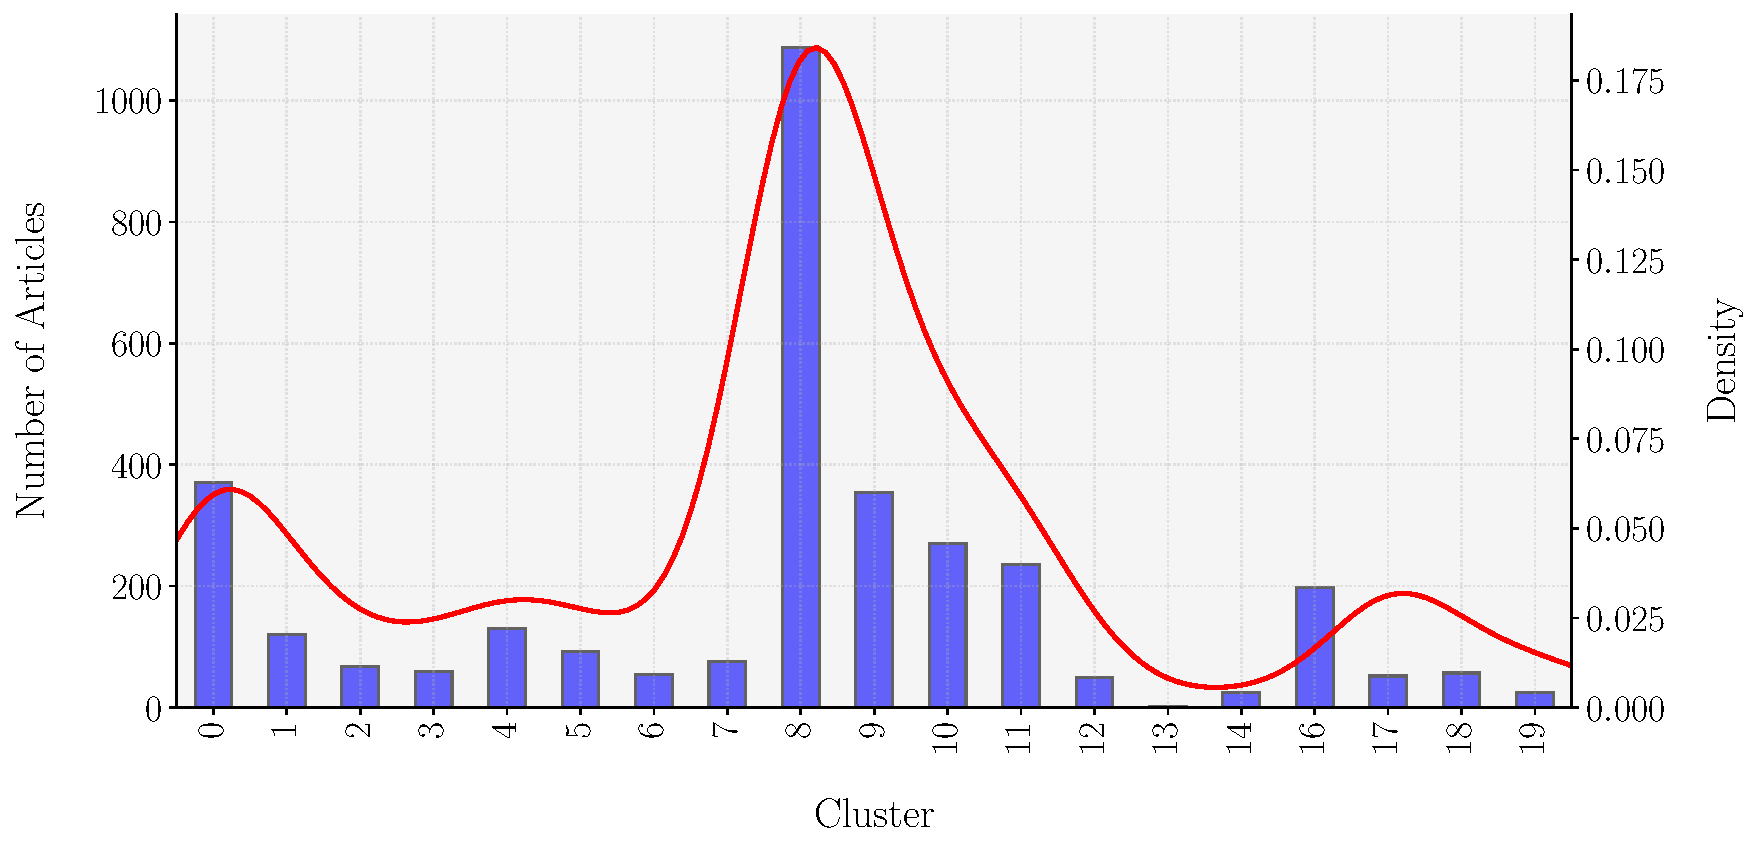
\includegraphics[scale=0.48]{fig_LLAMA_Cluster_Distribution.pdf}
        \label{fig:all_data}
    \end{subfigure}

    % Lower plots
    \begin{subfigure}[b]{0.32\textwidth}
        \caption{Training data ($\D^{tr}$)}
        \centering
        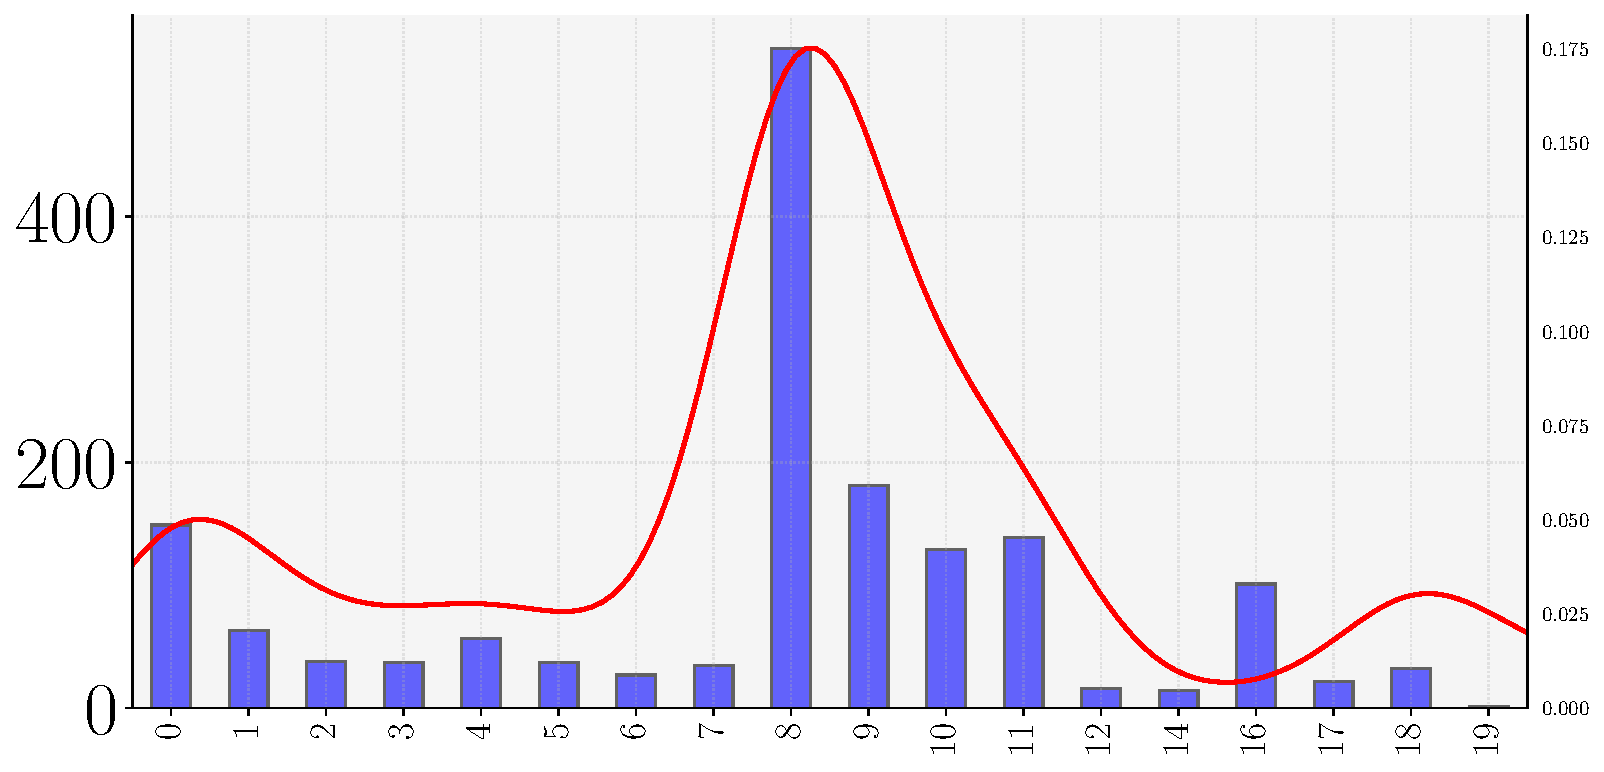
\includegraphics[width=\textwidth]{fig_LLAMA_Cluster_Distribution_Train.pdf}
        \label{fig:train_data}
    \end{subfigure}
    \begin{subfigure}[b]{0.32\textwidth}
        \caption{Validation data ($\D^{val}$)}
        \centering
        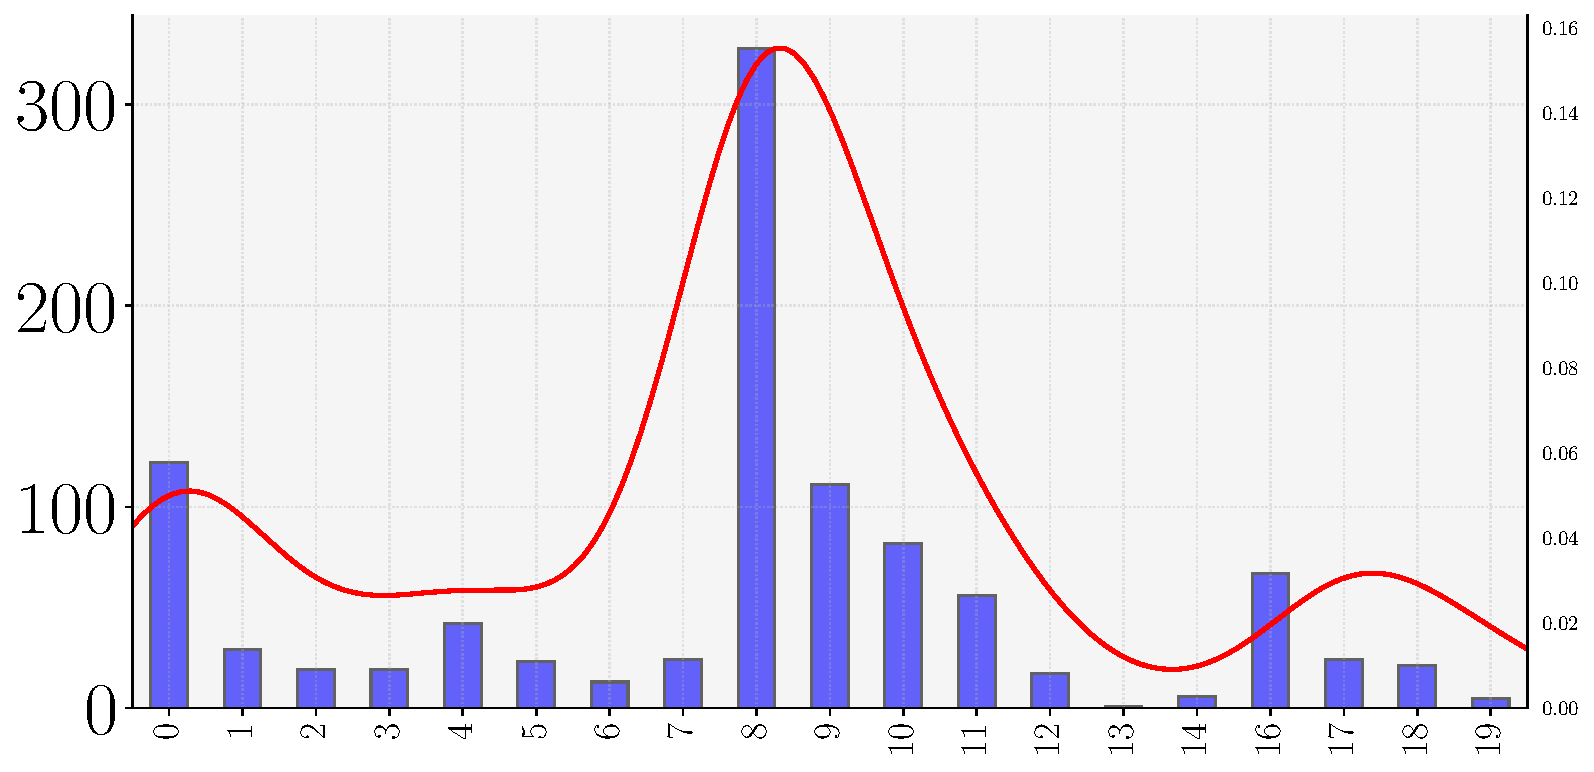
\includegraphics[width=\textwidth]{fig_LLAMA_Cluster_Distribution_Validation.pdf}
        \label{fig:val_data}
    \end{subfigure}
    \begin{subfigure}[b]{0.32\textwidth}
        \caption{Test data ($\D^{test}$)}
        \centering
        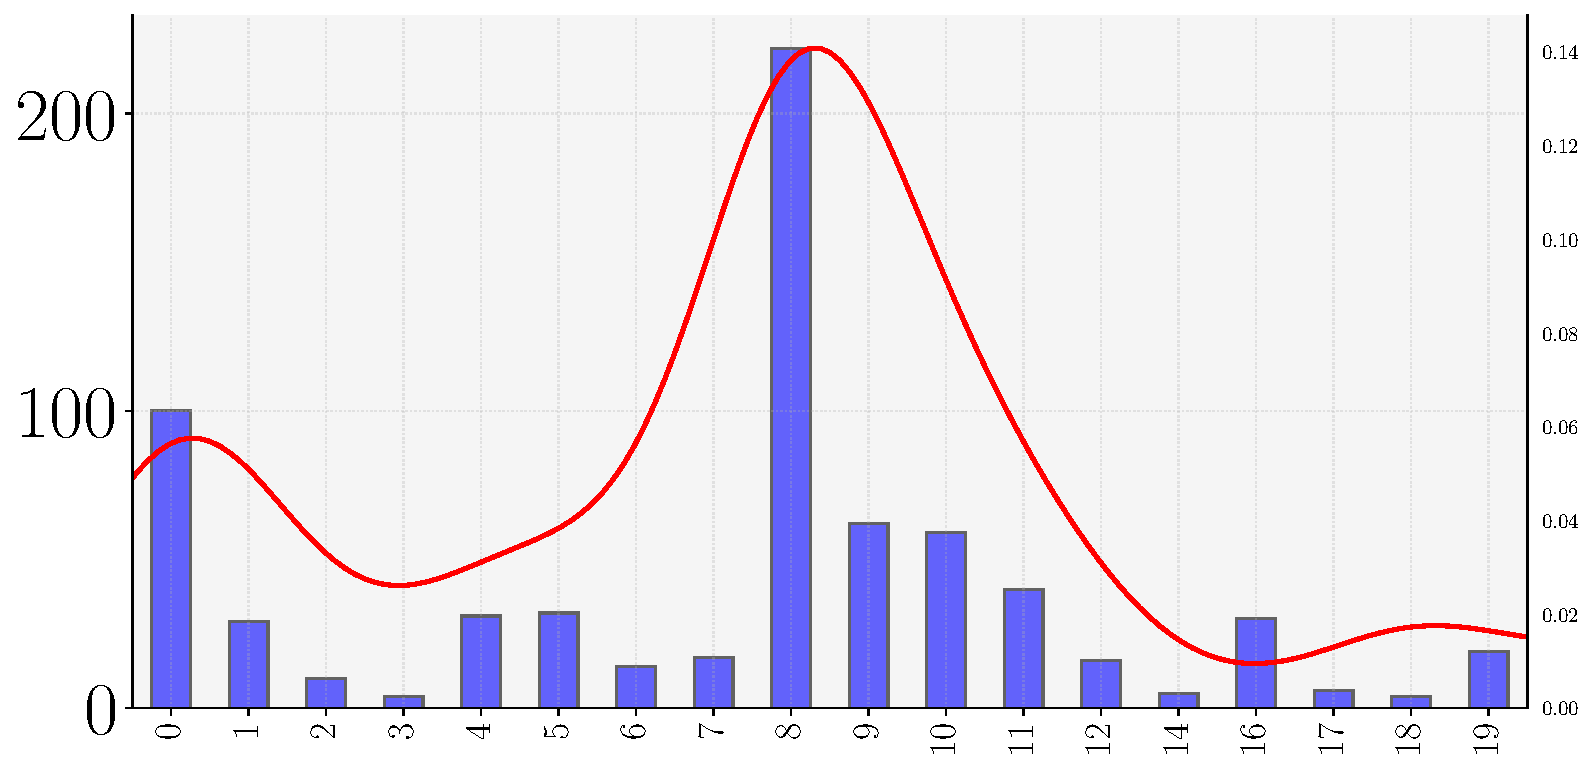
\includegraphics[width=\textwidth]{fig_LLAMA_Cluster_Distribution_Test.pdf}
        \label{fig:test_data}
    \end{subfigure}
    \label{fig:LLM_cluster_distribution}
    \subcaption*{\textit{Note: This figure presents the distribution of news articles across clusters derived using an LLM-based approach. The upper plot shows the distribution for the entire dataset ($\mathcal D$), while the lower plots display the distributions for the training ($\D^{tr}$), validation ($\D^{val}$), and test ($\D^{test}$) datasets. Clusters 8, 9, 10, and 11, which capture financial events or shocks, dominate the distribution, with cluster 8 (\textit{financial, minor, positive}) representing approximately one-third of the dataset. This cluster includes articles related to financial reports with mildly positive outcomes, potentially offering insight for long trading signals. Unlike KMeans clustering with embeddings, this LLM-based clustering shows stable distributions across data splits, highlighting the robustness of this method over time. }}
\end{figure}
%----------------------------------------------------
%----------------------------------------------------


%----------------------------------------------------




\section{Trading Strategy}

%----------------------------------------------------
\subsection{Beta-neutral positions on every $(i,j)\in\mathcal B$}
Since we are interested in the individual effect of an article $i\in\D$ in each of the affected firms $j\in\F^i$, we work with the set
$
\mathcal{B}:=\3{(i,j) \mid i\in \D ~\wedge~j\in \F^i }
$, where $\abs{\mathcal{B}}=3410>\abs{\D}=2613$. 
We then fit a market model to each unique pair $(i,j)\in \mathcal{B}$
on some window of time $\mathcal{M}^i\subset \tilde{\mathfrak{d}}$ before the effective treatment day: 
\footnote{To rigorously define $\mathcal M^i$, we need to work with the index and inverse index functions. 
\begin{itemize}
  \item \textbf{Index Function}. 
Given a finite ordered set $\mathcal{Z}=\left\{z_1, z_2, \ldots, z_n\right\}$, the index function 
$\mathbb{I}_{\mathcal{Z}}: \mathcal{Z} \rightarrow\{1,2, \ldots,|\mathcal{Z}|\}$
 maps an element $z\in\Z$ to its position in the ordered set $\mathcal{Z}$. Formally:
$
\mathbb{I}_{\mathcal{Z}}(z_{\ell})=\ell 
~ \text { for } ~ \ell \in\{1,2, \ldots,|\mathcal{Z}|\}
.
$

\item \textbf{Inverse Index Function}. 
The inverse index function 
$\mathbb{I}_{\mathcal{Z}}^{-1}:\{1,2, \ldots,|\mathcal{Z}|\} \rightarrow \mathcal{Z}$
 retrieves the element $z \in \mathcal{Z}$ corresponding to a given index ${\ell}$.
Formally:
$
\mathbb{I}_{\mathcal{Z}}^{-1}({\ell})=z_{\ell} ~\text { for } ~{\ell} \in\{1,2, \ldots,|\mathcal{Z}|\}
.$
\end{itemize}
For the market model window, we use $\mathbb{I}_{\tilde{\mathfrak{d}}}$ and $\mathbb{I}^{-1}_{\tilde{\mathfrak{d}}} $ applied to the set of trading days $\tilde{\mathfrak d}$. Namely:
$$
\mathcal{M}^i := 
\3{
d\in \tilde{\mathfrak{d}}
\c 
\mathbb{I}^{-1}_{\tilde{\mathfrak{d}}} 
\1{
\mathbb{I}_{\tilde{\mathfrak{d}}} (\tilde{d}_0^i) - {w}_b - {w}_m 
}
\leq d \leq 
\mathbb{I}^{-1}_{\tilde{\mathfrak{d}}} 
\1{ 
\mathbb{I}_{\tilde{\mathfrak{d}}} (\tilde{d}_0^i) - {w}_b 
}
}
,
$$
with a buffer of ${w}_b=10$ trading days before the effective treatment date, and a market model window length of ${w}_m=100$ trading days.



}
%----------------------------------------------------
$$
r_{d}^{j} = \alpha^{(i,j)} + \beta^{(i,j)} r_{d}^M + \epsilon_{ d}^{(i,j)} 
\qquad  
\forall d \in \mathcal{M}^i
,
$$
where 
$r_{d}^{j}$ denotes the return of firm $j$ at trading day $d$ in excess of the risk-free asset, which we take to be the daily euro short-term rate (\texttt{\euro STR}),
and 
$r_{d}^M$ denotes the excess return of the market (IBEX-35).  
%----------------------------------------------------
These returns are obtained from the adjusted close price, which corrects the price evolution for corporate actions such as dividends, stock splits, and new stock issuance.\footnote{
The adjusted close price ensures that the returns reflect the true economic gains or losses for an investor holding the stock. 
%
Formally, the return of firm $j$ between two trading days $d_1, d_2\in \tilde{\mathfrak{d}}$ is computed as:
$
r_{d_1:d_2}^{j} = 
(
p_{d_2}^{j,\text{adj}} - p_{d_1}^{j,\text{adj}}
)/(
p_{d_1}^{j,\text{adj}}
)
$
where $p_{d}^{j,\text{adj}}$ is the adjusted close price of firm $j$ at trading day $d$.
}
%----------------------------------------------------

\mx 
%----------------------------------------------------
The notation overload in the regression coefficients $(\alpha^{(i,j)},\beta^{(i,j)})$ emphasizes the fact that $\alpha$ and $\beta$ are specific to each pair $(i,j)\in\mathcal B$ since the market model is computed for each firm $j\in\F_{\t{IBEX-35}}$ on some specific window of time $\mathcal{M}^i$, which is particular to each article $i\in\D$.
%----------------------------------------------------

\mx 
The reason why we fit a market model to each $(i,j)\in\mathcal B$ is to then apply a market-neutral strategy as in \cite{chan2003stock} and \cite{jiang2021pervasive}. This is an investment approach designed to minimize or eliminate exposure to overall market movements, isolating the performance of a specific firm. 
% 
In particular, we employ a beta-neutral strategy by buying one unit of firm $j$'s stock and shorting $\beta^{(i,j)}$ units of the market index (i.e.: an ETF replicating the IBEX-35). 

%----------------------------------------------------
\mx
This hedged position harvests the idiosyncratic returns from the market model and it only makes sense when firm $j$'s returns are expected to outperform or underperform the market.\footnote{
For expected underperformance of firm $j$, reverse the beta neutral positions: 
sell one unit of firm $j$ and buy $\beta^{(i,j)}$ units of the market index. However, note that this will be handled later by a Trading Rule $(TR)$.
\mx 
}
The position delivers abnormal returns $AR^{(i,j)}_{d}$ at some trading day $d\geq \tilde{d}_0^i$ given by
\begin{align*}
r_{d}^j -  \beta^{(i,j)} r_{d}^M = \alpha^{(i,j)} + \epsilon_{d}^{(i,j)} =: AR^{(i,j)}_{d}
.
\end{align*}
%----------------------------------------------------
The position is taken at the effective treatment date $\tilde d_0^i$ and is maintained over a holding window $\mathcal H^i \subset \tilde{\mathfrak{d}}$ consisting of $L\in\mathbb{N}$ trading days after $\tilde d_0^i$, where $L$ is set to 4 trading days.\footnote{  
The holding period of the position is defined as 
$
\mathcal H^i:=
\3{
d \in \tilde{\mathfrak{d}}
\c 
\tilde{d}_0^i
\leq d \leq 
\mathbb{I}^{-1}_{\tilde{\mathfrak{d}}}\1{\mathbb{I}_{\tilde{\mathfrak{d}}}(\tilde d_0^i)+L}}
$}
%----------------------------------------------------
The justification for this choice of $L$ is made in section A.2 of the Appendix. 

%----------------------------------------------------
\mx 

After having held the beta-neutral position over the holding period $\mathcal H^i$, we obtain a time series of abnormal returns $\{AR_{d}^{(i,j)}\}_{d\in\mathcal H^i}$ from where we can obtain the usual performance metrics. First, the average daily log returns are obtained as
$$
\mu^{(i,j)} = \frac{1}{{{L}}+1} 
\sum_{d\in \mathcal H^i}
\ln\4{1+AR_d^{(i,j)}}
~,
$$
Then, the standard deviation is given by
$$
\sigma^{(i,j)}
=
\sqrt{
\frac{1}{{{L}}}
\sum_{d\in \mathcal H^i}
[
\ln(1+AR_d^{(i,j)}) - \mu^{(i,j)}
]
^2}
~.
$$

\mx 
And finally, the annualized Sharpe Ratio can be obtained by scaling the daily Sharpe Ratio by the square root of ${252}$, which are the typical number of trading days in a year according to the Spanish calendar. 
$$
SR^{(i,j)} =
\sqrt{252}~
\frac{
\mu^{(i,j)}
}{
\sigma^{(i,j)}
}
~.
$$
%%%%%%%%%%%%%%%%%%%%%%%%%%%%%%%%%%%%%%%%%%%%%%%%%%%%%
\subsection{Optimal Cluster Selection}
%%%%%%%%%%%%%%%%%%%%%%%%%%%%%%%%%%%%%%%%%%%%%%%%%%%%%

After taking beta-neutral positions on each pair $(i,j)\in\mathcal B$ and holding them over some window $\mathcal H^i$, we can obtain a measure of how profitable the positions are on average for articles that belong to the same cluster $g\in\mathcal G$. For this purpose, let $\mathcal{B}_g$ denote the set of all article and firm pairs such that the article belongs to some cluster $g\in\mathcal G$. 
$$
\mathcal{B}_g:= \{(i,j) \mid (i,j)\in\mathcal{B} ~\wedge~ i \in \D_g \}
.
$$
The average Sharpe Ratio associated to each cluster is
$$
\overline{S R}_g=\frac{1}{\left|\mathcal{B}_g\right|} \sum_{(i,j) \in \mathcal{B}_g} S R^{(i,j)}
,
$$
and it provides a measure of the performance of the beta-neutral positions in each cluster. 

%%%%%%%%%%%%%%%%%%%%%%%%%%%%%%%%%%%%%%%%%%%%%%%%%%%%%
%%%%%%%%%%%%%%%%%%   KMEANS   %%%%%%%%%%%%%%%%%%%%%%%
%%%%%%%%%%%%%%%%%%%%%%%%%%%%%%%%%%%%%%%%%%%%%%%%%%%%%

In the case of KMeans, the distribution of cluster-average Sharpe Ratios across the different clusters is plotted in \cref{fig:KMeans_distr_avg_SR}. In the validation set, they are centered at 0, but we observe some outliers with unusually low and high average $SR$. On the other hand, the distributions in the train and test data are slightly skewed to the right and show no presence of substantial outliers.

%----------------------------------------------------
\inserthere{fig:KMeans_distr_avg_SR}
\begin{figure}[H]
  \centering
  \caption{Distribution of Embeddings-based Cluster-Average Sharpe Ratios $(\overline{SR}_g)$ by Split}
  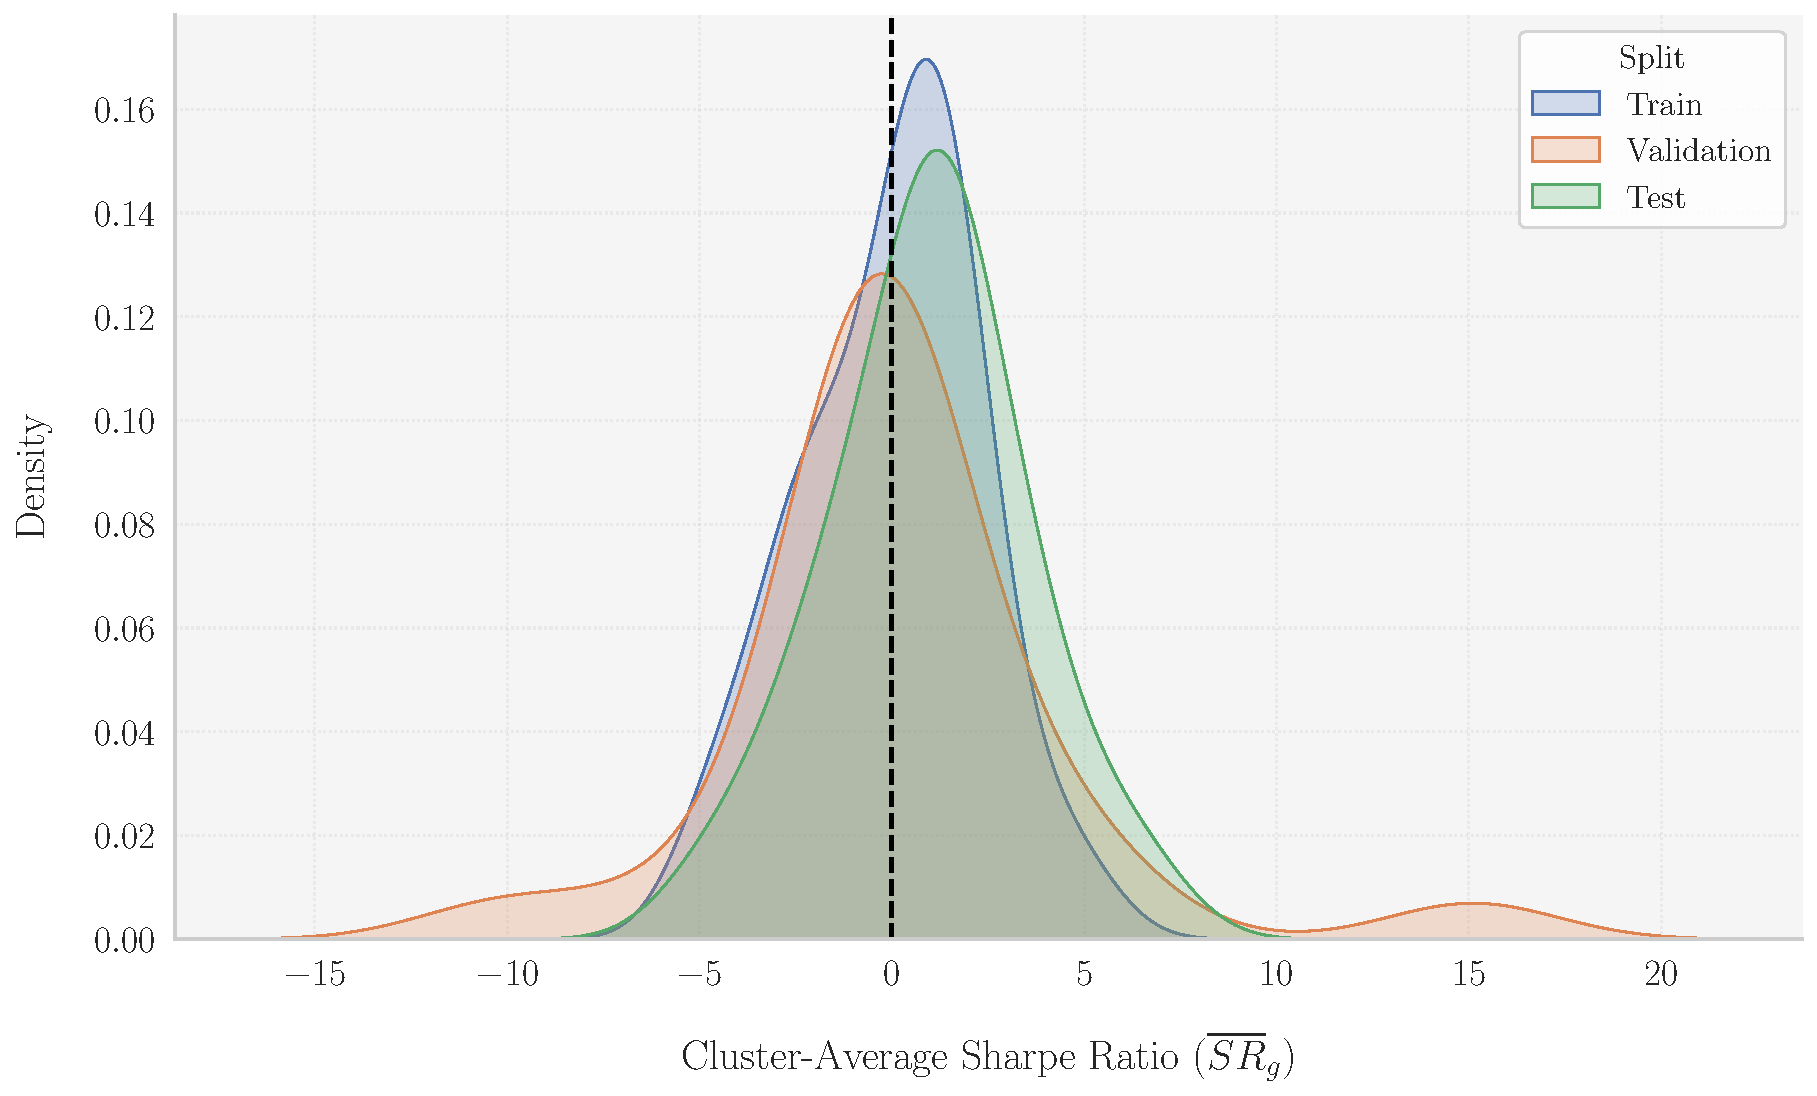
\includegraphics[scale=0.45]{fig_KMeans_Cluster-Avg_SR_Distribution.pdf}
\label{fig:KMeans_distr_avg_SR}
\subcaption*{\textit{Note: This figure shows the distribution of cluster-average Sharpe Ratios $(\overline{SR}_g)$ for the embeddings-based KMeans clusters across the different data splits: training, validation, and test sets. Each Sharpe Ratio is computed as the average of beta-neutral positions associated with articles in a given cluster. In the validation set, the distribution is centered around 0, with a few outliers showing unusually high or low Sharpe Ratios. Conversely, the distributions in the training and test sets are slightly skewed to the right, suggesting better performance in certain clusters, with no significant presence of outliers.}}

\end{figure}
%----------------------------------------------------

%%%%%%%%%%%%%%%%%%%%%%%%%%%%%%%%%%%%%%%%%%%%%%%%%%%%%
%%%%%%%%%%%%%%%%%%%%   LLM   %%%%%%%%%%%%%%%%%%%%%%%%
%%%%%%%%%%%%%%%%%%%%%%%%%%%%%%%%%%%%%%%%%%%%%%%%%%%%%
In the case of LLM-based clustering, all distributions are left-skewed. The distribution in the training sample has fat tails which severely contrasts with the light-tailed distribution of the validation sample. In the test data, we observe a bell-shaped distribution with some accumulation of mass at high $SR$s (between 5 and 15), indicating stronger performance in some clusters.
%----------------------------------------------------
\inserthere{fig:LLM_cluster-average-SR-by-split}
\begin{figure}[H]
  \centering
  \caption{Distribution of LLM-based Cluster-Average Sharpe Ratios $(\overline{SR}_g)$ by Split}
  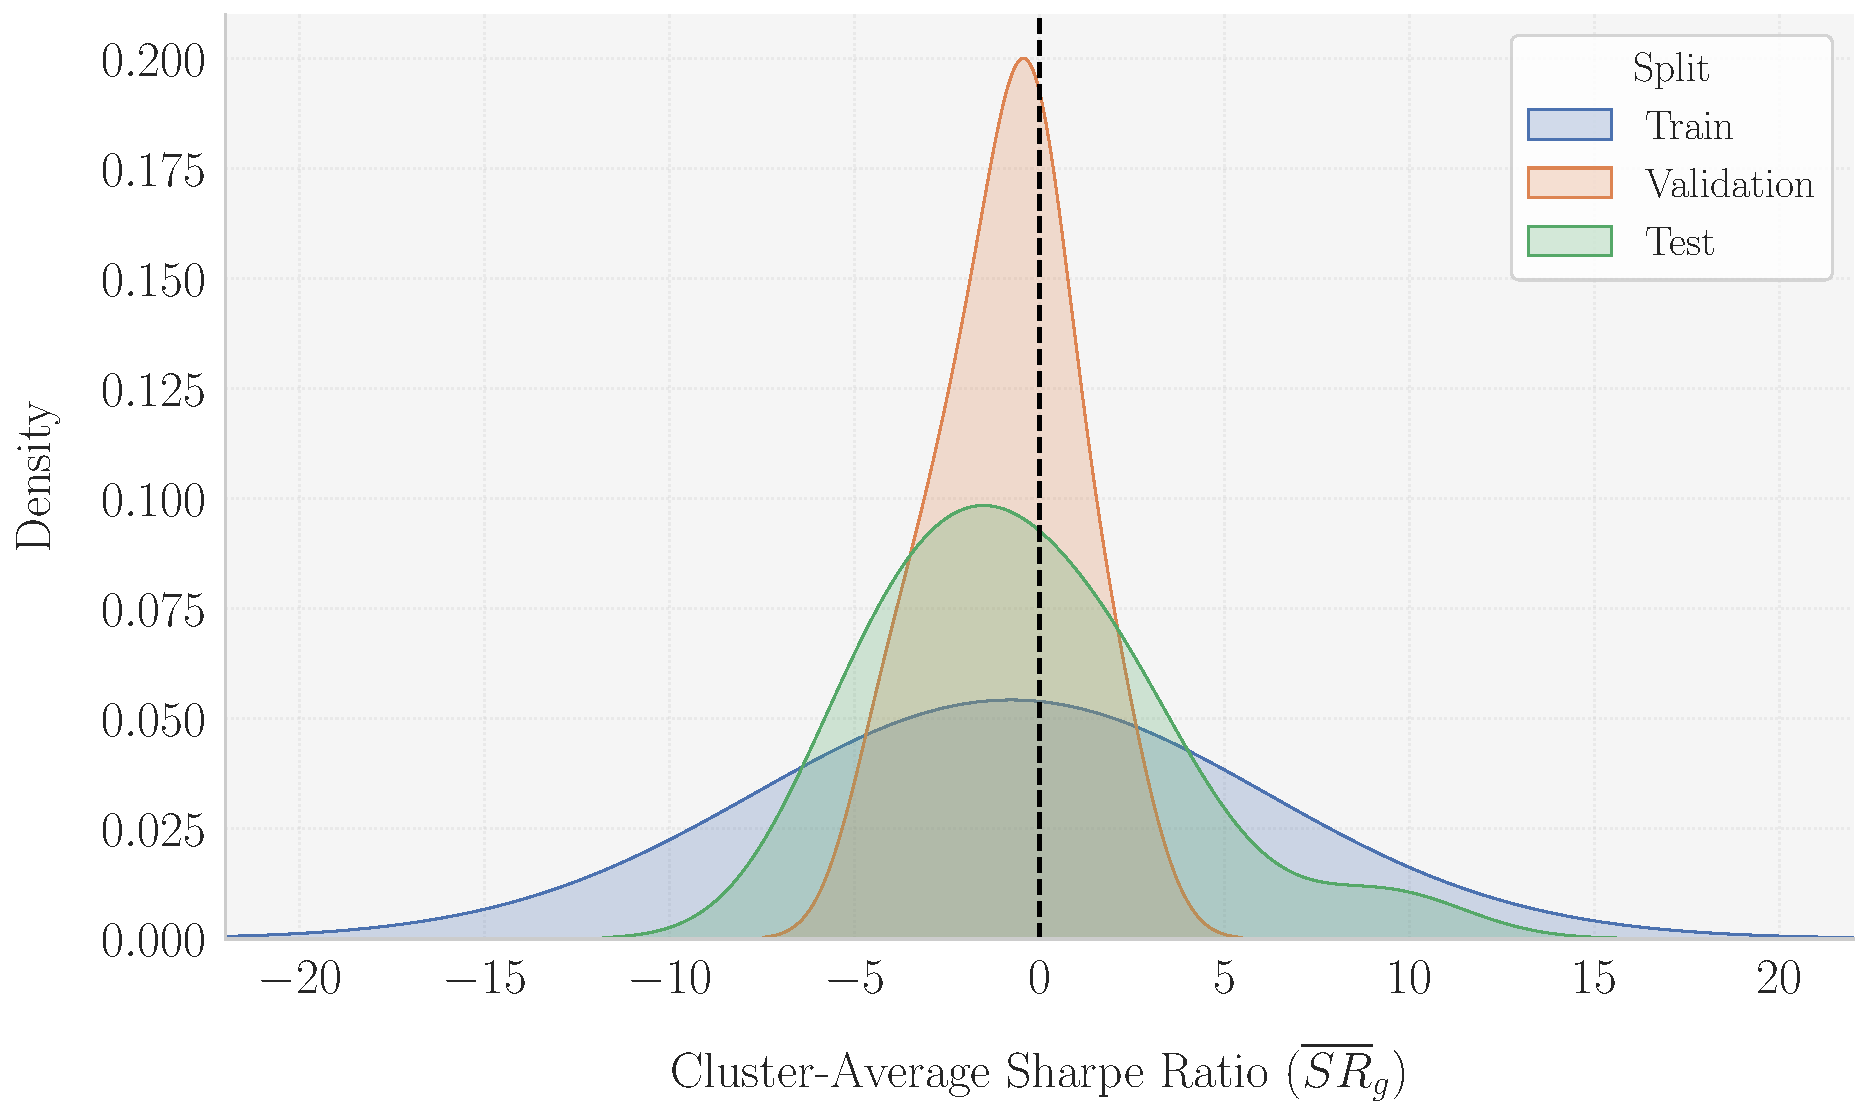
\includegraphics[scale=0.5]{fig_LLAMA_Cluster-Avg_SR_Distribution.pdf}
  \label{fig:LLM_cluster-average-SR-by-split}
 \subcaption*{\textit{Note: This figure presents the distribution of cluster-average Sharpe Ratios $(\overline{SR}_g)$ for the LLM-based clustering across the training, validation, and test data splits. All distributions exhibit left-skewness, indicating a higher frequency of lower Sharpe Ratios across clusters. The training data shows a distribution with fat tails, suggesting the presence of extreme values, while the validation data exhibits a much lighter-tailed distribution. In the test data, the distribution is more bell-shaped, with a notable concentration of Sharpe Ratios in the range of 5 to 15, indicating stronger performance in some clusters.}}

\end{figure}
%----------------------------------------------------

%%%%%%%%%%%%%%%%%%%%%%%%%%%%%%%%%%%%%%%%%%%%%%%%%%%%%
%%%%%%%%%%%%%%%%%   ALGORITHMS   %%%%%%%%%%%%%%%%%%%%
%%%%%%%%%%%%%%%%%%%%%%%%%%%%%%%%%%%%%%%%%%%%%%%%%%%%%
We now focus on developing two algorithms that optimally leverages the cluster information for our trading strategy. Our approach draws parallels with traditional portfolio sorting methods, where assets are typically arranged into deciles based on specific characteristics, and trading positions are established by going long on top deciles and short on bottom ones. Similarly, our strategy will construct self-financing portfolios based on clusters rather than individual assets: taking long positions in clusters expected to outperform and short positions in those expected to underperform.
%
To identify the optimal clusters for trading, we propose two distinct algorithmic approaches. The first approach, which we term \qquote{greedy}, selects clusters by maximizing the Sharpe Ratio within the validation dataset. The second approach, termed \qquote{stable}, utilizes a broader information set by incorporating both training and validation data, aiming to identify clusters that maintain consistent performance across different time periods. In both algorithms, we impose sign restrictions to ensure that our trading positions align with the expected direction of returns.

\subsubsection{Greedy Algorithm}

The greedy selection of clusters is done in the validation sample 
$
\mathcal{B}^{val}:= \{
(i,j)\in\mathcal{B} 
 \mid 
  i \in \D^{val} \}
~,
$
from where we compute the cluster-average $\overline{S R}_g^{val}$ for each $g\in\G$.
%
%----------------------------------------------------
Define $\mathcal G_{SR^+}^{val}:=\{ g\in \mathcal G \mid \overline{SR}_g^{val} >0\}$ and $\mathcal G_{SR^-}^{val}:=\{ g\in \mathcal G \mid \overline{SR}_g^{val} <0\}$ as the sets of clusters with positive and negative Sharpe Ratios in the validation sample. Obviously, we will be interested in taking long positions when reading an article that is clustered in some $g\in \mathcal G_{SR^+}^{val}$, and short positions in clusters $g\in \mathcal G_{SR^+}^{val}$. 

\mx 
%----------------------------------------------------
However, our trading strategy will not trade every cluster $g\in\G$. Instead, it will select the clusters from $\mathcal G_{SR^+}$ and $\mathcal G_{SR^-}$ that lead the to most profitable trades. 
To identify such clusters, we rank them by their average Sharpe Ratio. Define the ranking function $\mathfrak{R}: \mathcal{G} \to \3{1, \ldots, k^*}$ such that
$$
\mathfrak{R}_g^{val}
=
\sum_{h \in \mathcal{G}} 
\mathbf{1}\1{
\overline{S R}_h^{val} \geq \overline{S R}_g^{val} 
}
$$
where $\mathbf{1}(\cdot)$ is the indicator function which equals 1 if the condition inside is true and 0 otherwise.

\mx
%----------------------------------------------------
The number of traded clusters on either side (long and short) will be upper-bounded by some hyperparameter of our choice $\theta \in \mathbb{N}$
%$\theta \in \{2 m \mid m \in \mathbb{N}\}$ 
which we set proportional to the number of clusters. Namely, $\theta =\integer{\rho k}$ for some $\rho\in(0,1)$, which has been set to $\rho=0.5$ (this choice is justified in section A.2. of the Appendix).
%
The actual number of traded clusters will not be exactly $\theta$ as there is a natural bound coming from the cardinalities of $\mathcal G_{SR^+}$ and $\mathcal G_{SR^-}$. Hence, the actual number of long and short-traded clusters will be
$
\theta^+ := \min(\theta, ~|\mathcal G_{SR^+}|)
~\t{and}~
\theta^- := \min(\theta, ~|\mathcal G_{SR^-}|)
.
$
%----------------------------------------------------
The set of traded clusters $\mathcal G_{\theta}$ is defined as:
$$
\G_\theta := 
\3{
g \in \mathcal G 
\mid 
1\leq \mathfrak{R}_g^{val} \leq \theta^+
~\vee~ 
k^* -\theta^- < \mathfrak{R}_g^{val} \leq k^*
} 
= 
\G_{\theta}^+ \cup \G_{\theta}^-
~,
$$
where
$
\G_{\theta}^+ := 
\{ g \in\G \mid 
1\leq \mathfrak{R}_g^{val} \leq \theta^+
\}
$
is the set of long-traded clusters,
$
\G_{\theta}^- := 
\{ g \in\G \mid 
k^*-\theta^-
< \mathfrak{R}_g^{val} \leq 
k^*
\}
$
is the set of short-traded clusters 
and, clearly, $\abs{\G_{\theta}}=\theta^+ + \theta^- $.\footnote{
Alternatively, we could trade the same number of clusters in the long and short side by defining a unique 
$
\theta^* := \min\1{\theta, |\mathcal G_{SR^+}|, |\mathcal G_{SR^-}| }
%,
$
such that
$
\G_\theta := 
\3{
g \in \mathcal G 
\mid 
1\leq \mathfrak{R}_g^{val} \leq \theta^*
~\vee~ 
k^*-\theta^* < \mathfrak{R}_g^{val} \leq k^*
} 
$
and 
$\abs{\G_\theta}=2\theta^*$.
}
In the appendix, we can find the formal design of this algorithm (\cref{alg:greedy_selection}).

%%%%%%%%%%%%%%%%%%%%%%%%%%%%%%%%%%%%%%%%%%%%%%%%%%%%%
\subsubsection{Stable Algorithm}
%%%%%%%%%%%%%%%%%%%%%%%%%%%%%%%%%%%%%%%%%%%%%%%%%%%%%

In this case, we prioritize the stability of the cluster rankings by ensuring that the traded clusters minimize the rank difference of the cluster-average Sharpe Ratios between the training and validation samples. 
To begin, we compute the rank of each cluster based on the average Sharpe Ratios in both the training and validation samples. This delivers $\{\mathfrak{R}_g^{tr}\}_{g\in\G}$ and $\{\mathfrak{R}_g^{val}\}_{g\in\G}$, which provides a measure of the relative performance of the clusters within each sample.

\mx 
Next, we calculate the absolute difference in ranks between the training and validation samples for each cluster, which allows us to measure the stability of each cluster's performance between the two samples
%
$$
\delta_{g} := | \mathfrak{R}_{g}^{tr} - \mathfrak{R}_{g}^{val} |
~.
$$

Clusters are then sorted based on their rank differences $\delta_{g}$ in descending order. To do this, we can simply compute the ranking of the ranking differences as
$$
\mathfrak{R}(\delta_g) := \sum_{h\in\G} \mbf{1}\1{\delta_g \geq  \delta_h }
.
$$
Next, we select the top $2\theta\in\mathbb{N}$ clusters with the smallest rank differences, indicating the most stable clusters across the training and validation samples. The selected clusters now are
%denoted as $\mathcal{G}_{\theta}$
$$
\mathcal{G}_{\theta} = 
\3{
g\in\G \c 1 \leq \mathfrak{R}(\delta_g) \leq 2\theta 
}
.
$$

Finally, we determine the sets of long and short-traded clusters based on the average Sharpe Ratios in both the training and validation samples. In particular, the set of long-traded clusters ($\mathcal{G}_{\theta}^{+}$) are the ones that have positive average Sharpe Ratios in both, training and validation samples
$$
\mathcal{G}_{\theta}^{+} = \{g \in \mathcal{G}_{\theta} \mid \overline{SR}_{g}^{tr} > 0 ~\wedge~ \overline{SR}_{g}^{val} > 0\}
,
$$
and by symmetry, short-traded clusters ($\mathcal{G}_{\theta}^{-}$) are the ones that have negative average Sharpe Ratios in both, training and validation samples
$$
\mathcal{G}_{\theta}^{-} = \{g \in \mathcal{G}_{\theta} \mid \overline{SR}_{g}^{tr} < 0 ~\wedge~ \overline{SR}_{g}^{val} < 0\}
~.
$$


This approach ensures that we select the most stable clusters for trading, reducing the risk associated with rank variability between the training and validation samples, and ensuring that the direction of the signal is consistent across the two splits. The final output consists of the sets of long-traded and short-traded clusters, which are then used to implement the trading strategy.


The implementation of the algorithm is methodically presented in the Appendix (\cref{alg:rank_stability}).


%%%%%%%%%%%%%%%%%%%%%%%%%%%%%%%%%%%%%%%%%%%%%%%%%%%%%
%%%%%%%%%%%%%%%%%%   KMEANS   %%%%%%%%%%%%%%%%%%%%%%%
%%%%%%%%%%%%%%%%%%%%%%%%%%%%%%%%%%%%%%%%%%%%%%%%%%%%%
%----------------------------------------------------
\inserthere{tab:KMeans_Clusters_Signal}

\begin{table}[H]
\centering
{\fontsize{11}{12.5}\selectfont
\caption{Mapping of embeddings-based KMeans clusters to Trading Signals}
%\begin{tabular}{|c|L{13cm}|c|c|} 
\begin{tabular}{cL{13cm}cc} 
\hline \Xhline{2\arrayrulewidth}
%\rowcolor{gray!10}
\multicolumn{2}{c}{\textbf{Cluster}} & \textbf{Greedy} & \textbf{Stable} \\ \hline \Xhline{2\arrayrulewidth}
0 & Miscellaneous (Colonial, Acciona, Amadeus, Grifols, Endesa, IAG, Bankinter...) &  \textcolor{darkred}{\textsc{short}} &  \\ \hline
1 & Quarterly \& Semi-Annual Earnings Reports &  \textcolor{darkred}{\textsc{short}} &  \\ \hline
2 & BBVA \& Sabadell: Financial Performance \& Strategic Movements &  \textcolor{darkred}{\textsc{short}} &  \\ \hline
3 & Telef�nica \& Cellnex: Telecommunications Tower Sales \& Market Dynamics &  \textcolor{darkgreen}{\textsc{long}} & \textcolor{darkgreen}{\textsc{long}} \\ \hline
4 & CaixaBank: Mergers and Strategic Moves in the Banking Sector &   &  \\ \hline
5 & Telef�nica, Indra, \& M�sM�vil: Regulatory and Strategic Moves in Telecom &  \textcolor{darkgreen}{\textsc{long}} &  \\ \hline
6 & Siemens Gamesa: Supply Agreements, Profitability Targets in Renewable Energy &  \textcolor{darkred}{\textsc{short}} &  \\ \hline
7 & Cellnex: Strategic Acquisitions and Financial Moves in Telecom Infrastructure &  \textcolor{darkgreen}{\textsc{long}} &  \\ \hline
8 & Acciona, Endesa, Enag�s \& Naturgy: Strategic Moves \& Regulatory Developments in the Energy Sector &  \textcolor{darkgreen}{\textsc{long}} &  \\ \hline
9 & Repsol: Strategic Moves and Challenges in the Energy Sector &  \textcolor{darkgreen}{\textsc{long}} &  \\ \hline
10 & Ferrovial, Acciona: Strategic Expansions and Financial Maneuvers in Infrastructure &  \textcolor{darkred}{\textsc{short}} & \textcolor{darkred}{\textsc{short}} \\ \hline
11 & Solaria: Strategic Moves and Market Challenges in Renewable Energy &  \textcolor{darkgreen}{\textsc{long}} & \textcolor{darkgreen}{\textsc{long}} \\ \hline
12 & Iberdrola: Strategic Collaborations and Renewable Energy Developments &  \textcolor{darkred}{\textsc{short}} &  \\ \hline
13 & IAG: Financial Performance &  \textcolor{darkgreen}{\textsc{long}} &  \\ \hline
14 & Santander \& CaixaBank: Financial Moves and Sustainability Initiatives &  \textcolor{darkred}{\textsc{short}} &  \\ \hline
15 & ACS \& Acciona: Strategic Movements and Infrastructure Projects &  \textcolor{darkred}{\textsc{short}} & \textcolor{darkred}{\textsc{short}} \\ \hline
16 & Telef�nica: Financial Performance and Strategic Moves &  \textcolor{darkgreen}{\textsc{long}} &  \\ \hline
17 & Meli� and Spanish Tourism Sector: Challenges Amidst the Pandemic &  \textcolor{darkred}{\textsc{short}} &  \\ \hline
18 & Takeover Bids for Naturgy and M�sM�vil &  \textcolor{darkred}{\textsc{short}} &  \\ \hline
19 & Naturgy: Financial Performance &  \textcolor{darkred}{\textsc{short}} & \textcolor{darkred}{\textsc{short}} \\ \hline
20 & PharmaMar, Grifols: Regulatory Approvals and Market Moves in the Pharmaceutical Sector &  \textcolor{darkgreen}{\textsc{long}} & \textcolor{darkgreen}{\textsc{long}} \\ \hline
21 & Repsol: Financial Performance &  \textcolor{darkgreen}{\textsc{long}} & \textcolor{darkgreen}{\textsc{long}} \\ \hline
22 & Aena: Financial Performance &  \textcolor{darkgreen}{\textsc{long}} & \textcolor{darkgreen}{\textsc{long}} \\ \hline
23 & Enag�s, Endesa, Iberdrola, Red El�ctrica: Regulatory and Market Challenges in the Energy Sector &  \textcolor{darkred}{\textsc{short}} &  \\ \hline
24 & BBVA, CaixaBank, Banco Sabadell: Layoffs and Restructuring &  \textcolor{darkgreen}{\textsc{long}} & \textcolor{darkgreen}{\textsc{long}} \\ \hline
25 & Inditex, Acerinox: Market Performance and Strategic Developments in the Post-Covid Context &  \textcolor{darkred}{\textsc{short}} & \textcolor{darkred}{\textsc{short}} \\ \hline \Xhline{2\arrayrulewidth}
\end{tabular}
\label{tab:KMeans_Clusters_Signal}
}
\subcaption*{\textit{
{ Note: Mapping of embeddings-based KMeans clusters to their Trading Signal \textsc{(long/short)} for the two proposed cluster-selection algorithms (Greedy and Stable). The Greedy algorithm longs (shorts) clusters that maximize (minimize) the cluster-average-$SR$ in the validation sample subject to a positivity (negativity) constraint, while the Stable algorithm longs (shorts) clusters that minimize the rank difference between the training and validation rankings of the cluster-average-$SR$'s subject to a positivity (negativity) constraint, which is now imposed on both sample splits. In both algorithms, the cardinality of each leg is upper-bounded by a hyperparameter $\theta$. Cluster labels are proposed based on the articles they pool.
}
}}
\end{table}
%----------------------------------------------------
In Table \ref{tab:KMeans_Clusters_Signal} we show the 26 clusters with their proposed names (based on the articles they pool together as shown in \cref{tab:KMeans_Articles_3_English}) and the selection of long and short-traded clusters according to each algorithm: \qquote{greedy} and \qquote{stable}. We write ``\textsc{long}'' for those clusters $g\in\G_\theta^+$ and ``\textsc{short}'' for $g\in\G_\theta^-$. 
%
%\mx 
As we can see, trading clusters of news articles based on this procedure is quite risky, as there is a high reliance of the signal on the past performance of a cluster. For example, clusters 21 and 22 are linked to the financial performance of Repsol and Aena, respectively, during the training and validation samples. Evidently, the future performance of these firms can change, but the signal provided by the algorithm will still indicate ``\textsc{long}''. 
%
%\bx 
Additionally, some clusters are heavily built on specific events of the period of time they were constructed upon. For example, cluster 17 pools articles related to the challenges of the tourism industry in Spain in Covid times, and cluster 25 is related to the post-covid developments of Inditex and Acerinox. Thus, a clustering approach based on embeddings is not generalizable over time. As the world evolves, clusters become outdated and require constant recalibration to maintain their relevance and predictive power. Hence, any trading strategy based solely on historical cluster performance is likely to produce misguided trading signals over time 

%%%%%%%%%%%%%%%%%%%%%%%%%%%%%%%%%%%%%%%%%%%%%%%%%%%%%
%%%%%%%%%%%%%%%%%%%%%%%%%%%%%%%%%%%%%%%%%%%%%%%%%%%%%
%%%%%%%%%%%%%%%%%%%%   LLM   %%%%%%%%%%%%%%%%%%%%%%%%
%%%%%%%%%%%%%%%%%%%%%%%%%%%%%%%%%%%%%%%%%%%%%%%%%%%%%
%%%%%%%%%%%%%%%%%%%%%%%%%%%%%%%%%%%%%%%%%%%%%%%%%%%%%
%----------------------------------------------------
\inserthere{tab:LLM_cluster_mapping_extended}

\begin{table}[H]
\caption{Mapping of LLM-based clusters to Trading Signals}
\centering
%{\footnotesize
\begin{tabular}{C{1cm}lcc}
\hline \Xhline{2\arrayrulewidth}
%\rowcolor{gray!10}
 \multicolumn{2}{c}{\textbf{Cluster}} & \textbf{Greedy} & \textbf{Stable} \\ \hline \Xhline{2\arrayrulewidth} 
0 & {(demand, minor, positive)} &  &  \\ \hline
1 & {(demand, minor, negative)} &  & \textcolor{darkred}{\textsc{short}} \\ \hline
2 & {(demand, major, positive)} & \textcolor{darkred}{\textsc{short}} & \textcolor{darkred}{\textsc{short}} \\ \hline
3 & {(demand, major, negative)} & \textcolor{darkgreen}{\textsc{long}} & \textcolor{darkgreen}{\textsc{long}} \\ \hline
\Xhline{2\arrayrulewidth}
4 & {(supply, minor, positive)} & \textcolor{darkgreen}{\textsc{long}} &  \\ \hline
5 & {(supply, minor, negative)} & \textcolor{darkred}{\textsc{short}} &  \\ \hline
6 & {(supply, major, positive)} & \textcolor{darkgreen}{\textsc{long}} &  \\ \hline
7 & {(supply, major, negative)} & \textcolor{darkred}{\textsc{short}} &  \\ \hline
\Xhline{2\arrayrulewidth}
8 & {(financial, minor, positive)} & \textcolor{darkgreen}{\textsc{long}} & \textcolor{darkgreen}{\textsc{long}} \\ \hline
9 & {(financial, minor, negative)} &  & \textcolor{darkred}{\textsc{short}} \\ \hline
10 & {(financial, major, positive)} & \textcolor{darkgreen}{\textsc{long}} &  \\ \hline
11 & {(financial, major, negative)} & \textcolor{darkred}{\textsc{short}} &  \\ \hline
\Xhline{2\arrayrulewidth}
12 & {(technology, minor, positive)} & \textcolor{darkgreen}{\textsc{long}} &  \\ \hline
13 & {(technology, minor, negative)} &  &  \\ \hline
14 & {(technology, major, positive)} & \textcolor{darkred}{\textsc{short}} &  \\ \hline
15 & {(technology, major, negative)} &  &  \\ \hline
\Xhline{2\arrayrulewidth}
16 & {(policy, minor, positive)} & \textcolor{darkred}{\textsc{short}} & \textcolor{darkred}{\textsc{short}} \\ \hline
17 & {(policy, minor, negative)} & \textcolor{darkred}{\textsc{short}} & \textcolor{darkred}{\textsc{short}} \\ \hline
18 & {(policy, major, positive)} & \textcolor{darkred}{\textsc{short}} & \textcolor{darkred}{\textsc{short}} \\ \hline
19 & {(policy, major, negative)} & \textcolor{darkred}{\textsc{short}} & \textcolor{darkred}{\textsc{short}} \\ \hline
\Xhline{2\arrayrulewidth}
\end{tabular}
%}
\vspace{0.5cm}
\subcaption*{\textit{
Note: Mapping of LLM-based clusters to their Trading Signal \textsc{(long/short)} for the two proposed cluster-selection algorithms (Greedy and Stable). The Greedy algorithm longs (shorts) clusters that maximize (minimize) the cluster-average-$SR$ in the validation sample subject to a positivity (negativity) constraint, while the Stable algorithm longs (shorts) clusters that minimize the rank difference between the training and validation rankings of the cluster-average-$SR$'s subject to a positivity (negativity) constraint, which is now imposed on both sample splits. In both algorithms, the cardinality of each leg is upper-bounded by a hyperparameter $\theta$. Each cluster corresponds to a type of news-implied firm-specific shock identified by our LLM according to the function calling schema.
}}
\label{tab:LLM_cluster_mapping_extended}
\end{table}
%----------------------------------------------------
%\mx 
%\hspace{0.5cm}
In contrast, our LLM-based clustering methodology offers significant advantages by focusing on the fundamental nature of economic shocks rather than historical patterns. This approach provides more robust and generalizable signals that are less susceptible to temporal changes in market conditions. Moreover, unlike the black box nature of vector embeddings, our methodology offers transparency and interpretability in signal generation. This is evident in how the \textit{Greedy} algorithm's cluster selection closely aligns with the direction of economic shocks: negative shocks typically correspond to price decreases and positive shocks to increases. 

Looking at \cref{tab:LLM_cluster_mapping_extended}, we observe that both algorithms consistently short articles classified as policy shocks, regardless of direction, while going long on cluster 8, which contains approximately one-third of news articles (those categorized as undergoing financial minor and positive shocks). This consistent shorting of policy shocks likely reflects markets' general aversion to policy uncertainty, as policy changes - even positive ones - often create implementation uncertainty and take time for market participants to fully price in. Interestingly, both algorithms also exhibit seemingly counter-intuitive behavior by going long on negative major demand shocks and short on positive major demand shocks. This pattern might suggest a ``mean reversion'' expectation in the algorithms, where major demand shocks are viewed as temporary deviations that will eventually correct: negative shocks present buying opportunities, while positive shocks signal potential overvaluation.

%%%%%%%%%%%%%%%%%%%%%%%%%%%%%%%%%%%%%%%%%%%%%%%%%%%%%
\subsection{Trading Rule \& Portfolio Construction}
%%%%%%%%%%%%%%%%%%%%%%%%%%%%%%%%%%%%%%%%%%%%%%%%%%%%%
\hspace{0.5cm}For a given selection of clusters $\G_{\theta}^+$ and $\G_{\theta}^-$, we launch trades and hold them for $L\in\mathbb{N}$ trading days over a window $\mathcal H^i$.
%
Formally, the trading rule $TR_{{{L}},\theta}\angl{(i,j),d}$ for a pair $(i,j)\in\mathcal{B}$ at trading day ${d}\in\tilde{\mathfrak d}$ is 
%
%----------------------------------------------------
\begin{align*}
TR_{{{L}},\theta}\angl{(i,j),{d}} := \mycases{rllllll}{
+1
&\IF 
&
[
(i,j)\in\mathcal{B}_g
~\wedge~
g \in \G_{\theta}^+
]
~\wedge~
{d}\in \mathcal H^i
\\
0
&\IF
&
[
(i,j)\in\mathcal{B}_g
~\wedge~
g \not\in \G_\theta ~
]
~\vee~
{d}
\not\in \mathcal H^i
\\
-1
&\IF 
&
[
(i,j)\in\mathcal{B}_g
~\wedge~
g \in \G_{\theta}^-
]
~\wedge~
{d}
\in \mathcal H^i
}
~.
\end{align*}
%----------------------------------------------------

In this context, a portfolio is a collection of positions taken in a firm's stocks according to $TR_{{{L}},\theta}\angl{(i,j),{d}}$. In other words, it is the set of all $\angl{(i,j),{d}}$ for which a trade is executed. 
\begin{align*}
\mathcal P:= 
\3{\angl{(i,j),{d}} 
\c 
(i,j)\in\mathcal{B} 
~\wedge~
{d}\in \tilde{\mathfrak{d}}
~\wedge~
TR_{{{L}},\theta}\angl{(i,j),{d}} \neq 0
}
.
\end{align*}
The set of open positions on a particular day ${d}\in\tilde{\mathfrak d}$ is defined as
$$
\mathcal{P}_{ d}
:=
\3{
(i, j) \in \mathcal{B} 
\c 
T R_{L, \theta}\langle(i, j), {d}\rangle \neq 0 
}
,
$$
and the portfolio is rebalanced every day, so each position $(i, j)\in \mathcal{P}_{d}$ receives a weight that is inversely proportional to the total amount of open positions in that day (i.e. $1/|\mathcal{P}_{d}|$).\footnote{
Note that the cardinality of the set of open positions at day ${d}\in\tilde{\mathfrak d}$, denoted as $|\mathcal{P}_{d}|$, can be computed as the sum of the absolute values of the trading rule over all pairs $(i,j)\in\mathcal B$
 for a given trading day $d\in\tilde{\mathfrak{d}}$.
$$
|\mathcal{P}_{ d}|=\sum_{(i,j)\in\mathcal B}
\abs{
TR_{L, \theta}\angl{(i,j),  d}
}
~.
$$
}
This produces an equally-weighted rolling-portfolio similar to \cite{jegadeesh1993returns} and \cite{chan2003stock}.
The overlapping returns of the portfolio at $d\in\tilde{\mathfrak{d}}$ can be obtained as an average of the abnormal returns weighted by the trading rule, which determines the direction of each position (long or short), and scaled by the number of open positions in that day:
$$
r_{d}^{\mathcal{P}} 
:= 
\frac{1}{|\mathcal{P}_{d}|}
\sum_{(i, j), \in \mathcal{P}_{d}}
T R_{{{L}}, \theta}\angl{(i,j), {d}} 
\cdot 
AR_{{d}}^{(i,j)}
~.
$$

Finally, defining the mean portfolio return as
%----------------------------------------------------
$
\mu^{\mathcal{P}}:=
({1}/{|\tilde{\mathfrak{d}}|})
\sum_{\tilde{d} \in \tilde{\mathfrak{d}}} \ln (1+r_{\tilde{d}}^{\mathcal{P}})
$
and the associated standard deviation:
$ 
\sigma^{\mathcal{P}}
:=
\sqrt{
({1}/{|\tilde{\mathfrak{d}}|-1})
\sum_{\tilde{d} \in \tilde{\mathfrak{d}}}
[\ln
(1+r_{\tilde{d}}^{\mathcal{P}}
)-\mu^{\mathcal{P}}]^2} 
$
, we can obtain the annualized Sharpe Ratio of the portfolio as
$ SR^{\mathcal{P}} :=  \sqrt{252} ~
{\mu^{\mathcal{P}}}/{\sigma^{\mathcal{P}}} 
$.
%----------------------------------------------------


%%%%%%%%%%%%%%%%%%%%%%%%%%%%%%%%%%%%%%%%%%%%%%%%%%%%%
%%%%%%%%  Evaluating the Trading Strategy  %%%%%%%%%
%%%%%%%%%%%%%%%%%%%%%%%%%%%%%%%%%%%%%%%%%%%%%%%%%%%%%

\subsection{Evaluating the Trading Strategy}
\hspace{0.5cm}The trading strategy is evaluated in the test sample by applying $TR\angl{(i,j),d}$ to all $(i,j)\in\mathcal{B}^{test}$. 
This delivers the portfolio
\begin{align*}
\mathcal{P}^{test}=\3{\angl{(i,j),d} \c (i,j)\in \mathcal{B}^{test} ~\wedge~  TR_{L,\theta}\angl{(i,j),d} \neq 0 }
,
\end{align*}
from where we can compute the portfolio returns 
$
r_{d}^{\mathcal{P}^{test}} = 
({1}/{|\mathcal{P}_{d}^{test}|})
\sum_{(i, j), \in \mathcal{P}_{d}^{test}}
T R_{{{L}}, \theta}\angl{(i,j), {d}} 
\cdot 
AR_{{d}}^{(i,j)}
,
$
and then obtain $\mu^{\mathcal{P}^{test}}$ and $\sigma^{\mathcal{P}^{test}}$. Finally, we evaluate the \textit{out-of-sample} performance of our trading strategy by looking at the Sharpe Ratio in the test sample
$
SR^{\mathcal{P}^{test}} = 
\sqrt{252}~
{\mu^{\mathcal{P}^{test}}}/{\sigma^{\mathcal{P}^{test}}}
.$

\mx 
In \cref{fig:KMeans_Portfolio_Cum_Returns} we plot the cumulative returns of the portfolio constructed based on our KMeans clustering of embeddings. In \cref{tab:KMeans_portfolio_statistics} we summarize the usual portfolio statistics. As we can see, both algorithms work well on the data splits they were trained on: the Stable algorithm works well on both, training and validation data, while the Greedy algorithm does a good job only on validation data as expected. However, this doesn't say anything about any of these algorithms, as it is easy to make profitable trades \textit{in-sample}. 
%
%\mx 
The generalizability of the strategy is determined \textit{out-of-sample} in the test data. As we can see, the performance is much worse there for both algorithms. In the plot, we can see that none of them is able to generate a consistent profile of earnings, and the statistics confirm that profits are negligible, and would most likely be eaten away by exogenous considerations such as trading costs and slippage.

%----------------------- PLOT ----------------------
\inserthere{fig:KMeans_Portfolio_Cum_Returns}
\begin{figure}[H]
  \centering
    \caption{Cumulative Returns of $\mathcal{P}_{\t{KMeans}}$ across data splits for embeddings-based clustering}
  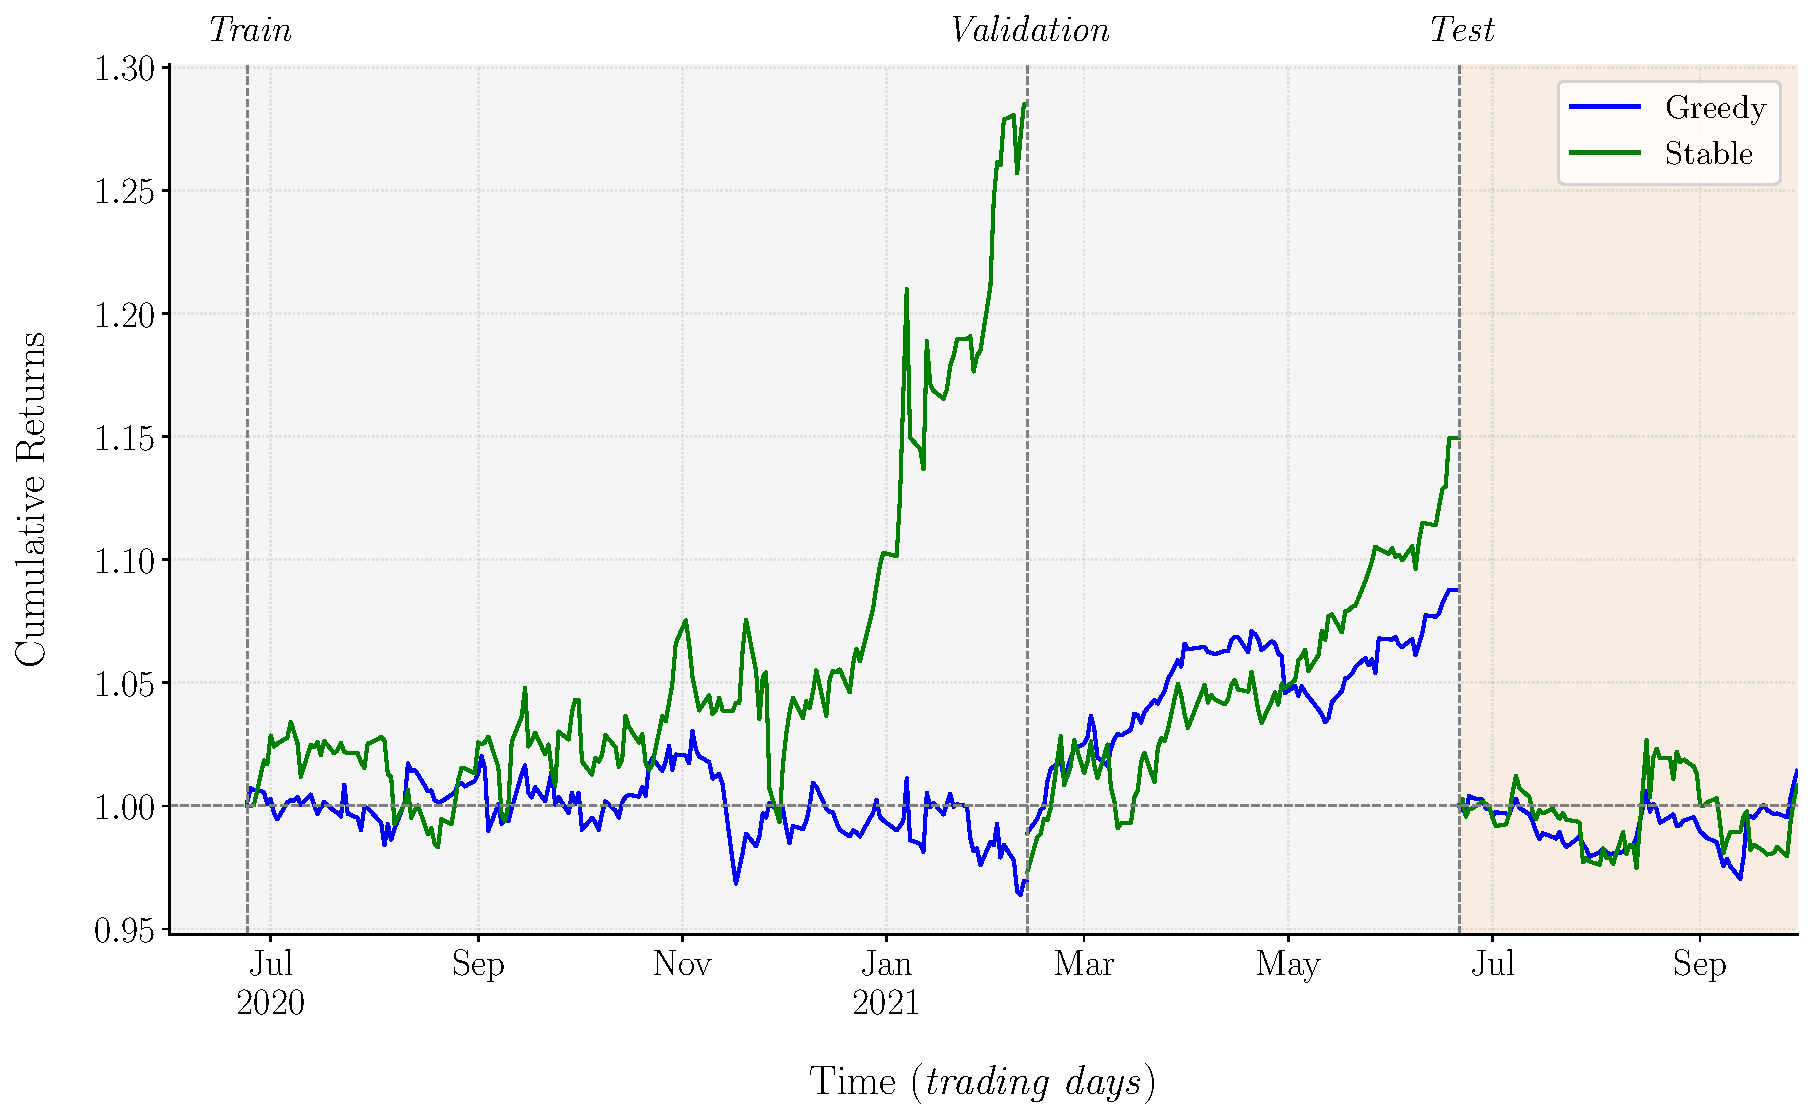
\includegraphics[scale=0.58]{fig_KMeans_Portfolio_Cum_Returns_(L=4,theta=0.5k).pdf}
  \subcaption*{\textit{Note: The holding period of the beta-neutral strategies is set to $L$ = 4 trading days and the number of traded clusters is, $\theta = \integer{0.5k}=13$ as we have $k^*=26$ clusters. The selection criteria for these parameters is based on maximizing the Sharpe Ratios of the train and validation samples. The poor out-of-sample performance of the trading strategy indicates that the embeddings-based clusters lack robustness and fail to generalize effectively over time.}}
  \label{fig:KMeans_Portfolio_Cum_Returns}
\end{figure}
%----------------------------------------------------
%----------------------------------------------------
\inserthere{tab:KMeans_portfolio_statistics}

\begin{table}[H]
    \caption{Statistics of $\mathcal{P}_{\t{KMeans}}$ across data splits}
    \centering
    \renewcommand{\arraystretch}{0.8}
%    \begin{tabular}{|c|c|c|c|c|c|}
    \begin{tabular}{cccccc}
    	\hline \Xhline{2\arrayrulewidth}
%        \rowcolor{gray!10}
        \textbf{Split} & \textbf{Algorithm} & \textbf{Cum. Return} & \textbf{Avg. Return} & \textbf{St. Deviation} & \textbf{Sharpe Ratio} \\
%        \rowcolor{gray!10}
        & & & \textit{(daily)} & \textit{(daily)} & \textit{(annual)} \\
        \hline \Xhline{2\arrayrulewidth}
        \multirow{2}{*}{All}       & \textit{Greedy} & 1.070 & 0.021 & 0.006 & 0.54 \\        & \textit{Stable} & 1.489 & 0.121 & 0.011 & 1.82 \\         \hline          \multirow{2}{*}{Train}       & \textit{Greedy} & 0.969 & -0.019 & 0.007 & -0.41 \\        & \textit{Stable} & 1.285 & 0.151 & 0.012 & 1.97 \\         \hline          \multirow{2}{*}{Validation}       & \textit{Greedy} & 1.088 & 0.094 & 0.005 & 3.23 \\        & \textit{Stable} & 1.149 & 0.155 & 0.008 & 2.93 \\         \hline          \multirow{2}{*}{Test}       & \textit{Greedy} & 1.014 & 0.019 & 0.004 & 0.70 \\        & \textit{Stable} & 1.008 & 0.011 & 0.009 & 0.20 \\         \hline \Xhline{2\arrayrulewidth}
    \end{tabular}
    \label{tab:KMeans_portfolio_statistics}
\vspace{0.5cm}
\subcaption*{\textit{Note: Portfolio statistics of the trading strategy based on clusters obtained from applying KMeans to article embeddings. The statistics provided are: Cumulative Return, Average Return, Standard Deviation and Sharpe Ratio, which have been computed in accordance to the formulas provided in the text. Such statistics are provided for both cluster-selection algorithms: Greedy and Stable. The Greedy algorithm longs (shorts) clusters that maximize (minimize) the cluster-average-$SR$ in the validation sample subject to a positivity (negativity) constraint, while the Stable algorithm longs (shorts) clusters that minimize the rank difference between the training and validation rankings of the cluster-average-$SR$'s subject to a positivity (negativity) constraint, which is now imposed on both sample splits. In both algorithms, the cardinality of each leg is upper-bounded by a hyperparameter $\theta$. 
The holding period of the beta-neutral positions is set to $L$ = 4 trading days and the number of traded clusters is, $\theta = 0.5k=13$ as there are $k^*=26$ KMeans clusters of article embeddings. The selection criteria for these hyperparameters ($L,\theta$) is based on maximizing the Sharpe Ratios of the train and validation samples.
} }
\end{table}
%----------------------------------------------------

%%%%%%%%%%%%%%%%%%%%%%%%%%%%%%%%%%%%%%%%%%%%%%%%%%%%%
%%%%%%%%%%%%%%%%%%%%%%%%%%%%%%%%%%%%%%%%%%%%%%%%%%%%%
%%%%%%%%%%%%%%%%%%%%%  LLM  %%%%%%%%%%%%%%%%%%%%%%%%%
%%%%%%%%%%%%%%%%%%%%%%%%%%%%%%%%%%%%%%%%%%%%%%%%%%%%%
%%%%%%%%%%%%%%%%%%%%%%%%%%%%%%%%%%%%%%%%%%%%%%%%%%%%%

\mx 
In \cref{fig:LLM_portfolio_returns} we plot the cumulative returns of the portfolio based on LLM clustering ($\mathcal P_{LLM}$). As before, both algorithms perform really well on ``seen'' data. However, different from before, the \textit{Greedy} algorithm works well also on the Training Split (which it was not trained on). More importantly, both algorithms do a great job in the test data. As we can see, both are able to achieve a consistent profile of earnings through the split. 
%
The summary statistics of the portfolio are provided in \cref{tab:LLM_portfolio_statistics}, where we see confirmed the fact that both algorithms excel at anticipating the market out of sample. 

%----------------------- PLOT ----------------------
\inserthere{fig:LLM_portfolio_returns}
\begin{figure}[H]
  \centering
    \caption{Cumulative Returns of $\mathcal P_{LLM}$ across data splits for LLM-based clustering}
  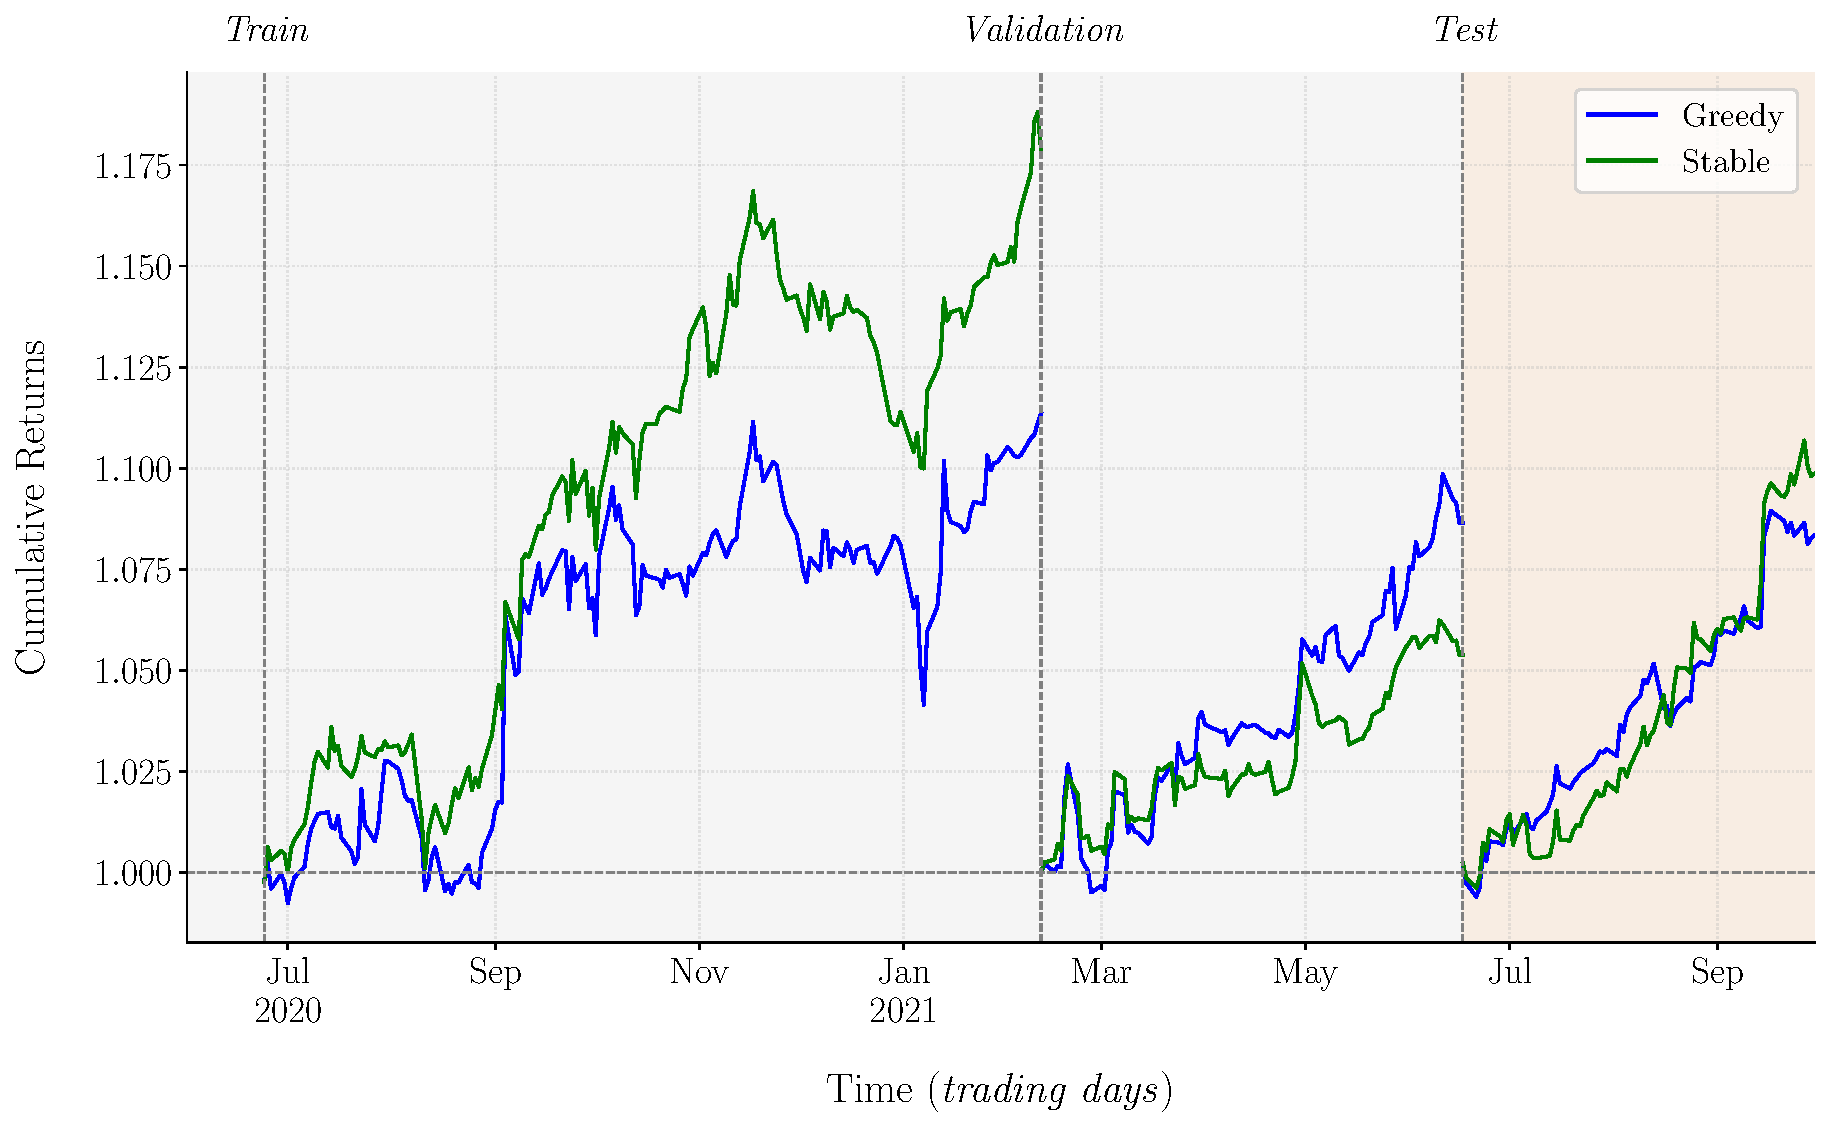
\includegraphics[scale=0.58]{fig_LLAMA_Portfolio_Cum_Returns_(L=4,theta=0.5k).pdf}
  \subcaption*{\textit{Note: The holding period of the beta-neutral strategies is set to $L=4$ trading days and the number of traded clusters is  $\theta=\integer{0.5k}=10$, as now we have $k=20$ clusters. The selection criteria for these parameters is based on maximizing the Sharpe Ratios of the train and validation samples. 
%
The strong out-of-sample performance of the trading strategy suggests that our proposed LLM-based clusters effectively provide insights for predicting market reactions to firm-specific economic shocks implied by news.
}}
  \label{fig:LLM_portfolio_returns}
\end{figure}
%----------------------------------------------------

%--------------------- TABLE ------------------------
\inserthere{tab:LLM_portfolio_statistics}

\begin{table}[H]
    \caption{Statistics of $\mathcal{P}_{LLM}$ across data splits}
    \centering
    \renewcommand{\arraystretch}{0.8}
    \begin{tabular}{cccccc}
        \hline \Xhline{2\arrayrulewidth}
%        \rowcolor{gray!10}
        \textbf{Split} & \textbf{Algorithm} & \textbf{Cum. Return} & \textbf{Avg. Return} & \textbf{St. Deviation} & \textbf{Sharpe Ratio} \\
%        \rowcolor{gray!10}
        & & & \textit{(daily)} & \textit{(daily)} & \textit{(annual)} \\
		\hline \Xhline{2\arrayrulewidth}
        \multirow{2}{*}{All}       & \textit{Greedy} & 1.311 & 0.082 & 0.006 & 2.17 \\        & \textit{Stable} & 1.365 & 0.095 & 0.005 & 2.78 \\         \hline          \multirow{2}{*}{Train}       & \textit{Greedy} & 1.113 & 0.065 & 0.007 & 1.44 \\        & \textit{Stable} & 1.179 & 0.100 & 0.006 & 2.53 \\         \hline          \multirow{2}{*}{Validation}       & \textit{Greedy} & 1.086 & 0.093 & 0.005 & 2.86 \\        & \textit{Stable} & 1.054 & 0.059 & 0.004 & 2.16 \\         \hline          \multirow{2}{*}{Test}       & \textit{Greedy} & 1.083 & 0.105 & 0.004 & 4.30 \\        & \textit{Stable} & 1.099 & 0.124 & 0.004 & 4.38 \\         \hline \Xhline{2\arrayrulewidth}
    \end{tabular}
    \label{tab:LLM_portfolio_statistics}
\vspace{0.5cm}
\subcaption*{\textit{Note: Portfolio statistics of the trading strategy applied to the LLM clusters. The statistics provided are: Cumulative Return, Average Return, Standard Deviation and Sharpe Ratio, which have been computed in accordance to the formulas provided in the text. Such statistics are provided for both cluster-selection algorithms: Greedy and Stable. The Greedy algorithm longs (shorts) clusters that maximize (minimize) the cluster-average-$SR$ in the validation sample subject to a positivity (negativity) constraint, while the Stable algorithm longs (shorts) clusters that minimize the rank difference between the training and validation rankings of the cluster-average-$SR$'s subject to a positivity (negativity) constraint, which is now imposed on both sample splits. In both algorithms, the cardinality of each leg is upper-bounded by a hyperparameter $\theta$. 
The holding period of the beta-neutral positions is set to $L$ = 4 trading days and the number of traded clusters is, $\theta = 0.5k=13$ as there are $k^*=26$ KMeans clusters of article embeddings. The selection criteria for these hyperparameters ($L,\theta$) is based on maximizing the Sharpe Ratios of the train and validation samples.
}}
\end{table}
%----------------------------------------------------



%%%%%%%%%%%%% ROBUSTNESS CHECKS %%%%%%%%%%%%%%%%%%

\section{Robustness Checks}

\hspace{0.5cm} In our applications we have worked with a holding window length of $L=4$ trading days and an upper bound on traded clusters of $\theta=\integer{0.5k}$. As shown in section A.2 of the Appendix, such choices result from the maximization of the Sharpe Ratios in the train and validation samples. All that is left is to check whether our out-of-sample results are sensitive to the choice of hyperparameters ($L,\theta$). For this purpose, we evaluate the variability of the Sharpe Ratios of the test portfolio ($SR^{\mathcal P^{test}}$) to changes in $L$ and $\theta$. 

\bx 
First, we focus on the holding period length of the beta-neutral strategy ($L$). For this purpose, we fix $\theta=\integer{0.5k}$ and, for each clustering method, obtain the series of Sharpe Ratios over a grid $\mbf L$ (which ranges from 1 to 20 trading periods). This delivers the series $\{SR^{\mathcal P ^{test}} (L)\}_{L\in\mbf L}$, which we then plot in two formats. On the left side of \cref{fig:LLM_Robustness_L} we plot the distribution of Sharpe Ratios in the grid, and in the right side, we show the mapping $L\mapsto SR^{\mathcal P ^{test}} (L)$ over $\mbf L$. 

%----------------------------------------------------
\inserthere{fig:LLM_Robustness_L}
\begin{figure}[H]
  \centering
  \caption{Sensitivity of $SR^{\mathcal P^{test}}$ to the holding window length ($L$)}
    \begin{subfigure}[b]{0.44\textwidth}
    \centering
    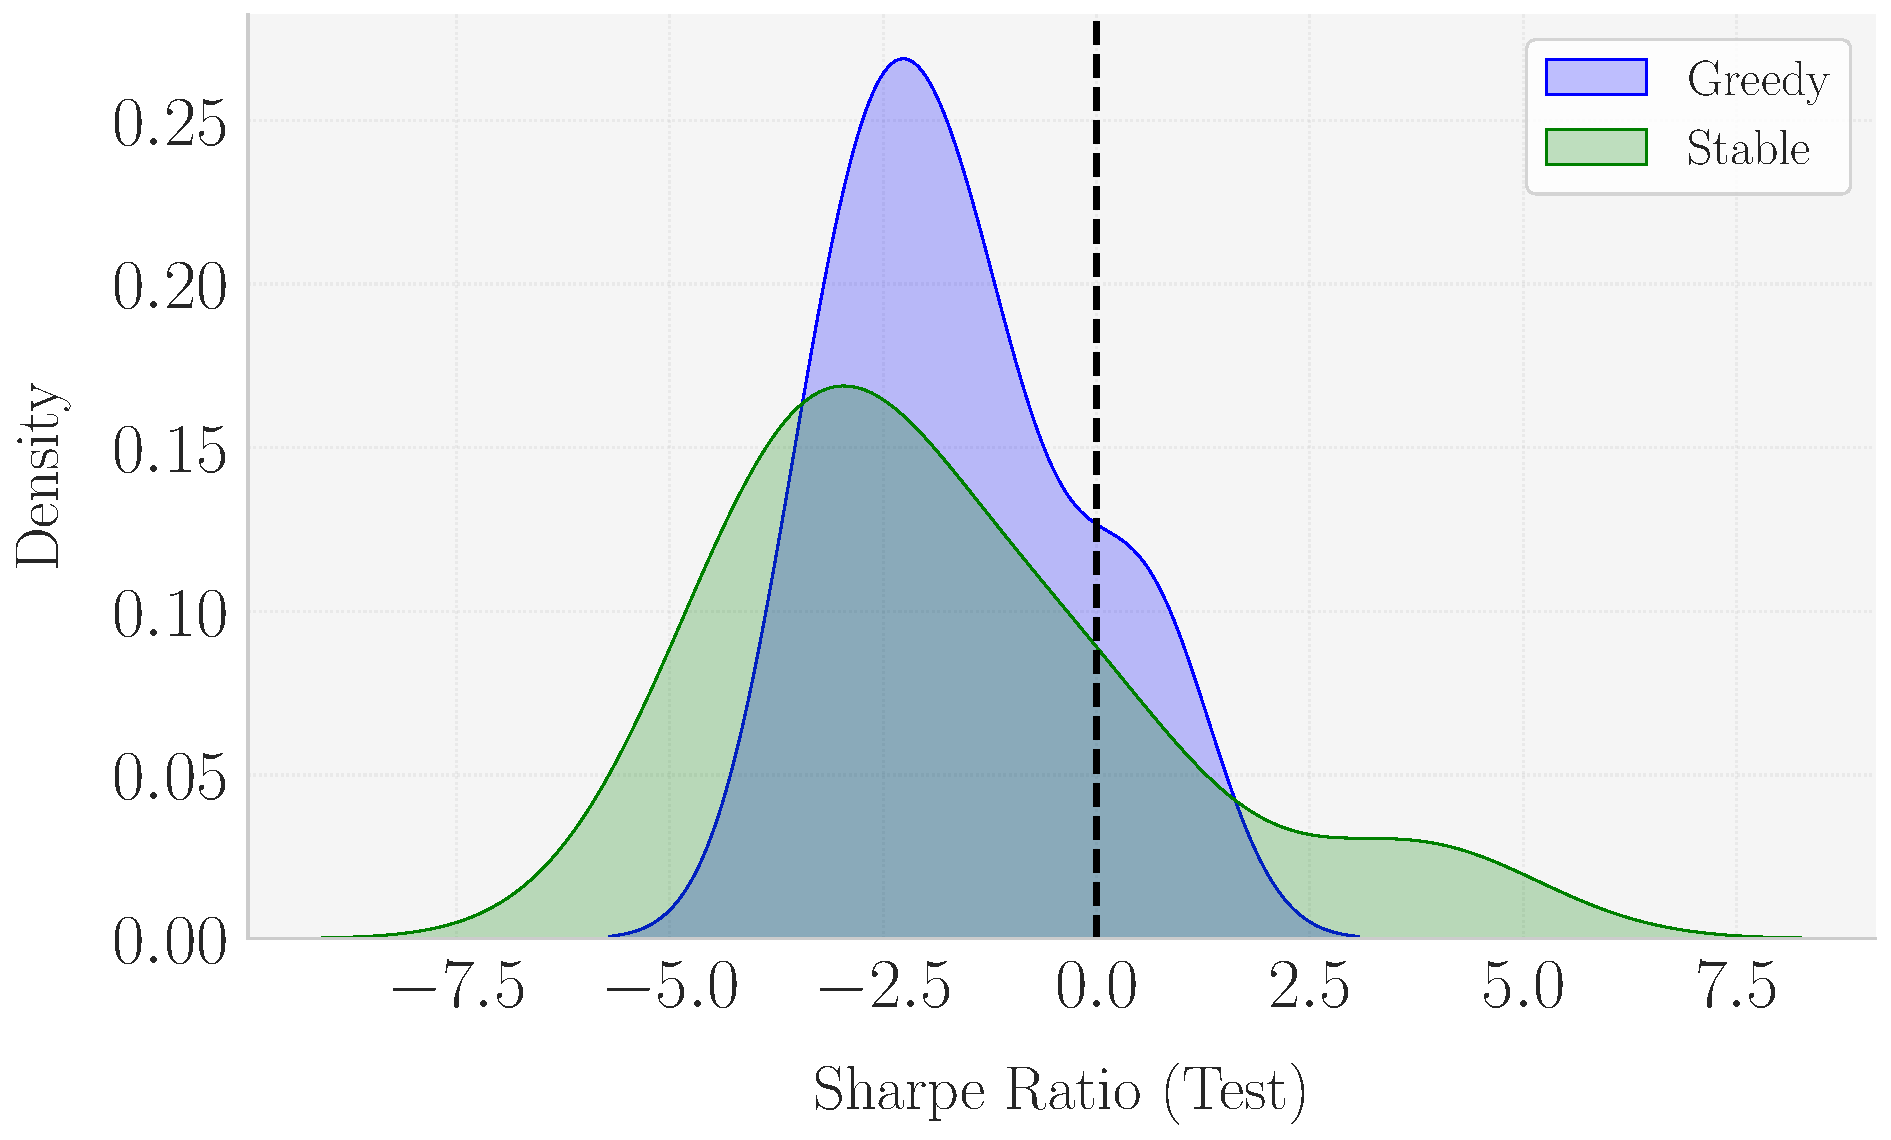
\includegraphics[width=\textwidth]{/Users/jesusvillotamiranda/Library/CloudStorage/OneDrive-UniversidaddeLaRioja/CEMFI/__MSc__/__Second_year__/6th_Term/MasterThesis/__Output/KMeans_RobustnessCheck_SR_Test_Set_Distribution_[Change_L].pdf}
    \caption{\textbf{KMeans}: Distribution of $SR^{\mathcal P^{test}}(L)$}
    \label{fig:KMeans_Robustness_L_Distr}
  \end{subfigure}
  \hspace{0.05\textwidth} % Add horizontal space between the subfigures
  \begin{subfigure}[b]{0.44\textwidth}
    \centering
    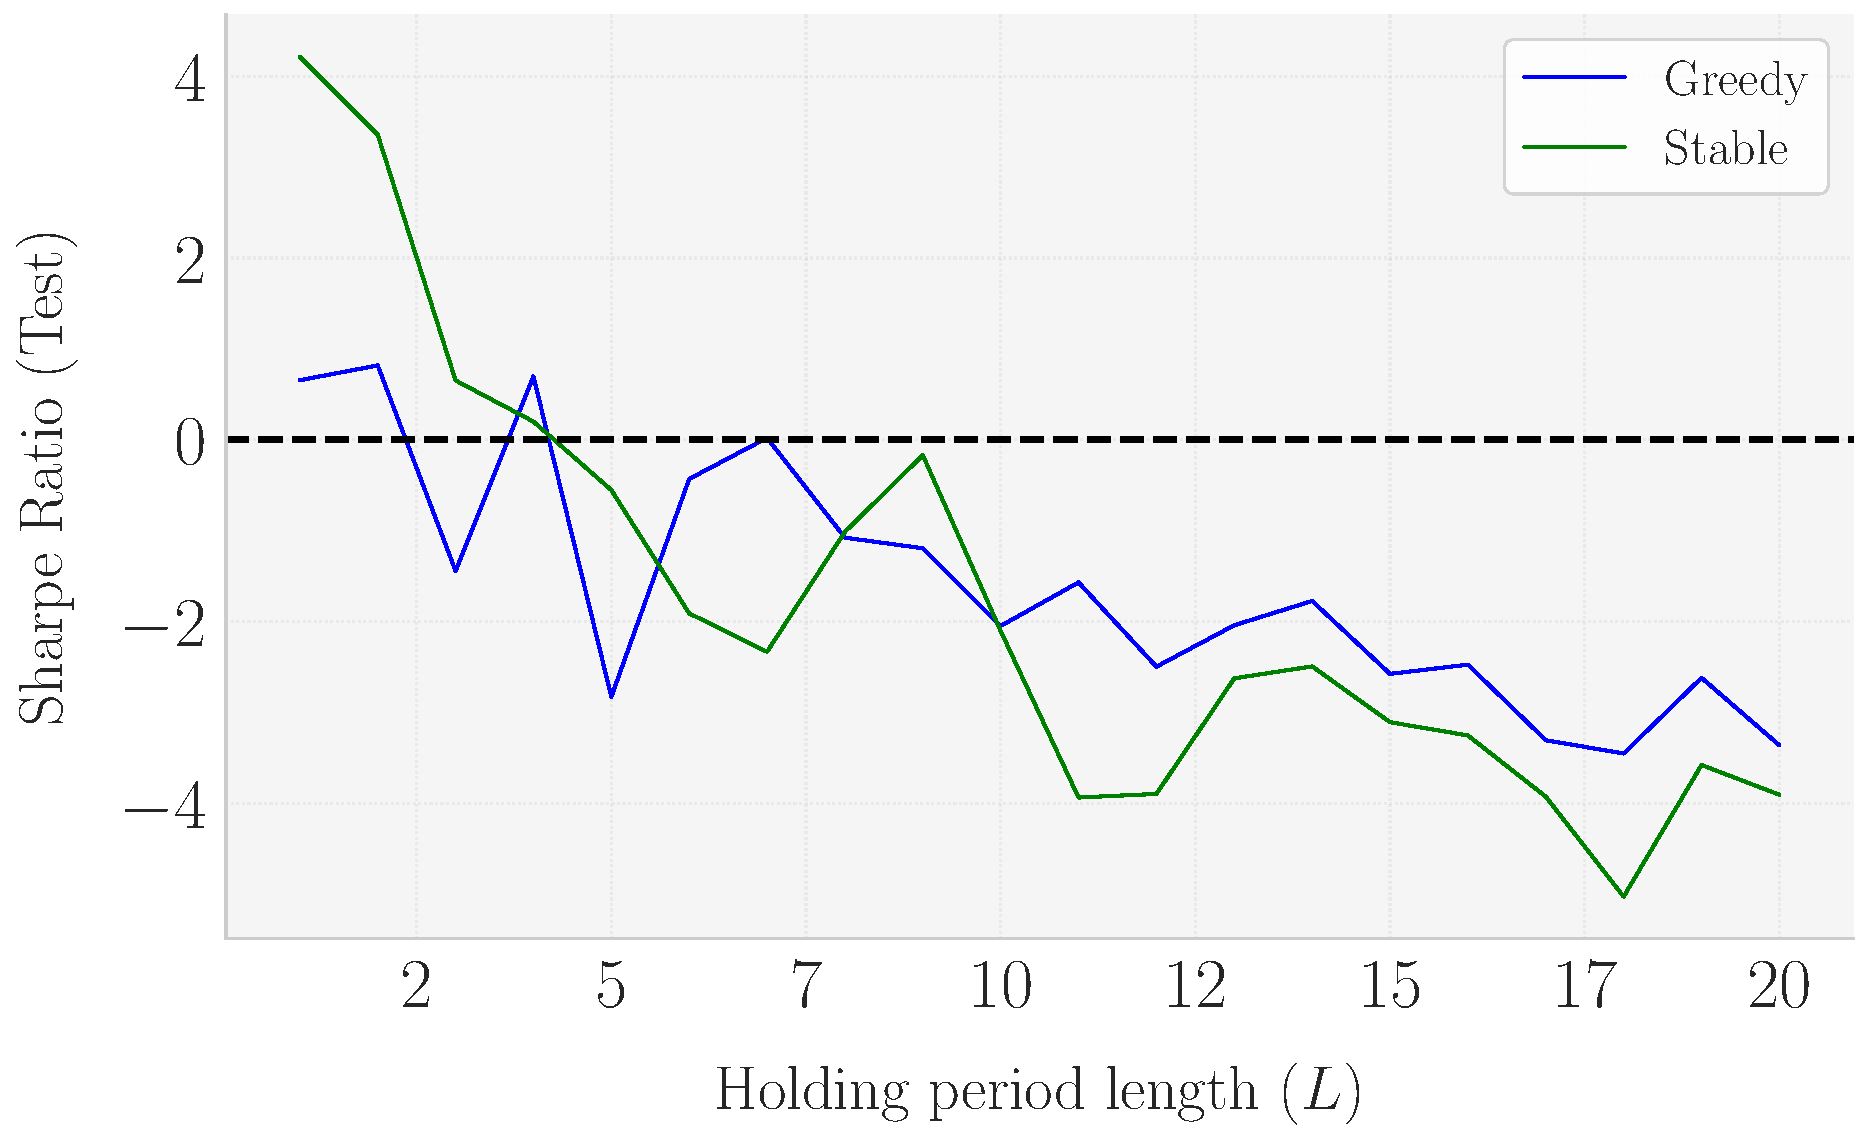
\includegraphics[width=\textwidth]{/Users/jesusvillotamiranda/Library/CloudStorage/OneDrive-UniversidaddeLaRioja/CEMFI/__MSc__/__Second_year__/6th_Term/MasterThesis/__Output/KMeans_RobustnessCheck_SR_Test_Set_vs_L_[Change_L].pdf}
    \caption{\textbf{KMeans}: Series of $SR^{\mathcal P^{test}}(L)$}
    \label{fig:KMeans_Robustness_L_Series}
  \end{subfigure}
  
  \bx 
      \begin{subfigure}[b]{0.44\textwidth}
    \centering
    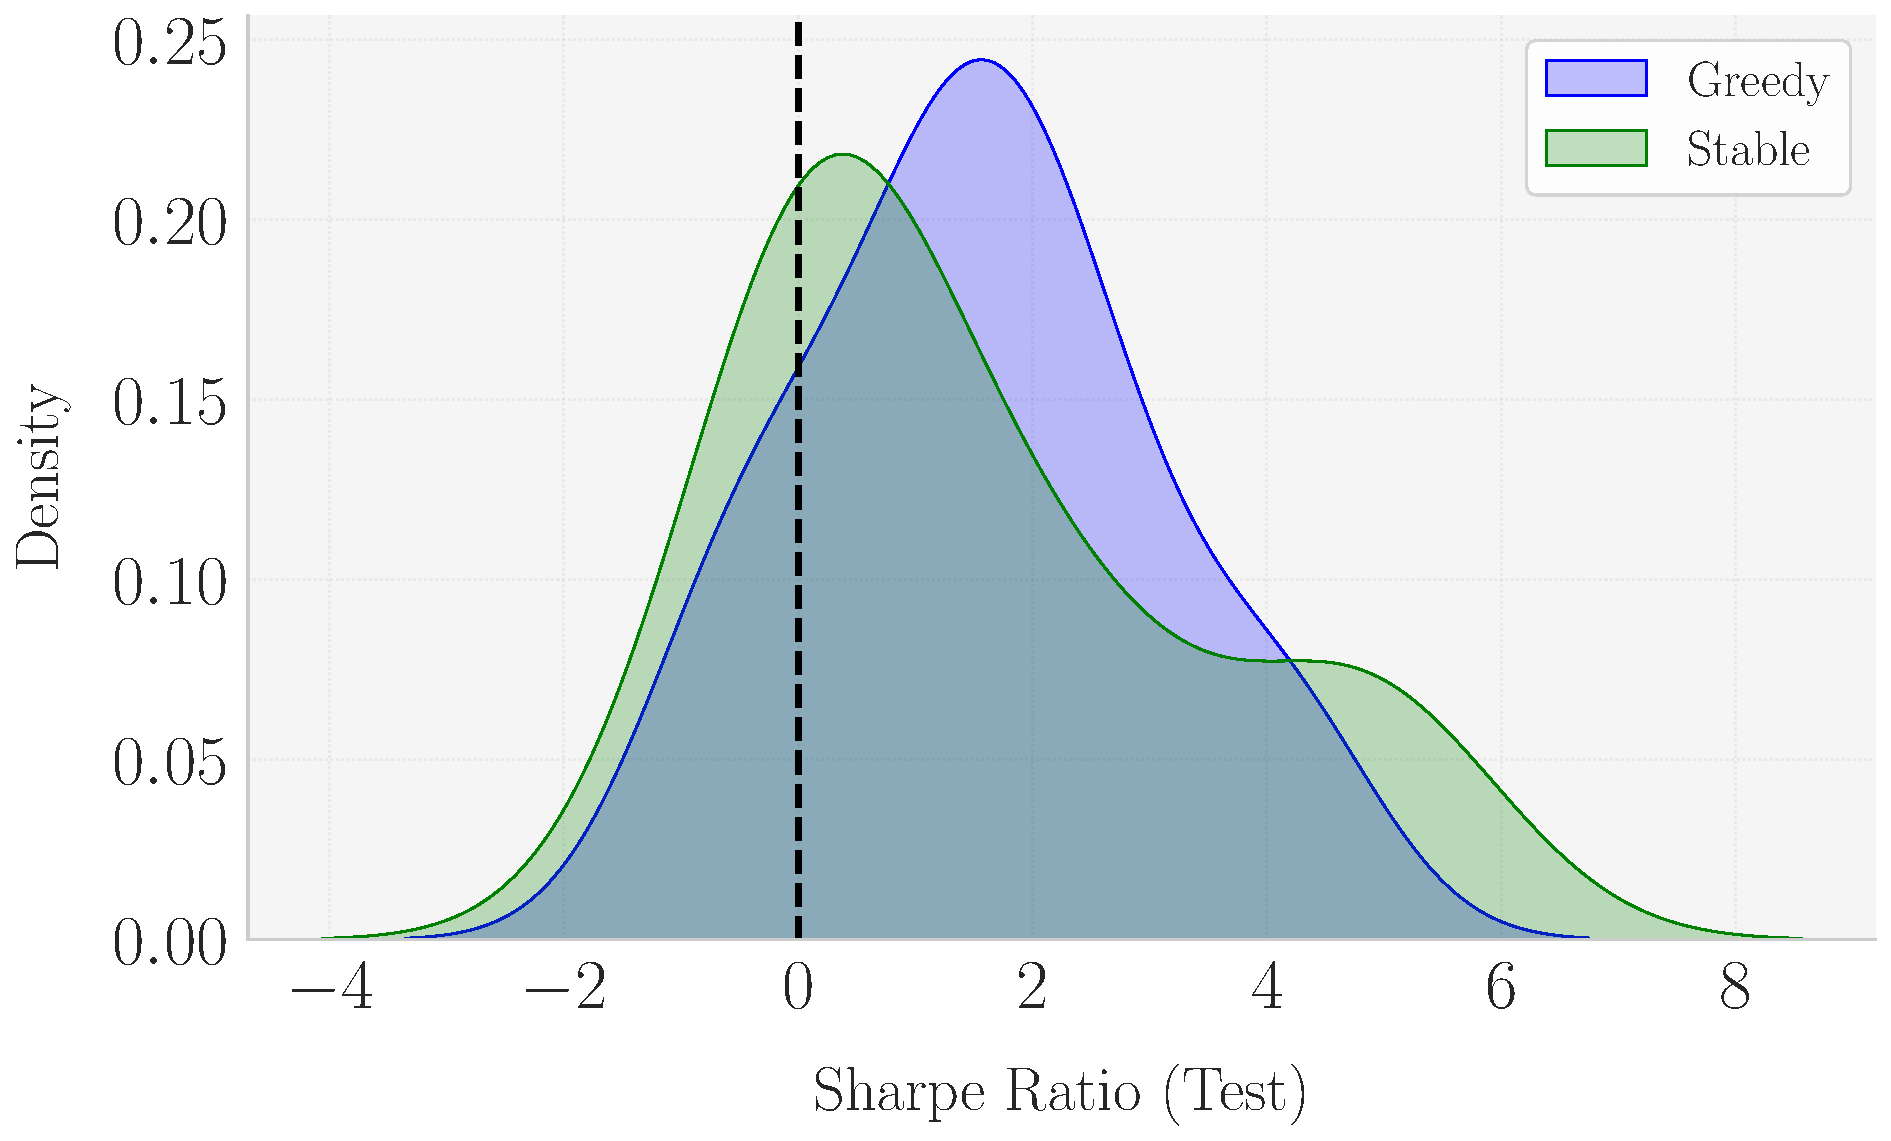
\includegraphics[width=\textwidth]{/Users/jesusvillotamiranda/Library/CloudStorage/OneDrive-UniversidaddeLaRioja/CEMFI/__MSc__/__Second_year__/6th_Term/MasterThesis/__Output/LLAMA_RobustnessCheck_SR_Test_Set_Distribution_[Change_L].pdf}
    \caption{\textbf{LLM}: Distribution of $SR^{\mathcal P^{test}}(L)$}
    \label{fig:LLM_Robustness_L_Distr}
  \end{subfigure}
  \hspace{0.05\textwidth} % Add horizontal space between the subfigures
  \begin{subfigure}[b]{0.44\textwidth}
    \centering
    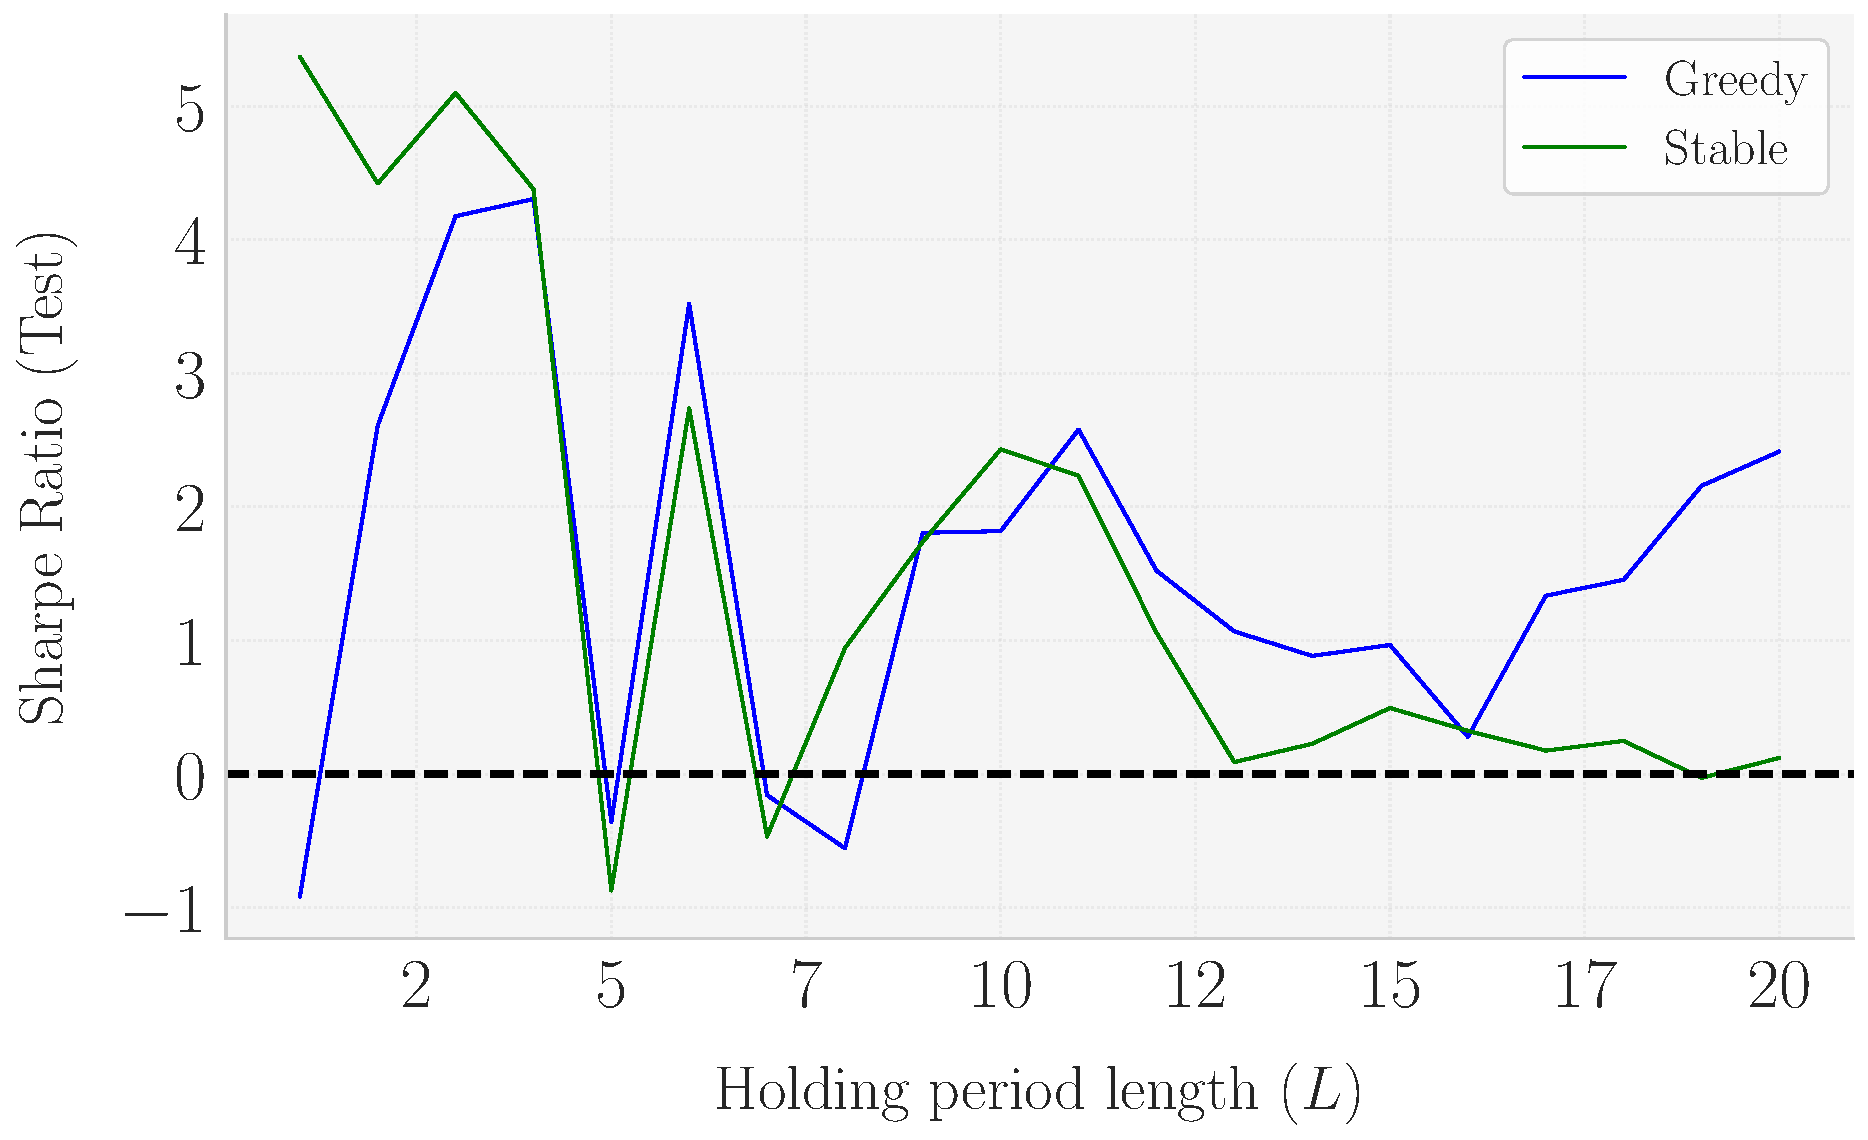
\includegraphics[width=\textwidth]{/Users/jesusvillotamiranda/Library/CloudStorage/OneDrive-UniversidaddeLaRioja/CEMFI/__MSc__/__Second_year__/6th_Term/MasterThesis/__Output/LLAMA_RobustnessCheck_SR_Test_Set_vs_L_[Change_L].pdf}
    \caption{\textbf{LLM}: Series of $SR^{\mathcal P^{test}}(L)$}
    \label{fig:LLM_Robustness_L_Series}
  \end{subfigure}
\label{fig:LLM_Robustness_L}
\mx 
\subcaption*{\textit{Note: This figure examines the sensitivity of the Sharpe Ratios ($SR^{\mathcal P^{test}}$) of the test portfolio to changes in the holding window length ($L$), with $\theta$ fixed at $\integer{0.5k}$. Panels \textsc{(a)} and \textsc{(b)} display the distribution and time series of $SR^{\mathcal P^{test}}(L)$ for KMeans clustering, respectively, while Panels \textsc{(c)} and \textsc{(d)} present the same for the LLM-based clustering. The left-hand panels show the skewness of the distributions: KMeans clustering results in a left-skewed distribution of Sharpe Ratios, whereas the LLM-based approach yields a right-skewed distribution, indicating higher profitability. The right-hand panels highlight that KMeans clustering only produces positive Sharpe Ratios for very short holding periods, whereas the LLM-based clustering shows more consistent positive performance across a wider range of $L$ values, though with some variability.}}
\end{figure}
%----------------------------------------------------

From \cref{fig:KMeans_Robustness_L_Distr} it follows that KMeans clustering produces a distribution that is clearly left-skewed, while the distribution of $SR^{\mathcal P ^{test}}$ for LLM clustering is clearly right-skewed (\cref{fig:LLM_Robustness_L_Distr}). This confirms the fact that LLM clustering generates Sharpe Ratios that are statistically higher than those generated by KMeans. The plots in the right-hand-side substantiate this observation: KMeans is only able to produce positive $SR^{\mathcal P ^{test}}$ for really short holding window lengths (\cref{fig:KMeans_Robustness_L_Series}), while LLM clustering, although not always stable, is, in general, able to produce positive Sharpe Ratios more consistently over the grid (\cref{fig:LLM_Robustness_L_Series}).

\mx 
We then turn to analyze the sensitivity of $SR^{\mathcal P^{test}}$ to different values for the upper bound on the number of traded clusters ($\theta$). Now we fix $L=4$ and define a grid $\b \theta$, from where we can obtain $\{SR^{\mathcal P^{test}}(\theta)\}_{\theta\in{\b\theta}}$. 


%----------------------------------------------------
\inserthere{fig:Robustness_theta}
\begin{figure}[H]
  \centering
  \caption{Sensitivity of $SR^{\mathcal P^{test}}$ to the upper bound on the number of traded clusters on each side ($\theta$)}
    \begin{subfigure}[b]{0.46\textwidth}
    \centering
    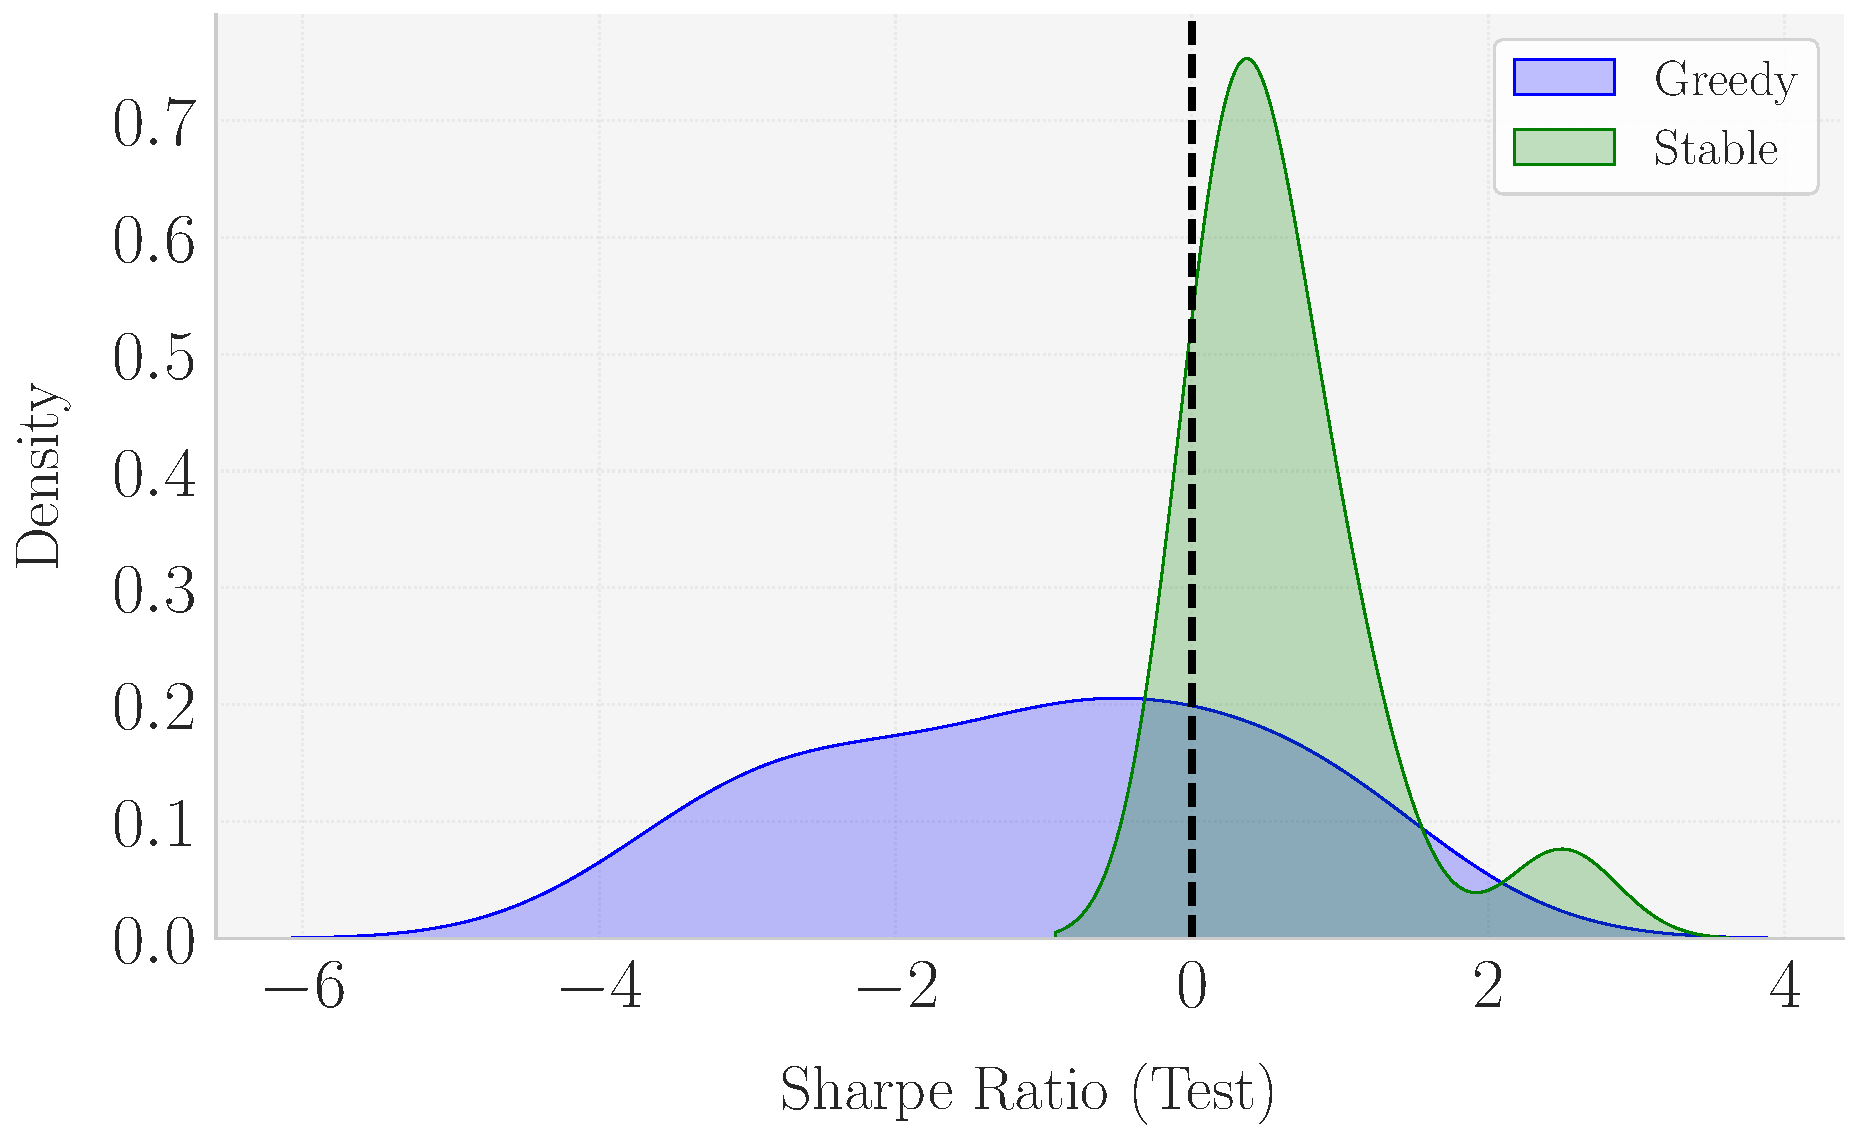
\includegraphics[width=\textwidth]{/Users/jesusvillotamiranda/Library/CloudStorage/OneDrive-UniversidaddeLaRioja/CEMFI/__MSc__/__Second_year__/6th_Term/MasterThesis/__Output/KMeans_RobustnessCheck_SR_Test_Set_Distribution_[Change_theta].pdf}
    \caption{\textbf{KMeans}: Distribution of $SR^{\mathcal P^{test}}(\theta)$}
    \label{fig:KMeans_Robustness_theta_Distr}
  \end{subfigure}
  \hspace{0.05\textwidth} % Add horizontal space between the subfigures
  \begin{subfigure}[b]{0.46\textwidth}
    \centering
    \includegraphics[width=\textwidth]{/Users/jesusvillotamiranda/Library/CloudStorage/OneDrive-UniversidaddeLaRioja/CEMFI/__MSc__/__Second_year__/6th_Term/MasterThesis/__Output/KMeans_RobustnessCheck_SR_Test_Set_vs_theta_[Change_theta].pdf}
    \caption{\textbf{KMeans}: Series of $SR^{\mathcal P^{test}}(\theta)$}
    \label{fig:KMeans_Robustness_theta_Series}
  \end{subfigure}
  
  \bx 
      \begin{subfigure}[b]{0.46\textwidth}
    \centering
    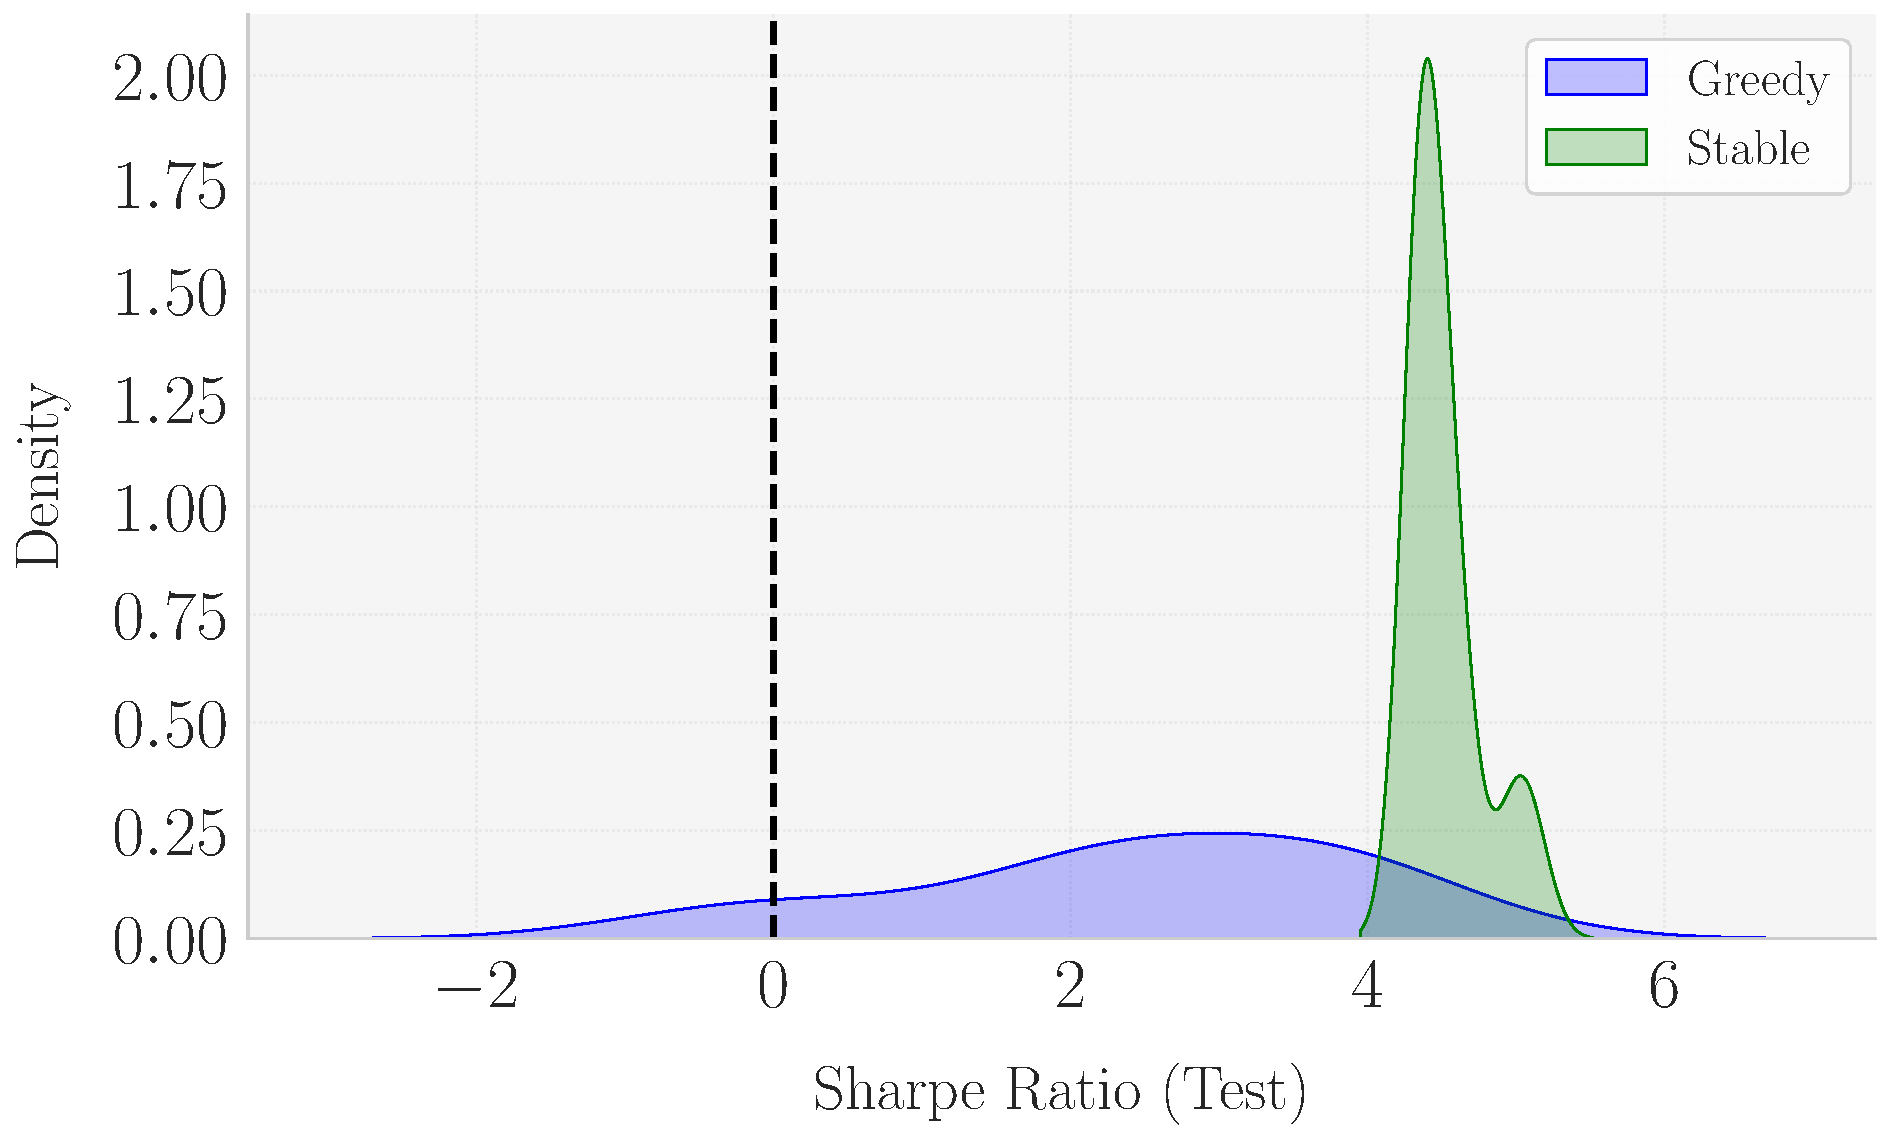
\includegraphics[width=\textwidth]{/Users/jesusvillotamiranda/Library/CloudStorage/OneDrive-UniversidaddeLaRioja/CEMFI/__MSc__/__Second_year__/6th_Term/MasterThesis/__Output/LLAMA_RobustnessCheck_SR_Test_Set_Distribution_[Change_theta].pdf}
    \caption{\textbf{LLM}: Distribution of $SR^{\mathcal P^{test}}(\theta)$}
    \label{fig:LLM_Robustness_theta_Distr}
  \end{subfigure}
  \hspace{0.05\textwidth} % Add horizontal space between the subfigures
  \begin{subfigure}[b]{0.46\textwidth}
    \centering
    \includegraphics[width=\textwidth]{/Users/jesusvillotamiranda/Library/CloudStorage/OneDrive-UniversidaddeLaRioja/CEMFI/__MSc__/__Second_year__/6th_Term/MasterThesis/__Output/LLAMA_RobustnessCheck_SR_Test_Set_vs_theta_[Change_theta].pdf}
    \caption{\textbf{LLM}: Series of $SR^{\mathcal P^{test}}(\theta)$}
    \label{fig:LLM_Robustness_theta_Series}
  \end{subfigure}

\mx 
\subcaption*{\textit{Note: This figure displays the sensitivity of the Sharpe Ratios ($SR^{\mathcal P^{test}}$) to variations in the upper bound on the number of traded clusters ($\theta$), with $L$ fixed at 4. Panels \textsc{(a)} and \textsc{(b)} show the distribution and series of $SR^{\mathcal P^{test}}(\theta)$ for KMeans clustering, respectively, while Panels \textsc{(c)} and \textsc{(d)} illustrate the same for LLM-based clustering. For KMeans, the results are mixed: the \textit{Stable} algorithm generates positive Sharpe Ratios for low $\theta$ values, whereas the \textit{Greedy} algorithm performs better with high $\theta$ values, indicating sensitivity and instability. In contrast, the LLM-based clustering shows a more consistent pattern, with a concentration of positive Sharpe Ratios across a broader range of $\theta$ values, suggesting greater robustness and stability in the trading strategy.}}

\label{fig:Robustness_theta}
\end{figure}
%----------------------------------------------------


The results of this exercise are shown in \cref{fig:Robustness_theta}. As we can see, in \cref{fig:KMeans_Robustness_theta_Distr} the results are mixed for the case of KMeans clustering. Namely, the \textit{Stable} algorithm is able to generate positive Sharpe Ratios but the \textit{Greedy} algorithm struggles to do so. In \cref{fig:KMeans_Robustness_theta_Series} we see what is happening: \textit{Stable} works well with for low values of $\theta$, while \textit{Greedy} only works for high values of $\theta$. This high reliance of the algorithms on specific values of $\theta$ points to the instability of the trading strategy when employing KMeans clustering.

\mx 
On the other hand, \cref{fig:LLM_Robustness_theta_Distr} shows a clear pattern for the case of LLM clustering. Namely, the mass accumulates at high and positive Sharpe Ratios. This observation is further substantiated by \cref{fig:KMeans_Robustness_theta_Series}, which shows that leaving aside the fact that the greedy algorithm does bad for really low values of $\theta$ (i.e.: $\theta\leq 3$), in general, the trading strategy is now able to produce high, positive and stable Sharpe Ratios across different values of $\theta$.  

\mx
All in all, our results are robust to hyperparameter variability, showing that LLM clustering consistently beats a strategy based on clustering embeddings with KMeans. 


%%%%%%%%%%%%%%%%% CONCLUSION %%%%%%%%%%%%%%%%%%%%%%
%----------------------------------------------------
\section{Conclusion}
%----------------------------------------------------
%\hspace{0.5cm} 
This paper investigates how information from business news affects stock market prices. We analyze a dataset of Spanish business articles during a particularly volatile period-the COVID-19 pandemic-and examine firm-specific stock market reactions to news. We show that transforming text into vector embeddings and clustering them using KMeans yields clusters that are firm-specific and industry-specific. However, the distribution of articles across clusters is unstable over sequential data splits, indicating temporal instability. When we implement a cluster-based trading strategy-similar to portfolio sorts-on the KMeans clusters, we observe an over-reliance on the past performance of a cluster. That is, signals are short-lived due to temporal instability. Consequently, the out-of-sample profitability of the trading strategy is negligible, evidencing the method's poor temporal generalizability. Therefore, a model based on embeddings is superficial and is not able to anticipate market trends.

%----------------------------------------------------
Alternatively, we develop a novel approach by guiding a Large Language Model (LLM) through a structured news-parsing schema, enabling it to analyze news-implied firm-specific economic shocks. The schema involves identifying the firms affected by the articles and classifying the implied shocks on such firms by their type, magnitude, and direction. This LLM-based methodology demonstrates several advantages over the traditional clustering approach. Even in a volatile period, it produces stable distributions of articles across clusters in sequential splits, demonstrating robust temporal stability. Moreover, the resulting trading signals are both long-lasting and economically relevant, as they are based on fundamental economic shocks rather than statistical patterns. The results show that the LLM-based trading strategy effectively identifies winners and losers, illustrating the parser's ability to anticipate market trends by comprehending the economic implications of firm-specific shocks. This approach generates a consistent profile of earnings in the test set, with results robust to the choice of hyperparameters-the holding period length of the trading strategy and the number of selected clusters for trading. Our findings demonstrate a promising avenue: LLMs, when guided by appropriate economic frameworks, can help predict market reactions to news through systematic classification of economic shocks embedded in financial narratives.


%%%%%%%%%%%%%%%%%% BIBLIOGRAPHY %%%%%%%%%%%%%%%%%%%%%%
\bibliography{bib_references.bib}
\bibliographystyle{plain}

%----------------------------------------------------
\newpage
% To make sure all the tables/figures appear before the appendix
\processdelayedfloats 
% Reset the numbering for appendix figures and tables
\renewcommand{\thefigure}{A\arabic{figure}} 
\renewcommand{\thetable}{A\arabic{table}}
%----------------------------------------------------

%%%%%%%%%%%%%%%%%% APPENDIX %%%%%%%%%%%%%%%%%%%%%%
\appendix
\section{Appendix}
\subsection{KMeans Algorithm}
%----------------------------------------------------
% Alternative 1: Algorithmic Setup
\begin{algorithm}[H]
\caption{KMeans Clustering Algorithm}
\label{alg:KMeans}
\begin{algorithmic}[1]
\State \textbf{Input:} Embedding vectors $\{\mathbf{e}^1, \mathbf{e}^2, \ldots, \mathbf{e}^{N}\}$, number of clusters $k$
\State \textbf{Output:} Cluster assignments $\{\D_1, \D_2, \ldots, \D_k\}$, centroids $\{\mathbf{c}_1, \mathbf{c}_2, \ldots, \mathbf{c}_k\}$

\State \textbf{Initialize} centroids $\{\mathbf{c}_1, \mathbf{c}_2, \ldots, \mathbf{c}_k\}$ randomly

\Repeat
    \State \underline{\textit{Assignment Step:}}
    \For{each vector $\mathbf{e}^i$}
        \State Assign $\mathbf{e}^i$ to the nearest centroid:
        \[
        g = \arg \min_{\ell\in\{1,...,k\}} \|\mathbf{e}^i - \mathbf{c}_{\ell}\|_{2}^2
        \]
        \State Update cluster assignments: $\D_{g} \leftarrow \D_{g} \cup \{i\}$
    \EndFor

    \State \underline{\textit{Update Step:}}
    \For{each cluster $\D_g$}
        \State Recalculate centroid $\mathbf{c}_g$:
        \[
        \mathbf{c}_g = \frac{1}{|\D_g|} \sum_{i \in \D_g} \mathbf{e}^i
        \]
    \EndFor
\Until{cluster assignments no longer change}

\State \textbf{Return} cluster assignments $\{\D_1, \D_2, \ldots, \D_k\}$ and centroids $\{\mathbf{c}_1, \mathbf{c}_2, \ldots, \mathbf{c}_k\}$

\end{algorithmic}
\end{algorithm}

%----------------------------------------------------
% Alternative 2: More organized setup
%\section*{KMeans Clustering Algorithm}

\subsection*{Inputs}
\begin{itemize}
    \item Embedding vectors: $\{\mathbf{e}^1, \mathbf{e}^2, \ldots, \mathbf{e}^{N_{tr}}\}$
    \item Number of clusters: $k$
\end{itemize}

\subsection*{Outputs}
\begin{itemize}
    \item Cluster assignments: $\{C_1, C_2, \ldots, C_k\}$
    \item Centroids: $\{\mathbf{c}_1, \mathbf{c}_2, \ldots, \mathbf{c}_k\}$
\end{itemize}

\subsection*{Algorithm}
\begin{enumerate}
    \item \textbf{Initialize} centroids $\{\mathbf{c}_1, \mathbf{c}_2, \ldots, \mathbf{c}_k\}$ randomly.
    \item \textbf{Repeat until convergence:}
    \begin{enumerate}
        \item \textbf{Assignment Step:}
        \[
        C_j = \left\{ \mathbf{e}^i \mid j = \arg \min_{l} \|\mathbf{e}^i - \mathbf{c}_l\|^2, \quad l = 1, 2, \ldots, k \right\}
        \]
        \item \textbf{Update Step:}
        \[
        \mathbf{c}_j = \frac{1}{|C_j|} \sum_{\mathbf{e}^i \in C_j} \mathbf{e}^i, \quad \forall j = 1, 2, \ldots, k
        \]
    \end{enumerate}
    \item \textbf{Convergence Criterion:} Repeat steps 2(a) and 2(b) until the cluster assignments do not change, i.e.,
    \[
    C_j^{(t+1)} = C_j^{(t)}, \quad \forall j = 1, 2, \ldots, k
    \]
    where $t$ denotes the iteration number.
\end{enumerate}

\subsection*{Objective}
The KMeans algorithm aims to minimize the within-cluster sum of squares (WCSS):
\[
\min_{C, \mathbf{c}} \sum_{j=1}^k \sum_{\mathbf{e}^i \in C_j} \|\mathbf{e}^i - \mathbf{c}_j\|^2
\]


%----------------------------------------------------

\newpage
%%%%%%%%%%%%%%%%%%%%%%%%%%%%%%%%%%%%%%%%%%%%%%%%%%%%%
\subsection{Hyperparameter Choice}
Our hyperparameters are $L$ and $\theta$. Recall that $L$ denotes the number of trading days over which we hold the positions in the beta-neutral strategy, while $\theta$ represents the upper bound on each side (long and short) for the amount of clusters we select for the trading strategy. The specific choice of hyperparameters we made for the results presented in the paper were:
\begin{align*}
L &= 4
\\
\theta &= \integer{0.5k}
\end{align*}
where $k$ represents the number of clusters (26 for KMeans clustering, and 20 for LLM clustering). This choice is not arbitrary nor opportunistic. Instead, it results from the maximization of the Sharpe Ratio of the portfolio in the train and validation samples for both KMeans and LLM clustering. This choice procedure is completely based on \textit{in-sample} criteria and it prevents lookahead bias. The justification for such choices is made below.

\subsubsection{KMeans Clustering}

In \cref{fig:KMeans_hyperparameter_justification_L} we can see that a choice of $L=4$ in the training and validation splits generates the most stable Sharpe Ratio. Namely, In the train set (\cref{fig:K_hyp_1}), it makes more sense to choose low values of $L$ (less than 4) to maximize the $SR$. However, in the validation set (\cref{fig:K_hyp_2}), it makes more sense to choose higher values of $L$. The choice of $L=4$ represents a balanced compromise, providing a stable Sharpe Ratio profile across both splits, ensuring consistent in-sample performance.
%The choice of $L=4$ stands as a middle ground between this contradiction, generating a stable choice and a stable profile of earnings in sample.

%----------------------------------------------------
\inserthere{fig:KMeans_hyperparameter_justification_L}
\begin{figure}[H]
  \caption{Sharpe Ratios in the train and validation splits as a function of $L$ (KMeans)}
  \centering
  
  \begin{subfigure}[b]{0.46\textwidth}
    \centering
    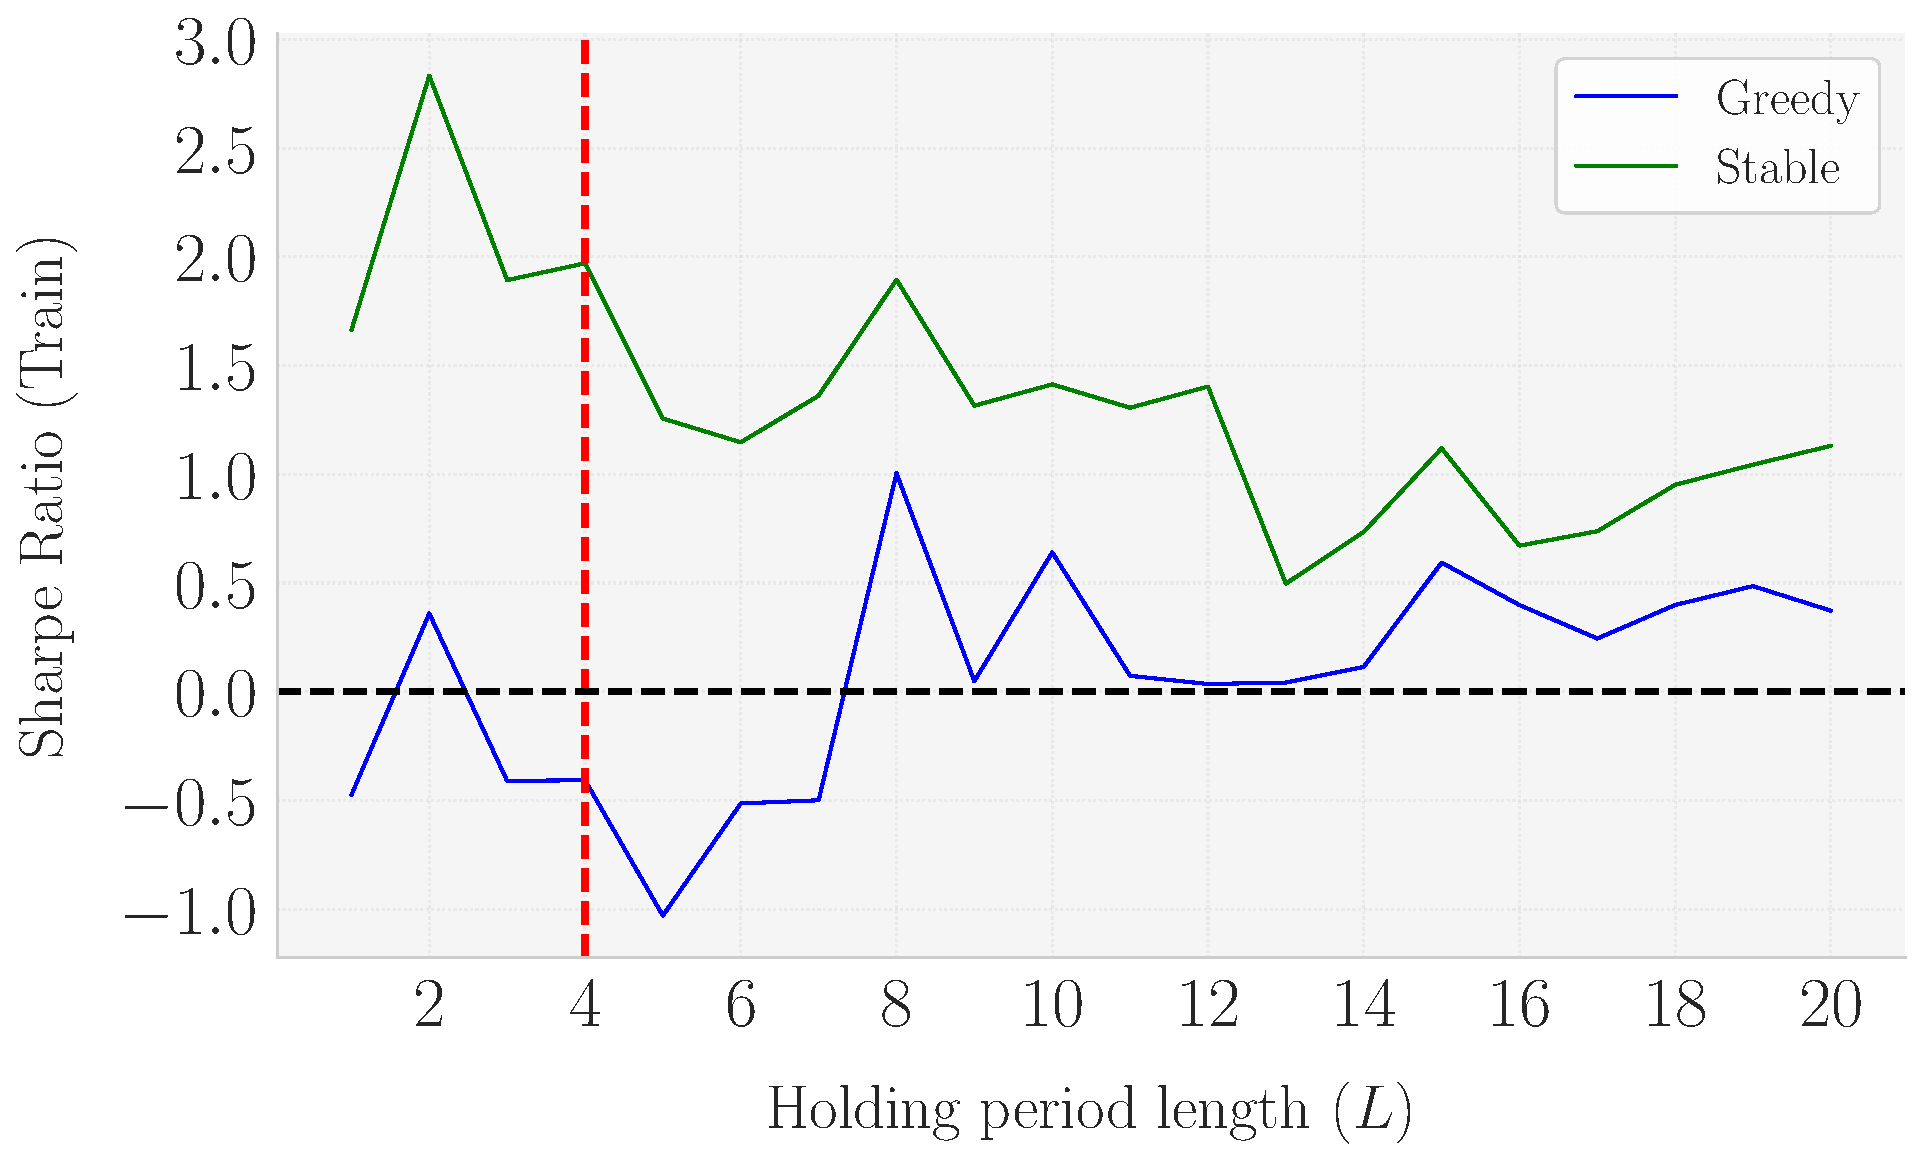
\includegraphics[width=\textwidth]{/Users/jesusvillotamiranda/Library/CloudStorage/OneDrive-UniversidaddeLaRioja/CEMFI/__MSc__/__Second_year__/6th_Term/MasterThesis/__Output/KMeans_RobustnessCheck_SR_Train_Set_vs_L_[Change_L].pdf}
    \caption{Plot of $SR^{\mathcal P^{tr}}(L)$ over a grid of $L$}
    \label{fig:K_hyp_1}
  \end{subfigure}
  \hspace{0.05\textwidth} % Add horizontal space between the subfigures
  \begin{subfigure}[b]{0.46\textwidth}
    \centering
    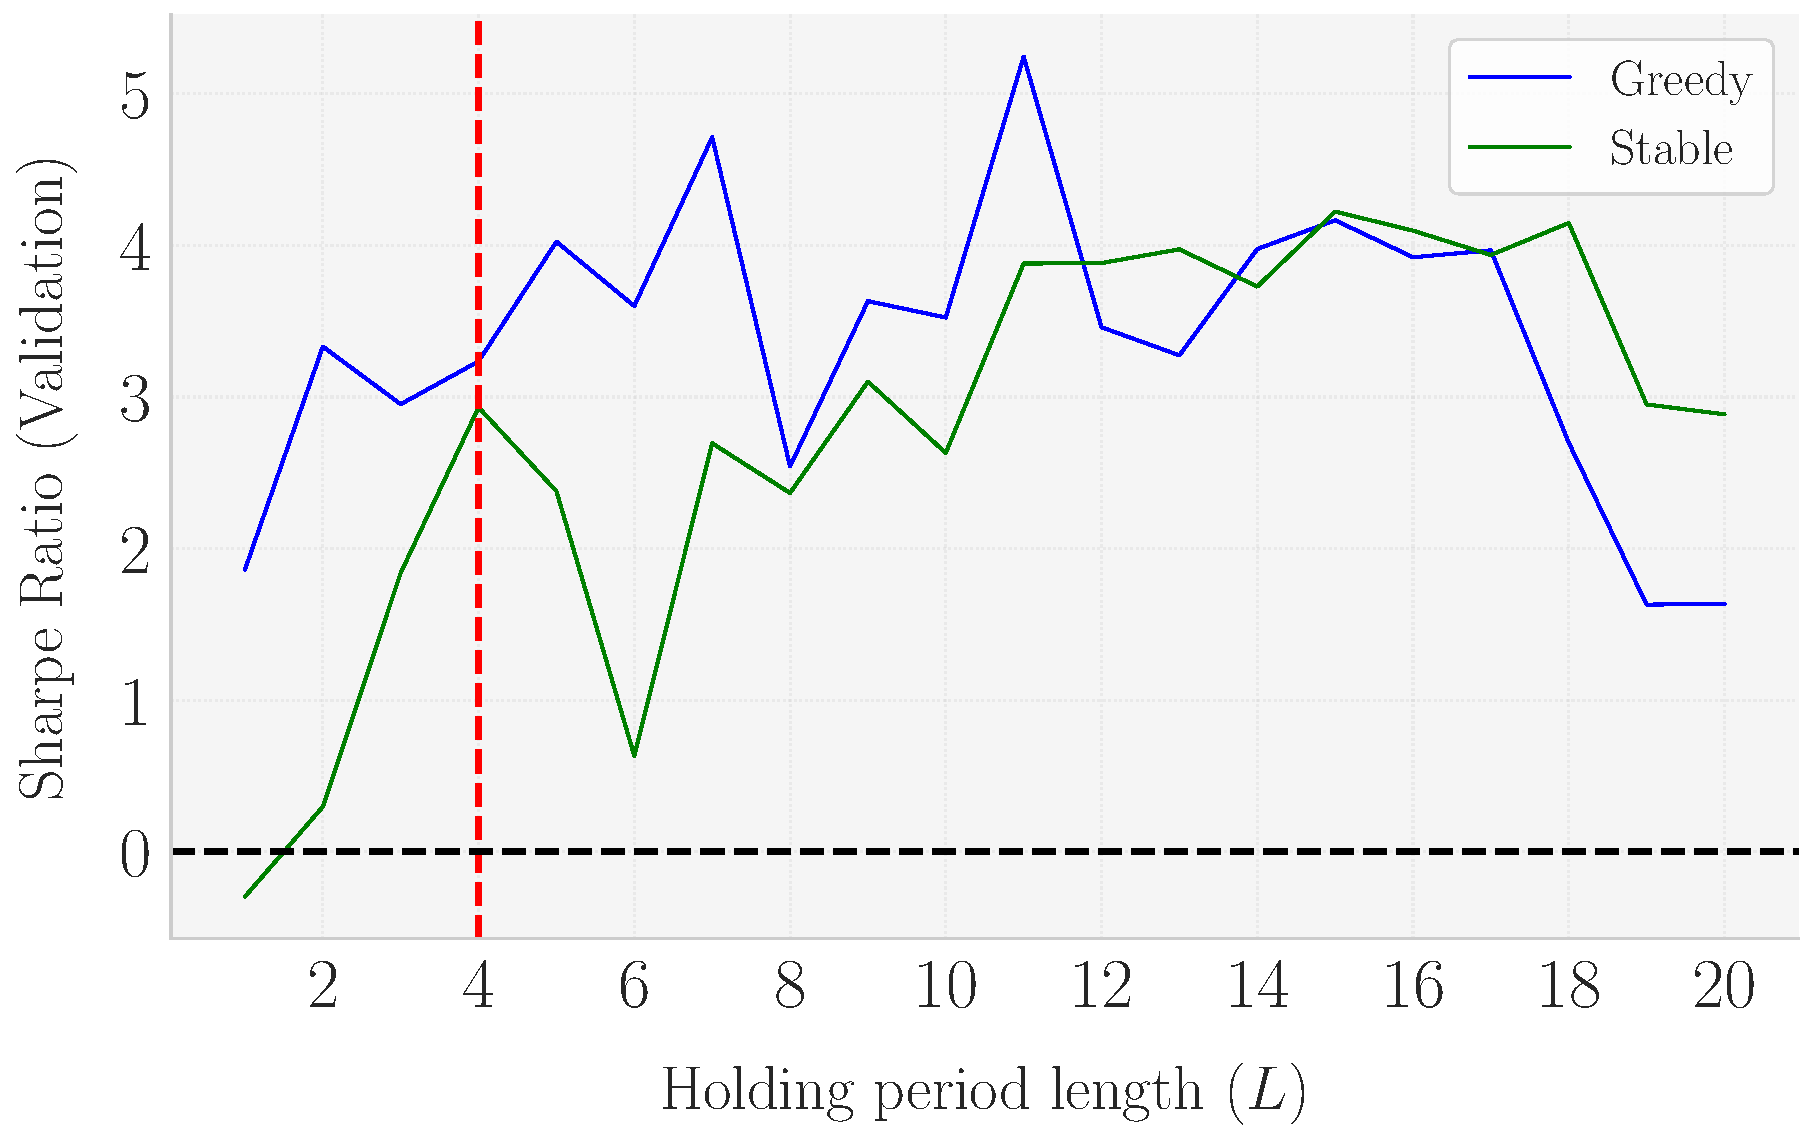
\includegraphics[width=\textwidth]{/Users/jesusvillotamiranda/Library/CloudStorage/OneDrive-UniversidaddeLaRioja/CEMFI/__MSc__/__Second_year__/6th_Term/MasterThesis/__Output/KMeans_RobustnessCheck_SR_Validation_Set_vs_L_[Change_L].pdf}
    \caption{Plot of $SR^{\mathcal P^{val}}(L)$ over a grid of $L$}
    \label{fig:K_hyp_2}
  \end{subfigure}  
  \mx
  \subcaption*{\textit{Note: This figure shows the Sharpe Ratios ($SR$) as a function of the holding period length ($L$) for the KMeans clustering method in the training (Panel a) and validation (Panel b) splits. In Panel (a), the Sharpe Ratios in the training set indicate that lower values of $L$ (less than 4) maximize performance. Conversely, in Panel (b), the validation set shows higher Sharpe Ratios for longer holding periods. The choice of $L=4$ represents a balanced compromise, providing a stable Sharpe Ratio profile across both splits, ensuring consistent in-sample performance without introducing lookahead bias.}}
  \label{fig:KMeans_hyperparameter_justification_L}
\end{figure}
%----------------------------------------------------

On the other hand, the choice of $\theta=\integer{0.5\cd 26}=13$ is a choice that pursues stability in the Sharpe Ratio of the train and validation portfolios. As we can see from \cref{fig:KMeans_hyperparameter_justification_theta}, the Sharpe Ratios tend to converge to the highest and most stable value when we choose the highest possible value of $\theta$. 

 %----------------------------------------------------
\inserthere{fig:KMeans_hyperparameter_justification_theta}
\begin{figure}[H]
  \caption{Sharpe Ratios in the train and validation splits as a function of $\theta$ (KMeans)}
  \centering
    \begin{subfigure}[b]{0.46\textwidth}
    \centering
    \includegraphics[width=\textwidth]{/Users/jesusvillotamiranda/Library/CloudStorage/OneDrive-UniversidaddeLaRioja/CEMFI/__MSc__/__Second_year__/6th_Term/MasterThesis/__Output/KMeans_RobustnessCheck_SR_Train_Set_vs_theta_[Change_theta].pdf}
    \caption{Plot of $SR^{\mathcal P^{tr}}(\theta)$ over a grid of $\theta$}
    \label{fig:K_hyp_3}
  \end{subfigure}
  \hspace{0.05\textwidth} % Add horizontal space between the subfigures
  \begin{subfigure}[b]{0.46\textwidth}
    \centering
    \includegraphics[width=\textwidth]{/Users/jesusvillotamiranda/Library/CloudStorage/OneDrive-UniversidaddeLaRioja/CEMFI/__MSc__/__Second_year__/6th_Term/MasterThesis/__Output/KMeans_RobustnessCheck_SR_Validation_Set_vs_theta_[Change_theta].pdf}
    \caption{Plot of $SR^{\mathcal P^{val}}(\theta)$ over a grid of $\theta$}
    \label{fig:K_hyp_4}
  \end{subfigure}
  \mx
\subcaption*{\textit{Note: This figure illustrates the Sharpe Ratios ($SR$) as a function of $\theta$, the upper bound on the number of traded clusters, for the KMeans clustering method in the training (Panel a) and validation (Panel b) splits. In Panel (a), the Sharpe Ratios in the training set show a trend of increasing stability and maximizing performance as $\theta$ approaches its upper limit. Similarly, Panel (b) displays a consistent pattern in the validation set, where higher values of $\theta$ lead to convergence at the highest and most stable Sharpe Ratios. The choice of $\theta = 13$ (i.e: $\integer{0.5 \cdot 26}$) reflects this observed stability and optimization, providing a balanced and robust selection for the portfolio strategy.}}
  \label{fig:KMeans_hyperparameter_justification_theta}
\end{figure}
%----------------------------------------------------


\subsubsection{LLM Clustering}
Following a similar logic as below, the choice of $L=4$ sets a consensus between the maximization of $SR^{\mathcal P^{tr}}$ and $SR^{\mathcal P^{val}}$. That is, maximizing $SR^{\mathcal P^{tr}}$ requires lower holding period lengths (the maximizer is $L=4$), while maximizing $SR^{\mathcal P^{val}}$ requires increasing the window length. Among this contradiction, $L=4$ standing as a perfect choice to balance the maximization requirements in both samples, generating a stable choice for the holding period window length.

%----------------------------------------------------
\inserthere{fig:LLM_hyperparameter_justification_L}
\begin{figure}[H]
  \caption{Sharpe Ratios in the train and validation splits as a function of hyperparameters (LLM)}
  \centering
  
  \begin{subfigure}[b]{0.46\textwidth}
    \centering
    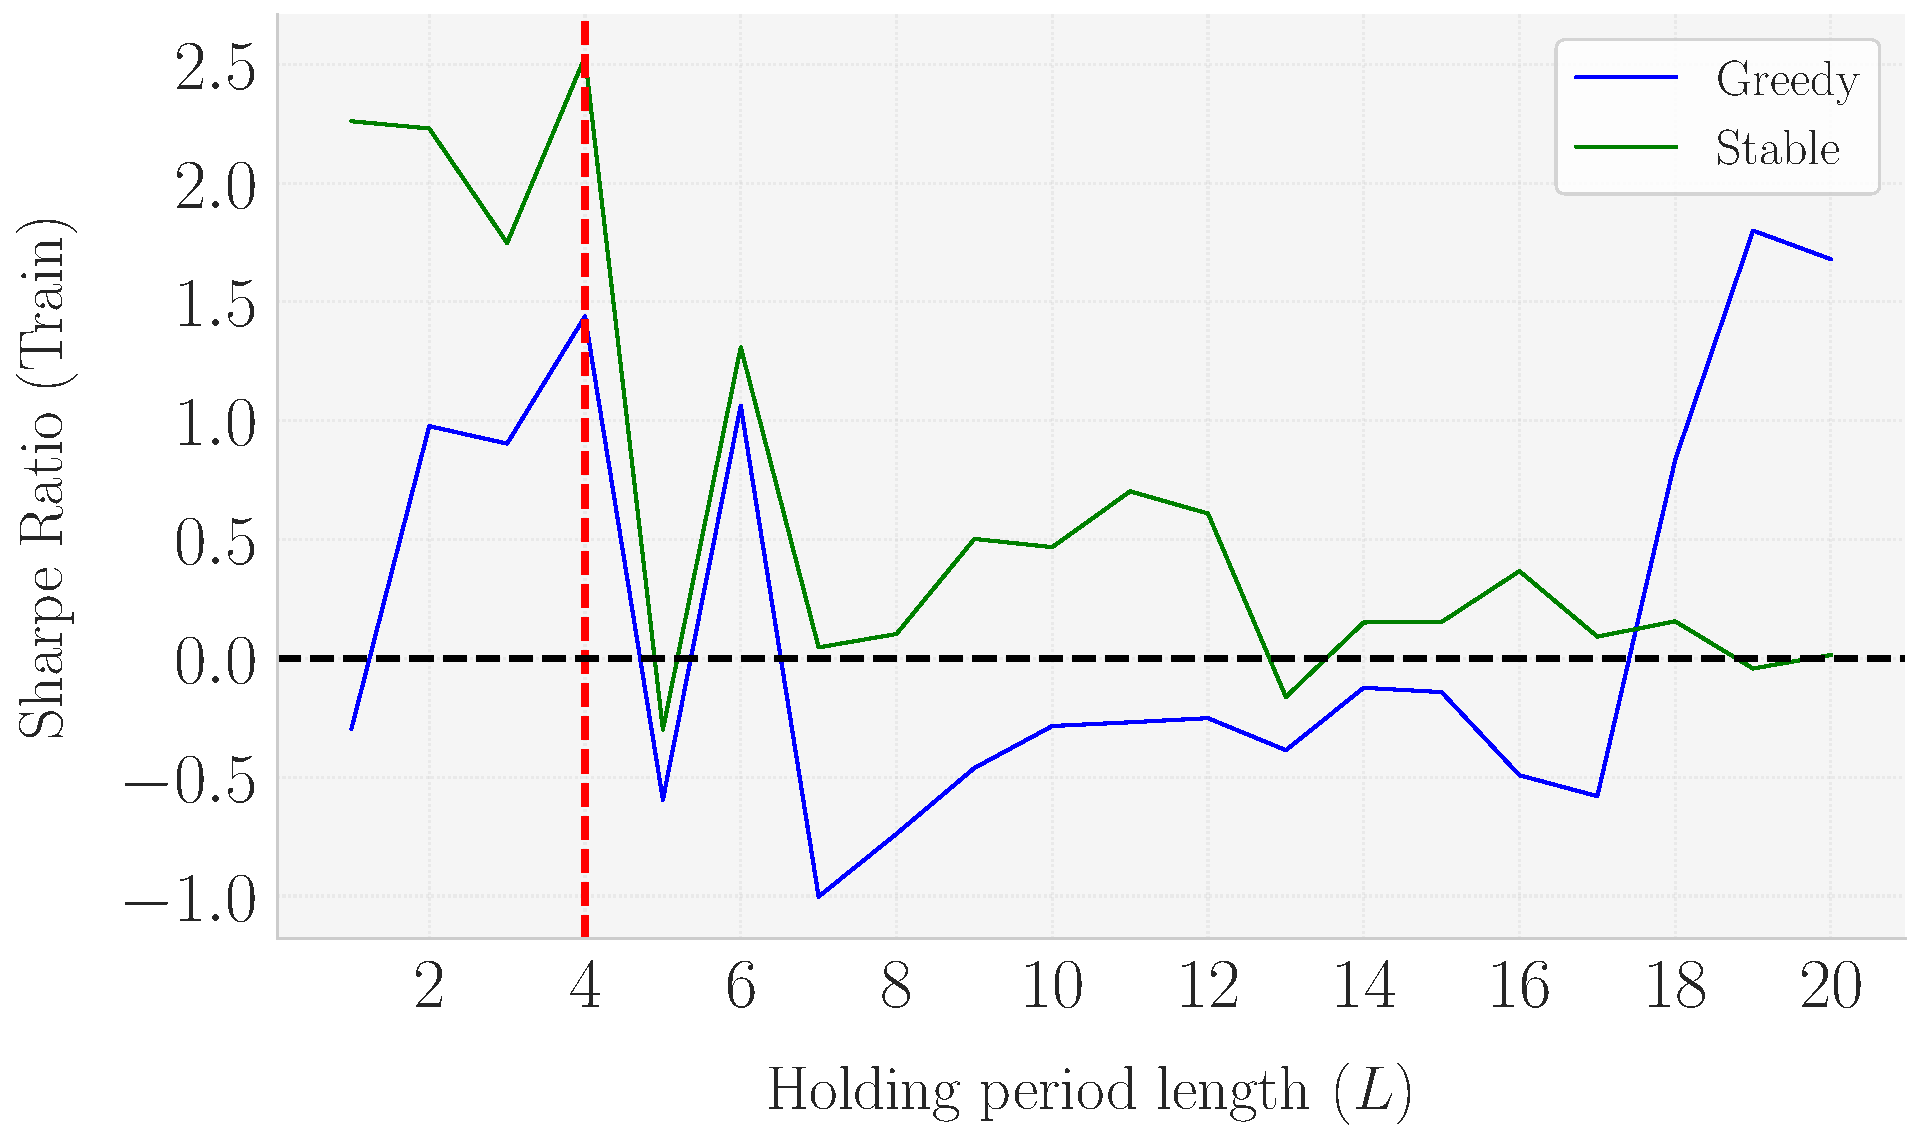
\includegraphics[width=\textwidth]{/Users/jesusvillotamiranda/Library/CloudStorage/OneDrive-UniversidaddeLaRioja/CEMFI/__MSc__/__Second_year__/6th_Term/MasterThesis/__Output/LLAMA_RobustnessCheck_SR_Train_Set_vs_L_[Change_L].pdf}
    \caption{Plot of $SR^{\mathcal P^{tr}}(L)$ over a grid of $L$}
    \label{fig:LLM_hyp_1}
    
  \end{subfigure}
  \hspace{0.05\textwidth} % Add horizontal space between the subfigures
  \begin{subfigure}[b]{0.46\textwidth}
    \centering
    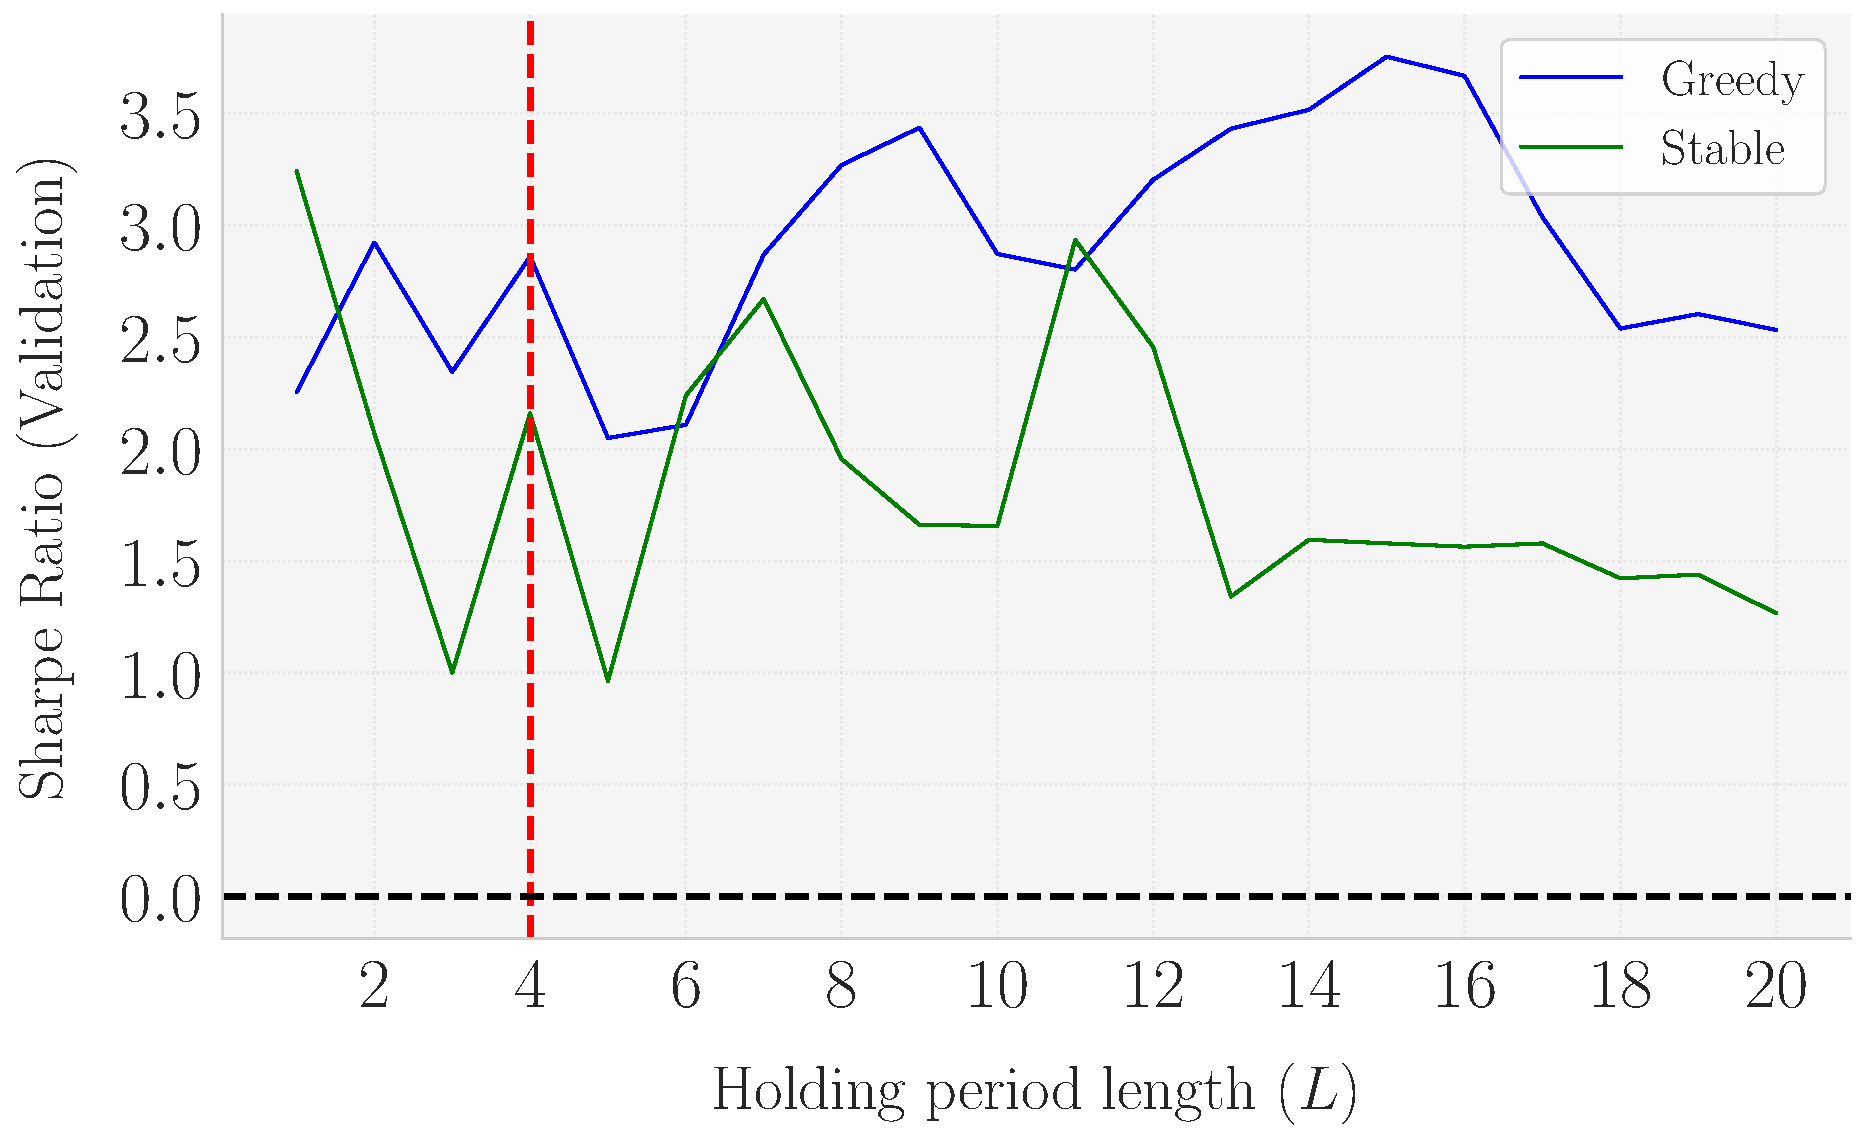
\includegraphics[width=\textwidth]{/Users/jesusvillotamiranda/Library/CloudStorage/OneDrive-UniversidaddeLaRioja/CEMFI/__MSc__/__Second_year__/6th_Term/MasterThesis/__Output/LLAMA_RobustnessCheck_SR_Validation_Set_vs_L_[Change_L].pdf}
    \caption{Plot of $SR^{\mathcal P^{val}}(L)$ over a grid of $L$}
    \label{fig:LLM_hyp_2}
  \end{subfigure}
  \mx 
  \subcaption*{\textit{Note: This figure shows the Sharpe Ratios ($SR$) as a function of the holding period length ($L$) for the LLM clustering method, across the training (Panel a) and validation (Panel b) splits. In Panel (a), the Sharpe Ratios in the training set reach their maximum at $L=4$, suggesting shorter holding periods are more effective for maximizing performance. Conversely, Panel (b) illustrates that longer holding periods yield higher Sharpe Ratios in the validation set. The choice of $L=4$ serves as a compromise, balancing the trade-off between maximizing $SR$ in both splits and providing a stable and consistent holding period length for the strategy.}}
  \label{fig:LLM_hyperparameter_justification_L}
\end{figure}
%----------------------------------------------------

Finally, the same conclusion as in KMeans applies here. By selecting $\theta=\integer{0.5\cd 20}=10$, we get a stable Sharpe Ratio. Even though we observe that $SR^{\mathcal P^{tr}}(L)$ falls momentarily at $\theta=10$ for the Greedy algorithm, it still constitutes a good choice. Conversely, at $\theta=10$ the greedy algorithm sees a jump in $SR^{\mathcal P^{val}}(L)$. All in all, we can easily conclude that $\theta=\integer{0.5k}$ arises as a good hyperpamrameter choice also for LLM clustering.
%----------------------------------------------------
\inserthere{fig:LLM_hyperparameter_justification_theta}
\begin{figure}[H]
\caption{Sharpe Ratios in the train and validation splits as a function of $\theta$ (LLM)}
  \centering

    \begin{subfigure}[b]{0.46\textwidth}
    \centering
    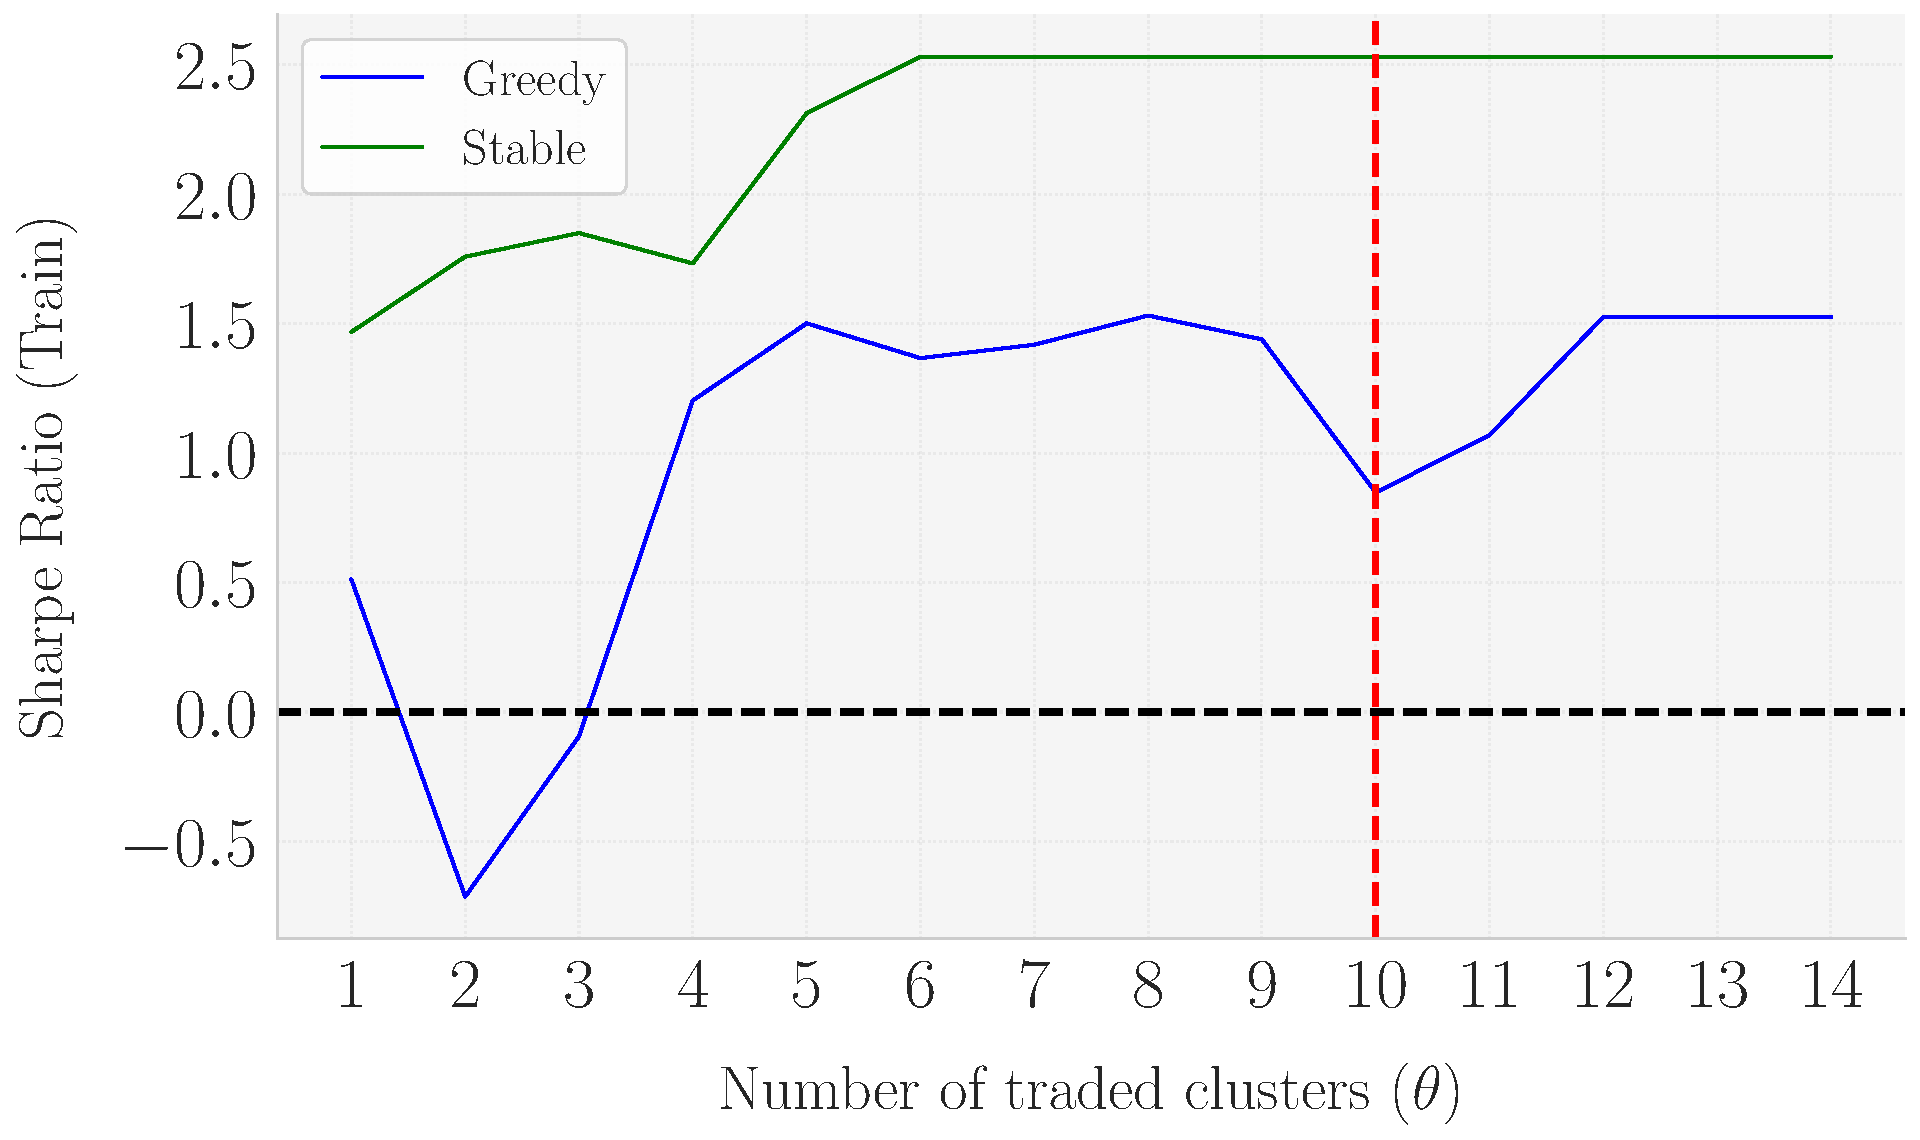
\includegraphics[width=\textwidth]{/Users/jesusvillotamiranda/Library/CloudStorage/OneDrive-UniversidaddeLaRioja/CEMFI/__MSc__/__Second_year__/6th_Term/MasterThesis/__Output/LLAMA_RobustnessCheck_SR_Train_Set_vs_Theta_[Change_theta].pdf}
    \caption{Plot of $SR^{\mathcal P^{tr}}(\theta)$ over a grid of $\theta$}
    \label{fig:LLM_hyp_3}
  \end{subfigure}
  \hspace{0.05\textwidth} % Add horizontal space between the subfigures
  \begin{subfigure}[b]{0.46\textwidth}
    \centering
    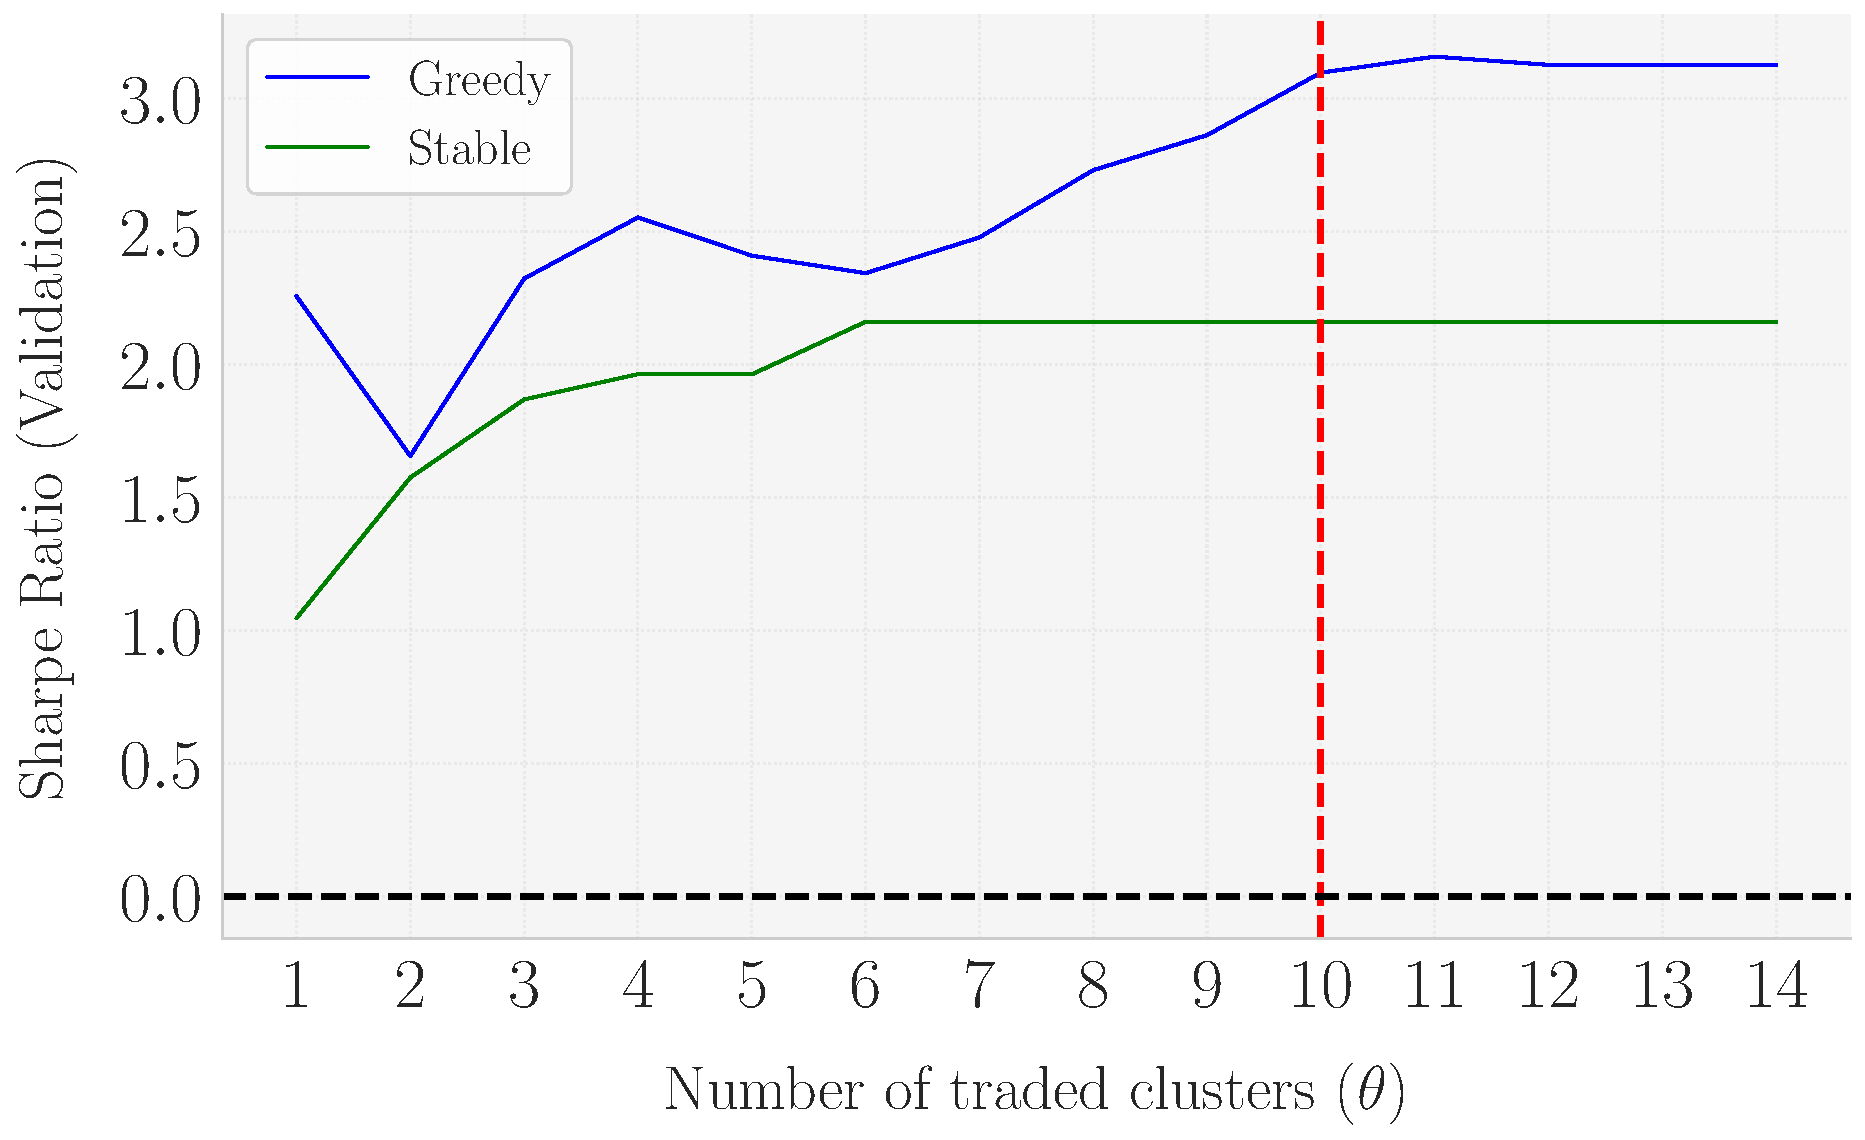
\includegraphics[width=\textwidth]{/Users/jesusvillotamiranda/Library/CloudStorage/OneDrive-UniversidaddeLaRioja/CEMFI/__MSc__/__Second_year__/6th_Term/MasterThesis/__Output/LLAMA_RobustnessCheck_SR_Validation_Set_vs_Theta_[Change_theta].pdf}
    \caption{Plot of $SR^{\mathcal P^{val}}(\theta)$ over a grid of $\theta$}
    \label{fig:LLM_hyp_4}
  \end{subfigure}
\mx
\subcaption*{\textit{Note: This figure illustrates the Sharpe Ratios ($SR$) as a function of $\theta$, the upper bound on the number of traded clusters, for the LLM clustering method in the training (Panel a) and validation (Panel b) splits. In Panel (a), the Sharpe Ratios for the training set indicate a temporary dip at $\theta=10$ for the Greedy algorithm, yet this value still provides a relatively stable outcome. In contrast, Panel (b) shows that $\theta=10$ leads to a noticeable increase in Sharpe Ratios for the validation set, particularly benefiting the Greedy algorithm. The choice of $\theta = \integer{0.5k} = 10$ strikes a balance, confirming it as an effective hyperparameter selection for achieving stability in both the training and validation splits with LLM clustering.}}
\label{fig:LLM_hyperparameter_justification_theta}
\end{figure}
%----------------------------------------------------


%%%%%%%%%%%%%%%%%%%%%%%%%%%%%%%%%%%%%%%%%%%%%%%%%%%%%

\newpage
%%%%%%%%%%%%%%%%%%%%%%%%%%%%%%%%%%%%%%%%%%%%%%%%%%%%%
\subsection{Optimal Cluster Selection Algorithms}
%%%%%%%%%%%%%%%%%%%%%%%%%%%%%%%%%%%%%%%%%%%%%%%%%%%%%
%----------------------------------------------------
\begin{algorithm}
\caption{
\textsc{Greedy Selection} 
~|~
{{Top average Sharpe Ratio in Validation Set}}
}
%%%%%%%%%%%%%%%%%%%%%%%%%%%%%%%%%%%%%%%%%%%%%%%%%%%%%
\label{alg:greedy_selection}
%%%%%%%%%%%%%%%%%%%%%%%%%%%%%%%%%%%%%%%%%%%%%%%%%%%%%
\begin{algorithmic}[1]
\mx 
\State \textbf{Input:} Set of clusters $\mathcal{G} = \{1, 2, \ldots, k^*\}$, Sharpe Ratios in the validation sample $\{SR_L^{(i,j)}\}_{(i,j)\in \mathcal B^{val}}$, maximum number of traded clusters $\theta\in\mathbb{N}$ (usually, $\theta\propto k^*)$

\mx 
\State \textbf{Output:} Set of long-traded clusters $\mathcal{G}_{\theta}^{+}$ and set of short-traded clusters $\mathcal{G}_{\theta}^{-}$
%----------------------------------------------------
%\Statex
\vspace{0.4cm}
\Statex \underline{\textit{Step \#1: Compute Cluster Average Sharpe Ratios in Validation Set}}
\For{each $g \in \mathcal{G}$}
    \State Compute average Sharpe Ratio ~
$
\overline{S R}_g^{val} \leftarrow \frac{1}{|\mathcal{B}_g^{val} |} \sum_{(i,j) \in \mathcal{B}_g^{val}} S R_{{{L}}}^{(i,j)}
$
\EndFor
%----------------------------------------------------
%\Statex
\vspace{0.4cm}
\Statex \underline{\textit{Step \#2: Identify Positive and Negative Sharpe Ratio Clusters}}
\State Define $\mathcal{G}_{SR^+}^{val} \leftarrow \{ g \in \mathcal{G} \mid \overline{SR}_g^{val} > 0 \}$
\State Define $\mathcal{G}_{SR^-}^{val} \leftarrow \{ g \in \mathcal{G} \mid \overline{SR}_g^{val} < 0 \}$
%----------------------------------------------------
\vspace{0.4cm}
\Statex \underline{\textit{Step \#3: Rank Clusters by Average Sharpe Ratio in the Validation Set}}
\For{each $g \in \mathcal{G}$}
	\State Rank the average Sharpe Ratio~~
$
\mathfrak{R}_g^{val} \leftarrow  \sum_{h \in \mathcal{G}} 
\mathbf{1}\1{
\overline{S R}_h^{val} \geq \overline{S R}_g^{val} 
}
$
\EndFor
%\State Sort clusters in descending order of $\overline{SR}_g^{val}$
%%\State
%$$\overline{SR}_{\varkappa_1}^{val} \geq \overline{SR}_{\varkappa_2}^{val} \geq \ldots \geq \overline{SR}_{\varkappa_{k^*}}^{val}$$
%----------------------------------------------------
%\Statex
\vspace{0.4cm}
\Statex \underline{\textit{Step \#4: Select Top $\theta$ Clusters}}
\State Define $\theta^+ \leftarrow \min(\theta, |\mathcal{G}_{SR^+}^{val}|)$
;~~
$\mathcal{G}_{\theta}^{+} \leftarrow \{ g\in\G \mid 1 \leq \mathfrak{R}_g^{val} \leq \theta^+ \}$
%\State 

\State Define $\theta^- \leftarrow \min(\theta, |\mathcal{G}_{SR^-}^{val}|)$
;~~
%\State 
 $\mathcal{G}_{\theta}^{-} \leftarrow \{ g \in\G \mid k^* - \theta^- < \mathfrak{R}_g^{val} \leq k^* \}$
%----------------------------------------------------
%\Statex
\vspace{0.5cm}
\State \textbf{Return} Long-traded clusters $\mathcal{G}_{\theta}^{+}$, Short-traded clusters $\mathcal{G}_{\theta}^{-}$

\end{algorithmic}
\end{algorithm}


%
%\begin{algorithm}[H]
%\caption{Greedy Selection of Clusters Based on Average Sharpe Ratio}
%%%%%%%%%%%%%%%%%%%%%%%%%%%%%%%%%%%%%%%%%%%%%%%%%%%%%%
%\label{alg:greedy_selection}
%%%%%%%%%%%%%%%%%%%%%%%%%%%%%%%%%%%%%%%%%%%%%%%%%%%%%%
%\begin{algorithmic}[1]
%\State \textbf{Input:} Set of clusters $\mathcal{G} = \{1, 2, \ldots, k^*\}$, Sharpe Ratios in the validation sample $\{SR_L^{(i,j)}\}_{(i,j)\in \mathcal{B}^{val}}$, maximum number of traded clusters $\theta \in \mathbb{N}$ (usually, $\theta \propto k^*$)
%\State \textbf{Output:} Set of long-traded clusters $\mathcal{G}_{\theta}^{+}$ and set of short-traded clusters $\mathcal{G}_{\theta}^{-}$
%
%\Statex
%\Statex \underline{\textit{Step \#1: Compute Cluster Average Sharpe Ratios in Validation Set}}
%\For{each $g \in \mathcal{G}$}
%    \State Compute average Sharpe Ratio ~
%    \[
%    \overline{SR}_g^{val} \leftarrow \frac{1}{|\mathcal{B}_g^{val} |} \sum_{(i,j) \in \mathcal{B}_g^{val}} SR_{L}^{(i,j)}
%    \]
%\EndFor
%
%\Statex
%\Statex \underline{\textit{Step \#2: Identify Positive and Negative Sharpe Ratio Clusters}}
%\State Define $\mathcal{G}_{SR^+}^{val} \leftarrow \{ g \in \mathcal{G} \mid \overline{SR}_g^{val} > 0 \}$
%\State Define $\mathcal{G}_{SR^-}^{val} \leftarrow \{ g \in \mathcal{G} \mid \overline{SR}_g^{val} < 0 \}$
%
%\Statex
%\Statex \underline{\textit{Step \#3: Rank Clusters by Average Sharpe Ratio}}
%\State Sort clusters in descending order of $\overline{SR}_g^{val}$
%%\State
%\[
%\overline{SR}_{\varkappa_1}^{val} \geq \overline{SR}_{\varkappa_2}^{val} \geq \ldots \geq \overline{SR}_{\varkappa_{k^*}}^{val}
%\]
%
%\Statex
%\Statex \underline{\textit{Step \#4: Select Top $\theta$ Clusters}}
%\State Define $\theta^+ \leftarrow \min(\theta, |\mathcal{G}_{SR^+}^{val}|)$
%\State Define $\theta^- \leftarrow \min(\theta, |\mathcal{G}_{SR^-}^{val}|)$
%
%\State Define $\mathcal{G}_{\theta}^{+} \leftarrow \{ \varkappa_{\ell} \in \mathcal{G} \mid 1 \leq \ell \leq \theta^+ \}$
%\State Define $\mathcal{G}_{\theta}^{-} \leftarrow \{ \varkappa_{\ell} \in \mathcal{G} \mid k^* - \theta^- < \ell \leq k^* \}$
%
%\Statex
%\State \textbf{Return} Long-traded clusters $\mathcal{G}_{\theta}^{+}$, Short-traded clusters $\mathcal{G}_{\theta}^{-}$
%
%\end{algorithmic}
%\end{algorithm}

%----------------------------------------------------


%----------------------------------------------------
\begin{algorithm}[H]
\caption{
\textsc{Rank Stability}
~ |~
{{Minimal Rank Difference between Train \& Validation Sets}
}}
%%%%%%%%%%%%%%%%%%%%%%%%%%%%%%%%%%%%%%%%%%%%%%%%%%%%%
\label{alg:rank_stability}
%%%%%%%%%%%%%%%%%%%%%%%%%%%%%%%%%%%%%%%%%%%%%%%%%%%%%
\begin{algorithmic}[1]
\mx 
\State \textbf{Input:} Set of clusters $\mathcal{G} = \{1, 2, \ldots, k^*\}$, Sharpe Ratios in the training and validation sample $\{SR_L^{(i,j)}\}_{(i,j)\in \mathcal B^{tr}}$ and $\{SR_L^{(i,j)}\}_{(i,j)\in \mathcal B^{val}}$, maximum number of traded clusters $\theta$
\mx 
\State \textbf{Output:} Set of long-traded clusters $\mathcal{G}_{\theta}^{+}$ and set of short-traded clusters $\mathcal{G}_{\theta}^{-}$
%----------------------------------------------------
%\Statex
\mx
\Statex \underline{\textit{Step \#1: Compute Cluster Average Sharpe Ratios in Training \& Validation Set}}
\For{each $g \in \mathcal{G}$}
    \State Compute average Sharpe Ratio in $\mathcal B^{tr}:$ ~~
$
\overline{S R}_g^{tr} \leftarrow \frac{1}{|\mathcal{B}_g^{tr} |} \sum_{(i,j) \in \mathcal{B}_g^{tr}} S R_{{{L}}}^{(i,j)}
$
    \State Compute average Sharpe Ratio in $\mathcal B^{val}:$ ~
$
\overline{S R}_g^{val} \leftarrow \frac{1}{|\mathcal{B}_g^{val} |} \sum_{(i,j) \in \mathcal{B}_g^{val}} S R_{{{L}}}^{(i,j)}
$
\EndFor
%----------------------------------------------------
%\Statex
\mx
\Statex \underline{\textit{Step \#2: Rank Clusters}}
%\State \# \textit{Step 1: Rank Clusters}
\For{each $g \in \mathcal{G}$}
    \State Rank the average Sharpe Ratios in $\mathcal B^{tr}:$ ~~
%$\{\overline{S R}_g^{tr}\}_{g\in\G}$ 
$
\mathfrak{R}_g^{tr} \leftarrow  \sum_{h \in \mathcal{G}} 
\mathbf{1}\1{
\overline{S R}_h^{t r} \geq \overline{S R}_g^{t r} 
}
$
    \State Rank the average Sharpe Ratios in $\mathcal B^{val}:$ ~
%$\{\overline{S R}_g^{tr}\}_{g\in\G}$ 
$
\mathfrak{R}_g^{val} \leftarrow  \sum_{h \in \mathcal{G}} 
\mathbf{1}\1{
\overline{S R}_h^{val} \geq \overline{S R}_g^{val} 
}
$
\EndFor
%----------------------------------------------------
%\Statex
\mx
\Statex \underline{\textit{Step \#3: Calculate Rank Differences}}
\For{each $g \in \mathcal{G}$}
    \State Calculate rank difference $\delta_g \leftarrow | \mathfrak R_g^{tr} - \mathfrak R_g^{val} |$
\EndFor
%----------------------------------------------------
%\Statex
\mx
\Statex \underline{\textit{Step \#4: Select Top $\theta$ Clusters with Smallest Rank Differences}}
\For{each $g \in \mathcal{G}$}
\State Rank the rank difference $:~~ \mathfrak{R}(\delta_g) \leftarrow \sum_{h\in\G} \mbf{1} \1{ \delta_g \geq  \delta_h }$
\EndFor
\State Select top $2\theta$ clusters with smallest $\delta_g$: 
$
~~
\mathcal{G}_{\theta} = 
\3{
g\in\G \c 1 \leq \mathfrak{R}(\delta_g) \leq 2\theta 
}
~
$
%----------------------------------------------------
%\Statex
\mx
\Statex \underline{\# \textit{Step 5: Determine Long and Short Positions}}
\State Define $\mathcal{G}_{\theta}^{+} = \{g \in \mathcal{G}_{\theta} \mid \overline{SR}_g^{tr} > 0 \text{ and } \overline{SR}_g^{val} > 0\}$
\State Define $\mathcal{G}_{\theta}^{-} = \{g \in \mathcal{G}_{\theta} \mid \overline{SR}_g^{tr} < 0 \text{ and } \overline{SR}_g^{val} < 0\}$
%----------------------------------------------------
%\Statex
\mx
\State \textbf{Return} Long-traded clusters $\mathcal{G}_{\theta}^{+}$, Short-traded clusters $\mathcal{G}_{\theta}^{-}$

\end{algorithmic}
\end{algorithm}


%----------------------------------------------------




%%%%%%%%%%%%%%%%%%%%%%%%%%%%%%%%%%%%%%%%%%%%%%%%%%%%%
\subsection{Sample of articles for each cluster}
%%%%%%%%%%%%%%%%%%%%%%%%%%%%%%%%%%%%%%%%%%%%%%%%%%%%%
\setcounter{table}{0}
\renewcommand{\thetable}{A\arabic{table}} % To ensure the tables in the appendix are numbered as A1, A2, etc.

%%----------------------------------------------------
%%%%%%%%%%%%%%%%%%%%%%%%%%%%%%%%%%%%%%%%%%%%%%%%%%%%%
%%%%%%%%%%%%%% 		ENGLISH 		%%%%%%%%%%%%%%%%%
%%%%%%%%%%%%%%%%%%%%%%%%%%%%%%%%%%%%%%%%%%%%%%%%%%%%%
%%%%%%%%%%%%%%%%%%%%%%%%%%%%%%%%%%%%%%%%%%%%%%%%%%%%%

\begin{landscape}
\renewcommand{\arraystretch}{1}

%\scriptsize
{\fontsize{9}{9}\selectfont % Set custom font size between \scriptsize and \tiny

%----------------------------------------------------
\begin{longtable}{|c|L{8cm}|L{14cm}|}
\caption{KMeans clustering. Proposed name for the clusters and sample of 3 articles for each cluster.} % Caption for the longtable
\label{tab:KMeans_Articles_3_English} \\
\hline 
\rowcolor{lightgray}
\# & \multicolumn{1}{c|}{Title} & \multicolumn{1}{c|}{Articles} \\
\hline \hline 
0 
& 
Miscellaneous (Colonial, Acciona, Amadeus, Grifols, Endesa, IAG, Bankinter...)
& 
\textbullet~Colonial forecasts rental income of EUR338m in 2020

\textbullet~Acciona's asset sales will allow it to grow in renewables

\textbullet~Sabadell recommends selling Amadeus shares due to worse sales forecast.
\\ \hline 
1
& 
Quarterly \& Semi-Annual Earnings Reports
& 
\textbullet~Enag�s 1H net profit falls 9.8\% due to lower income and extraordinary items.

\textbullet~Iberdrola: Net profit of EUR1.025m in Q1

\textbullet~Santander almost quintuples Q1 profit due to absence of Covid provisions.
\\ \hline 
2
& 
BBVA \& Sabadell: Financial Performance \& Strategic Movements
& 
\textbullet~Interest rate hike in Turkey favors BBVA's net interest margin

\textbullet~Sabadell reorganizes business in Spain following the arrival of the new CEO.

\textbullet~Fitch downgrades Banco Sabadell's rating one notch to low grade.
\\ \hline 
3
& 
Telef�nica \& Cellnex: Telecommunications Tower Sales \& Market Dynamics
& 
\textbullet~Telef�nica shares soar after selling towers of its subsidiary in Europe and Latin America.

\textbullet~Telef�nica hires Goldman Sachs to sell its British tower business

\textbullet~Dutch Competition Authority authorizes Cellnex to integrate 3,150 Deutsche Telekom towers.
\\ \hline 
4
& 
CaixaBank: Mergers and Strategic Moves in the Banking Sector
& 
\textbullet~CaixaBank and Bankia approve their merger project

\textbullet~CaixaBank closes its first issuance of green bonds in pounds for 500 million

\textbullet~CaixaBank-Bankia merger could generate EUR500m in savings
\\ \hline 
5
& 
Telef�nica, Indra, \& M�sM�vil: Regulatory and Strategic Moves in Telecom
& 
\textbullet~Indra to partner with Telef�nica in the deployment of fiber optics in Germany.

\textbullet~Telef�nica launches a buyback offer for its hybrid bonds of EUR1.000m.

\textbullet~EU refers Liberty Global and Telef�nica agreement to UK regulator
\\ \hline 
6
& 
Siemens Gamesa: Supply Agreements, Profitability Targets in Renewable Energy
& 
\textbullet~Siemens Gamesa will supply turbines to Elawan's 150 MW wind farm in Spain.

\textbullet~Siemens Gamesa lowers its profitability target for 2021.

\textbullet~Siemens Gamesa will supply 160 MW for the largest wind farm in the Philippines.
\\ \hline 
7
& 
Cellnex: Strategic Acquisitions and Financial Moves in Telecom Infrastructure
& 
\textbullet~Cellnex launches a EUR1.850m debt issue

\textbullet~Cellnex agrees to buy 10,500 telecommunications towers in France for EUR5.200m

\textbullet~Benetton family sells 2.5\% of Cellnex to Singapore sovereign fund
\\ \hline 
8
& 
Acciona, Endesa, Enag�s \& Naturgy: Strategic Moves \& Regulatory Developments in the Energy Sector
& 
\textbullet~Naturgy and Enag�s study project to produce green hydrogen in Asturias

\textbullet~Break of ties between Algeria and Morocco may damage gas flow to Spain

\textbullet~Acciona: Energy business IPO on track for 1H
\\ \hline 
9
& 
Repsol: Strategic Moves and Challenges in the Energy Sector
& 
\textbullet~Repsol to produce green hydrogen at Petronor refinery in 2022

\textbullet~Repsol and Talgo to jointly promote the creation of renewable hydrogen trains

\textbullet~Repsol gains access to a portfolio of renewable assets in Chile through a joint venture
\\ \hline 
10
& 
Ferrovial, Acciona: Strategic Expansions and Financial Maneuvers in Infrastructure
& 
\textbullet~Ferrovial closes the sale of Broadspectrum to Ventia for EUR291m

\textbullet~Acciona awarded the construction of 2 roads in Poland for EUR642m

\textbullet~Renfe awards on-board services contract to Ferrovial for EUR272m
\\ \hline 
11
& 
Solaria: Strategic Moves and Market Challenges in Renewable Energy
& 
\textbullet~Solaria invests EUR220m in Europe's largest photovoltaic park.

\textbullet~Solaria will supply energy to Shell and Axpo with Europe's largest photovoltaic plant

\textbullet~Goldman Sachs downgrades Solaria recommendation after stock rise.
\\ \hline 
12
& 
Iberdrola: Strategic Collaborations and Renewable Energy Developments
& 
\textbullet~Iberdrola will build a self-consumption plant for Lactalis factory in Spain.

\textbullet~Iberdrola and Mapfre launch a renewable energy co-investment vehicle in Spain.

\textbullet~Iberdrola partners with Mitsubishi to decarbonize the industry.
\\ \hline 
13
& 
IAG: Financial Performance
& 
\textbullet~IAG Q3 results worse than expected

\textbullet~IAG burns cash faster than anticipated

\textbullet~IAG stock may be pricing in a second capital increase
\\ \hline 
14
& 
Santander \& CaixaBank: Financial Moves and Sustainability Initiatives 
& 
\textbullet~CaixaBank mobilizes EUR12.000m in sustainable financing in the first 9 months of 2020.

\textbullet~EIB and Banco Santander will inject EUR587m into Portuguese SMEs.

\textbullet~Banco Santander, leader in renewable project financing in 2020.
\\ \hline 
15
& 
ACS \& Acciona: Strategic Movements and Infrastructure Projects
& 
\textbullet~ACS and Acciona win contracts for new Australian airport worth EUR164m.

\textbullet~Acciona awarded 3 contracts to operate wastewater treatment plants in Sardinia for EUR210m.

\textbullet~ACS expects net profit to grow by around 30\% in 2021
\\ \hline 
16
& 
Telef�nica: Financial Performance and Strategic Moves
& 
\textbullet~Reduction in Telef�nica's debt will improve analysts' perception

\textbullet~Telef�nica's profit more than doubles in Q1 due to lower financial expenses.

\textbullet~Telef�nica, Am�rica M�vil and TIM buy the mobile network of Brazil's Oi.
\\ \hline 
17
& 
Meli� and Spanish Tourism Sector: Challenges Amidst the Pandemic
& 
\textbullet~Meli�: Spanish hotel sector faces another uncertain summer with cautious optimism.

\textbullet~Meli� claims EUR116m from the Spanish government for pandemic-related damages.

\textbullet~Meli�: Local Covid-19 lockdowns will continue to affect Meli�.
\\ \hline 
18
& 
Takeover Bids for Naturgy and M�sM�vil
& 
\textbullet~Australian fund IFM launches EUR5.000m bid for 22.69\% of Naturgy.

\textbullet~Polygon fund asks CNMV to review and alter the bid for M�sM�vil.

\textbullet~IFM accepts Spanish government conditions in partial bid for Naturgy.
\\ \hline 
19
& 
Naturgy: Financial Performance
& 
\textbullet~Naturgy presents "weak" 2020 results

\textbullet~Naturgy may revise its strategic plan upwards due to gas prices.

\textbullet~Bank of America sees upside potential for Naturgy based on fundamentals.
\\ \hline 
20
& 
PharmaMar, Grifols: Regulatory Approvals and Market Moves in the Pharmaceutical Sector
& 
\textbullet~EU court annuls European Commission's refusal to market PharmaMar drug.

\textbullet~Grifols starts issuing EUR2.000m bonds to buy Biotest.

\textbullet~PharmaMar announces approval of lurbinectedin for lung cancer in Australia.
\\ \hline 
21
& 
Repsol: Financial Performance
& 
\textbullet~Repsol: Net loss of EUR3.289m in 2020.

\textbullet~Repsol reports a loss of EUR711m in Q4 due to exploration and production provisions

\textbullet~Repsol posts a loss of EUR94m in Q3 due to provisions and lower refining margins.
\\ \hline 
22
& 
Aena: Financial Performance
& 
\textbullet~JPMorgan raises Aena's target price to EUR155 from EUR135.

\textbullet~Aena risks a revenue cut of up to EUR2.000m due to rents.

\textbullet~Aena loses EUR170.7m in 1H as passenger traffic plummets due to the pandemic.
\\ \hline 
23
& 
Enag�s, Endesa, Iberdrola, Red El�ctrica: Regulatory and Market Challenges in the Energy Sector
& 
\textbullet~Spanish electric utilities will remain under pressure in the stock market 

\textbullet~Spanish government measures are bad news for the electric sector.

\textbullet~Spain's electricity price closes February with a 52\% drop vs January
\\ \hline 
24
& 
BBVA, CaixaBank, Banco Sabadell: Layoffs and Restructuring
& 
\textbullet~CaixaBank proposes to unions a redundancy plan affecting 8,291 employees.

\textbullet~Banco Santander closes its redundancy plan with 3,572 voluntary exits and 19 dismissals 

\textbullet~Sabadell prepares an adjustment plan affecting 2,000 employees
\\ \hline 
25
& 
Inditex, Acerinox: Market Performance and Strategic Developments in the Post-Covid Context
& 
\textbullet~Inditex reopens 94\% of its stores worldwide after Covid-19 pandemic.

\textbullet~Sale of Nippon Steel in Acerinox is negative, but expected.

\textbullet~Inditex stock already prices in a strong business recovery.
\\ \hline 
\end{longtable}
%----------------------------------------------------
}

\end{landscape}


%%%%%%%%%%%%%%%%%%%%%%%%%%%%%%%%%%%%%%%%%%%%%%%%%%%%%%
%%%%%%%%%%%%%%%%%%%%%%%%%%%%%%%%%%%%%%%%%%%%%%%%%%%%%%
%%%%%%%%%%%%%%% 		ENGLISH 		%%%%%%%%%%%%%%%%%
%%%%%%%%%%%%%%%%%%%%%%%%%%%%%%%%%%%%%%%%%%%%%%%%%%%%%%
%%%%%%%%%%%%%%%%%%%%%%%%%%%%%%%%%%%%%%%%%%%%%%%%%%%%%%
%
%\begin{landscape}
%\renewcommand{\arraystretch}{1}
%
%
%%\scriptsize
%{\fontsize{9}{9}\selectfont % Set custom font size between \scriptsize and \tiny
%
%
%
%%----------------------------------------------------
%\begin{longtable}{|c|L{8cm}|L{14cm}|}
%\caption{KMeans clustering. Proposed name for the clusters and sample of 3 articles for each cluster.} \\ % Caption for the longtable
%\hline 
%\rowcolor{lightgray}
%\# & \multicolumn{1}{c|}{Title} & \multicolumn{1}{c|}{Articles} \\
%\hline \hline 
%0 
%& 
%Miscellaneous (Colonial, Acciona, Amadeus, Grifols, Endesa, IAG, Bankinter...)
%& 
%\textbullet~Colonial forecasts rental income of EUR338m in 2020
%
%\textbullet~Acciona's asset sales will allow it to grow in renewables
%
%\textbullet~Sabadell recommends selling Amadeus shares due to worse sales forecast.
%\\ \hline 
%1
%& 
%Quarterly \& Semi-Annual Earnings Reports
%& 
%\textbullet~Enag�s 1H net profit falls 9.8\% due to lower income and extraordinary items.
%
%\textbullet~Iberdrola: Net profit of EUR1.025m in Q1
%
%\textbullet~Santander almost quintuples Q1 profit due to absence of Covid provisions.
%\\ \hline 
%2
%& 
%BBVA \& Sabadell: Financial Performance \& Strategic Movements
%& 
%\textbullet~Interest rate hike in Turkey favors BBVA's net interest margin
%
%\textbullet~Sabadell reorganizes business in Spain following the arrival of the new CEO.
%
%\textbullet~Fitch downgrades Banco Sabadell's rating one notch to low grade.
%\\ \hline 
%3
%& 
%Telef�nica \& Cellnex: Telecommunications Tower Sales \& Market Dynamics
%& 
%\textbullet~Telef�nica shares soar after selling towers of its subsidiary in Europe and Latin America.
%
%\textbullet~Telef�nica hires Goldman Sachs to sell its British tower business
%
%\textbullet~Dutch Competition Authority authorizes Cellnex to integrate 3,150 Deutsche Telekom towers.
%\\ \hline 
%4
%& 
%CaixaBank: Mergers and Strategic Moves in the Banking Sector
%& 
%\textbullet~CaixaBank and Bankia approve their merger project
%
%\textbullet~CaixaBank closes its first issuance of green bonds in pounds for 500 million
%
%\textbullet~CaixaBank-Bankia merger could generate EUR500m in savings
%\\ \hline 
%5
%& 
%Telef�nica, Indra, \& M�sM�vil: Regulatory and Strategic Moves in Telecom
%& 
%\textbullet~Indra to partner with Telef�nica in the deployment of fiber optics in Germany.
%
%\textbullet~Telef�nica launches a buyback offer for its hybrid bonds of EUR1.000m.
%
%\textbullet~EU refers Liberty Global and Telef�nica agreement to UK regulator
%\\ \hline 
%6
%& 
%Siemens Gamesa: Supply Agreements, Profitability Targets in Renewable Energy
%& 
%\textbullet~Siemens Gamesa will supply turbines to Elawan's 150 MW wind farm in Spain.
%
%\textbullet~Siemens Gamesa lowers its profitability target for 2021.
%
%\textbullet~Siemens Gamesa will supply 160 MW for the largest wind farm in the Philippines.
%\\ \hline 
%7
%& 
%Cellnex: Strategic Acquisitions and Financial Moves in Telecom Infrastructure
%& 
%\textbullet~Cellnex launches a EUR1.850m debt issue
%
%\textbullet~Cellnex agrees to buy 10,500 telecommunications towers in France for EUR5.200m
%
%\textbullet~Benetton family sells 2.5\% of Cellnex to Singapore sovereign fund
%\\ \hline 
%8
%& 
%Acciona, Endesa, Enag�s \& Naturgy: Strategic Moves \& Regulatory Developments in the Energy Sector
%& 
%\textbullet~Naturgy and Enag�s study project to produce green hydrogen in Asturias
%
%\textbullet~Break of ties between Algeria and Morocco may damage gas flow to Spain
%
%\textbullet~Acciona: Energy business IPO on track for 1H
%\\ \hline 
%9
%& 
%Repsol: Strategic Moves and Challenges in the Energy Sector
%& 
%\textbullet~Repsol to produce green hydrogen at Petronor refinery in 2022
%
%\textbullet~Repsol and Talgo to jointly promote the creation of renewable hydrogen trains
%
%\textbullet~Repsol gains access to a portfolio of renewable assets in Chile through a joint venture
%\\ \hline 
%10
%& 
%Ferrovial, Acciona: Strategic Expansions and Financial Maneuvers in Infrastructure
%& 
%\textbullet~Ferrovial closes the sale of Broadspectrum to Ventia for EUR291m
%
%\textbullet~Acciona awarded the construction of 2 roads in Poland for EUR642m
%
%\textbullet~Renfe awards on-board services contract to Ferrovial for EUR272m
%\\ \hline 
%11
%& 
%Solaria: Strategic Moves and Market Challenges in Renewable Energy
%& 
%\textbullet~Solaria invests EUR220m in Europe's largest photovoltaic park.
%
%\textbullet~Solaria will supply energy to Shell and Axpo with Europe's largest photovoltaic plant
%
%\textbullet~Goldman Sachs downgrades Solaria recommendation after stock rise.
%\\ \hline 
%12
%& 
%Iberdrola: Strategic Collaborations and Renewable Energy Developments
%& 
%\textbullet~Iberdrola will build a self-consumption plant for Lactalis factory in Spain.
%
%\textbullet~Iberdrola and Mapfre launch a renewable energy co-investment vehicle in Spain.
%
%\textbullet~Iberdrola partners with Mitsubishi to decarbonize the industry.
%\\ \hline 
%13
%& 
%IAG: Financial Performance
%& 
%\textbullet~IAG Q3 results worse than expected
%
%\textbullet~IAG burns cash faster than anticipated
%
%\textbullet~IAG stock may be pricing in a second capital increase
%\\ \hline 
%14
%& 
%Santander \& CaixaBank: Financial Moves and Sustainability Initiatives 
%& 
%\textbullet~CaixaBank mobilizes EUR12.000m in sustainable financing in the first 9 months of 2020.
%
%\textbullet~EIB and Banco Santander will inject EUR587m into Portuguese SMEs.
%
%\textbullet~Banco Santander, leader in renewable project financing in 2020.
%\\ \hline 
%15
%& 
%ACS \& Acciona: Strategic Movements and Infrastructure Projects
%& 
%\textbullet~ACS and Acciona win contracts for new Australian airport worth EUR164m.
%
%\textbullet~Acciona awarded 3 contracts to operate wastewater treatment plants in Sardinia for EUR210m.
%
%\textbullet~ACS expects net profit to grow by around 30\% in 2021
%\\ \hline 
%16
%& 
%Telef�nica: Financial Performance and Strategic Moves
%& 
%\textbullet~Reduction in Telef�nica's debt will improve analysts' perception
%
%\textbullet~Telef�nica's profit more than doubles in Q1 due to lower financial expenses.
%
%\textbullet~Telef�nica, Am�rica M�vil and TIM buy the mobile network of Brazil's Oi.
%\\ \hline 
%17
%& 
%Meli� and Spanish Tourism Sector: Challenges Amidst the Pandemic
%& 
%\textbullet~Meli�: Spanish hotel sector faces another uncertain summer with cautious optimism.
%
%\textbullet~Meli� claims EUR116m from the Spanish government for pandemic-related damages.
%
%\textbullet~Meli�: Local Covid-19 lockdowns will continue to affect Meli�.
%\\ \hline 
%18
%& 
%Takeover Bids for Naturgy and M�sM�vil
%& 
%\textbullet~Australian fund IFM launches EUR5.000m bid for 22.69\% of Naturgy.
%
%\textbullet~Polygon fund asks CNMV to review and alter the bid for M�sM�vil.
%
%\textbullet~IFM accepts Spanish government conditions in partial bid for Naturgy.
%\\ \hline 
%19
%& 
%Naturgy: Financial Performance
%& 
%\textbullet~Naturgy presents "weak" 2020 results
%
%\textbullet~Naturgy may revise its strategic plan upwards due to gas prices.
%
%\textbullet~Bank of America sees upside potential for Naturgy based on fundamentals.
%\\ \hline 
%20
%& 
%PharmaMar, Grifols: Regulatory Approvals and Market Moves in the Pharmaceutical Sector
%& 
%\textbullet~EU court annuls European Commission's refusal to market PharmaMar drug.
%
%\textbullet~Grifols starts issuing EUR2.000m bonds to buy Biotest.
%
%\textbullet~PharmaMar announces approval of lurbinectedin for lung cancer in Australia.
%\\ \hline 
%21
%& 
%Repsol: Financial Performance
%& 
%\textbullet~Repsol: Net loss of EUR3.289m in 2020.
%
%\textbullet~Repsol reports a loss of EUR711m in Q4 due to exploration and production provisions
%
%\textbullet~Repsol posts a loss of EUR94m in Q3 due to provisions and lower refining margins.
%\\ \hline 
%22
%& 
%Aena: Financial Performance
%& 
%\textbullet~JPMorgan raises Aena's target price to EUR155 from EUR135.
%
%\textbullet~Aena risks a revenue cut of up to EUR2.000m due to rents.
%
%\textbullet~Aena loses EUR170.7m in 1H as passenger traffic plummets due to the pandemic.
%\\ \hline 
%23
%& 
%Enag�s, Endesa, Iberdrola, Red El�ctrica: Regulatory and Market Challenges in the Energy Sector
%& 
%\textbullet~Spanish electric utilities will remain under pressure in the stock market 
%
%\textbullet~Spanish government measures are bad news for the electric sector.
%
%\textbullet~Spain's electricity price closes February with a 52\% drop vs January
%\\ \hline 
%24
%& 
%BBVA, CaixaBank, Banco Sabadell: Layoffs and Restructuring
%& 
%\textbullet~CaixaBank proposes to unions a redundancy plan affecting 8,291 employees.
%
%\textbullet~Banco Santander closes its redundancy plan with 3,572 voluntary exits and 19 dismissals 
%
%\textbullet~Sabadell prepares an adjustment plan affecting 2,000 employees
%\\ \hline 
%25
%& 
%Inditex, Acerinox: Market Performance and Strategic Developments in the Post-Covid Context
%& 
%\textbullet~Inditex reopens 94\% of its stores worldwide after Covid-19 pandemic.
%
%\textbullet~Sale of Nippon Steel in Acerinox is negative, but expected.
%
%\textbullet~Inditex stock already prices in a strong business recovery.
%\\ \hline 
%\end{longtable}
%%----------------------------------------------------
%}
%
%\end{landscape}

%%----------------------------------------------------

%----------------------------------------------------
%%%%%%%%%%%%%%%%%%%%%%%%%%%%%%%%%%%%%%%%%%%%%%%%%%%%%
%%%%%%%%%%%%%%%%%%%%%%%%%%%%%%%%%%%%%%%%%%%%%%%%%%%%%
%%%%%%%%%%%%%% 3 ARTICLES PER CLUSTER %%%%%%%%%%%%%%%
%%%%%%%%%%%%%%%%%%%%%%%%%%%%%%%%%%%%%%%%%%%%%%%%%%%%%
%%%%%%%%%%%%%%%%%%%%% ENGLISH %%%%%%%%%%%%%%%%%%%%%%%
%%%%%%%%%%%%%%%%%%%%%%%%%%%%%%%%%%%%%%%%%%%%%%%%%%%%%
%%%%%%%%%%%%%%%%%%%%%%%%%%%%%%%%%%%%%%%%%%%%%%%%%%%%%

\begin{landscape}
\renewcommand{\arraystretch}{1}


%\scriptsize
{\fontsize{10}{10}\selectfont % Set custom font size between \scriptsize and \tiny


%----------------------------------------------------
\begin{longtable}{|c|L{8cm}|L{14cm}|}
\caption{LLM clustering. Sample of 3 articles for each cluster.} 
\label{tab:LLM_Articles_3_English} \\
\hline 
\rowcolor{lightgray}
\# & \multicolumn{1}{c|}{Title} & \multicolumn{1}{c|}{Articles} \\
\hline \hline 
0 
& 
Demand, Minor, Positive
& 
\textbullet~Meli�'s recovery will be fast, but it will not be completed until 2023

\textbullet~Tourism sector aid in Spain will have a limited impact on listed companies

\textbullet~Spanish airports will recover pre-pandemic traffic by the end of 2025
\\ \hline 
1
& 
Demand, Minor, Negative
& 
\textbullet~Tallgrass will contribute fewer dividends to Enag�s -JPMorgan Cazenove

\textbullet~Aena's stock decline is due to sector visibility -Sabadell

\textbullet~ObservaTUR believes Spain's economic situation will worsen and calls for more measures
\\ \hline 
2
& 
Demand, Major, Positive
& 
\textbullet~Solaria invests EUR220m in Europe's largest photovoltaic park

\textbullet~Acciona will build Sao Paulo metro line for EUR2.3 billion

\textbullet~Inditex returns to profit in H1 and continues to recover from the pandemic
\\ \hline 
3
& 
Demand, Major, Negative
& 
\textbullet~Passenger traffic at Aena airports falls 79.9\% year-on-year in September

\textbullet~UPDATE: Naturgy's net profit falls 45.6\% in 9m due to Covid-19 impact

\textbullet~Possible capital increase by IAG already priced in
\\ \hline 
4
& 
Supply, Minor, Positive
& 
\textbullet~Repsol returns to profit in Q2 due to crude price increase

\textbullet~Naturgy receives LNG supply contract for ships for 2 years in Spain

\textbullet~Acciona Energ�a starts up 238 MW photovoltaic complex in Chile
\\ \hline 
5
& 
Supply, Minor, Negative
& 
\textbullet~Enag�s operating results worse than expected -Bankinter

\textbullet~IFM rules out extending acceptance period for Naturgy takeover bid and changing conditions

\textbullet~Changes in Siemens Gamesa's onshore wind business will take time
\\ \hline 
6
& 
Supply, Major, Positive
& 
\textbullet~Capital Energy wins renewable auction in Spain

\textbullet~Repsol expects to start exploiting its huge gas reserve in Brazil in 2026

\textbullet~Repsol will invest EUR657m to expand its industrial complex in Sines, Portugal
\\ \hline 
7
& 
Supply, Major, Negative
& 
\textbullet~Iberdrola halts \$1.2 billion investment in Mexico

\textbullet~85\% of Acciona workers at Nissan agree to contract termination

\textbullet~CaixaBank reduces workforce adjustment by 500 employees to 7,791 -Source
\\ \hline 
8
& 
Financial, Minor, Positive
& 
\textbullet~Norwegian fund Norges Bank takes 1.14\% stake in Naturgy amid IFM takeover bid

\textbullet~Sabadell closes green bond issue for EUR500m -Source

\textbullet~CaixaBank-Bankia merger goals are credible -Deutsche Bank
\\ \hline 
9
& 
Financial, Minor, Negative
& 
\textbullet~UPDATE2: Bankia's profit falls 57.6\% in 2020 due to provisions for pandemic impact

\textbullet~Iberdrola bond spreads will not be affected by Gal�n's indictment for now

\textbullet~Court maintains precautionary suspension of rent payments to Aena
\\ \hline 
10
& 
Financial, Major, Positive
& 
\textbullet~UPDATE: Endesa's net profit soars in 2020 due to lower impairment charges

\textbullet~Telef�nica will reduce debt by EUR5bn after closing Virgin Media and O2 merger

\textbullet~Fluidra buys US company S.R. Smith for \$240m
\\ \hline 
11
& 
Financial, Major, Negative
& 
\textbullet~UPDATE3: Banco Santander reports EUR8.771bn loss in 2020 due to Covid charges

\textbullet~Bankinter downgrades Grifols recommendation to neutral from buy

\textbullet~BBVA reduces layoffs to 3,361 and proposes early retirement at 52 with 65\% salary
\\ \hline 
12
& 
Technology, Minor, Positive
& 
\textbullet~Siemens Gamesa to supply turbines for 298MW wind farm in the US

\textbullet~Repsol and Técnicas Reunidas team up to develop decarbonization technologies

\textbullet~European Commission funds Repsol and Enag�s renewable hydrogen project
\\ \hline 
13
& 
Technology, Minor, Negative
& 
\textbullet~Cellnex and REE apply for EU funds to develop rural mobile networks
\\ \hline 
14
& 
Technology, Major, Positive
& 
\textbullet~Telef�nica and Allianz partner to deploy fiber in Germany

\textbullet~Iberdrola partners with Cosmo to develop 600 MW of offshore wind in Japan

\textbullet~Telef�nica estimates 5G network will require over EUR6bn in Spain
\\ \hline 
15
& 
Technology, Major, Negative
& 
X
\\ \hline 
16
& 
Policy, Minor, Positive
& 
\textbullet~Enag�s promotes 34 hydrogen and 21 biomethane proposals to recovery funds

\textbullet~Iberdrola president sees need to reform taxation to make renewables competitive

\textbullet~New electricity tariff in Spain aims to change consumer habits -Experts
\\ \hline 
17
& 
Policy, Minor, Negative
& 
\textbullet~Spanish government measures hurt Iberdrola -IG

\textbullet~Spanish government plans law to reduce CO2 price impact on electricity bills -Source

\textbullet~Iberdrola CEO criticizes electricity reform in Spain for "unexpected charges"
\\ \hline 
18
& 
Policy, Major, Positive
& 
\textbullet~Endesa is Spain's future green leader, but trades at a discount

\textbullet~TCI fund supports ACS's interest in ASPI and will reject Italy's offer

\textbullet~Cellnex acquisition in France reassures investors -Berenberg
\\ \hline 
19
& 
Policy, Major, Negative
& 
\textbullet~Sabadell does not expect improvement in partial takeover bid price for Naturgy

\textbullet~Renta 4 downgrades Naturgy to underweight after government measures

\textbullet~Bankinter warns of uncertainties over Iberdrola stock
\\ \hline 
\end{longtable}
%----------------------------------------------------
}
\end{landscape}

%----------------------------------------------------




%%%%%%%%%%%%%%%%%%%%%%%%%%%%%%%%%%%%%%%%%%%%%%%%%%%%%
\subsection{Function Calling with LLaMA-3}
%%%%%%%%%%%%%%%%%%%%%%%%%%%%%%%%%%%%%%%%%%%%%%%%%%%%%
%----------------------------------------------------
\definecolor{lightgray}{gray}{0.6} % Define a light gray color

\begin{algorithm}[H]
\caption{Function Calling Workflow for LLaMA-3}
%%%%%%%%%%%%%%%%%%%%%%%%%%%%%%%%%%%%%%%%%%%%%%%%%%%%%
\label{alg:function_calling}
%%%%%%%%%%%%%%%%%%%%%%%%%%%%%%%%%%%%%%%%%%%%%%%%%%%%%
\begin{algorithmic}[1]
\Require $\D$: Dataset of news articles
\Ensure Structured JSON output for each article
\State Initialize LLaMA-3 model via GroqCloud API
\For{each article $i \in \D$} \Comment{\scalebox{0.9}{\textcolor{lightgray}{Iterate over each article in the dataset}}}
%    \State Set up system message with instructions for LLM
    \State \textbf{Message: System} \Comment{\scalebox{0.9}{\textcolor{lightgray}{Define the role and task for the LLM}}}
%        \Statex \hspace{1cm} You are a function calling LLM that analyzes business news in Spanish. For every article, 
%
%\hspace{0.3cm} identify the firms that are directly affected by the news and classify the shocks in type, 
%
%\hspace{0.3cm} magnitude and direction

		\begin{quote}
			\qquote{You are a function calling LLM that analyzes business news in Spanish. For every article, identify the firms that are directly affected by the news and classify the shocks in type, magnitude and direction}
		\end{quote}


%as follows:
%    \Statex \hspace{1cm} \textit{Type}: \{demand, supply, financial, policy, technology\}
%    \Statex \hspace{1cm} \textit{Magnitude}: \{minor, major\}
%    \Statex \hspace{1cm} \textit{Direction}: \{positive, negative\}
%    \State Prepare user prompt $P_i$ containing the text of article $i$ \Comment{\scalebox{0.9}{\textcolor{lightgray}{Input the article text}}
    \State \textbf{Message: User} \Comment{\scalebox{0.9}{\textcolor{lightgray}{User provides the article text as input}}}
    \Statex \hspace{1cm} Content: prompt $P_i$ containing the text of article $i$
%    \State Define tools, including the \texttt{news\_parser} function \Comment{\scalebox{0.9}{\textcolor{lightgray}{Specify the functions to be used}}}
    \State \textbf{Tool: news\_parser} \Comment{\scalebox{0.9}{\textcolor{lightgray}{Define the \texttt{news\_parser} function}}}
%    \Statex \hspace{1cm} Parameters: \{firms: array of objects\}
%    \Statex \hspace{1cm} \textit{Each object contains:}
%    
\begin{quote}
\begin{quote}
Parameters: \{\texttt{firms}: \bblue{\texttt{array}} of objects\}, where each object contains:
            \begin{itemize}
                \item \texttt{firm}: \hspace{2.1cm} \bblue{\texttt{string}} (\qquote{each one firm in \texttt{firms}})
                \item \texttt{ticker}: \hspace{1.7cm} \bblue{\texttt{string}} (\qquote{stock market ticker})
                \item \texttt{shock\_type}: \hspace{0.9cm} \bblue{\texttt{enum}} \{demand, supply, financial, policy, technology\}
                \item \texttt{shock\_magnitude}:  \hspace{0cm}\bblue{\texttt{enum}} \{minor, major\}
                \item \texttt{shock\_direction}: \hspace{0cm}\bblue{\texttt{enum}} \{positive, negative\}
            \end{itemize} 
\end{quote} 
\end{quote} 
 
     
%    \Statex \hspace{1cm} - \texttt{firm}: string (publicly listed Spanish firm)
%    \Statex \hspace{1cm} - \texttt{ticker}: string (e.g., TICKER.MC)
%    \Statex \hspace{1cm} - \texttt{shock\_type}: \{demand, supply, financial, policy, technology\}
%    \Statex \hspace{1cm} - \texttt{shock\_magnitude}: \{minor, major\}
%    \Statex \hspace{1cm} - \texttt{shock\_direction}: \{positive, negative\}
    \State Send initial messages and tools to LLaMA-3 \Comment{\scalebox{0.9}{\textcolor{lightgray}{Initiate interaction with the LLM}}}
    \State Retrieve response from LLaMA-3 \Comment{\scalebox{0.9}{\textcolor{lightgray}{Get the initial response from the LLM}}}
    \If{Function call is requested by LLaMA-3} \Comment{\scalebox{0.9}{\textcolor{lightgray}{Check if the LLM needs to call a function}}}
        \State Execute \texttt{news\_parser} function with provided arguments \Comment{\scalebox{0.9}{\textcolor{lightgray}{Run the function}}}
        \State Append function response to the conversation \Comment{\scalebox{0.9}{\textcolor{lightgray}{Include function output in the dialogue}}}
        \State Send updated messages to LLaMA-3 \Comment{\scalebox{0.9}{\textcolor{lightgray}{Continue the conversation with new information}}}
        \State Retrieve final response from LLaMA-3 \Comment{\scalebox{0.9}{\textcolor{lightgray}{Get the final output from the LLM}}}
    \EndIf
    \State Extract and store structured JSON output \Comment{\scalebox{0.9}{\textcolor{lightgray}{Save the processed data}}}
\EndFor
\end{algorithmic}
\end{algorithm}

%----------------------------------------------------


%%%%%%%%%%%%% BENCHMARK COMPARISON %%%%%%%%%%%%%%%%%%%
%----------------------------------------------------
\subsection{Why not using a different benchmark?}

In evaluating our novel Large Language Model (LLM) methodology for classifying news-implied firm-specific shocks, it is imperative to establish a robust and relevant benchmark. Our chosen benchmark involves transforming news articles into high-dimensional vector embeddings followed by clustering these embeddings using the KMeans algorithm. This section delineates the rationale behind selecting KMeans clustering of vector embeddings over other potential benchmarks such as sentiment analysis and topic modeling.

%%%%%%%%%%%%%%%%%%%%%%%%%%%%%%%%%%%%%%%%%%%%%%%%%%%%%
%%%%%%%%%%%%%%%%%%%%%%%%%%%%%%%%%%%%%%%%%%%%%%%%%%%%%
%%%%%%%%%%%%%%%%%%%%%%%%%%%%%%%%%%%%%%%%%%%%%%%%%%%%%
%%%%%%%%%%%%%%%%%%%%%%%%%%%%%%%%%%%%%%%%%%%%%%%%%%%%%

\subsubsection*{Why not Sentiment Analysis as a benchmark?}

Sentiment analysis is a widely recognized technique in natural language processing that aims to determine the emotional tone conveyed in a text, typically categorizing content as positive, negative, or neutral. While sentiment analysis provides a straightforward approach to gauging the general tone of news articles, it falls short in several critical aspects when juxtaposed with our objectives.

%\paragraph{Lack of Granularity}

First, sentiment analysis is not sufficiently granular. Our LLM methodology classifies news articles into 20 distinct categories of economic shocks while sentiment analysis classifies articles in a coarse manner, typically into positive, negative, or neutral categories, which is inadequate for benchmarking a detailed classification model. 

%\paragraph{Economic Irrelevance}

Second, sentiment analysis predominantly focuses on the linguistic and emotional aspects of the text, which do not necessarily correlate with the economic impact on firms. For instance, a neutral-toned article could describe a significant economic event, while a positive sentiment might not always translate to favorable economic outcomes. Consequently, the sentiment does not provide direct insights into the economic consequences, making it an economically irrelevant benchmark for our purposes.

%\paragraph{Sensitivity to Linguistic Nuances}

Third, sentiment analysis algorithms are often sensitive to linguistic subtleties, leading to inconsistent results across different languages and contexts. For example, sarcasm or idiomatic expressions can distort sentiment scores, undermining the reliability of sentiment analysis as a benchmark. 
This variability poses a challenge for standardization, especially in a multilingual context. For instance, the sentiment derived from analyzing the text in English may significantly differ from the sentiment in Spanish. 

%\paragraph{Lack of Robustness}

Fourth, sentiment analysis is not robust in the sense that different sentiment analysis tools yield divergent assessments of the same text. As shown below, we observe considerable differences in the identified sentiment when applying multiple sentiment analysis providers to a specific article. This lack of consistency undermines the reliability of sentiment analysis as a benchmark, making it unsuitable for our purposes.

\begin{quote}
\textit{
Sentiment analysis is highly sensitive to the specific tool
or model employed. Here, we demonstrate this by analyzing a piece of
business news using various popular sentiment analysis tools:
\texttt{TextBlob}, \texttt{text2data}, \texttt{VADER}, and
\texttt{FinBERT}. The methods vary significantly in both their approach
to sentiment determination and the output they provide, as illustrated
below.}%------------------- BEGIN FOOTNOTE -------------------------
\footnote{Note that applying Loughran-Macdonald is not recommended in for short texts as it yields sparse results. For example, in the example we are considering, it outputs a category distribution that only loads on \qquote{Strong Modal}, which is not a really useful analysis.
 
\texttt{
LM\_Scores = \{'Negative': 0, 'Positive': 0, 'Uncertainty': 0, 'Litigious': 0, 
'Strong\_Modal': 2, 'Weak\_Modal': 0, 'Constraining': 0, 'Complexity': 0\}}
}
\end{quote}
%--------------------- END FOOTNOTE -----------------------------

%%%%%%%%%%%%%%%%%%%%%%%%%%%%%%%%%%%%%%%%%%%%%%%%%%%%%

\begin{news}
    [A news article about Telef�nica and Cellnex | Sentiment: \texttt{TextBlob}]  
    [news:cellnex-article]                            
    {\green{Cellnex will face more competition in Europe} \resubp[dark_green]{\text{~\textnormal{\textbf{Score: 0.50}}~}}} 
    \bblue{Telef�nica's (TEF.MC) subsidiary, Telxius Telecom, has agreed to sell its telecommunications tower division in Europe and Latin America to American Tower (AMT), which will expand the latter's presence in Europe and increase competition for the Spanish wireless telecommunications group Cellnex Telecom (CLNX.MC), according to Equita Sim.}
    \resubp[blue]{\text{~\textnormal{\textbf{Score: 0.00}}~}}\bluegreen{The transaction "represents the entry of a new independent tower operator into the Spanish market and potentially more competition for future growth in the European market as well," says the brokerage firm.} \resubp[bluegreen]{\text{~\textnormal{\textbf{Score: 0.06}}~}} 


\vspace{0.5cm}
{\centering  
\textnormal{\textsc{Overall}} 
 \resubp[bluegreen]{\text{~\textnormal{\textbf{Score: 0.085}}~}}
\par}
\end{news}

\begin{quote}
\textit{Note: \texttt{TextBlob} is a general-purpose sentiment analysis tool that relies on a pre-built lexicon to assess the polarity of the text. It computes a sentiment score ranging from -1 to 1, where -1 signifies a negative sentiment, 1 indicates a positive sentiment, and 0 represents a neutral sentiment. The methodology behind \texttt{TextBlob} focuses on tokenizing the input into words and phrases, which are compared against its built-in polarity dictionary.}
\end{quote}

%%%%%%%%%%%%%%%%%%%%%%%%%%%%%%%%%%%%%%%%%%%%%%%%%%%%%

\begin{news}
    [A news article about Telef�nica and Cellnex | Sentiment: \texttt{text2data}]                         
    {\bblue{Cellnex will face more competition in Europe} \resubp[blue]{\text{~\textnormal{\textbf{Score: 0.145}}~}}
    }
    \red{Telef�nica's (TEF.MC) subsidiary, Telxius Telecom, has agreed to sell its telecommunications tower division in Europe and Latin America to American Tower (AMT), which will expand the latter's presence in Europe and increase competition for the Spanish wireless telecommunications group Cellnex Telecom (CLNX.MC), according to Equita Sim.} \resubp[red]{\text{~\textnormal{\textbf{Score: -0.512}}~}} \red{The transaction "represents the entry of a new independent tower operator into the Spanish market and potentially more competition for future growth in the European market as well," says the brokerage firm. }	\resubp[red]{\text{~\textnormal{\textbf{Score: -0.560}}~}}
    
\vspace{0.5cm}
{\centering  
\textnormal{\textsc{Overall}} 
 \resubp[red]{\text{~\textnormal{\textbf{Score: -0.61}}~}}
\par}
\end{news}
\begin{quote}
\textit{Note: \texttt{text2data} employs scientific deep learning NLP methods to analyze sentiment. Every sentence is split into smaller chunks and represented as a tree structure, capturing the syntactic relationships between words and phrases. To determine the final sentiment score, \texttt{text2data} uses probabilistic methods based on a pre-trained data model, providing an output score between -1 and 1, where -1 is negative and 1 is positive. 
}\end{quote}

%%%%%%%%%%%%%%%%%%%%%%%%%%%%%%%%%%%%%%%%%%%%%%%%%%%%%

\begin{news}
    [A news article about Telef�nica and Cellnex | Sentiment: \texttt{VADER}]  
    [news:cellnex-article]                            
    {\bblue{Cellnex will face more competition in Europe} \resubp[blue]{\text{~\textnormal{\textbf{Score: 0.00}}~}}} 
    \green{Telef�nica's (TEF.MC) subsidiary, Telxius Telecom, has agreed to sell its telecommunications tower division in Europe and Latin America to American Tower (AMT), which will expand the latter's presence in Europe and increase competition for the Spanish wireless telecommunications group Cellnex Telecom (CLNX.MC), according to Equita Sim.}
    \resubp[dark_green]{\text{~\textnormal{\textbf{Score: 0.69}}~}}\green{The transaction "represents the entry of a new independent tower operator into the Spanish market and potentially more competition for future growth in the European market as well," says the brokerage firm.} \resubp[dark_green]{\text{~\textnormal{\textbf{Score: 0.57}}~}} 


\vspace{0.5cm}
{\centering  
\textnormal{\textsc{Overall}} 
 \resubp[dark_green]{\text{~\textnormal{\textbf{Score: 0.81}}~}}
\par}
\end{news}

\begin{quote}
\textit{Note: 
\texttt{VADER} (Valence Aware Dictionary and sEntiment Reasoner) is a lexicon and rule-based sentiment analysis tool 
%that is particularly effective for analyzing social media and other forms of short text. It 
uses a combination of lexical features (i.e., words) that are generally classified as having positive, negative, or neutral valence. \texttt{VADER} produces four sentiment metrics: positive, negative, neutral, and a compound score. The compound score is a normalized, weighted composite score that ranges from -1 to 1, indicating the overall sentiment of the text. In this example, we provide the compound measure sentence by sentence and for the whole text.
}
\end{quote}

%%%%%%%%%%%%%%%%%%%%%%%%%%%%%%%%%%%%%%%%%%%%%%%%%%%%%

\begin{news}
    [A news article about Telef�nica and Cellnex | Sentiment: \texttt{FinBERT}]  
    [news:cellnex-article]                            
    {\red{Cellnex will face more competition in Europe} \resubp[red]{\text{~\textnormal{\textbf{Negative, 0.75}}~}} } 
    \bblue{Telef�nica's (TEF.MC) subsidiary, Telxius Telecom, has agreed to sell its telecommunications tower division in Europe and Latin America to American Tower (AMT), which will expand the latter's presence in Europe and increase competition for the Spanish wireless telecommunications group Cellnex Telecom (CLNX.MC), according to Equita Sim.} \resubp[blue]{\text{~\textnormal{\textbf{Neutral, 0.98}}~}} \red{The transaction "represents the entry of a new independent tower operator into the Spanish market and potentially more competition for future growth in the European market as well," says the brokerage firm.}	\resubp[red]{\text{~\textnormal{\textbf{Negative, 0.81}}~}}

\vspace{0.5cm}
{\centering  
\textnormal{\textsc{Overall}} 
 \resubp[red]{\text{~\textnormal{\textbf{Negative, 0.94}}~}}
\par}
\end{news}
\begin{quote}
\textit{Note: \texttt{FinBERT} is a domain-specific transformer-based model trained on financial texts. Unlike the previous models, \texttt{FinBERT} provides both a sentiment classification (Positive, Negative, Neutral) and a confidence score ranging from 0 to 1, representing the model's certainty about the sentiment classification.}
\end{quote}



%%%%%%%%%%%%%%%%%%%%%%%%%%%%%%%%%%%%%%%%%%%%%%%%%%%%%
%%%%%%%%%%%%%%%%%%%%%%%%%%%%%%%%%%%%%%%%%%%%%%%%%%%%%
%%%%%%%%%%%%%%%%%%%%%%%%%%%%%%%%%%%%%%%%%%%%%%%%%%%%%
%%%%%%%%%%%%%%%%%%%%%%%%%%%%%%%%%%%%%%%%%%%%%%%%%%%%%

\subsubsection*{Why not Topic Modeling as a benchmark?}

Topic modeling, particularly techniques like Latent Dirichlet Allocation (LDA), decomposes text into a set of latent topics based on word co-occurrences. Topic modelling  offer a more granular approach compared to sentiment analysis and could potentially offer a valid benchmark for our purpose. However, we argue that transforming news articles into vector embeddings and subsequently clustering them using KMeans offers a more balanced approach than topic modeling.

%\paragraph{Enhanced Semantic Representation}
Topic models rely on bag-of-words representations, which disregard the order and context of words. This limitation hampers the model's ability to capture complex semantic relationships and contextual nuances essential for accurately identifying economic shocks. Consequently, topic models may overlook subtle but economically significant information present in the text. On the other hand, vVector embeddings encapsulate rich semantic information by capturing the relationships between words in a continuous vector space. Unlike topic models, which are confined to word co-occurrences, embedding models, particularly transformer-based, generate context-dependent representations, allowing for a nuanced understanding of polysemy and context. This means that the same word can have different embeddings depending on the context of the sentence, such as "Apple" in "Apple is a leading tech company" versus "Apple is a type of fruit." 

%\paragraph{Scalability and Flexibility}

An important advantage of vector embeddings is that they scale efficiently with large corpora and can be generated at various granularities, including word, sentence, or document levels. This scalability makes embeddings highly adaptable for diverse downstream tasks such as clustering, classification, and similarity detection. In contrast, topic models often require extensive manual tuning and become computationally expensive with larger datasets, limiting their practicality for extensive analyses. This makes embeddings a superior choice for grouping news articles and analyzing their economic implications, as compared to the relatively rigid and broad classifications produced by topic models.

%\paragraph{Disadvantages of embeddings against Topic Models...}

It is true, however, that topic models excel at grouping articles based on shared themes, offering a straightforward way to identify and interpret these themes by examining the common content of the grouped articles. This interpretability is a key advantage of topic models, as it allows for clear labeling of themes. In contrast, vector embeddings lack inherent interpretability at the dimension level. The individual dimensions of an embedding do not have an intuitive meaning, making it challenging to directly understand the relationships they capture. However, this limitation can be mitigated by clustering the embeddings to then apply a similar interpretive process as with topic models: analyzing the articles within each cluster to infer the common patterns. As demonstrated in our analysis, these clusters often correspond to firm-specific or industry-specific topics, offering valuable insights into economic relationships and forming a valuable benchmark for our LLM's classification of firm-specific shocks.

%\paragraph{Alignment with LLM Architecture}
Lastly, using embeddings as a benchmark is particularly compelling because they represent the foundational layer of an LLM. The first step an LLM's processing pipeline is to transform the text that it is fed into high-dimensional embeddings for further processing. By benchmarking against embeddings, we ensure a direct and relevant comparison between the foundational representations used by LLMs and our specialized classification methodology. This comparison highlights the added value of the LLM's capacity to convert these semantic representations (i.e: the vector embeddings) into economically meaningful classifications. (i.e: our news-implied firm-specific shock classifications).

%\subsubsection*{Conclusion}
In summary, KMeans clustering of vector embeddings offers a robust and economically relevant benchmark for our LLM-based methodology. It provides a rich semantic representation, context-dependent flexibility, and scalability that surpass sentiment analysis and topic modeling. Additionally, its alignment with the underlying architecture of LLMs ensures a meaningful comparison. As demonstrated in our analysis, the clusters derived through this approach are predominantly firm or industry-specific, thereby offering a suitable and superior benchmark against which to measure the effectiveness of our granular classification of news-implied firm-specific shocks.

%----------------------------------------------------



%\subsection{Function schema}
%\begin{landscape}
%\input{tab_GPT_functions.tex}
%\end{landscape}

%\begin{landscape}
%\input{code_GPT_functions.tex} 
%\end{landscape}


%
%%-------------- CLUSTER MAPPING --------------------
%\begin{table}[h!]
\centering
\begin{tabular}{|c|c|}
\hline
\rowcolor{gray!10}
\textbf{Cluster} & \textbf{Shock} \\ \hline \hline 
0 & {(demand, minor, positive)} \\ \hline
1 & {(demand, minor, negative)} \\ \hline
2 & {(demand, major, positive)} \\ \hline
3 & {(demand, major, negative)} \\ \hline
\hline
4 & {(supply, minor, positive)} \\ \hline
5 & {(supply, minor, negative)} \\ \hline
6 & {(supply, major, positive)} \\ \hline
7 & {(supply, major, negative)} \\ \hline
\hline
8 & {(financial, minor, positive)} \\ \hline
9 & {(financial, minor, negative)} \\ \hline
10 & {(financial, major, positive)} \\ \hline
11 & {(financial, major, negative)} \\ \hline
\hline
12 & {(technology, minor, positive)} \\ \hline
13 & {(technology, minor, negative)} \\ \hline
14 & {(technology, major, positive)} \\ \hline
15 & {(technology, major, negative)} \\ \hline
\hline
16 & {(policy, minor, positive)} \\ \hline
17 & {(policy, minor, negative)} \\ \hline
18 & {(policy, major, positive)} \\ \hline
19 & {(policy, major, negative)} \\ \hline
\hline
\end{tabular}
\caption{Mapping of LLM-Shock-Classification to Clusters}
\label{tab:LLM_cluster_mapping}
\end{table}
%%----------------------------------------------------


%%-------------- CLUSTER MAPPING --------------------
%\inserthere{tab:LLM_cluster_mapping_extended}

\begin{table}[H]
\caption{Mapping of LLM-based clusters to Trading Signals}
\centering
%{\footnotesize
\begin{tabular}{C{1cm}lcc}
\hline \Xhline{2\arrayrulewidth}
%\rowcolor{gray!10}
 \multicolumn{2}{c}{\textbf{Cluster}} & \textbf{Greedy} & \textbf{Stable} \\ \hline \Xhline{2\arrayrulewidth} 
0 & {(demand, minor, positive)} &  &  \\ \hline
1 & {(demand, minor, negative)} &  & \textcolor{darkred}{\textsc{short}} \\ \hline
2 & {(demand, major, positive)} & \textcolor{darkred}{\textsc{short}} & \textcolor{darkred}{\textsc{short}} \\ \hline
3 & {(demand, major, negative)} & \textcolor{darkgreen}{\textsc{long}} & \textcolor{darkgreen}{\textsc{long}} \\ \hline
\Xhline{2\arrayrulewidth}
4 & {(supply, minor, positive)} & \textcolor{darkgreen}{\textsc{long}} &  \\ \hline
5 & {(supply, minor, negative)} & \textcolor{darkred}{\textsc{short}} &  \\ \hline
6 & {(supply, major, positive)} & \textcolor{darkgreen}{\textsc{long}} &  \\ \hline
7 & {(supply, major, negative)} & \textcolor{darkred}{\textsc{short}} &  \\ \hline
\Xhline{2\arrayrulewidth}
8 & {(financial, minor, positive)} & \textcolor{darkgreen}{\textsc{long}} & \textcolor{darkgreen}{\textsc{long}} \\ \hline
9 & {(financial, minor, negative)} &  & \textcolor{darkred}{\textsc{short}} \\ \hline
10 & {(financial, major, positive)} & \textcolor{darkgreen}{\textsc{long}} &  \\ \hline
11 & {(financial, major, negative)} & \textcolor{darkred}{\textsc{short}} &  \\ \hline
\Xhline{2\arrayrulewidth}
12 & {(technology, minor, positive)} & \textcolor{darkgreen}{\textsc{long}} &  \\ \hline
13 & {(technology, minor, negative)} &  &  \\ \hline
14 & {(technology, major, positive)} & \textcolor{darkred}{\textsc{short}} &  \\ \hline
15 & {(technology, major, negative)} &  &  \\ \hline
\Xhline{2\arrayrulewidth}
16 & {(policy, minor, positive)} & \textcolor{darkred}{\textsc{short}} & \textcolor{darkred}{\textsc{short}} \\ \hline
17 & {(policy, minor, negative)} & \textcolor{darkred}{\textsc{short}} & \textcolor{darkred}{\textsc{short}} \\ \hline
18 & {(policy, major, positive)} & \textcolor{darkred}{\textsc{short}} & \textcolor{darkred}{\textsc{short}} \\ \hline
19 & {(policy, major, negative)} & \textcolor{darkred}{\textsc{short}} & \textcolor{darkred}{\textsc{short}} \\ \hline
\Xhline{2\arrayrulewidth}
\end{tabular}
%}
\vspace{0.5cm}
\subcaption*{\textit{
Note: Mapping of LLM-based clusters to their Trading Signal \textsc{(long/short)} for the two proposed cluster-selection algorithms (Greedy and Stable). The Greedy algorithm longs (shorts) clusters that maximize (minimize) the cluster-average-$SR$ in the validation sample subject to a positivity (negativity) constraint, while the Stable algorithm longs (shorts) clusters that minimize the rank difference between the training and validation rankings of the cluster-average-$SR$'s subject to a positivity (negativity) constraint, which is now imposed on both sample splits. In both algorithms, the cardinality of each leg is upper-bounded by a hyperparameter $\theta$. Each cluster corresponds to a type of news-implied firm-specific shock identified by our LLM according to the function calling schema.
}}
\label{tab:LLM_cluster_mapping_extended}
\end{table}
%%----------------------------------------------------

%%%%%%%%%%%%%%%%%%%%%%%%%%%%%%%%%%%%%%%%%%%%%%%%%%%%%
\end{document}
